\documentclass{./these-seb}


\usepackage[utf8]{inputenc}
\usepackage[T1]{fontenc}
\usepackage{babel}

\usepackage{textcomp}
\usepackage{pifont}
% Les polices possibles (pour tout le document)
%\usepackage[bitstream-charter]{mathdesign}

%Font ps pour le pdf
\usepackage{pslatex}
%Hyperliens pour le pdf
\usepackage[pdfauthor   = {Sébastien\ Le\ Roux},
    pdftitle = {From\ the\ source\ code\ to\ free\ software\ distribution:\ review\ and\ tips},
    pdfsubject = {From\ the\ source\ code\ to\ software\ distribution},
    pdfkeywords = {Linux\ GNU\ Make\ RPM\ DEB\ Git\ Github},
    pdfcreator = {Latex+DviPDF},
    pdfproducer = {LaTeX+DviPDF},
    pdfstartview=FitV   % Ouverture avec ajustement de l'image
    dvips=true,         % Use hyperref with dvips
    colorlinks=true,    % Lien hypertext en couleur
    plainpages=false,   %
    pagebackref=true,   % Permet d'ajouter des liens retour dans la biblio ...
    backref=page,       % .. ces liens pointent vers les 'pages' des citations
    hyperindex=true,    % Ajoute des liens dans l'index
    linktocpage=true,   % Lien sur les numéros de page et non le text 
    breaklinks=true,    % Permet le retour à la ligne dans les liens trop longs
    urlcolor= blue,     % Couleur des liens externes
%    linkcolor= black,   % Couleur des liens internes
    bookmarks=true,     % Création des signets pour Acrobat
    bookmarksopen=false % Toute l'arborescence est dépliée à l'ouverture
]{hyperref}
%\usepackage[pageref]{backref}

%Insertion d'images
\usepackage{graphicx}
\DeclareGraphicsExtensions{.eps}

%Dessins latex
% Brouillon ? = afficher les images "false" ou seulement les cadres "true"
% effet sur tout le document
\newcommand{\ddst}{false}
%\usepackage{picins}

\usepackage[x11names]{xcolor}

% Mode verbatim avancé
\usepackage{alltt}

% Système de liste/énumération
\usepackage{pifont}
\usepackage{enumerate}
%\usepackage{enumitem}

% Ecriture des mathématiques
\usepackage{amsmath}
\usepackage{amssymb}
\usepackage{amscd}
\usepackage{theorem}

% tableaux
\usepackage{hhline}
%\usepackage{array}
\usepackage{multirow}
\usepackage{tabls}
%\usepackage{bbding}

%% Mise en page
%\voffset         0.0cm
%\hoffset         0.0cm
%\textheight     23.0cm
%\textwidth      16.0cm
%\topmargin      -0.5cm
%\oddsidemargin   0.0cm
%\evensidemargin  0.0cm

% pages en landscape dans document portrait
\usepackage{lscape}

% Aspect de pages
\usepackage{setspace}
%\onehalfspacing
%\doublespacing
%\setstretch{3}

%\usepackage{fancyhdr,fancybox}
%\fancyhead{}
%\fancyhead[RO]{\scriptsize{\slshape\rightmark}}
%\fancyhead[LO]{\scriptsize{\thepage}}
%\fancyhead[RE]{\scriptsize{\thepage}}
%\fancyhead[LE]{\scriptsize{\slshape\leftmark}}
%\pagestyle{fancy}

% Numérotation pour les sous-sous-sections
\setcounter{secnumdepth}{3}
% Table des matières/figures/tables par chapitre
%\usepackage{minitoc}
% Pour placer des notes de bas de pages dans les titres
%\usepackage[stable]{footmisc}

%Définitions de théorèmes
\theoremstyle{plain}
\theoremheaderfont{\scshape}
\theorembodyfont{\normalfont\itshape}
\newtheorem{HK}{Théorème}

% notsotiny font size
\makeatletter
\newcommand\notsotiny{\@setfontsize\notsotiny{6.5}{7.6878}}
\newcommand\notsofoot{\@setfontsize\notsofoot{9.5}{11.6}}
\makeatother

% Créer un environnement résumé
\def\abstract{
   \begin{center}
   \begin{minipage}{12cm}
   \begin{center}{\bf Résumé}\end{center}\par\small}
\def\endabstract{\par\end{minipage}\end{center}\vspace{1cm}}

% Bilblio:
% Bilblio:
\newcommand{\aap}{Astron. \& Astrophys.}
\newcommand{\aasup}{Astron. \& Astrophys. Suppl. Ser.}
\newcommand{\aj}{Astron. J.}
\newcommand{\aph}{Acta Phys.}
\newcommand{\act}{Acta Cryst.}
\newcommand{\actc}{Acta Cryst.}
\newcommand{\acta}{Acta Cryst. A}
\newcommand{\actb}{Acta Cryst. B}
\newcommand{\advp}{Adv. Phys.}
\newcommand{\ajp}{Amer. J. Phys.}
\newcommand{\ajm}{Amer. J. Math.}
\newcommand{\amsci}{Amer. Sci.}
\newcommand{\anofd}{Ann. Fluid Dyn.}
\newcommand{\am}{Ann. Math.}
\newcommand{\ap}{Ann. Phys. (NY)}
\newcommand{\adp}{Ann. Phys. (Leipzig)}
\newcommand{\ao}{Appl. Opt.}
\newcommand{\apl}{Appl. Phys. Lett.}
\newcommand{\app}{Astroparticle Phys.}
\newcommand{\apj}{Astrophys. J.}
\newcommand{\apjsup}{Astrophys. J. Suppl.}
\newcommand{\apss}{Astrophys. Space Sci.}
\newcommand{\araa}{Ann. Rev. Astron. Astrophys.}
\newcommand{\baas}{Bull. Amer. Astron. Soc.}
\newcommand{\baps}{Bull. Amer. Phys. Soc.}
\newcommand{\cmp}{Comm. Math. Phys.}
\newcommand{\cpam}{Commun. Pure Appl. Math.}
\newcommand{\cppcf}{Comm. Plasma Phys. \& Controlled Fusion}
\newcommand{\cpc}{Comp. Phys. Comm.}
\newcommand{\cms}{Comp. Mat. Sci.}
\newcommand{\cqg}{Class. Quant. Grav.}
\newcommand{\cra}{C. R. Acad. Sci. A}
\newcommand{\crv}{Chem. Rev.}
\newcommand{\cp}{Chem. Phys.}
\newcommand{\cma}{Chem. Mater.}
\newcommand{\epl}{Eur. Phys. Lett.}
\newcommand{\ejm}{Eur. J. Mineral.}
\newcommand{\fed}{Fusion Eng. \& Design}
\newcommand{\ft}{Fusion Tech.}
\newcommand{\grg}{Gen. Relativ. Gravit.}
\newcommand{\ieeens}{IEEE Trans. Nucl. Sci.}
\newcommand{\ieeeps}{IEEE Trans. Plasma Sci.}
\newcommand{\ijimw}{Interntl. J. Infrared \& Millimeter Waves}
\newcommand{\ip}{Infrared Phys.}
\newcommand{\irp}{Infrared Phys.}
\newcommand{\jap}{J. Appl. Phys.}
\newcommand{\jac}{J. Appl. Cryst.}
\newcommand{\jacs}{J. Am. Chem. Soc.}
\newcommand{\jamcs}{J. Am. Ceram. Soc.}
\newcommand{\jasa}{J. Acoust. Soc. America}
\newcommand{\jcp}{J. Chem. Phys.}
\newcommand{\jcop}{J. Comp. Phys.}
\newcommand{\jetp}{Sov. Phys.--JETP}
\newcommand{\jetpl}{JETP Lett.}
\newcommand{\jfe}{J. Fusion Energy}
\newcommand{\jfm}{J. Fluid Mech.}
\newcommand{\jmp}{J. Math. Phys.}
\newcommand{\jne}{J. Nucl. Energy}
\newcommand{\jnec}{J. Nucl. Energy, C: Plasma Phys., Accelerators, Thermonucl. Res.}
\newcommand{\jncs}{J. Non-Cryst. Solids.}
\newcommand{\jnm}{J. Nucl. Mat.}
\newcommand{\joam}{J. Optoelect. Adv. Mat.}
\newcommand{\jpcssp}{J. Phys. C: Solid State Phys.}
\newcommand{\jpc}{J. Phys. Chem.}
\newcommand{\jpcs}{J. Phys. Chem. Sol.}
\newcommand{\jpcm}{J. Phys.: Cond. Mat.}
\newcommand{\jpp}{J. Plasma Phys.}
\newcommand{\jpsj}{J. Phys. Soc. Japan}
\newcommand{\jqc}{J. Quant. Chem.}
\newcommand{\jssc}{J. Sol. Stat. Chem.}
\newcommand{\jsi}{J. Sci. Instrum.}
\newcommand{\jvst}{J. Vac. Sci. \& Tech.}
\newcommand{\mcp}{Mat. Chem. Phys.}
\newcommand{\molp}{Mol. Phys.}
\newcommand{\nat}{Nature}
\newcommand{\nature}{Nature}
\newcommand{\nedf}{Nucl. Eng. \& Design/Fusion}
\newcommand{\nf}{Nucl. Fusion}
\newcommand{\nim}{Nucl. Inst. \& Meth.}
\newcommand{\nimpr}{Nucl. Inst. \& Meth. in Phys. Res.}
\newcommand{\np}{Nucl. Phys.}
\newcommand{\npb}{Nucl. Phys. B}
\newcommand{\ntf}{Nucl. Tech./Fusion}
\newcommand{\npbpc}{Nucl. Phys. B (Proc. Suppl.)}
\newcommand{\inc}{Nuovo Cimento}
\newcommand{\nc}{Nuovo Cimento}
\newcommand{\pcg}{Phys. Chem. Glasses}
\newcommand{\pf}{Phys. Fluids}
\newcommand{\pfa}{Phys. Fluids A: Fluid Dyn.}
\newcommand{\pfb}{Phys. Fluids B: Plasma Phys.}
\newcommand{\pl}{Phys. Lett.}
\newcommand{\pla}{Phys. Lett. A}
\newcommand{\plb}{Phys. Lett. B}
\newcommand{\prep}{Phys. Rep.}
\newcommand{\pnas}{Proc. Nat. Acad. Sci. USA}
\newcommand{\pp}{Phys. Plasmas}
\newcommand{\ppcf}{Plasma Phys. \& Controlled Fusion}
\newcommand{\phitrsl}{Philos. Trans. Roy. Soc. London}
\newcommand{\plmb}{Phil. Mag. B} 
\newcommand{\pml}{Phil. Mag. Lett.}
\newcommand{\pmm}{Phil. Mag.}
\newcommand{\prl}{Phys. Rev. Lett.}
\newcommand{\pr}{Phys. Rev.}
\newcommand{\physrev}{Phys. Rev.}
\newcommand{\pra}{Phys. Rev. A}
\newcommand{\prb}{Phys. Rev. B}
\newcommand{\prc}{Phys. Rev. C}
\newcommand{\prd}{Phys. Rev. D}
\newcommand{\pre}{Phys. Rev. E}
\newcommand{\ps}{Phys. Scripta}
\newcommand{\pstb}{Phys. Stat. Sol. b}
\newcommand{\procrsl}{Proc. Roy. Soc. London}
\newcommand{\rmp}{Rev. Mod. Phys.}
\newcommand{\rsi}{Rev. Sci. Inst.}
\newcommand{\rpp}{Rep. Prog. Phys.}
\newcommand{\science}{Science}
\newcommand{\sciam}{Sci. Am.}
\newcommand{\susc}{Surf. Sci}
\newcommand{\sam}{Stud. Appl. Math.}
\newcommand{\sjpp}{Sov. J. Plasma Phys.}
\newcommand{\spd}{Sov. Phys.--Doklady}
\newcommand{\sptp}{Sov. Phys.--Tech. Phys.}
\newcommand{\spu}{Sov. Phys.--Uspeki}
\newcommand{\skt}{Sky and Telesc.}
\newcommand{\ssi}{Solid State Ionics}
\newcommand{\ssc}{Solid State Com.}
\newcommand{\ssnmr}{Solid State Nuc. Mag. Res.}
\newcommand{\zfp}{Zs. f. Phys.}
\newcommand{\zk}{Z. Kristallogr.}


%\usepackage{chapterbib}

\usepackage[square,comma,sort&compress]{natbib}
\usepackage{hypernat}

% Algo XML
\usepackage{listings}

% Texte souligné
\usepackage[normalem]{ulem}

% Mise en forme des légendes

\usepackage[hang]{caption}
%\renewcommand{\captionfont}{\it}
%\renewcommand{\captionlabelfont}{\bf}
%\renewcommand{\captionlabeldelim}{$\quad$}
\usepackage{subcaption}

\newcommand{\atomes}{{\em{\bf{atomes}}}}
\newcommand{\github}{\href{https://github.com}{GitHub}}
\newcommand{\gitlab}{\href{https://gitlab.com}{GitLab}}
\newcommand{\salsa}{\href{https://salsa.debian.org}{Salsa}}
\newcommand{\email}{your.email@host.eu}
\newcommand{\metamail}{your.email\_AT\_host.eu}
\newcommand{\gitauth}{https://github.com/Author}
\newcommand{\gitprog}{\gitauth/Program}
\newcommand{\tabul}{\hspace{0.5cm}}
%\usepackage[format=plain,labelfont=bf,up,textfont=it,up]{caption}
\newcommand{\red}[1]{\textcolor{red}{#1}}
\newcommand{\pink}[1]{\textcolor{pink}{#1}}
\newcommand{\green}[1]{\textcolor{green}{#1}}
\newcommand{\cyan}[1]{\textcolor{cyan}{#1}}
\definecolor{cadmium}{rgb}{0.05,0.5,0.06}
\newcommand{\dgreen}[1]{\textcolor{cadmium}{#1}}
\newcommand{\blue}[1]{\textcolor{blue}{#1}}
\newcommand{\brown}[1]{\textcolor{brown}{#1}}
\newcommand{\dblue}[1]{\textcolor{DodgerBlue4}{#1}}
\newcommand{\aqua}[1]{\textcolor{SpringGreen3}{#1}}
\newcommand{\magenta}[1]{\textcolor{magenta}{#1}}
\newcommand{\violet}[1]{\textcolor{violet}{#1}}
\definecolor{lg}{rgb}{0.95,0.95,0.95}
\newcommand{\rtt}[1]{{\bf{\texttt{\red{#1}}}}}
\newcommand{\gtt}[1]{{\bf{\texttt{\green{#1}}}}}
\newcommand{\dgtt}[1]{{\bf{\texttt{\dgreen{#1}}}}}
\newcommand{\btt}[1]{{\bf{\texttt{\blue{#1}}}}}
\newcommand{\dbtt}[1]{{\bf{\texttt{\dblue{#1}}}}}
\newcommand{\abtt}[1]{{\bf{\texttt{\aqua{#1}}}}}
\newcommand{\dctt}[1]{{\bf{\texttt{\cyan{#1}}}}}
\newcommand{\bbtt}[1]{{\bf{\texttt{\brown{#1}}}}}
\newcommand{\rgtt}[1]{\rtt{/}{\gtt{#1}}}
\newcommand{\rbtt}[1]{\rtt{/}{\btt{#1}}}
\newcommand{\bftt}[1]{{\bf{\texttt{#1}}}}

\usepackage{placeins}
\usepackage{keystroke}

% Créer un environnement codage bash
\newsavebox{\cobox}
\def\script{
  \noindent \\[0.25cm] \\
  \begin{lrbox}
  \cobox
  \begin{minipage}[l]{16cm}
  \begin{alltt}}
\def\endscript{
  \end{alltt}
  \end{minipage}
  \end{lrbox}
  \colorbox{lg}{\usebox{\cobox}}
  \vspace{0.25cm}\par\noindent}

% Idem mais avec puces (itemize) -1.0334 cm / puces
\newsavebox{\coboxi}
\def\scripti{
  \noindent \\[0.25cm] \\
  \begin{lrbox}
  \coboxi
  \begin{minipage}[l]{14.966cm}
  \begin{alltt}}
\def\endscripti{
  \end{alltt}
  \end{minipage}
  \end{lrbox}
  \colorbox{lg}{\usebox{\coboxi}}
  \vspace{0.25cm}\par\noindent}

\newsavebox{\coboxii}
\def\scriptii{
  \noindent \\[0.25cm] \\
  \begin{lrbox}
  \coboxii
  \begin{minipage}[l]{13.9332cm}
  \begin{alltt}}
\def\endscriptii{
  \end{alltt}
  \end{minipage}
  \end{lrbox}
  \colorbox{lg}{\usebox{\coboxii}}
  \vspace{0.25cm}\par\noindent}

\newsavebox{\coboxiii}
\def\scriptiii{
  \noindent \\[0.25cm] \\
  \begin{lrbox}
  \coboxiii
  \begin{minipage}[l]{12.9004cm}
  \begin{alltt}}
\def\endscriptiii{
  \end{alltt}
  \end{minipage}
  \end{lrbox}
  \colorbox{lg}{\usebox{\coboxiii}}
  \vspace{0.25cm}\par\noindent}

\newcommand{\fscript}[1]{{\footnotesize{\begin{script}#1\end{script}}}}
\newcommand{\sscript}[1]{{\scriptsize{\begin{script}#1\end{script}}}}

%Coloration synthaxique
\newcommand{\bash}{\textcolor{blue}{\#!/bin/bash}}
\newcommand{\bif}{\textcolor{brown}{{\bf{\texttt{if [}}}}}
\newcommand{\then}{\textcolor{brown}{{\bf{\texttt{]; then}}}}}
\newcommand{\bli}{\textcolor{brown}{{\bf{\texttt{elif [}}}}}
\newcommand{\bel}{\textcolor{brown}{{\bf{\texttt{else}}}}}
\newcommand{\bfi}{\textcolor{brown}{{\bf{\texttt{fi}}}}}
\newcommand{\blet}{\textcolor{brown}{{\bf{\texttt{let}}}}}
\newcommand{\bfor}{\textcolor{brown}{{\bf{\texttt{for}}}}}
\newcommand{\while}{\textcolor{brown}{{\bf{\texttt{while [}}}}}
\newcommand{\until}{\textcolor{brown}{{\bf{\texttt{until [}}}}}
\newcommand{\bin}{\textcolor{brown}{{\bf{\texttt{in}}}}}
\newcommand{\bdo}{\textcolor{brown}{{\bf{\texttt{do}}}}}
\newcommand{\done}{\textcolor{brown}{{\bf{\texttt{done}}}}}
\newcommand{\comm}[1]{\textcolor{blue}{\# #1}}
\newcommand{\var}[1]{\textcolor{cyan}{#1}}
\newcommand{\dvar}[1]{\textcolor{violet}{\$#1}}
\newcommand{\vard}[1]{\$#1}
\newcommand{\echo}{\textcolor{brown}{{\bf{\texttt{echo}}}}}
\newcommand{\bcp}{\textcolor{brown}{{\bf{\texttt{cp}}}}}
\newcommand{\cd}{\textcolor{brown}{{\bf{\texttt{cd}}}}}
\newcommand{\mv}{\textcolor{brown}{{\bf{\texttt{mv}}}}}
\newcommand{\brm}{\textcolor{brown}{{\bf{\texttt{rm}}}}}
\newcommand{\mkdir}{\textcolor{brown}{{\bf{\texttt{mkdir}}}}}
\newcommand{\mkdirp}{\textcolor{brown}{{\bf{\texttt{mkdir -p}}}}}
\newcommand{\bnum}[1]{\textcolor{red}{\texttt{#1}}}
\newcommand{\say}[1]{\textcolor{brown}{"}\textcolor{magenta}{#1}\textcolor{brown}{"}}
\newcommand{\beq}{\textcolor{brown}{{\bf{\texttt{-eq}}}}}
\newcommand{\bne}{\textcolor{brown}{{\bf{\texttt{!=}}}}}
\newcommand{\bap}{\textcolor{brown}{\texttt{"}}}
\newcommand{\pipe}{\textcolor{brown}{{\bf{\texttt{|}}}}}
\newcommand{\svar}[1]{\textcolor{blue}{\texttt{`#1`}}}
\newcommand{\reg}[1]{\bbtt{\textquotesingle}\magenta{#1}\bbtt{\textquotesingle}}
\newcommand{\bad}[1]{\textcolor{brown}{{\bf{\texttt{#1}}}}}
\newcommand{\lint}{\bftt{lintian}}
\newcommand{\piup}{\rtt{sudo} \bftt{piuparts}}
\newcommand{\func}[1]{\textcolor{cyan}{{\bf{\texttt{function #1 \{ }}}}}
\newcommand{\efunc}{\textcolor{cyan}{{\bf{\texttt{\}}}}}}

%markdown:
\newcommand{\mdcom}[1]{\textcolor{cyan}{\texttt{<!-{-} #1 -{-}>}}}

% prompt
\newcommand{\uprompt}[1]{\dgtt{user@localhost}:\btt{#1}\$}
\newcommand{\fprompt}[1]{user@localhost #1]\$}
\newcommand{\lsr}{\bftt{ls} \rtt{-R}}

% configure
\newcommand{\bmpt}[2]{\begin{minipage}{3cm}#1\end{minipage} & $\Longrightarrow$ & 
	\begin{minipage}{12cm}#2\end{minipage} \\ \\ \\}
\newcommand{\dnl}[1]{\textcolor{blue}{dnl #1}}
\newcommand{\cpink}[1]{\textcolor{pink}{\texttt{#1}}}
\newcommand{\confa}[1]{\textcolor{cyan}{{\bf{\texttt{#1}}}}}
\newcommand{\confb}[2]{\textcolor{cyan}{{\bf{\texttt{#1(}}}}#2\textcolor{cyan}{{\bf{\texttt{)}}}}}
\newcommand{\cstr}[1]{\dgtt{[}#1\dgtt{]}}

% Command
\newcommand{\cmd}[4]{
\begin{itemize}
\item
\begin{tabular*}{0.95\textwidth}{l@{\extracolsep{\fill}}r}
\textcolor{blue}{\bf{\texttt{#1}}} & {\it{"#2"}}
\end{tabular*} \\
\hspace{1cm} - usage:\quad {\bf{\texttt{#1 #3}}} \\
\hspace{1cm} - ex:   \quad \texttt{ user@localhost ]\$ #1 #4}
\end{itemize}
}
% Command with options
\newcommand{\cmdo}[5]{
\begin{itemize}
\item
\begin{tabular*}{0.95\textwidth}{l@{\extracolsep{\fill}}r}
\textcolor{blue}{\bf{\texttt{#1}}} & {\it{"#2"}} 
\end{tabular*} \\
\hspace{1cm} - usage:\quad {\bf{\texttt{#1 #3}}} \\
\hspace{1cm} - ex:   \quad \texttt{ user@localhost ]\$ #1 #4} \\
\hspace{1cm} - options: #5
\end{itemize}
}
% Command with redirection
\newcommand{\cmdr}[4]{
\begin{itemize}
\item
\begin{tabular*}{0.95\textwidth}{l@{\extracolsep{\fill}}r}
\textcolor{blue}{\bf{\texttt{#1}}} & {\it{"#2"}}
\end{tabular*} \\
\hspace{1cm} - usage:\quad {\bf{\texttt{#3}}} \\
\hspace{1cm} - ex:   \quad \texttt{ user@localhost ]\$ #4}
\end{itemize}
}

% Custom environemnts for the tables 'tableh' and figures 'figureh'
% to deal both with font size and the centering, so that you do not need to use 
% a \begin{center} and \end{center} each time
% You can adapt it to your liking by changing the font size command \scriptsize
\def\tableh{
  \begin{table}[h!]\centering}
  \def\endtableh{\par\end{table}}

\def\figureh{
  \begin{figure}[h!]\centering}
\def\endfigureh{\par\end{figure}}

\def\tablep{
  \begin{table}[p!]\centering}
  \def\endtablep{\par\end{table}}

\def\figurep{
  \begin{figure}[p!]\centering}
\def\endfigurep{\par\end{figure}}


\includeonly{build/build, git/git, hosting/hosting, packaging/packaging, appendix/appendix}
%\includeonly{build/build, appendix/appendix}
%\includeonly{git/git}
%\includeonly{hosting/hosting}
%\includeonly{packaging/packaging}

\begin{document}

% Préparation pour mini-table des matières, des figures et des tables si besoin
%\dominitoc
%\dominilof
%\dominilot

%
\newcommand{\ubuntu}{Ubuntu }
\renewcommand{\figurename}{Figure}
\renewcommand{\tablename}{Table}

\titleEN{From source code\\ to packaging:\\ open source software\\ distribution review and tips\\}

\author{Sébastien {\sc{Le Roux}}\quad\href{mailo:sebastien.leroux@ipcms.unistra.fr}{sebastien.leroux@ipcms.unistra.fr}}
\universite{Institut de Physique et de Chimie des Mat\'eriaux de Strasbourg, \\
D\'epartement des Mat\'eriaux Organiques, \\
23 rue du Loess, BP43, \\ F-67034 Strasbourg Cedex 2, France\\[0.25cm]{\textrm{\today}}}

\beforepreface

\setcounter{page}{1}            % Je recommence la numerotation a un pour pas
                                % decaler l'alternance droite/gauche et que
                                % les pages impaires soient bien a droite.
%\setcounter{tocdepth}{4}

% Mise en forme TOC/TOF/LOT
{\small \tableofcontents}
\addcontentsline{toc}{chapter}{Contents}
%{\it \footnotesize \listoffigures}
%\addcontentsline{toc}{chapter}{List of figures}
%\chaptermark{List of figures}
%{\it \footnotesize \listoftables}
%\addcontentsline{toc}{chapter}{List of tables}
%\chaptermark{List of tables}

\afterpreface

\vfill                          % Je remplis avec du rien (\vfill}
\pagebreak                      % Je change de page.
%{\small \printindex}

\chapter{Introduction}

\section{Purpose}

The purpose of this tutorial is to introduce the essential steps required to publish an open source software. 
It is a both a personal review of the process and a collection of tips, intended to help the programmer navigates from its source code up to free software distribution. \\
It is not, and does not aim to be comprehensive, but to be a proper recollection of my own experiences, so that these could help others. 

\section{Prerequisites}

In the following I will consider that the reader is familiar with using the command line. \\
To learn more about the command line and Linux check out my \href{https://www.ipcms.fr/wp-content/uploads/2021/11/linux.pdf}{Linux tutorial}. \\
To learn more about scripting and advanced command line use check out my \href{https://www.ipcms.fr/wp-content/uploads/2021/05/bash.pdf}{Bash tutorial}. 

\section{Target readers}

Any one who want to publish an open source program, in particular if that person is interested in having its code distributed within the Linux open source community. 

\section{Software build}

Starting from the next chapter I will consider that you already have a piece of code written and ready to be used, even ready to be distributed. 
The programming language does not matter, I will simply focus on what comes next. \\[0.25cm]
The example I will use through out this tutorial is based on my \href{https://atomes.ipcms.fr}{Atomes} software, 
and will offer various illustrations for the build automation process, packaging and distribution of a code that requires: 
\begin{itemize}
\item To be built using:
\begin{itemize}
\item The \href{https://www.gnu.org/software/gcc/}{gcc} compiler (part of the sources are in C).
\item The \href{https://gcc.gnu.org/wiki/GFortran}{gfortran} compiler (part of the sources are if Fortran90).
\end{itemize}
\item To be linked with:
\begin{itemize}
\item The \href{https://www.gtk.org/}{GTK3} library.
\item The \href{http://xmlsoft.org/}{libxml2} library.
\item The \href{https://gitlab.freedesktop.org/mesa/glu}{MESA GLu} library.
\item The \href{https://github.com/anholt/libepoxy}{libepoxy} library.
\item The \href{https://ffmpeg.org}{FFMPEG} libraries (libavcodec, libavformat, libavutil, libswscale)
\end{itemize}
\end{itemize}
\vspace{0.25cm}
\noindent Our concern will be focused on the software building process, that is the process of converting source code file(s) into standalone software(s) 
that can be run on a computer (see \href{https://en.wikipedia.org/wiki/Software\_build}{software build process on Wikipedia}), and, 
the build automation process, that is the automating of the creation of a software build and the associated tasks (compiling, packaging, testing ...) (see \href{https://en.wikipedia.org/wiki/Build\_automation}{build automation on Wikipedia}).  

\chapter{Building system and automation}

In order to distribute your code it is almost mandatory to have a build system in mind, that is an automation tool that will help you to build your software using the sources, link it with used libraries, and even handle the installation process. \\
Historically build automation was handled using basic Makefile(s), but now more advanced tools are available, the most well known likely being:
\begin{itemize}
\item \href{https://en.wikipedia.org/wiki/Make\_(software)}{Make} 
\item \href{https://en.wikipedia.org/wiki/CMake}{CMake}
\item \href{https://en.wikipedia.org/wiki/Meson\_(software)}{Meson}
\end{itemize}
But there are many others. \\
In the following I will present examples using:
\begin{itemize}
\item The \href{https://www.gnu.org/software/make/}{GNU Make} implementation of the Make building system. 
The GNU Make is a standard distribution format, if your are familiar with open source software it is likely that your already stumbled upon a GNU tarball (or archive), 
either in Gzip of Bzip2 format:
\begin{itemize}
\item {\bftt{program.tar.gz}}, to be opened using: \begin{script}\fprompt{~} tar -zxf program.tar.gz\end{script}
\item {\bftt{program.tar.bz2}}, to be opened using: \begin{script}\fprompt{~} tar -jxf program.tar.bz2\end{script}
\end{itemize}
Very often the content of this archive is based on the GNU automation build system. 
In the following I will provide an example of the preparation of basic GNU tarball, that represents the first step in distributing your software to the open source community.
\item The \href{https://cmake.org/}{CMake} cross-platform open-source software for build automation, testing, packaging and installation of software by using a compiler-independent method. \\
\href{https://cmake.org/}{CMake} is not a build system itself, it generates another system's build files and can invoke native building environments such as Make. 
\item The modern \href{https://mesonbuild.com}{meson} build system written in Python. \\
Meson is desinged to provide simple, out-of-the-box support for modern software development tools and practises.
\end{itemize}

\section{The GNU Autotools}

The GNU Autotools, also known as the GNU Build System, is a suite of programming tools designed to assist in making source code packages portable (see \href{https://en.wikipedia.org/wiki/GNU\_Autotools}{GNU Autotools on Wikipedia}).  \\[0.25cm]
Autotools consists of the GNU utility programs: \href{https://www.gnu.org/software/autoconf/}{Autoconf}, 
\href{https://www.gnu.org/software/automake/}{Automake}, and \href{https://www.gnu.org/software/libtool}{Libtool}. \\
Other related tools are frequently used alongside it: 
\begin{itemize}
\item \href{https://www.gnu.org/software/make/}{GNU's make} program
\item \href{https://www.gnu.org/software/gettext/}{GNU gettext}
\item \href{https://en.wikipedia.org/wiki/Pkg-config}{pkg-config}
\item \href{https://www.gnu.org/software/gcc/}{GNU Compiler Collection}, also called GCC. 
\end{itemize}
Before going further into this guide, and if you want to try to build your own GNU tarball, you will have to install some of these tools: 
\begin{itemize}
\item For Windows and OSX please refer to the corresponding websites.
\item For Linux you can quite conveniently use the command line as follow:
\begin{itemize}
\item Red Hat based Linux (using the \bftt{dnf} command):
\begin{scriptii}
\fprompt{~} sudo \bftt{dnf} install autoconf automake libtool
\fprompt{~} sudo \bftt{dnf} install pkg-config gcc gcc-gfortran
\end{scriptii}
\item Debian based Linux (using the \bftt{apt} command):
\begin{scriptii}
\uprompt{~} sudo \bftt{apt} install autoconf automake libtool
\uprompt{~} sudo \bftt{apt} install pkg-config gcc gfortran
\end{scriptii}
\end{itemize}
\end{itemize}
To learn more about software installation on Linux check out my \href{https://www.ipcms.fr/wp-content/uploads/2021/11/linux.pdf}{Linux tutorial}. \\
To learn more about scripting and the usage of the command line check out my \href{https://www.ipcms.fr/wp-content/uploads/2021/05/bash.pdf}{Bash tutorial}.
\clearpage

\subsection{The GNU tarball or GNU archive}

A GNU tarball (archive) is a common way to distribute open source software built using the GNU Autotools, along with the sources of the program it should contain all the following files: \\[0.75cm]
\begin{tabular}{lcp{13cm}}
\bmpt{\rtt{configure.ac}}{A configuration file that defines the compilation options for the project, \\
and the rules to generate the \bftt{configure} script to create the tarball.}
\bmpt{\gtt{configure}}{A script generated using the \bftt{configure.ac} file. \\
It is used to configure the compilation and installation options \\
based on the operating system and development environment.}
\bmpt{\rtt{Makefile.am}}{A file that contains the build rules for the project. \\
It is used to generate the \bftt{Makefile.in} file.}
\bmpt{\bftt{Makefile.in}}{A file used by the \bftt{configure} script to generate the \bftt{Makefile}.}
\bmpt{\bftt{README(.md)}}{A file that contains important information about the project, \\ such as installation and usage instructions.}
\bmpt{\bftt{INSTALL(.md)}}{A file that contains installation instructions for the project.}
\bmpt{\bftt{AUTHORS(.md)}}{A file that contains information about the author(s) of the project.}
\bmpt{\bftt{COPYING(.md)}}{A file that contains the terms of the license \\ under which the project is distributed.}
\bmpt{\bftt{ChangeLog}}{A file that contains a list of changes made to the project \\ since the last release.}
\bmpt{\bftt{NEWS(.md)}}{A file that contains information about new features \\ or significant changes made to the project.}
\end{tabular}
%\begin{itemize}
%\item \bftt{configure}\\[0.25cm]
%A script generated using the \bftt{configure.ac} file. It is used to configure the compilation and installation options for the project based on the operating system and development environment.
%\item \rtt{Makefile.am}\\[0.25cm]
%A file that contains the build rules for the project. It is used to generate the file \bftt{Makefile.in} used by the \bftt{configure} script to generate the \bftt{Makefile}.
%\item \bftt{Makefile.in}\\[0.25cm] A file that used by the \bftt{configure} script to generate the \bftt{Makefile}.
%\item \bftt{README}\\[0.25cm]
%A file that contains important information about the project, such as installation and usage instructions.
%\item \bftt{INSTALL}\\[0.25cm] A file that contains installation instructions for the project.
%\item \bftt{AUTHORS}\\[0.25cm] A file that contains information about the author(s) of the project.
%\item \bftt{COPYING}\\[0.25cm] A file that contains the terms of the license under which the project is distributed.
%\item \bftt{ChangeLog}\\[0.25cm] A file that contains a list of changes made to the project since the last release.
%\item \bftt{NEWS}\\[0.25cm] A file that contains information about new features or significant changes made to the project.
%\end{itemize}
\clearpage
\noindent In order to prepare a GNU tarball it is mandatory to edit and prepare the following files:
\begin{itemize}
\item The \rtt{configure.ac} file.
\item The \rtt{Makefile.am} file(s) \\
There is usually one file in the upper directory of the archive. 
However if the sources are organized in the form of a directory tree you might want to provide multiple \bftt{Makefile.am} file(s), 
one at each significant level in the directory tree, this will help to simply the organization of the build process. 
\end{itemize}
At the build process of the GNU archive it is mandatory to have prepared all \bftt{Makefile.am} file(s) before being able to process the \bftt{configure.ac} file with \bftt{autoconf}. \\[0.25cm]
The next sections will illustrate the creation of these 2 files. 

\clearpage
\subsection{The file: \bftt{configure.ac}}

To start working on your GNU tarball you will need first to create a directory to work in:
\begin{script}
\fprompt{~} mkdir program
\fprompt{~} cd program
\end{script}
\\
\noindent Then use the \bftt{autoscan} command to generate à \bftt{configure.scan} file, 
and rename this file as \bftt{configure.ac} (you can also remove the empty \bftt{autoscan.log} file: 
\begin{script}
\fprompt{~/program} \bftt{autoscan}
\fprompt{~/program} rm -f autoscan.log
\fprompt{~/program} mv configure.scan \bftt{configure.ac}
\end{script}
\\
\noindent Then by editing the \bftt{configure.ac} file you will see that it follows the general structure:
{\footnotesize{
\begin{script}
\dnl{In a \bftt{configure.ac} file, commented line(s), could start by either:}
\dnl{\tabul- '\bftt{dnl}' and will not appear in the resulting \bftt{configure} script}
\dnl{\tabul- '\bftt{#}' and will appear in the resulting \bftt{configure} script}

\comm{Using the instructions AC\_INIT and AC\_INIT\_AUTOMAKE - see [Sec. \ref{cinit}].}
\confb{AC\_INIT}{\cstr{FULL-PACKAGE-NAME}, \cstr{VERSION}, \cstr{BUG-REPORT-ADDRESS}}
\confa{AM\_INIT\_AUTOMAKE}

\comm{Checks for program(s) - see [Sec. \ref{cprog}].}

\comm{Check for compiler(s) - see [Sec. \ref{ccomp}].}

\comm{Optional: check for operating system(s) - see [Sec. \ref{copsy}].}

\comm{Check for libraries - see [Sec. \ref{clibs}].}

\comm{Using the instruction AC\_CONFIG\_FILES and AC\_OUTPUT - see [Sec. \ref{cfinal}].}
\confa{AC\_CONFIG\_FILES}
\confa{AC\_OUTPUT}
\end{script}
}}
\\
\noindent In the following I will provide commented examples of the different parts of a standard \bftt{configure.ac} file, a complete file can be found in appendix~\ref{configall}. 
\clearpage

\subsubsection{Initialization}
\label{cinit}

The \bftt{configure.ac} always start with a mandatory \bftt{AC\_INIT} instruction. \\[0.25cm]
Everything before \bftt{AC\_INIT} is optional. \\[0.25cm]
A detailed example is provided thereafter to initialize your \bftt{configure.ac} file:
{\footnotesize{
\begin{script}
\dnl{Ensure to use a minimum version of Autoconf:}
\confb{AC\_PREREQ}{\red{2.59}}

\dnl{Defining local variables for major, minor and patch version(s) of the program:}
m4\_define(\bftt{major\_version}, \red{1})
m4\_define(\bftt{minor\_version}, \red{2})
m4\_define(\bftt{patch\_version}, \red{12})
\dnl{Defining local variable for the global version of the program:}
m4\_define(\bftt{version}, \bftt{major\_version}\rtt{.}\bftt{minor\_version}\rtt{.}\bftt{patch\_version})
\dnl{Defining local variable for the bug report email:}
m4\_define(\bftt{bug\_email}, \red{\email})
\dnl{Defining local variable for the name of the tarball:}
m4\_define(\bftt{tar\_name}, \red{program})
\dnl{Defining local variable for the project URL:}
m4\_define(\bftt{project\_url}, \red{https://www.program.com})

\dnl{AC\_INIT: performs initialization and verification.}
\dnl{This will define number of variables used afterwards:}
\dnl{\tabul AC\_PACKAGE\_NAME}
\dnl{\tabul AC\_PACKAGE\_VERSION}
\dnl{\tabul AC\_PACKAGE\_BUGREPORT}
\dnl{\tabul AC\_PACKAGE\_TARNAME}
\dnl{\tabul AC\_PACKAGE\_URL}
\confb{AC\_INIT}{\cstr{\bftt{prog}}, \cstr{\bftt{version}}, \cstr{\bftt{bug\_email}}, \cstr{\bftt{tar\_name}}, \cstr{\bftt{project\_url}}}

\dnl{AM\_INIT\_AUTOMAKE: initializes the Automake build system}
\dnl{It will set up the build environment, using all previously defined variables:}
\confa{AM\_INIT\_AUTOMAKE}

\dnl{Defining pre-processor variables for program version(s), major, minor and patch:}
\dnl{\tabul AC\_DEFINE([VAR\_NAME], [VALUE], [String])}
\dnl{Then replace all instances of VAR\_NAME in the output file(s) by VALUE}
\dnl{\tabul AC\_SUBST(VAR\_NAME, [VALUE])}
\cact{AC\_DEFINE}{MAJOR\_VERSION}{\bftt{major\_version}}{Program major version}
\confb{AC\_SUBST}{MAJOR\_VERSION, \bftt{major\_version}}
\cact{AC\_DEFINE}{MINOR\_VERSION}{\bftt{minor\_version}}{Program minor version}
\confb{AC\_SUBST}{MINOR\_VERSION, \bftt{minor\_version}}
\cact{AC\_DEFINE}{PATCH\_VERSION}{\bftt{patch\_version}}{Program patch version}
\confb{AC\_SUBST}{PATCH\_VERSION, \bftt{patch\_version}}
\end{script}
}}

\subsubsection{Checking for program(s)}
\label{cprog}

At some point you will need to check for the required tools and libraries. 
The easiest way to do this is by using the \bftt{AC\_CHECK\_*} macros provided by GNU autotools. \\[0.25cm]
The most convenient way to check for library/libraries is to use the command \bftt{pkg-config}, however you need
to make sure that this command is available on the target system, and therefore you need to check if the program 
\bftt{pkg-config} has been installed: 
{\footnotesize{
\begin{script}
\dnl{This will check that \bftt{program} is installed.}
\dnl{It will also set the \bftt{variable} to the path of the \bftt{program} executable.}
\dnl{\tabul AC\_CHECK\_PROG ([variable], [program], [text-if-found], [text-if-not-found])}
\cacf{AC\_CHECK\_PROG}{PKG\_CONFIG}{pkg-config}{yes}{no}
\dnl{Checking for utilities need for Freedesktop Linux integration, see [Sec. \ref{rpmpost}]:}
\cacf{AC\_CHECK\_PROG}{UP\_MIME}{update-mime-database}{yes}{no}
\cacf{AC\_CHECK\_PROG}{UP\_DESKTOP}{update-desktop-database}{yes}{no}
\cacf{AC\_CHECK\_PROG}{UP\_APPSTREAM}{appstream-util}{yes}{no}
\end{script}
}}
\vspace{-1cm}
\subsubsection{Checking for compiler(s)}
\label{ccomp}

The following examples illustrate: 
\begin{itemize}
\item The macro used to check if compilers flags are suitable to build the program:
\vspace{-0.25cm}
{\footnotesize{
\begin{scripti}
\dnl{Compiler(s) flags checking}
\dnl{Definig the macro AX\_CHECK\_COMPILE\_FLAG:}
\confb{AC\_DEFUN}{\cstr{AX\_CHECK\_COMPILE\_FLAG},
\tabul \cstr{\confb{AC\_PREREQ}{\rtt{2.64}} dnl for \_AC\_LANG\_PREFIX and AS\_VAR\_IF
\tabul \cacb{AS\_VAR\_PUSHDEF}{CACHEVAR}{ax\_cv\_check\_[]\_AC\_LANG\_ABBREV[]flags\_\$4\_\$1}
\tabul \confb{AC\_CACHE\_CHECK}{\cstr{whether \_AC\_LANG compiler accepts \$1}, CACHEVAR, \cstr{
\tabul \tabul ax\_check\_save\_flags=\$[]\_AC\_LANG\_PREFIX[]FLAGS
\tabul \tabul \_AC\_LANG\_PREFIX[]FLAGS="\$[]\_AC\_LANG\_PREFIX[]FLAGS \$4 \$1"
\tabul \tabul \confb{AC\_COMPILE\_IFELSE}{\cstr{m4\_default([\$5],[AC\_LANG\_PROGRAM()]},
\tabul \tabul \tabul \cstr{\confb{AS\_VAR\_SET}{CACHEVAR,\cstr{yes}}},
\tabul \tabul \tabul \cstr{\confb{AS\_VAR\_SET}{CACHEVAR,\cstr{no}}}}
\tabul \tabul \_AC\_LANG\_PREFIX[]FLAGS=\$ax\_check\_save\_flags}}
\tabul \confb{AS\_VAR\_IF}{CACHEVAR,yes,
\tabul \tabul [m4\_default([\$2], :)],
\tabul \tabul [m4\_default([\$3], :)]}
\tabul \confb{AS\_VAR\_POPDEF}{[CACHEVAR]}
}}\dnl{AX\_CHECK\_COMPILE\_FLAG}
\end{scripti}
}}\\[-0.75cm]
\noindent this macro is included in the \bftt{autoconf-archive} package, providing that this package is installed you can simply 
call \texttt{AX\_CHECK\_COMPILE\_FLAG} (see aftewards) without inserting the macro in your file \bftt{configure.ac}.
\newpage
\item The instructions checking for compiler(s) required to build the program:
{\footnotesize{
\begin{scripti}
\dnl{Searching for a working C compiler:}
\confa{AC\_PROG\_CC}
\dnl{Checking for C FLAGS, provided on the configure line, ex: CFLAGS="-O3"}
\confb{AX\_CHECK\_COMPILE\_FLAG}{\cstr{\red{\${CFLAGS}}}}

\dnl{Checking for a working Fortran 90 compiler}
\dnl{Ensuring C and F90 function names compatibility:}
\confa{AC\_FC\_WRAPPERS}
\dnl{Switching to Fortran language:}
\confb{AC\_LANG\_PUSH}{\cstr{Fortran}}
\dnl{Searching for a Fortran 90 compiler:}
\dnl{\tabul AC\_PROG\_FC (\cstr{compiler-search-list}, \cstr{dialect})}
\confb{AC\_PROG\_FC}{\cstr{xlf95 fort ifort ifc f95 g95 pgf95 lf95 xlf90 f90 pgf90 gfortran}, 
             \cstr{90}}
\dnl{Specify the Fortran file(s) extension(s) for the compiling test:}
\confb{AC\_FC\_SRCEXT}{f90, FCFLAGS\_f90="\${FCFLAGS\_f90} \${FCFLAGS}",
                AC\_MSG\_ERROR(\cstr{Err. comp. .f90})}
\confb{AC\_FC\_SRCEXT}{F90, FCFLAGS\_F90="\${FCFLAGS\_F90} \${FCFLAGS}", 
                AC\_MSG\_ERROR(\cstr{Err. comp. .F90})}
\dnl{Checking for Fortran 90 FLAGS, provided on the configure line, ex: FCFLAGS="-O3"}
\confb{AX\_CHECK\_COMPILE\_FLAG}{\cstr{\red{\${FCFLAGS}}}}
\dnl{Find required linker Fortran flags:}
\confa{AC\_FC\_LIBRARY\_LDFLAGS}
\dnl{Ensure that Free form Fortran is allowed in the code:}
\confa{AC\_FC\_FREEFORM}
\dnl{Leaving Fortran language:}
\confb{AC\_LANG\_POP}{\cstr{Fortran}}
\end{scripti}
}}
\end{itemize}

\clearpage

\subsubsection{Checking for the target Operating System}
\label{copsy}
Finally it might be required to test for the target operating system:

{\footnotesize{
\begin{script}
\dnl{Checking for the target operating system}

\comm{AC\_CANONICAL\_HOST is needed to access the '\$host\_os' variable}
\confa{AC\_CANONICAL\_HOST}

build\_linux=no
build\_windows=no
build\_mac=no

\comm{Detect the target system using the \$host\_os variable}
case "\magenta{\${host\_os}}" in
    linux*)
        build\_linux=yes
        echo "\magenta{Building Linux application}"
        ;;
    cygwin*|mingw*)
        build\_windows=yes
        echo "\magenta{Building Windows application}"
        ;;
    darwin*)
        build\_mac=yes
        echo "\magenta{Building macOS application}"
        ;;
    *)
        \confb{AC\_MSG\_ERROR}{["\magenta{OS \$host\_os is not supported"}]}
        ;;
esac

\comm{Pass the conditionals to automake}
\cacb{AM\_CONDITIONAL}{LINUX}{test "\magenta{\$build\_linux}" = "\magenta{yes}"}
\cacb{AM\_CONDITIONAL}{WINDOWS}{test "\magenta{\$build\_windows}" = "\magenta{yes}"}
\cacb{AM\_CONDITIONAL}{OSX}{test "\magenta{\$build\_mac}" = "\magenta{yes}"}

if test "\magenta{\$build\_windows}" = "\magenta{yes}"; then
  \cacb{AC\_CHECK\_TOOL}{WINDRES}{windres}{no}
  if test "\magenta{\$WINDRES}" = no; then
    \confb{AC\_MSG\_ERROR}{\cstr{\magenta{*** Could not find an implementation of windres in your PATH.}}}
  fi
fi
\end{script}
}}

\clearpage

\subsubsection{Checking for libraries}
\label{clibs}

The easiest way to do this is to use \href{https://en.wikipedia.org/wiki/Pkg-config}{\bftt{pkg-config}}. \\
\bftt{pkg-config} defines and supports a unified interface for querying installed libraries for the purpose of compiling software that depends on them. 
It allows programmers and installation scripts to work without explicit knowledge of detailed library path information.\\ 
To check the libraries installed on your system, and handled by \bftt{pkg-config}, use: 
\begin{script}
\fprompt{~} pkg-config --list-all
\end{script}
\\[-0.5cm]
\noindent With the list of libraries installed and the associated keywords, it is easy to prepare the testing:
{\footnotesize{
\begin{script}
\dnl{To check if a library is present use the command:}
\dnl{\tabul PKG\_CHECK\_MODULES([\rtt{Name}], [\bftt{keyword} optionally version required])}
\dnl{It calls \bftt{pkg-config} to check for the libraries mentioned using \bftt{keyword}}
\dnl{\rtt{Name} is a keyword used to construct variables related to designated library.}
\dnl{Ex:}
\dnl{\tabul PKG\_CHECK\_MODULES([LGTK], [gtk4 >= 4.60])}
\dnl{\tabul Will create a LGTK\_LIBS variable to store the gtk4 linker flags}
\dnl{\tabul You can then re-use these variables later on, in particular in \bftt{Makefile.am}}

\dnl{Checking for libxml-2.0, version must be > 2.4.0:}
\cacb{PKG\_CHECK\_MODULES}{LIBXML2}{\bftt{libxml-2.0 >= 2.4.0}}

\dnl{Checking for glu, no version requirement, only Linux and macOS:}
if test "\magenta{\$build\_windows}" = "\magenta{no}"; then
  \cacb{PKG\_CHECK\_MODULES}{GLU}{\bftt{glu}}
fi

\dnl{Checking for epoxy, no version requirement:}
\cacb{PKG\_CHECK\_MODULES}{EPOXY}{\bftt{epoxy}}

\dnl{Checking for libavcodec, and other FFMPEG based libraries, no version requirement:}
\cacb{PKG\_CHECK\_MODULES}{FFMPEG}{\bftt{libavcodec libavformat libavutil libswscale}}
\end{script}
}}
\\[-0.25cm]
\noindent As you can understand from this example the testing could actually be performed on a single line for all libraries. 
However I would recommend to split the test in as many libraries as required. \\[0.25cm]
When running the \bftt{configure} script to perform the testing the standard output is:
{\footnotesize{
\begin{script}
checking for \rtt{Name}... \cstr{\btt{yes} or \btt{no}}
\end{script}
}}
\\[-0.5cm]
\noindent Separate checking allows to obtain direct information on the issue without opening the \bftt{config.log} (very detailed output of the configure process) 
file that contains more details about the process.
\newpage

\subsubsection{Creating additional \bftt{configure} options}

To create new flag(s) for the \bftt{configure} script command line to test for specific option(s). 

{\footnotesize{
\begin{script}
\comm{To create a configure option ot determine the GTK version to use:}

\dnl{1) Displaying an information message at the configure stage:}
\confb{AC\_MSG\_CHECKING}{\cstr{the GTK version to use}}

\dnl{2) Test for the presence of the appropriate argument, the synthax is:}
\dnl{AC\_ARG\_WITH([option\_name], [Help message], [if flag], [if no flag])}
\dnl{In the following:}
\dnl{  - To use GTK4: ./configure --with-gtk=4}
\dnl{  - To use GTK3: ./configure  (or ./configure --with-gtk=3)}
\confb{AC\_ARG\_WITH}{\cstr{gtk},
  \cstr{\confb{AS\_HELP\_STRING}{[\magenta{--with-gtk=3|4}], [\magenta{the GTK version to use (default: 3)}]}},
  \cstr{case "\magenta{\$with\_gtk}" in
       \rtt{3}|\rtt{4}) ;;
       *) \confb{AC\_MSG\_ERROR}{[\magenta{invalid GTK version specified}]} ;;
         esac},
  \cstr{with\_gtk=3}}

\dnl{3) Result in information message at the configure stage:}
\confb{AC\_MSG\_RESULT}{\cstr{\magenta{\$with\_gtk}}}

\dnl{4) optional: create a GTK3 variable if using GTK version 3, see \bftt{src/Makefile.am}}
\cacb{AM\_CONDITIONAL}{GTK3}{test "\magenta{\$with\_gtk}" == "3"}

\dnl{5) Prepare the PKG\_CONFIG test for the GTK version specified by the optional flag:}
case "\magenta{\$with\_gtk}" in
  \rtt{3}) gtk\_version="\magenta{gtk+-3.0}"
     gtk\_version\_number="\magenta{3.16}"
     ;;
  \rtt{4}) gtk\_version="\magenta{gtk4}"
     gtk\_version\_number="\magenta{4.6}"
     ;;
esac

\dnl{5) Testing for the proper library version following the option on the configure line:}
\cacb{PKG\_CHECK\_MODULES}{LGTK}{\magenta{\$gtk\_version} \bftt{>=} \magenta{\$gtk\_version\_number}}
if test "\magenta{\$with\_gtk}" = "\magenta{3}"; then
  if test "\magenta{\$build\_mac}" = "\magenta{yes}"; then
    \cacb{PKG\_CHECK\_MODULES}{INTEGRATION}{\bftt{gtk-mac-integration}}
  fi
fi
\end{script}
}}

\newpage

{\footnotesize{
\begin{script}
\dnl{To create a configure to disable OpenMP}
\dnl{if not disable (default) then determine the appropriate compiler flags:}

\confb{AC\_MSG\_CHECKING}{\cstr{the OpenMP specification and flags}}
\confb{AC\_ARG\_ENABLE}{\cstr{--disable-openmp},
  \cstr{\cacb{AS\_HELP\_STRING}{--disable-openmp}{disable OpenMP (default: no)}},
  \cstr{with\_opemp="\magenta{no}"}, {with\_openmp="\magenta{yes}"}}
\confb{AC\_MSG\_RESULT}{\cstr{\$with\_openmp}}
if test "\magenta{\$with\_openmp}" = "\magenta{yes}"; then
  \confa{AC\_OPENMP}
  \confb{AC\_SUBST}{\cstr{OPENMP\_CFLAGS}}
\dnl{optional: create an OPENMP variable to be used in \bftt{src/Makefile.am}}
  \cacb{AM\_CONDITIONAL}{OPENMP}{test "\magenta{\${OPENMP\_CFLAGS}}" != ""}
fi
\end{script}
}}

\subsubsection{Finalization}
\label{cfinal}

The \bftt{configure.ac} always end with a mandatory \bftt{AC\_OUTPUT} instruction:
\vspace{-1cm}
{\footnotesize{
\begin{script}
\dnl{Where to look for \bftt{Makefile.am} file(s) and generate \bftt{Makefile}(s)}
\confb{AC\_CONFIG\_FILES}{\cstr{
  \red{Makefile
  src/Makefile}
}}

\dnl{AC\_CONFIG\_HEADERS: optional, tells AC\_OUTPUT to creates a preprocessor header.}
\dnl{This header will includes a list of all the variables defined at this stage.}
\dnl{This allows to call these variables in your code using '#include <config.h>'}
\confb{AC\_CONFIG\_HEADERS}{[config.h]}

\dnl{Last instruction in the script}
\confa{AC\_OUTPUT}
\end{script}
}}

\clearpage
\vspace{-1cm}
\subsection{The file(s): \bftt{Makefile.am}}

Let us consider the following example:
{\footnotesize{
\begin{script}
\fprompt{~/program} ls -lh
-rw-r--r--. 1 user group  481 24 mars  11:24 AUTHORS
-rw-r--r--. 1 user group 2,8K 24 mars  11:24 ChangeLog
-rw-r--r--. 1 user group 3,6K 24 mars  11:24 \bftt{configure.ac}
-rw-r--r--. 1 user group  34K 24 mars  11:24 COPYING
drwxr-xr-x. 2 user group 4,0K 24 mars  11:24 \btt{data}
-rw-r--r--. 1 user group  16K 24 mars  11:24 INSTALL
-rw-r--r--. 1 user group 4,0K 24 mars  11:24 \bftt{Makefile.am}
drwxr-xr-x. 2 user group 4,0K 24 mars  11:24 \btt{metadata}
-rw-r--r--. 1 user group  247 24 mars  11:24 NEWS
drwxr-xr-x. 4 user group 4,0K 24 mars  11:24 \btt{pixmaps}
-rw-r--r--. 1 user group 4,8K 24 mars  11:24 README
drwxr-xr-x. 2 user group 4,0K 24 mars  11:24 \btt{src}
\end{script}
}}
\vspace{-0.25cm}
\\
\noindent The top directory contains 4 subfolders:
\begin{itemize}
\item \bftt{src}:
{\footnotesize{
\begin{scripti}
\fprompt{~/program} ls -lh src
-rw-r--r--. 1 user group 13K 24 mars  11:24 file-1.f90
-rw-r--r--. 1 user group 13K 24 mars  11:24 file-2.f90
-rw-r--r--. 1 user group 13K 24 mars  11:24 gui.c
-rw-r--r--. 1 user group 13K 24 mars  11:24 main.c
-rw-r--r--. 1 user group 13K 24 mars  11:24 \bftt{Makefile.am}
-rw-r--r--. 1 user group 13K 24 mars  11:24 mod.f90
\end{scripti}
}}
\vspace{-0.75cm} \item \bftt{data}:
{\footnotesize{
\begin{scripti}
\fprompt{~/program} ls -lh data
-rw-r--r--. 1 user group 0 24 mars  11:24 file-1.dat
-rw-r--r--. 1 user group 0 24 mars  11:24 file-2.dat
\end{scripti}
}}
\vspace{-0.75cm}
\item \bftt{pixmaps}:
{\footnotesize{
\begin{scripti}
\fprompt{~/program} ls -lh pixmaps/*
-rw-r--r--. 1 user group 5K 24 mars  11:24 pixmaps/pix-3.dat

pixmaps/\btt{pix-1}:
-rw-r--r--. 1 user group 5K 24 mars  11:24 pix-1-a.dat
-rw-r--r--. 1 user group 5K 24 mars  11:24 pix-1-b.dat

pixmaps/\btt{pix-2}:
-rw-r--r--. 1 user group 5K 24 mars  11:24 pix-2-a.dat
-rw-r--r--. 1 user group 5K 24 mars  11:24 pix-2-b.dat
\end{scripti}
}}
\vspace{-0.75cm} \item \bftt{metadata} (this is used for Freedesktop integration, see [Sec.~\ref{rpmpost}]):
{\footnotesize{
\begin{scripti}
\fprompt{~/program} ls -lh metadata
-rw-r--r--. 1 user group 0 24 mars  11:24 com.program.www.appdata.xml
-rw-r--r--. 1 user group 0 24 mars  11:24 program.desktop
-rw-r--r--. 1 user group 0 24 mars  11:24 program-mime.xml

metadata/\btt{icons}:
-rw-r--r--. 1 user group 0 24 mars  11:24 program.svg
-rw-r--r--. 1 user group 0 24 mars  11:24 program-project.svg
-rw-r--r--. 1 user group 0 24 mars  11:24 program-workspace.svg
\end{scripti}
}}
\end{itemize}
\vspace{-0.5cm}
First it is required to edit both \bftt{Makefile.am} and \bftt{src/Makefile.am} to define how to install and build the project. \\[0.25cm] 
In this case:
\begin{itemize}
\item The \bftt{Makefile.am} (in the top directory) will:
\begin{itemize}
\item Reference and call the \bftt{src/Makefile.am}, see [Sec.~\ref{mainit}].
\item Contain install instructions for the documentation, see [Sec.~\ref{idmd}].
\item Contain install instructions for the manual pages, see [Sec.~\ref{idmd}].
\item Contain install instructions for architecture independent data, see [Sec.~\ref{iaid}].
\item Contain uninstall instructions for all of the above, see [Sec.~\ref{mauninst}].
\end{itemize}
\item The \bftt{src/Makefile.am} (in the \bftt{src} directory) will:
\begin{itemize}
\item Contain install instructions for the architecture dependent file(s), see [Sec.~\ref{srcmake}].
\item Contain everything needed to build the program from the sources, see [Sec.~\ref{srcmake}].
\end{itemize}
\end{itemize}
To understand how a program is built using GNU Make give a look to all \btt{Makefile.am}. \\[0.25cm]
Basically the 2 most important types of instructions in a \btt{Makefile.am} file are:
\begin{itemize}
\item Target(s) that determine the action(s) to be performed when you run the \bftt{make} command. \\
Targets are defined using the syntax\quad "\bftt{target\_name}\rtt{:}"\quad example:
\begin{scripti}
\rtt{clean:}
\end{scripti}
\item Variable(s) that allow you to define and reuse values throughout the process. \\
Variables are defined using the syntax\quad"\bftt{variable\_name \rtt{=}}"\quad example:
\begin{scripti}
\dgtt{SUBDIRS = }
\end{scripti}
\end{itemize}

\clearpage
\subsubsection{Top directory {\bftt{Makefile.am}}}

\subsubsection*{Initialization}
\label{mainit}

\vspace{-0.5cm}
{\footnotesize{
\begin{script}
\comm{Some variables are predefined, built automatically by the GNU automation tools:}
\comm{\btt{srcdir} the GNU tarball top directory}
\comm{\btt{datadir} the installation directory, often: /usr/share}
\comm{\btt{docdir} the target system documentation directory, often: /usr/share/doc}
\comm{\btt{mandir} the target system man pages directory, often: /usr/share/man}
\comm{\btt{bindir} the target system binary directory, often: /usr/bin}
\comm{\btt{pkgdatadir} the program installation directory, usually named after it, ex: program}

\comm{\btt{DESTDIR} root directory of installation use for packaging (RPM or DEB).}
\comm{Empty by default, \rtt{must} be used to construct all path variables for packaging.}
\comm{Considering that our purpose is to do just that, we will prepare it now:}

\dgtt{prog\_datadir} = \var{\$(DESTDIR)\$(datadir)}
\dgtt{prog\_docdir} = \var{\$(DESTDIR)\$(docdir)}
\dgtt{prog\_mandir} = \var{\$(DESTDIR)\$(mandir)}
\dgtt{prog\_pkgdatadir} = \var{\$(DESTDIR)\$(pkgdatadir)}
\dgtt{prog\_desktopdir} = \var{\$(prog\_pkgdatadir)}/applications
\dgtt{prog\_metadir} = \var{\$(prog\_pkgdatadir)}/metainfo
\dgtt{prog\_mimedir} = \var{\$(prog\_pkgdatadir)}/mime/packages
\dgtt{prog\_iconsdir} = \var{\$(prog\_pkgdatadir)}/pixmaps

\comm{Subdirectory(ies) that might contain others \bftt{Makefile.am} files to be processed}
\comm{SUBDIRS = dir1 dir2 dir3 ...}
\comm{In this example there is one more \bftt{Makefile.am} file to be processed: \btt{src/Makefile.am}}
\dgtt{SUBDIRS} = src
\end{script}
}}

\clearpage
\subsubsection*{Installing documentation and manual pages data}
\label{idmd}

\vspace{-0.5cm}
{\footnotesize{
\begin{script}
\comm{If required specify the directory for the documentation, using the naming convention:}
\comm{\tabul program\rtt{\_docdir}}
\comm{Where only the suffix \rtt{\_docdir} does matter, and the \bftt{DESDIR} variable is not used:}
\dgtt{prog\_docdir} = \var{\$(docdir)}
\comm{And the data to be installed, using the naming convention:}
\comm{\tabul program\rtt{\_doc\_DATA}}
\comm{Where only the suffix \rtt{\_doc\_DATA} does matter.}
\dgtt{prog\_doc\_DATA} = \textbackslash
\tabul README.md \textbackslash
\tabul AUTHORS \textbackslash
\tabul ChangeLog

\comm{If required specify the directory for the manual page(s), using the naming convention:}
\comm{\tabul program\rtt{\_mandir}}
\comm{Where only the suffix \rtt{\_mandir} does matter, and the \bftt{DESDIR} variable is not used:}
\comm{And the manual page(s) data to be installed, using the naming convention:}
\dgtt{prog\_mandir} = \var{\$(mandir)}/man1/
\comm{Note the \bftt{man1} directory is dedicated to manual pages for applications.}
\comm{You will need to adapt this if your distribution a library, or else.}
\comm{And the data to be installed, using the naming convention:}
\comm{\tabul program\rtt{\_man\_DATA}}
\comm{Where only the suffix \rtt{\_man\_DATA} does matter.}
\dgtt{prog\_man\_DATA} = \textbackslash
\tabul program.1.gz 
\end{script}
}}

\clearpage
\subsubsection*{Installing architecture independent data}
\label{iaid}
{\tiny{
\begin{script}
\comm{To install architecture independent file(s) use the \btt{install-data-local} target:}
\rtt{install-data-local:}

\comm{Example with the installation of the files located in the 'data' directory in the tarball}
\comm{The files are to be installed in \var{\$(pkgdatadir)}/data}
\comm{In the following the instructions:}
\comm{\tabul 'test -d' means 'exists and is a directory'}
\comm{\tabul 'test -f' means 'exists and is a file'}
\tabul if test -d \var{\$(srcdir)}/data; then \textbackslash
\tabul \tabul \var{\$(mkinstalldirs) \$(prog\_pkgdatadir)}/data; \textbackslash
\tabul \tabul for data in \var{\$(srcdir)}/data/*; do \textbackslash
\tabul \tabul \tabul if test -f \var{\$\$ data}; then \textbackslash
\tabul \tabul \tabul \tabul \var{\$(INSTALL\_DATA) \${data} \$(prog\_pkgdatadir)}/data; \textbackslash
\tabul \tabul \tabul fi \textbackslash
\tabul \tabul done \textbackslash
\tabul fi

\comm{If the files to be installed are located in a directory tree,}
\comm{then it is required to re-create this directory tree at install.}
\comm{Examples with files located in the 'pixmaps' directory in the tarball}
\tabul if test -d \var{\$(srcdir)}/pixmaps; then \textbackslash
\tabul \tabul \var{\$(mkinstalldirs) \$(prog\_pkgdatadir)}/pixmaps; \textbackslash
\tabul \tabul for pixmap in \var{\$(srcdir)}/pixmaps/*; do \textbackslash
\tabul \tabul \tabul if test -f \var{\$\${pixmap}}; then \textbackslash
\tabul \tabul \tabul \tabul \var{\$(INSTALL\_DATA) \$\${pixmap} \$(prog\_pkgdatadir)}/pixmaps; \textbackslash
\tabul \tabul \tabul else \textbackslash
\tabul \tabul \tabul \tabul \var{\$(mkinstalldirs) \$(prog\_pkgdatadir)/\$\${pixmap}}	; \textbackslash
\tabul \tabul \tabul \tabul for pixma in \var{\$\${pixmap}}/*; do \textbackslash
\tabul \tabul \tabul \tabul \tabul if test -f \var{\$\${pixma}}; then \textbackslash
\tabul \tabul \tabul \tabul \tabul \tabul \var{\$(INSTALL\_DATA) \$\${pixma} \$(prog\_pkgdatadir)/\$\${pixmap}}; \textbackslash
\tabul \tabul \tabul \tabul \tabul fi \textbackslash
\tabul \tabul \tabul \tabul done \textbackslash
\tabul \tabul \tabul fi \textbackslash
\tabul \tabul done \textbackslash
\tabul fi

\comm{Program's icons}
\tabul if [ ! -d \var{\$(prog\_iconsdir)} ]; then \textbackslash
\tabul \tabul \var{\$(mkinstalldirs)} \var{\$(prog\_iconsdir)}; \textbackslash
\tabul fi
\tabul \var{\$(INSTALL\_DATA) \$(srcdir)}/metadata/icons/program.svg \var{\$(prog\_iconsdir)}
\tabul \var{\$(INSTALL\_DATA) \$(srcdir)}/metadata/icons/program-project.svg \var{\$(prog\_iconsdir)}
\tabul \var{\$(INSTALL\_DATA) \$(srcdir)}/metadata/icons/program-workspace.svg \var{\$(prog\_iconsdir)}
\comm{Custom MIME type}
\tabul if [ ! -d \var{\$(prog\_mimedir)} ]; then \textbackslash
\tabul \tabul \var{\$(mkinstalldirs)} \var{\$(prog\_mimedir)}; \textbackslash
\tabul fi
\tabul \var{\$(INSTALL\_DATA) \$(srcdir)}/metadata/mime/program-mime.xml \var{\$(prog\_mimedir)}
\comm{Meta info, the following instructions are required for Freedekstop integration, see [Sec. \ref{rpmpost}].}
\tabul if [ ! -d \var{\$(prog\_metadir)} ]; then \textbackslash
\tabul \tabul mkdir -p \var{\$(prog\_metadir)}; \textbackslash
\tabul fi
\tabul \var{\$(INSTALL\_DATA) \$(srcdir)}/metadata/com.program.www.appdata.xml \var{\$(prog\_metadir)}
\comm{Desktop file, the following instructions are required for Freedesktop integration, see [Sec. \ref{rpmpost}].}
\tabul if [ ! -d \var{\$(prog\_desktopdir)} ]; then \textbackslash
\tabul \tabul mkdir -p \var{\$(prog\_desktopdir)}; \textbackslash
\tabul fi
\comm{Finalize the Freedesktop integration:}
\tabul appstream-util validate-relax --nonet \var{\$(prog\_metadir)}/com.program.www.appdata.xml
\tabul desktop-file-install --vendor="" \textbackslash
\tabul \tabul --dir=\var{\$(prog\_desktopdir)} -m 644 \textbackslash
\tabul \tabul \var{\$(prog\_desktopdir)}/program.desktop
\tabul touch -c \var{\$(prog\_iconsdir)}
\tabul if [ -u `which gtk-update-icon-cache` ]; then \textbackslash
\tabul \tabul gtk-update-icon-cache -q \var{\$(prog\_iconsdir)}; \textbackslash
\tabul fi
\comm{If this is a built from sources not to build a package we need to update desktop and MIME databases:}
\tabul if [ -z "\var{\$(DESTDIR)}" ]; then \textbackslash
\tabul \tabul update-desktop-database \var{\$(prog\_desktopdir)} &> /dev/null || :; \textbackslash
\tabul \tabul update-mime-database \var{\$(prog\_datadir)}/mime &> /dev/null || :; \textbackslash
\tabul fi
\end{script}
}}

\clearpage
\subsubsection*{Uninstall section}
\label{mauninst}

{\footnotesize{
\begin{script}
\comm{This section should regroup all uninstall instructions:}
\comm{- Files or directories created installing architecture independent file(s):}
\comm{\tabul - Using the \bftt{install-data-local} target.} 
\comm{\tabul - Using documentation or manual pages.}
\comm{\tabul - Using custom user-designed target(s).}
\rtt{uninstall-local:}
\tabul -rm -rf \var{\$(prog\_pkgdatadir)}/data/*
\tabul -rmdir \var{\$(prog\_pkgdatadir)}/data
\tabul -rm -rf \var{\$(prog\_pkgdatadir)}/pixmaps/*
\tabul -rmdir \var{\$(prog\_pkgdatadir)}/pixmaps
\tabul -rmdir \var{\$(prog\_pkgdatadir)}
\tabul -rmdir \var{\$(prog\_docdir)}
\tabul -rm -f \var{\$(prog\_iconsdir)}/program.svg
\tabul -rm -f \var{\$(prog\_iconsdir)}/program-project.svg
\tabul -rm -f \var{\$(prog\_iconsdir)}/program-workspace.svg
\tabul -rm -f \var{\$(prog\_desktopdir)}/program.desktop
\tabul -rm -f \var{\$(prog\_metadir)}/com.program.www.appdata.xml
\tabul -rm -f \var{\$(prog\_mimedir)}/packages/program-mime.xml
\tabul touch -c \var{\$(prog\_iconsdir)}
\tabul if [ -u `which gtk-update-icon-cache` ]; then \textbackslash
\tabul   gtk-update-icon-cache -q \var{\$(prog\_iconsdir)}; \textbackslash
\tabul fi
\comm{If this is a built from sources not to build a package,}
\comm{then we need to update desktop and MIME databases:}
\tabul if [ -z "\var{\$(DESTDIR)}" ]; then \textbackslash
\tabul \tabul update-desktop-database \var{\$(prog\_desktopdir)} &> /dev/null || :; \textbackslash
\tabul \tabul update-mime-database \var{\$(prog\_datadir)}/mime &> /dev/null || :; \textbackslash
\tabul fi
\end{script}
}}
\\
\noindent In both sections~\ref{iaid}~and~\ref{mauninst} files located in the folder "\bftt{metadata}" are introduced.
These files ("\bftt{*.xml}", "\bftt{*.desktop}", "\bftt{*.svg}") are required to integrate properly you program with the Linux ecosystem:
\begin{itemize}
\item \bftt{program-mime.xml}: use to create the file association with your program, so that a specific icon is used, and that this type of file is to be open using your program, see [Sec.~\ref{rpmpost}] for more information. 
\item \bftt{com.program.www.appdata.xml}: metadata about your program, use for instance to integrate the software manager with proper information, see [Sec.~\ref{rpmpost}] for more information.
\item \bftt{program.desktop}: the desktop icon for your program, use to create launchers, menus ... see [Sec.~\ref{rpmpost}] for more information.
\item \bftt{*.svg}: the icons for the program and the associated file formats.
\end{itemize}

\clearpage

\subsubsection{\bftt{src/Makefile.am}}
\label{srcmake}

\vspace{-1cm}
{\scriptsize{
\begin{script}
\comm{Setup the name of the program to be generated, using:}
\comm{\tabul\ bin\_PROGRAMS = \bftt{name}}
\comm{This instruction also defines the install instruction for the architecture dependent binary file,}
\comm{that instruction being to install \bftt{name} in \bftt{\$(bindir)}}
\bad{bin\_PROGRAMS} = \rtt{prog}
\comm{Other architecture dependent file(s) can be installed using the \btt{install-exec-local:} target.}

\comm{In the following you need to specify the flags used during the compilation process.}
\comm{To do that simply use the variables that will be created by the \bftt{configure} script.}
\comm{Appropriate variables are created for each library searched for by a \rtt{Name} specified in the \bftt{configure.ac}}
\comm{Variables are constructed using the \rtt{Name\_} prefix, as in the example:}
\comm{\tabul - In \bftt{configure.ac}: PKG\_CHECK\_MODULES(\rtt{LGTK}, [gtk+-3.0 >= 3.16])}
\comm{\tabul - Creates and setup the following variables to store flags: \rtt{LGTK\_}LIBS, \rtt{LGTK\_}CFLAGS}
\comm{It is mandatory to declare to the linker the libraries to link the program with, using:}
\comm{\tabul \bftt{name}\_LDADD = \$(lib1\_LIBS) \$(lib2\_LIBS)  ...}
\comm{Where \bftt{lib1}, \bftt{lib2}, etc, match a \rtt{Name} specified in the \bftt{configure.ac}:}
\dgtt{prog\_LDADD} = \var{\$(LGTK\_LIBS) \$(LIBXML2\_LIBS) \$(PANGOFT2\_LIBS) \$(FFMPEG\_LIBS) \$(GLU\_LIBS) \$(EPOXY\_LIBS)}

\comm{Create a variable to store the CFLAGS for all the required libraries:}
\dgtt{LIB\_CFLAGS} = \var{\$(LGTK\_CFLAGS) \$(LIBXML2\_CFLAGS) \$(PANGOFT2\_CFLAGS) \$(FFMPEG\_CFLAGS) \$(GLU\_CFLAGS) \$(EPOXY\_CFLAGS)}

\comm{OPENMP is defined at configure stage in OpenMP is avaiable}
if OPENMP
  \dgtt{OpenMP\_FLAGS} = -DOPENMP \var{\$(OPENMP\_CFLAGS)}
else
  \dgtt{OpenMP\_FLAGS} = 
endif
\comm{GTK3 is defined, or not, at the configure stage}
\comm{The following implies that code parts for GTK3/4 are separated by preprocessor instructions GTK3 or GTK4}
if GTK3
  \dgtt{GTK\_VERSION}=\var{-DGTK3}
else
  \dgtt{GTK\_VERSION}=\var{-DGTK4}
endif

\comm{You can add custom compilation flags to the one already provided by the configure script:}

\comm{Use \bftt{AM\_LDFLAGS} to define additional linker flags:}
\dgtt{AM\_LDFLAGS} = \var{\$(OpenMP\_FLAGS)}
\comm{Use \bftt{AM\_CPPFLAGS} to define additional preprocessor flags:}
\dgtt{AM\_CPPFLAGS} = \var{\$(GTK\_VERSION)} \var{\$(OpenMP\_FLAGS)}
\comm{Use \bftt{AM\_FFLAGS} to define additional Fortran 90 flags:}
\dgtt{AM\_FFLAGS} = \var{\$(OpenMP\_FLAGS)}
\comm{Use \bftt{AM\_CFLAGS} to define additional C flags, in particular library flags:}
\dgtt{AM\_CFLAGS} = \var{\$(LIB\_CFLAGS)}

\comm{Then declare the sources to build the program:}
\comm{Fortran source file(s)}
\dgtt{prog\_fortran\_files} = file-1.f90 file-2.f90
\comm{Fortran source module(s)}
\dgtt{prog\_fortran\_modules} = mod.f90
\comm{Rules to ensure that Fortran modules are compiled before Fortran files}
\dgtt{prog\_fortran} = \var{\$(prog\_fortran\_modules) \$(prog\_fortran\_files)}
\var{\$(patsubst \%.F90,\%.o,\$(prog\_fortran\_files)): \$(patsubst \%.F90,\%.o,\$(prog\_fortran\_modules))}

\comm{C source file(s)}
\dgtt{prog\_c} = main.c gui.c

\comm{A target to deal with cleaning properly:}
\rtt{clean:}
\tabul -rm -f *.mod
\tabul -rm -f */*.o

\comm{The "\rtt{prog}\bftt{\_SOURCES}" instruction lists the files required to build the program:}
\dgtt{prog\_SOURCES} = \var{\$(prog\_fortran)} \var{\$(prog\_c)}
\end{script}
}}

\subsection{Using the GNU Autotools to build the GNU tarball}

Now that all the files required to build the GNU tarball have been prepared, you simply need to prepare the \bftt{configure} script. 
At this stage the it is mandatory to have the following files in the top directory of the project: 
\begin{itemize}
\item \bftt{configure.ac}
\item \bftt{Makefile.am}
\item \bftt{README}
\item \bftt{INSTALL}
\item \bftt{AUTHORS}
\item \bftt{COPYING}
\item \bftt{ChangeLog} 
\item \bftt{NEWS}
\end{itemize}
Then providing that the file \bftt{configure.ac} and the file(s) \bftt{Makefile.am} have been created, 
it is possible to build the GNU tarball in 4 steps: \\
\begin{enumerate}
\item Use \bftt{aclocal} to generate the macros required by the \bftt{configure.ac} script:
{\footnotesize{
\begin{scripti}
\fprompt{~/program} \bftt{aclocal}
\end{scripti}
}}
\item Use \bftt{autoheader} to generate the headers \bftt{.h.in} files using the \bftt{configure.ac} file:
{\footnotesize{
\begin{scripti}
\fprompt{~/program} \bftt{autoheader}
\end{scripti}
}}
\\
\noindent The \bftt{configure} script will create the preprocessor headers as declared in the \bftt{configure.ac} file using the \bftt{AC\_CONFIG\_HEADERS()} instruction. 
To achieve this it requires to work using pre-edited versions of the headers having the \bftt{.h.in} extension and created by \bftt{autoheader}.
\newpage
\item Use \bftt{autoconf} to generate the \bftt{configure} script using the \bftt{configure.ac} file:
{\footnotesize{
\begin{scripti}
\fprompt{~/program} \bftt{autoconf}
\end{scripti}
}}
%\vspace{-1cm}
\item Use \bftt{automake} to generate the \bftt{Makefile.in} files, that are used to generate \bftt{Makefile} when the software package is configured, using the \bftt{Makefile.am} files:
{\footnotesize{
\begin{scripti}
\fprompt{~/program} \bftt{automake --add-missing --copy}
\end{scripti}
}}
\end{enumerate}
\vspace{-0.5cm}
When this is done the content of the project top directory looks like:
{\footnotesize{
\begin{script}
\fprompt{~/program} ls -lh
-rw-r--r--.  1 user group  54K 24 mars  17:28 aclocal.m4
-rw-r--r--.  1 user group  481 24 mars  11:24 AUTHORS
drwxr-xr-x.  2 user group 4,0K 24 mars  17:28 \btt{autom4te.cache}
-rw-r--r--.  1 user group 2,8K 24 mars  11:24 ChangeLog
lrwxrwxrwx.  1 user group   32 24 mars  17:24 \gtt{compile}
lrwxrwxrwx.  1 user group   37 24 mars  17:24 \gtt{config.guess}
lrwxrwxrwx.  1 user group   35 24 mars  17:24 \gtt{config.sub}
-rwxr-xr-x.  1 user group 243K 24 mars  17:28 \gtt{configure}
-rw-r--r--.  1 user group 3,6K 24 mars  11:24 configure.ac
-rw-r--r--.  1 user group  34K 24 mars  11:24 COPYING
drwxr-xr-x.  2 user group 4,0K 24 mars  11:24 \btt{data}
lrwxrwxrwx.  1 user group   32 24 mars  17:24 \gtt{depcomp}
-rw-r--r--.  1 user group  34K 24 mars  11:24 config.h.in
-rw-r--r--.  1 user group  16K 24 mars  11:24 INSTALL
lrwxrwxrwx.  1 user group   35 24 mars  17:24 \gtt{install-sh}
-rw-r--r--.  1 user group 4,0K 24 mars  17:03 Makefile.am
drwxr-xr-x.  2 user group 4,0K 24 mars  11:24 \btt{metadata}
lrwxrwxrwx.  1 user group   32 24 mars  17:24 \gtt{missing}
-rw-r--r--.  1 user group  247 24 mars  11:24 NEWS
drwxr-xr-x.  4 user group 4,0K 24 mars  11:24 \btt{pixmaps}
-rw-r--r--.  1 user group 4,8K 24 mars  11:24 README
drwxr-xr-x.  2 user group 4,0K 24 mars  11:24 \btt{src}
\end{script}
}}
And the project is ready to be archived, to create the GNU tarball:
{\footnotesize{
\begin{script}
\fprompt{~/program} cd ..
\fprompt{~} tar -zcf program.tar.gz program
\comm{ \fprompt{~} tar -jcf program.tar.bz2 program}
\end{script}
}}
To obtain a package for distribution:
{\footnotesize{
\begin{script}
\fprompt{~} ls -lh
drw-r-xr-x.  1 user group  4,0K 24 mars  17:28 \btt{program}
-rw-r--r--.  1 user group  750K 24 mars  17:28 \bftt{program.tar.gz}
\comm{-rw-r--r--.  1 user group  550K 24 mars  17:28 \bftt{program.tar.bz2}}
\end{script}
}}

\subsection{Installing a GNU tarball}

You can install a program distributed using a GNU tarball in 3 steps:
\vspace{0.25cm}
\begin{enumerate}
\item Use the \bftt{configure} script to configure the package for your system:
{\footnotesize{
\begin{scripti}
\fprompt{~/program} \bftt{./configure}
\end{scripti}
}}
At this stage you can also provided your own instruction(s) to the \bftt{configure} script:
\begin{itemize}
\item Customize the installation directory using the \bftt{--prefix} option:
{\footnotesize{
\begin{scriptii}
\fprompt{~/program} ./configure \bftt{--prefix}=/usr/local
\end{scriptii}
}}
\item Tweak the compiler flags \bftt{CFLAGS}/\bftt{FCFLAGS} options:
{\footnotesize{
\begin{scriptii}
\fprompt{~/program} ./configure \bftt{CFLAGS}="\rtt{-O3}" \bftt{FCFLAGS}="\rtt{-O3}"
\end{scriptii}
}}
\item And many more options, to know more: 
{\footnotesize{
\begin{scriptii}
\fprompt{~/program} ./configure \bftt{--help}
\end{scriptii}
}}
\end{itemize}
\vspace{-0.75cm}
If the \bftt{configure} script ends successfully, then \bftt{Makefile}(s) have been created.
\\Otherwise, if the script fails, then you might need to give a look to the \bftt{config.log} that contains detailed information about the configuration process. 
\item Use the \bftt{make} command to build the package: 
{\footnotesize{
\begin{scripti}
\fprompt{~/program} \bftt{make}
\end{scripti}
}}
\vspace{-0.75cm}
\begin{itemize}
\item For better efficiency use the \bftt{-j} \rtt{num} option, to build using \rtt{num} CPU cores:
{\footnotesize{
\begin{scriptii}
\fprompt{~/program} make \bftt{-j} \rtt{12}
\end{scriptii}
}}
\end{itemize}
\vspace{-0.5cm}
The \bftt{make} command is looking for a \bftt{Makefile} in the active directory. \\
If the \bftt{make} command is successful then the program has been built using this \bftt{Makefile}.
\item[3.a] Use the \bftt{make} command with the \bftt{install} target to install the package: 
{\footnotesize{
\begin{scripti}
\fprompt{~/program} \bftt{make install}
\end{scripti}
}}
\item[3.b] Use the \bftt{make} command with the \bftt{uninstall} target to uninstall the package: 
{\footnotesize{
\begin{scripti}
\fprompt{~/program} \bftt{make uninstall}
\end{scripti}
}}

\end{enumerate}


\section{cmake}



\subsection{The "\texttt{CMakeLists.txt}" file} 

The "\texttt{CMakeLists.txt}" is a configuration file that defines:  
\begin{itemize}
\item The rules to configure your project
\item The rules to build your project
\item The rules to install your project
\end{itemize}
To start working your CMake package you will need first to create a directory to work in:
\begin{script}
\fprompt{~} mkdir program
\fprompt{~} cd program
\end{script}
Then simply use a text editor to work on this file and insert instructions regarding configuration, building and installation of your program. 

\subsubsection*{CMake version information}

The "\texttt{CMakeLists.txt}" file always starts by the minimum CMake version to use: 
\begin{script}
\confa{cmake_minimum_required} (\bftt{VERSION} 3.10)
\end{script}

\subsubsection*{Project name, version and programmation languages}

Describe project information using the \bftt{project} command:
\begin{script}
\confa{project} (prog \bftt{VERSION} 1.2.12)
\confa{project} (prog \bftt{DESCRIPTION} "A tool box")
\confa{project} (prog \bftt{HOMEPAGE_URL} "https://www.program.com")
\confa{project} (prog \bftt{LANGUAGES} C Fortran)
\end{script}
CMake will decompose the \bftt{VERSION} command in:
\begin{center}\texttt{MAJOR\_VERSION.MINOR\_VERSION.PATCH\_VERSION} \end{center}
The \bftt{LANGUAGES} option allows to check for compilers, however other dependencies might be needed (see bellow). \\[0.25cm]
For more information see the CMake \bftt{project} command related documentation \href{https://cmake.org/cmake/help/latest/command/project.html\#command:project}{here}.

\subsubsection*{Dependencies}
\label{cmake_deps}

Check for package using the \bftt{find\_package} and \bftt{pkg\_check\_modules} commands: 
\begin{script}
\confa{find_package} (PkgConfig \bftt{REQUIRED})

\comm{Checking for gtk+3.0:}
\confa{pkg_check_modules} (GTK3 \bftt{REQUIRED} IMPORTED_TARGET gtk3)

\comm{Checking for libxml-2.0:}
\confa{pkg_check_modules} (LIBXML2 \bftt{REQUIRED} IMPORTED_TARGET libxml-2.0)

\comm{Checking for libavcodec, and other FFMPEG based libraries:}
\confa{pkg_check_modules} (LIBAVUTIL \bftt{REQUIRED} IMPORTED_TARGET libavutil)
\confa{pkg_check_modules} (LIBAVCODEC \bftt{REQUIRED} IMPORTED_TARGET libavcodec)
\confa{pkg_check_modules} (LIBAVFORMAT \bftt{REQUIRED} IMPORTED_TARGET libavformat)
\confa{pkg_check_modules} (LIBSWSCALE \bftt{REQUIRED} IMPORTED_TARGET libswscale)

\comm{Checking for epoxy:}
\confa{pkg_check_modules} (EPOXY \bftt{REQUIRED} IMPORTED_TARGET epoxy)
\end{script}

\subsubsection*{Compiler options}

\begin{script}
\confa{set} (\confa{CMAKE_C_FLAGS} "-fopenmp")
\confa{set} (\confa{CMAKE_Fortran_FLAGS} "-fopenmp")
\end{script}


\subsection{Configuration using CMake}

\begin{script}
\fprompt{~/program} cmake .
\end{script}

\subsection{Building using CMake}

\begin{script}
\fprompt{~/program} cmake --build . -j 12
\end{script}

\subsection{Packaging with CPack}

\href{https://cmake.org/cmake/help/book/mastering-cmake/chapter/Packaging\%20With\%20CPack.html}{CPack} is a powerful, easy to use, 
cross-platform software packaging tool distributed with CMake. 
It uses the generators concept from CMake to abstract package generation on specific platforms. 
It can be used with or without CMake, but it may depend on some software being installed on the system. 
Using a simple configuration file, or using a CMake module, the author of a project can package a complex project into a simple installer. 


\section{Meson}
\href{https://mesonbuild.com}{Meson} is an open source build system meant to be both fast, and as user friendly as possible. \\
Most of the information bellow is adapted from the main documentation:
\begin{center}\href{https://mesonbuild.com/Manual.html}{https://mesonbuild.com/Manual.html}\end{center}
As for the other build systems, \href{https://en.wikipedia.org/wiki/Pkg-config}{pkg-config} will be used extensively thereafter, but in the case of meson it is not mandatory to call it directly. \\
Before going further into this guide, and if you want to try to build and package your program using meson, you will have to install the following tools: 
\begin{itemize}
\item For Windows and OSX please refer to the corresponding websites.
\item For Linux you can quite conveniently use the command line as follow:
\begin{itemize}
\item Red Hat based Linux (using the \bftt{dnf} command):
\begin{scriptii}
\fprompt{~} sudo \bftt{dnf} install meson
\fprompt{~} sudo \bftt{dnf} install pkg-config gcc gcc-gfortran
\end{scriptii}
\item Debian based Linux (using the \bftt{apt} command):
\begin{scriptii}
\uprompt{~} sudo \bftt{apt} install meson
\uprompt{~} sudo \bftt{apt} install pkg-config gcc gfortran
\end{scriptii}
\end{itemize}
\end{itemize}
To learn more about software installation on Linux check out my \href{https://www.ipcms.fr/wp-content/uploads/2021/11/linux.pdf}{Linux tutorial}. \\
To learn more about scripting and the usage of the command line check out my \href{https://www.ipcms.fr/wp-content/uploads/2021/05/bash.pdf}{Bash tutorial}. 

\subsection{Example project}

Same as for the GNU autotools and CMake, see section~\ref{example_project} for more information. 

\subsection{The file: \bftt{meson.build}}

The file \bftt{meson.build} is a configuration file that defines: 
\begin{itemize}
\item The rules to configure your project
\item The rules to build your project
\item The rules to install your project
\end{itemize}
In the next pages I will browse briefly the different parts of the file \bftt{meson.build}, however my approach will remain simple. 
For detailed information check the \href{https://mesonbuild.com/Manual.html}{official user manual} \\[0.25cm]
To start working on your meson package you will need first to create a directory to work in:
\begin{script}
\fprompt{~} mkdir program
\fprompt{~} cd program
\end{script}
\\[-0.25cm]
\noindent Then simply use a text editor to work on this file and insert instructions regarding configuration, building and installation of your program:
\begin{script}
\fprompt{~/program} \bftt{vi} \rtt{meson.build}
\end{script}
\\[-0.75cm]
\noindent Note that in the \bftt{meson.build} file the following rules apply:
\begin{itemize}
\item Text strings must delimited by single quotes: \bftt{\textquotesingle}{\em{text here}}\bftt{\textquotesingle}
\item Double quotes \bftt{"} are not allowed
\end{itemize}

\subsubsection*{Project description, version and programming languages}
\label{meson_proj}
Describe project information using the \confb{project}{} instruction:
{\footnotesize{
\begin{script}
\confb{project}{\gtt{\mstr{\gtt{prog}}}, \mstr{c}, \mstr{fortran}, license : \mstr{AGPL-3.0-or-later}, version : \mstr{1.2.12}}
\end{script} 
}}
\\[-0.5cm]
\noindent Where \gtt{prog} is the project name, followed by programming languages, and other coma separated elements. \\[0.25cm]
Project information must be defined using that command, and there is only one single \confb{project}{} instruction that can be found in the file \bftt{meson.build}. \\[0.25cm]
It is possible to split the instruction on several lines for clarity purposes: 
{\footnotesize{
\begin{script}
\confb{project}{\gtt{\mstr{\gtt{prog}}}, \mstr{c}, \mstr{fortran}, 
                   license : \mstr{AGPL-3.0-or-later}, 
                   version : \mstr{1.2.12}}
\end{script} 
}}
\\[-0.5cm]
\noindent From that single instruction meson prepare several built-in variables stored in the meson \href{https://mesonbuild.com/Reference-manual\_functions.html#project}{project data structure}. 
\newpage
\noindent These variables can be accessed using the following syntax:
\begin{center} \bftt{this\_data = }\dctt{meson.}{\em{data\_name}}\texttt{()}\end{center}
\noindent Where the variable \bftt{this\_data} will be used to store the information obtained from the meson project data structure when searching for {\em{data\_name}}. \\[0.25cm]
Examples: 
\vspace{-0.25cm}
{\footnotesize{
\begin{script}
\comm{Define a variable to store the project name (prog):}
\bftt{project\_name = }\dctt{meson.}project\_name()

\comm{Define a variable to store the project license (AGPL-3.0-or-later):}
\bftt{project\_license = }\dctt{meson.}project\_license()

\comm{Define an array variable to store each part of the version information}
\comm{the .split() instruction defines how parts are being separated, in this example by dots}
\bftt{project\_version = }\dctt{meson.}project\_version().\confb{split}{\mstr{.}}
\comm{project\_version[0] = 1}
\comm{project\_version[1] = 2}
\comm{project\_version[2] = 12}
\end{script} 
}}
\\[-0.25cm]
\noindent Note that the file \bftt{meson.build} contain several others data structures for which information can be accessed similarly: 
\begin{center}\bftt{this\_data = }\dctt{data\_structure.}{\em{data\_name}}\texttt{()}\end{center}
It is also to retrieve the value of several built-in, or user defined \href{https://mesonbuild.com/Build-options.html}{options} using the \href{https://mesonbuild.com/Reference-manual\_functions.html#get\_option}{get\_option} function, the syntax is the following: 
\begin{center}\bftt{this\_option = }\confb{get\_option}{\texttt{\mstr{option\_name}}}\end{center}
\noindent Examples:
\vspace{-0.25cm}
{\footnotesize{
\begin{script}
\comm{The complete installation prefix is stored in a built-in variable named 'prefix':}
\bftt{project\_prefix = }\confb{get\_option}{\mstr{prefix}}

\comm{More illustrations page~\pageref{meson_user_options}}
\end{script} 
}}
\\[-0.5cm]
\noindent To know more about meson variables and syntax:
\begin{center}\href{https://mesonbuild.com/Syntax.html}{https://mesonbuild.com/Syntax.html}\end{center}
\noindent To display the content of a variable in the configuration output, use the \confb{message}{} instruction with coma separated elements:
\\[-0.75cm]
\begin{script}
\confb{message}{\mstr{My project name is}, project\_name}
\end{script}
\\[-0.75cm]
\noindent To obtain in the output:\\[-0.75cm]
\begin{script}
\bftt{Message:} My project name is prog
\end{script}
\newpage
\subsubsection*{Dependencies}
\label{meson_deps}

In this manual I will only focus on the \bftt{pkg-config} way of doing things, other possibilities are available and documented in the official meson documentation: 
\begin{center}\href{https://mesonbuild.com/Dependencies.html}{https://mesonbuild.com/Dependencies.html}\end{center}
Check for package(s) using the \confb{dependency}{} instruction, note that meson allows to directly use the \bftt{pkg-config} keyword as argument of this instruction:
\begin{script}
\comm{Checking for libxml-2.0:}
\bftt{xml =} \confb{dependency}{\mstr{libxml-2.0}}

\comm{Checking for libavcodec, and other FFMPEG based libraries:}
\bftt{avutil =} \confb{dependency}{\mstr{libavutil}}
\bftt{avcodec =} \confb{dependency}{\mstr{libavcodec}}
\bftt{avformat =} \confb{dependency}{\mstr{libavformat}}
\bftt{swscale =} \confb{dependency}{\mstr{libswscale}}

\comm{Declaration of a variable to store all FFMPEG dependencies:}
\confm{ffmpeg}{avutil, avcodec, avformat, swscale}

\comm{Checking for epoxy:}
\bftt{epoxy =} \confb{dependency}{\mstr{epoxy}}

\comm{Declaration of a variable to store, and easily re-use, all dependencies:}
\confm{all\_deps}{gtk, xml, glu, epoxy, ffmpeg}
\end{script}
\\[-0.25cm]
\noindent This allows to define variables, eg. \bftt{gtk}, to store the information regarding each dependencies, using the keyword in pink, eg. \magenta{\texttt{gtk+-3.0}} associated to the \bftt{pkg-config} libraries (see Sec.~\ref{clibs}). 
Note that keywords are considered as strings and must therefore be inserted between single quotes, eg. \texttt{\mstr{gtk+-3.0}}. \\
You will also need to link the project to the required libraries, but only at the moment the build target is declared, see page~\pageref{build_rules_meson}. \\[0.25cm]
By default dependencies are required, if one is not found the configuration will fail and stop. \\
However it is possible to make a dependency optional setting the \bftt{required} option to \texttt{false}, (the default value being \texttt{true}): 
\begin{script}
omp = \confb{dependency}{\mstr{openmp}, \bftt{required : }false}
\end{script}

\newpage
\subsubsection*{Compiler options}

Default compiler flags and options are automatically defined by meson at the configure stage
depending on the compiler(s) selected or available in the system. \\ 
To define additional custom compiler options you can either specify flags on the meson configure command line (see Sec.~\ref{mesonconfigure}), or, create a dedicated section in the file \bftt{meson.build}: 
\begin{script}
\comm{The type of build is stored in the meson built-in variable 'buildtype'}
build\_type = \confb{get\_option}{\mstr{buildtype}}

\comm{Then creating variables to store adapted compiler options}
\bbtt{if} build\_type == \mstr{release}
\comm{Release version}
  \confm{cc\_args}{\mstr{-O3}}
  \confm{fc\_args}{\mstr{-O3}}
\bbtt{elif} build\_type == \mstr{debug}
\comm{Debug version}
  \confm{cc\_args}{\mstr{-O0}, \mstr{-g3}, \mstr{-fvar-tracking}, \mstr{-fbounds-check}}
  \confm{fc\_args}{\mstr{-O0}, \mstr{-g3}, \mstr{-fvar-tracking}, \mstr{-fbounds-check}}
\bbtt{else}
\comm{Any other type of build}
  \confm{cc\_args}{\mstr{-O2}, \mstr{-g}}
  \confm{fc\_args}{\mstr{-O2}, \mstr{-g}}
\bbtt{endif}
\end{script}
\\[-0.5cm]
\noindent The variables created at this stage to store the compiler options, \bftt{cc\_args} and \bftt{fc\_args} for respectively the C and the Fortran compiler, can be used later in the build process, see page~\pageref{build_rules_meson}. 
\newpage
\subsubsection*{Preprocessor variable definitions}

To define compiler variables use the \confb{add\_project\_arguments}{} instruction:
{\texttt{
\begin{center} \confb{add\_project\_arguments}{FLAG, \bftt{language :}\ \mstr{target\_language}}\end{center}
}}
\noindent Where \texttt{FLAG} is the flag to pass to the compiler, and \magenta{\texttt{\mstr{target\_language}}} belong to the list of programming language used in the project and defined in the \confb{project}{} instruction (see Sec~\ref{meson_proj}), example:
{\footnotesize{
\begin{script}
\comm{meson handles the creation of file path easily using the / symbol:}
package\_prefix = \confb{get\_option}{\mstr{prefix}} / \confb{get\_option}{\mstr{datadir}} / \mstr{prog}

\comm{building strings is a little bit more tricky, and requires to use the .join function:}
\comm{new\_string = \textquotesingle{-}link-\textquotesingle.join(\textquotesingle{bla}\textquotesingle, \textquotesingle{bla}\textquotesingle, \textquotesingle{bla}\textquotesingle)}
\comm{ -  \textquotesingle{-}link-\textquotesingle the concatenation motif, can be empty}
\comm{ - .join(\textquotesingle{bla}\textquotesingle, \textquotesingle{bla}\textquotesingle, \textquotesingle{bla}\textquotesingle) : coma separated list of strings to concatenate}
\comm{Result, store in new\_string: \textquotesingle{bla-link-bla-link-bla}\textquotesingle}
package\_logo = \mstr{}\confb{.join}{\mstr{-DLOGO="}, package\_prefix, \mstr{"}}

\confb{add\_project\_arguments}{package\_logo, \bftt{language :} \mstr{c}}
\end{script}
}}\\[-0.5cm]
\noindent For the GNU C compiler command line, the previous instructions would be translated in:
\vspace{-0.25cm}
\begin{script}
\bftt{gcc} \dgtt{-D}LOGO=\magenta{"/usr/local/share/prog/pixmaps/logo.png"}
\end{script}
\\[-0.75cm]
\noindent Example of applications:
\begin{itemize}
\item If OpenMP is available we append the OpenMP information to the dependencies, 
and we create new pre-processor flags to activate OpenMP code in both C and Fortran:
\vspace{-0.25cm}
{\small{
\begin{scripti}
omp = \confb{dependency}{\mstr{openmp}, \bftt{required : }false}
\bbtt{if} omp.found ()
  \confm{all\_deps}{all\_deps, omp}
  \confb{add\_project\_arguments}{\mstr{-DOPENMP}, \bftt{language : }\mstr{c}}
  \confb{add\_project\_arguments}{\mstr{-DOPENMP}, \bftt{language : }\mstr{fortran}}
\bbtt{else}
  \confb{message}{\mstr{OpenMP not found}}
\bbtt{endif}
\end{scripti}
}}
\vspace{-0.75cm}
\item Using the the built-int \href{https://mesonbuild.com/Reference-manual\_builtin\_host\_machine.html#host-machine-information-host\_machine-extends-build\_machine}{\bftt{host\_machine}} data structure we check the OS, then create flag: 
\vspace{-0.75cm}
{\small{
\begin{scripti}
system = \confa{host\_machine}.system()
\bbtt{if} system == \mstr{linux}
  \confb{add\_project\_arguments}{\mstr{-DLINUX}, \bftt{language : }\mstr{c}}
\bbtt{elif} system == \mstr{windows}
  \confb{add\_project\_arguments}{\mstr{-DWINDOWS}, \bftt{language : }\mstr{c}}
\bbtt{elif} system == \mstr{darwin}
  \confb{add\_project\_arguments}{\mstr{-DOSX}, \bftt{language : }\mstr{c}}
\bbtt{endif}
\end{scripti}
}}
\end{itemize}

\subsubsection*{User defined configuration options}
\label{meson_user_options}

To define custom options for the configuration stage requires to use an external file: 
\begin{itemize}
\item For meson $<$ 1.1.10, the file name must be: \bftt{meson\_options.txt}
\item For meson $\ge$ 1.1.10, the file name must be: \bftt{meson.options}
\end{itemize}
To define an option use the \confb{option}{} command, and follow the syntax:\\[0.25cm]
{\small{
\confb{option}{\texttt{\mstr{name},~\bftt{type:}~\mstr{type},~\bftt{value:}~default\_value,~\bftt{description:}~\mstr{Blablabla}}}\\[0.5cm]
}}
Examples:
{\footnotesize{
\begin{script}
\confb{option}{\mstr{gtk}, \bftt{type:} \mstr{integer}, \bftt{value:} 3, \bftt{description:} \mstr{Version of the GTK library}}
\confb{option}{\mstr{openmp}, \bftt{type:} \mstr{boolean}, \bftt{value:} true, \bftt{description:} \mstr{Use OpenMP}}
\end{script}
}}
\\[-0.5cm]
\noindent More information is available on the \href{https://mesonbuild.com/Build-options.html}{build options} page of the user manual. \\[0.25cm] 
Options declared in this file can then be used in the meson configuration line, and in the file \bftt{meson.build}. \\
In the file \bftt{meson.build} it is required to retrieve the value of the option using the \confb{get\_option}{} instruction:
\begin{itemize}
\item To trigger build with different versions of the GTK library:
{\footnotesize{
\begin{scripti}
gtk\_version = \confb{get\_option}{\mstr{gtk}}
\bbtt{if} gtk\_version == 3
  \comm{Default option: checking for gtk+3.0:}
  \bftt{gtk =} \confb{dependency}{\mstr{gtk+-3.0}}
  \confb{add\_project\_arguments}{\mstr{-DGTK3}, \bftt{language : }\mstr{c}}
\bbtt{else}
  \comm{Using -Dgtk=4 on the meson configuration command line}
  \bftt{gtk =} \confb{dependency}{\mstr{gtk4}}
  \confb{add\_project\_arguments}{\mstr{-DGTK4}, \bftt{language : }\mstr{c}}
\bbtt{endif}
\end{scripti}
}}
\item To check if OpenMP is available and adjust the compilation options accordingly:
{\footnotesize{
\begin{scripti}
use\_openmp = \confb{get\_option}{\mstr{openmp}}
\bbtt{if} use\_openmp
  \bftt{omp =} \confb{dependency}{\mstr{openmp}, \bftt{required : }false}
  \bftt{if} omp.found ()
    \confm{all\_deps}{all\_deps, omp}
    \confb{add\_project\_arguments}{\mstr{-DOPENMP}, \bftt{language : }\mstr{c}}
    \confb{add\_project\_arguments}{\mstr{-DOPENMP}, \bftt{language : }\mstr{fortran}}
  \bbtt{else}
    \confb{message}{\mstr{OpenMP not found: building serial version}}
  \bbtt{endif}
\bbtt{endif}
\end{scripti}
}}
\end{itemize}
\vspace{-0.5cm}

\subsubsection*{Declaring the project sources}

In meson you declare sources in list of file(s), that your refer to using a variable name. 
This variable will contain the list of all files to be used to build the program. 
Furthermore in meson it is not possible to search for file(s) recursively, therefore all files to be used must be declared in the file \bftt{meson.build}:
\begin{script}
\confm{src\_c}{\mstr{src/main.c}, \mstr{src/gui.c}} 
\confm{src\_f}{\mstr{src/file-1.f90}, \mstr{src/file-2.f90}}
\confm{src\_all}{src\_c, src\_f}
\end{script}
\\[-0.5cm]
\noindent \bftt{src\_c} is the name of a variable that will contain the list of files in C. \\[0.25cm]
\bftt{src\_f} is the name of a variable that will contain the list of files in Fortran. \\[0.25cm]
\bftt{src\_all} constructed using the previous variables is the list of all source files. \\[0.25cm]
Note that the complete list of source file(s) must be provided in the file \bftt{meson.build}. 

\subsubsection*{Declaring project headers include directories}

In a meson project it is required to declare project headers (\texttt{".h"}) include directory(ies) before building instructions. 
This is done using the \confb{include\_directories}{} instruction followed by a list of coma separated file paths. \\
Save the result of these command in a variable that will be called when building the project:
\vspace{-0.25cm}
\begin{script}
\bftt{inc\_dir =} \confb{include\_directories}{\mstr{.}, \mstr{src}}
\end{script}
\\[-0.75cm]
Equivalent to:
\vspace{-0.125cm}
\begin{script}
\confm{all\_inc}{\mstr{.}, \mstr{src}}
\bftt{inc\_dir =} \confb{include\_directories}{all\_inc}
\end{script}
\\[-0.25cm]
\noindent \bftt{inc\_dir} contains the list of all file paths to search for include files. \\
Note once headers have been listed in the file \bftt{meson.build}, they can be included in the code between $<$ and $>$ symbols (no need of the file path):
\begin{script}
\violet{\#include <config.h>}
\end{script}
\newpage

\subsubsection*{Declaring the project building process}
\label{build_rules_meson}

In meson you declare the project building process using the \confb{executable}{} instruction. \\
The \confb{executable}{} uses all information prepared up to this point: sources, include directories, dependencies, flags ... 
\begin{script}
\confb{executable}{\bftt{project\_name}, 
             \bftt{sources :} src\_all, 
             \bftt{include\_directories :} inc\_dir, 
             \bftt{dependencies :} all\_deps, 
             \bftt{c\_args : } cc\_args, 
             \bftt{fortran\_args: } fc\_args,
             \bftt{install :} true}
\end{script}
\\[-0.5cm]
\noindent The first argument of the command is the name of the binary to build, in this case the name of the project.  
It is followed by a coma separated list of elements, to provide information on the build process, by order of appearance in this example:
\begin{itemize}
\item The sources, using the keyword \bftt{source}
\item The include directory(ies), using the keyword \bftt{include\_directories} 
\item The dependencies, using the keyword \bftt{dependencies}
\item User defined C compiler flags, using the keyword \bftt{c\_args}
\item User defined Fortran compiler flags, using the keyword \bftt{fortran\_args}
\item The installation option, using the keyword \bftt{install}
\end{itemize}
The syntax is similar in each case:
\begin{center}\bftt{keyword : }\em{value}\end{center}
\noindent Note that variables created in the previous sections of the file \bftt{meson.build} are used to provide values for each field.  \\
The last keyword in the \confb{executable}{} instruction, tells if the binary is to be installed or not:
\begin{center}\bftt{install : }{\em{true}} \texttt{/} {\em{false}}\end{center}
\noindent It is possible to find multiple \confb{executable}{} instructions in the file \bftt{meson.build}. \\[0.25cm]
Note that objects built using the \confb{executable}{} instruction are automatically installed in "\texttt{\confb{get\_option}{\mstr{prefix}}/bin}" if you need to install it somewhere else then add the "\bftt{install\_dir~:~}{\em{installation\_path}}" keyword to the \confb{executable}{} instruction:
%\vspace{-0.25cm}
\begin{script}
\bftt{package\_libexec =} \confb{get\_option}{\mstr{libexecdir}}
\confb{executable}{\mstr{alternate\_bin}, \bftt{sources :} alt\_src, 
             \bftt{include\_directories :} alt\_inc, \bftt{dependencies :} alt\_deps,
             \bftt{install :} true, \bftt{install\_dir :} package\_libexec}
\end{script}
\newpage
\subsubsection*{Installation using meson}

Binary (or binaries) built using the file \bftt{meson.built} are automatically installed provided the "\bftt{install~:}~\texttt{true}" information appear in the \confb{executable}{} instruction. \\[0.25cm]
To generate installation rules for additional data for your project use the \confb{install\_<FUNC>}{} instructions:
\begin{itemize}
\item To install file, use the \confb{install\_data}{} instruction:
\begin{scripti}
\confb{install\_dat}{\mstr{metadata/program-mime.xml}, 
              \bftt{install\_dir : }data\_dir / \mstr{mime/packages}}
\confb{install\_dat}{\mstr{metadata/com.program.www.appdata.xml},
              \bftt{install\_dir : }data\_dir / \mstr{metainfo}}
\confb{install\_dat}{\mstr{metadata/program.desktop},
               \bftt{install\_dir : }data\_dir / \mstr{applications}}
\confb{install\_dat}{\mstr{ChangeLog}, \bftt{install\_dir : }data\_dir / \mstr{doc/prog}}
\confb{install\_dat}{\mstr{COPYING}, \bftt{install\_dir : }data\_dir / \mstr{doc/prog}}
\end{scripti}
\item To install a directory recursively, use the \confb{install\_subdir}{} instruction:
\begin{scripti}
\confb{install\_subdir}{\mstr{data}, \bftt{install\_dir : }data\_dir / \mstr{prog}}
\confb{install\_subdir}{\mstr{pixmaps}, \bftt{install\_dir : }data\_dir / \mstr{prog}}
\end{scripti}
\end{itemize}

\subsubsection*{Post-installation script}

To use apply post-installation configuration, including system integration, an option is to use a
script call by the \confa{meson}.\confb{add\_install\_script}{} instruction:
\begin{script}
\comm{Post installation using a script, syntax:}
\comm{meson.add\_install\_script(script\_name, agr\_1, arg\_2 ...)}
\comm{arguments for the script follow its name, and are separated by coma:}
\confa{meson}.\confb{add\_install\_script}{\mstr{post\_install.sh}, \bftt{project\_prefix}}
\end{script}
This will execute the command \texttt{./post-install.sh} which is a script containing the post-installation instructions. 
It is required to transmit to the script the installation directory selected by meson, this is done using the variable \bftt{project\_prefix} in argument of the script. 
An example of content for the script \texttt{post-install.sh} is provided in appendix~\ref{poscript}. \\[0.25cm]
A complete example of the file \bftt{meson.build} is provided in appendix~\ref{mesonbuild}.

\subsection{Configuring, building and installing a meson package}

To configure, build and install a meson package use the \bftt{meson} command. \\
In the following I will consider that the file \bftt{meson.build} was completed: 
{\footnotesize{
\begin{script}
\fprompt{~/program} ls -lh
-rw-r--r--. 1 user group 2,8K 24 mars  12:25 ChangeLog
-rw-r--r--. 1 user group 5,3K 24 mars  12:25 \rtt{meson.build}
-rw-r--r--. 1 user group 0,3K 24 mars  12:25 \rtt{meson.options} \comm{Optional}
-rw-r--r--. 1 user group  34K 24 mars  12:25 COPYING
drwxr-xr-x. 2 user group 4,0K 24 mars  12:25 \btt{data}
drwxr-xr-x. 2 user group 4,0K 24 mars  12:25 \btt{metadata}
drwxr-xr-x. 4 user group 4,0K 24 mars  12:25 \btt{pixmaps}
-rw-r--r--. 1 user group 4,8K 24 mars  12:25 README
drwxr-xr-x. 2 user group 4,0K 24 mars  12:25 \btt{src}
\end{script}
}}

\subsubsection*{Configuration}
\label{mesonconfigure}

To configure your meson project use the \bftt{meson} command: 
\begin{itemize}
\item With the \rtt{setup} argument
\item Followed by the name of a directory to be created
\end{itemize}
\vspace{-1cm}
\begin{script}
\fprompt{~/program} \bftt{meson} \rtt{setup} \dctt{buildir}
\end{script}
\\[-0.5cm]
\noindent The last argument of the command is the new directory where the program will be built, \\
in this example case \dctt{buildir}. \\
The result of this command is both: 
\begin{itemize}
\item The creation of several files and directories in \dctt{buildir}:
\begin{scripti}
\fprompt{~/program} ls buildir
\bftt{prog.p}      compile\_commands.json  \btt{ meson-logs}
build.ninja  \btt{meson-info}             \btt{meson-private}
\end{scripti}
\item The configuration of your project that is already ready to be built using default options.
\end{itemize}
Other options can be added to the command line using the \texttt{-Doption} syntax, example:
\begin{script}
\fprompt{~/program} \bftt{meson} \rtt{setup} \dctt{buildir} -Dgtk=4
\end{script}
\noindent Some options might be built-in but configuring with user defined options requires to create and prepare the file \bftt{meson.options} accordingly. \\
To list available options use: 
\begin{script}
\fprompt{~/program} \bftt{meson} \rtt{configure} \dctt{buildir}
\end{script}

\subsubsection*{Building}

To build use the \bftt{meson} command with the \rtt{compile} argument: 
\begin{itemize}
\item Followed by the option \gtt{-C} and the name of the build directory:
\begin{scripti}
\fprompt{~/program} \bftt{meson} \rtt{compile} \gtt{-C} \dctt{buildir}
\end{scripti}
\item Without option inside the build directory:
\begin{scripti}
\fprompt{~/program} cd \dctt{buildir}
\fprompt{~/program/buildir} \bftt{meson} \rtt{compile}
\end{scripti}
\end{itemize}

\subsubsection*{Installing}

To build use the \bftt{meson} command with the \rtt{install} argument: 
\begin{itemize}
\item Followed by the option \gtt{-C} and the name of the build directory:
\begin{scripti}
\fprompt{~/program} \gtt{sudo} \bftt{meson} \rtt{install} \gtt{-C} \dctt{buildir}
\end{scripti}
\item Without option inside the build directory:
\begin{scripti}
\fprompt{~/program} cd \dctt{buildir}
\fprompt{~/program/buildir} \gtt{sudo} \bftt{meson} \rtt{install}
\end{scripti}
\end{itemize}


\subsection{Comparison with CMake and the GNU autotools}

As for CMake it is not possible to easily uninstall a meson package, for example using: 
\begin{script}
\fprompt{~/program} \gtt{sudo} \bftt{meson} \rtt{uninstall}
\end{script}
\\[-0.5cm]
In the meson case you will need to remove files manually. \\[0.25cm]
However this does not really matter when the project is prepared to be distributed by the Linux software repositories in the RPM or the DEB format. 



\section{Conclusion}

At this point you gained basic knowledge of the preparation of an automated installation package. 
This was the first prerequisite to be able take advantage of the package delivery system of the open source community
to distribute your software. 

\chapter{Version management using Git}

\section{Introduction}

\href{https://git-scm.com}{Git} is a distributed version control system that allows you to keep track of changes to your code over time. 
It is widely used among programmers collaboratively developing source code. \\[0.25cm]
Git was originally developed by Linus Torvald in 2005 to improve the collaboration of coders working on the Linux kernel. \\[0.25cm]
Basically Git offers a simple command line interface, several GUI frontends being available, 
that allows you keep track easily of the modification(s) on the project file(s) that you are monitoring. \\
The next sections will introduce a limited number of Git features to present the basics required to manage a project using Git. \\
For more complete documentation:
\begin{itemize}
\item The official Git documentation: \href{https://git-scm.com/doc}{https://git-scm.com/doc}
\item The reference manual: \href{https://git-scm.com/docs}{https://git-scm.com/docs}
\item The Pro Git Book: \href{https://git-scm.com/book/en/v2}{https://git-scm.com/book/en/v2}
\end{itemize}

\section{Installing Git}

Before to start using Git, it is required to install it on your computer (if not done already). 
For Linux use your favorite software management utility: 
\begin{itemize}
\item Red Hat based Linux (using the \bftt{dnf} command):
\begin{scripti}
\fprompt{~} sudo \bftt{dnf} install git
\end{scripti}
\item Debian based Linux (using the \bftt{apt} command):
\begin{scripti}
\uprompt{~} sudo \bftt{apt} install git
\end{scripti}
\end{itemize}
To learn more about software installation on Linux check out my \href{https://www.ipcms.fr/wp-content/uploads/2021/11/linux.pdf}{Linux tutorial}. \\
To learn more about scripting and the usage of the command line check out my \href{https://www.ipcms.fr/wp-content/uploads/2021/05/bash.pdf}{Bash tutorial}.\\[0.25cm]
For Windows and Mac download the latest version of Git from the official Git website (\href{https://git-scm.com/downloads}{https://git-scm.com/downloads}) 
and follow the installation instructions provided on the website for your operating system.

\section{Configuring Git}
\label{gitconfig}
Once Git is installed, you need to configure it with your name and email address:
Open a terminal and enter the following commands:
\begin{script}
\fprompt{~} \bftt{git} \rtt{config} \blue{--global} user.name "\abtt{Your Name}"
\fprompt{~} \bftt{git} \rtt{config} \blue{--global} user.email \dctt{\email}
\end{script}
\\[-0.25cm]
\noindent Replace \abtt{Your Name} and \dctt{\email} with your own. \\
The effect of the "\blue{\texttt{-{-}global}}" option is that \abtt{Your Name} and \dctt{\email} will be used as credentials by default for all your Git repositories. \\
However you might need to work on repositories where name and email could be different, in that case use the same command line without the "\blue{\texttt{-{-}global}}" option, 
but only after the initialization of the working repository (see bellow).

\section{Creating a Git repository}

To start using Git, you need to create a Git repository. 
A Git repository is a folder that contains your source code, Git will keep track of changes to your code within this folder. 
To create a Git repository, navigate to the folder where you want to store your code, and use:
\begin{script}
\fprompt{~} cd program
\fprompt{~/program} \bftt{git} \rtt{init}
\end{script}
\\[-0.25cm]
\noindent This will create a new Git repository in the current directory. \\
You can check that the repository has been created by listing the hidden files in the active folder: 
\begin{script}
\fprompt{~/program} ls -hla 
drwxr-xr-x.  8 leroux dmo 4,0K 27 mars  21:58 \btt{.git}
\end{script}
\\
\noindent This \bftt{.git} folder will contain all the versioning information of your project. \\
If you erase this folder you erase all project history, also called index, 
and the only information that will remain consist of the current file(s) and folder(s) in the active directory. 

\section{Adding a branch to the project}

Git projects can be seen as tree view, made with branches. The "\bftt{git} \rtt{init}" command creates a first branch called "\texttt{master}" 
to allow you to start working immediately. 
However you will likely need to create your own branches, in particular for web hosting proposes (see chapter~\ref{hosting})
where main branches are usually called "\texttt{Main}" or "\texttt{main}". \\[0.25cm]
To create a branch use: 
\begin{script}
\fprompt{~/program} \bftt{git} \rtt{branch} \btt{-m} Main
\end{script} \\[-0.75cm]
\noindent To switch to another branch: 
\begin{script}
\fprompt{~/program} \bftt{git} \rtt{checkout} branch
\end{script} \\[-0.75cm]
\noindent Where the last option on the line, in this example "\texttt{branch}", is the name of the target branch to switch to. \\
You can also create a branch and immediately switch to that branch:
\begin{script}
\fprompt{~/program} \bftt{git} \rtt{checkout} -b branch
\end{script} \\[-0.75cm]
\noindent The latest actually check if "\texttt{branch}" exists, if it does not create it, then switch to the target branch. \\
In the following the sentence "adding file(s) to your Git repository" will be used extensively, it will be more accurate to write 
"adding file(s) to target branch of your Git repository". 

\section{Adding modifications to a project branch}

Now that you have a Git repository, and that you created a branch to work on, you can modify your Git branch, using:
\begin{script}
\fprompt{~/program} \bftt{git} \rtt{add} this.file
\end{script}
\\[-0.25cm]
If the file "\texttt{this.file}" is new then the entire content of the file will be added to the project repository, 
otherwise only potential modification(s) to this file will be recorded. \\[0.25cm]
For example to add the file \btt{README.md}, or modification(s) to this file, use: 
\begin{script}
\fprompt{~/program} \bftt{git} \rtt{add} \btt{README.md}
\end{script}
\\[-0.25cm]
\noindent To add all modification(s) to any file(s) and / or folder(s) in the active repository, use:
\begin{script}
\fprompt{~/program} \bftt{git} \rtt{add} \btt{.}
\end{script}
\\[-0.5cm]
\noindent The \bftt{git} \rtt{add} command is used to add modification(s) to the project index, it updates the index using files 
found in the working directory tree: 
\begin{itemize}
\item It is required to use the \rtt{add} command to append any newly created, modified or deleted file(s) / folder(s) to the index. 
\item This command can be performed several times before a commit. 
\item The \bftt{git} \rtt{status} command can used to obtain a summary of the files that have been changed and that staged for the next commit:
{\scriptsize{
\begin{scripti}
\fprompt{~} mkdir program
\fprompt{~} cd program
\fprompt{~/program} \bftt{git} init
\brown{astuce: Utilisation de 'master' comme nom de la branche initiale. Le nom de la branche
astuce: par défaut peut changer. Pour configurer le nom de la branche initiale
astuce: pour tous les nouveaux dépôts, et supprimer cet avertissement, lancez :
astuce: 
astuce: 	git config --global init.defaultBranch <nom>
astuce: 
astuce: Les noms les plus utilisés à la place de 'master' sont 'main', 'trunk' et
astuce: 'development'. La branche nouvellement créée peut être rénommée avec :
astuce: 
astuce: 	git branch -m <nom>}
Dépôt Git vide initialisé dans ~/program/.git/
\fprompt{~/program} cp ../README.md .
\fprompt{~/program} \bftt{git} \rtt{add} \btt{README.md}
\fprompt{~/program} \bftt{git} \rtt{status}
Sur la branche master

Aucun commit

Modifications qui seront validées :
  (utilisez "git rm --cached <fichier>..." pour désindexer)
	\dgtt{nouveau fichier : README.md}
\end{scripti}
}}
\end{itemize}
\section{Committing changes}

Now that you have added modification(s) to your Git repository, you can {\bf{commit}} the changes. 
That means apply the changes to the repository and create a commit: a snapshot of the current state of your project/code history recorded by Git. \\
To commit changes, use the following command:
\begin{script}
\fprompt{~/program} \bftt{git} \rtt{commit} \btt{-m} "Commit message"
\end{script}
\\[-0.25cm]
\noindent Replace \texttt{"Commit message"} with a brief description of the changes you made, ex:
\begin{script}
\fprompt{~/program} now=`date`
\fprompt{~/program} version="1.0"
\fprompt{~/program} \bftt{git} \rtt{commit} \btt{-m}  "Program [V-\var{\$version}] \var{\$now}"
\end{script}

\section{Checking commit history}

To view the commit history of a Git repository, use the following command:
\begin{script}
\fprompt{~/program} \bftt{git} \rtt{log}
\end{script}
\\[-0.25cm]
\noindent This will display a list of all the commits that have been made to the repository, 
along with their commit messages and other information.

\section{Using Git to work on a remote, on-line, repository}

The main interest of Git is to help you manage collaborative work(s) on remote, on-line, repositories, hosted on platforms like \href{https://github.com}{GitHub} or \href{https://gitlab.com}{GitLab}. 
Furthermore it is almost mandatory to host your project on such platforms if you intent to distribute it using the pipelines of the open source community. \\
The next chapter will present how to host a project on these websites, then it will introduce the basic Git commands to use to manage such a project, see [Sec.~\ref{onlinegit}] for details. 

\section{Conclusion}

At this point you should have gained basic knowledge of Git a powerful tool for managing source codes essential to any developer. 
This was the second prerequisite to be able take advantage of the package delivery system of the open source community to distribute your software.


\chapter{Project host on GitHub / GitLab}
\label{hosting}

The previous chapter introduced Git a powerful tool for managing code changes. \\
Its real interest comes to light if you want your project to be collaborative,  
and/or if you want to publish your source code. \\
Indeed in that case you need to think about hosting your project, that is your Git repository on-line, 
or at least in a remote location where every contributor, member of your community, can access the source code. \\
The 2 most famous dedicated websites for that purpose are \github\ and \gitlab.

\section{Introduction and user setup}

The first step is to create a user account on the platform of you choice. \\
I will skip details on the registration process, however when the account is created you will see something that looks like:
\begin{itemize}
\item \github: \\[0.25cm]
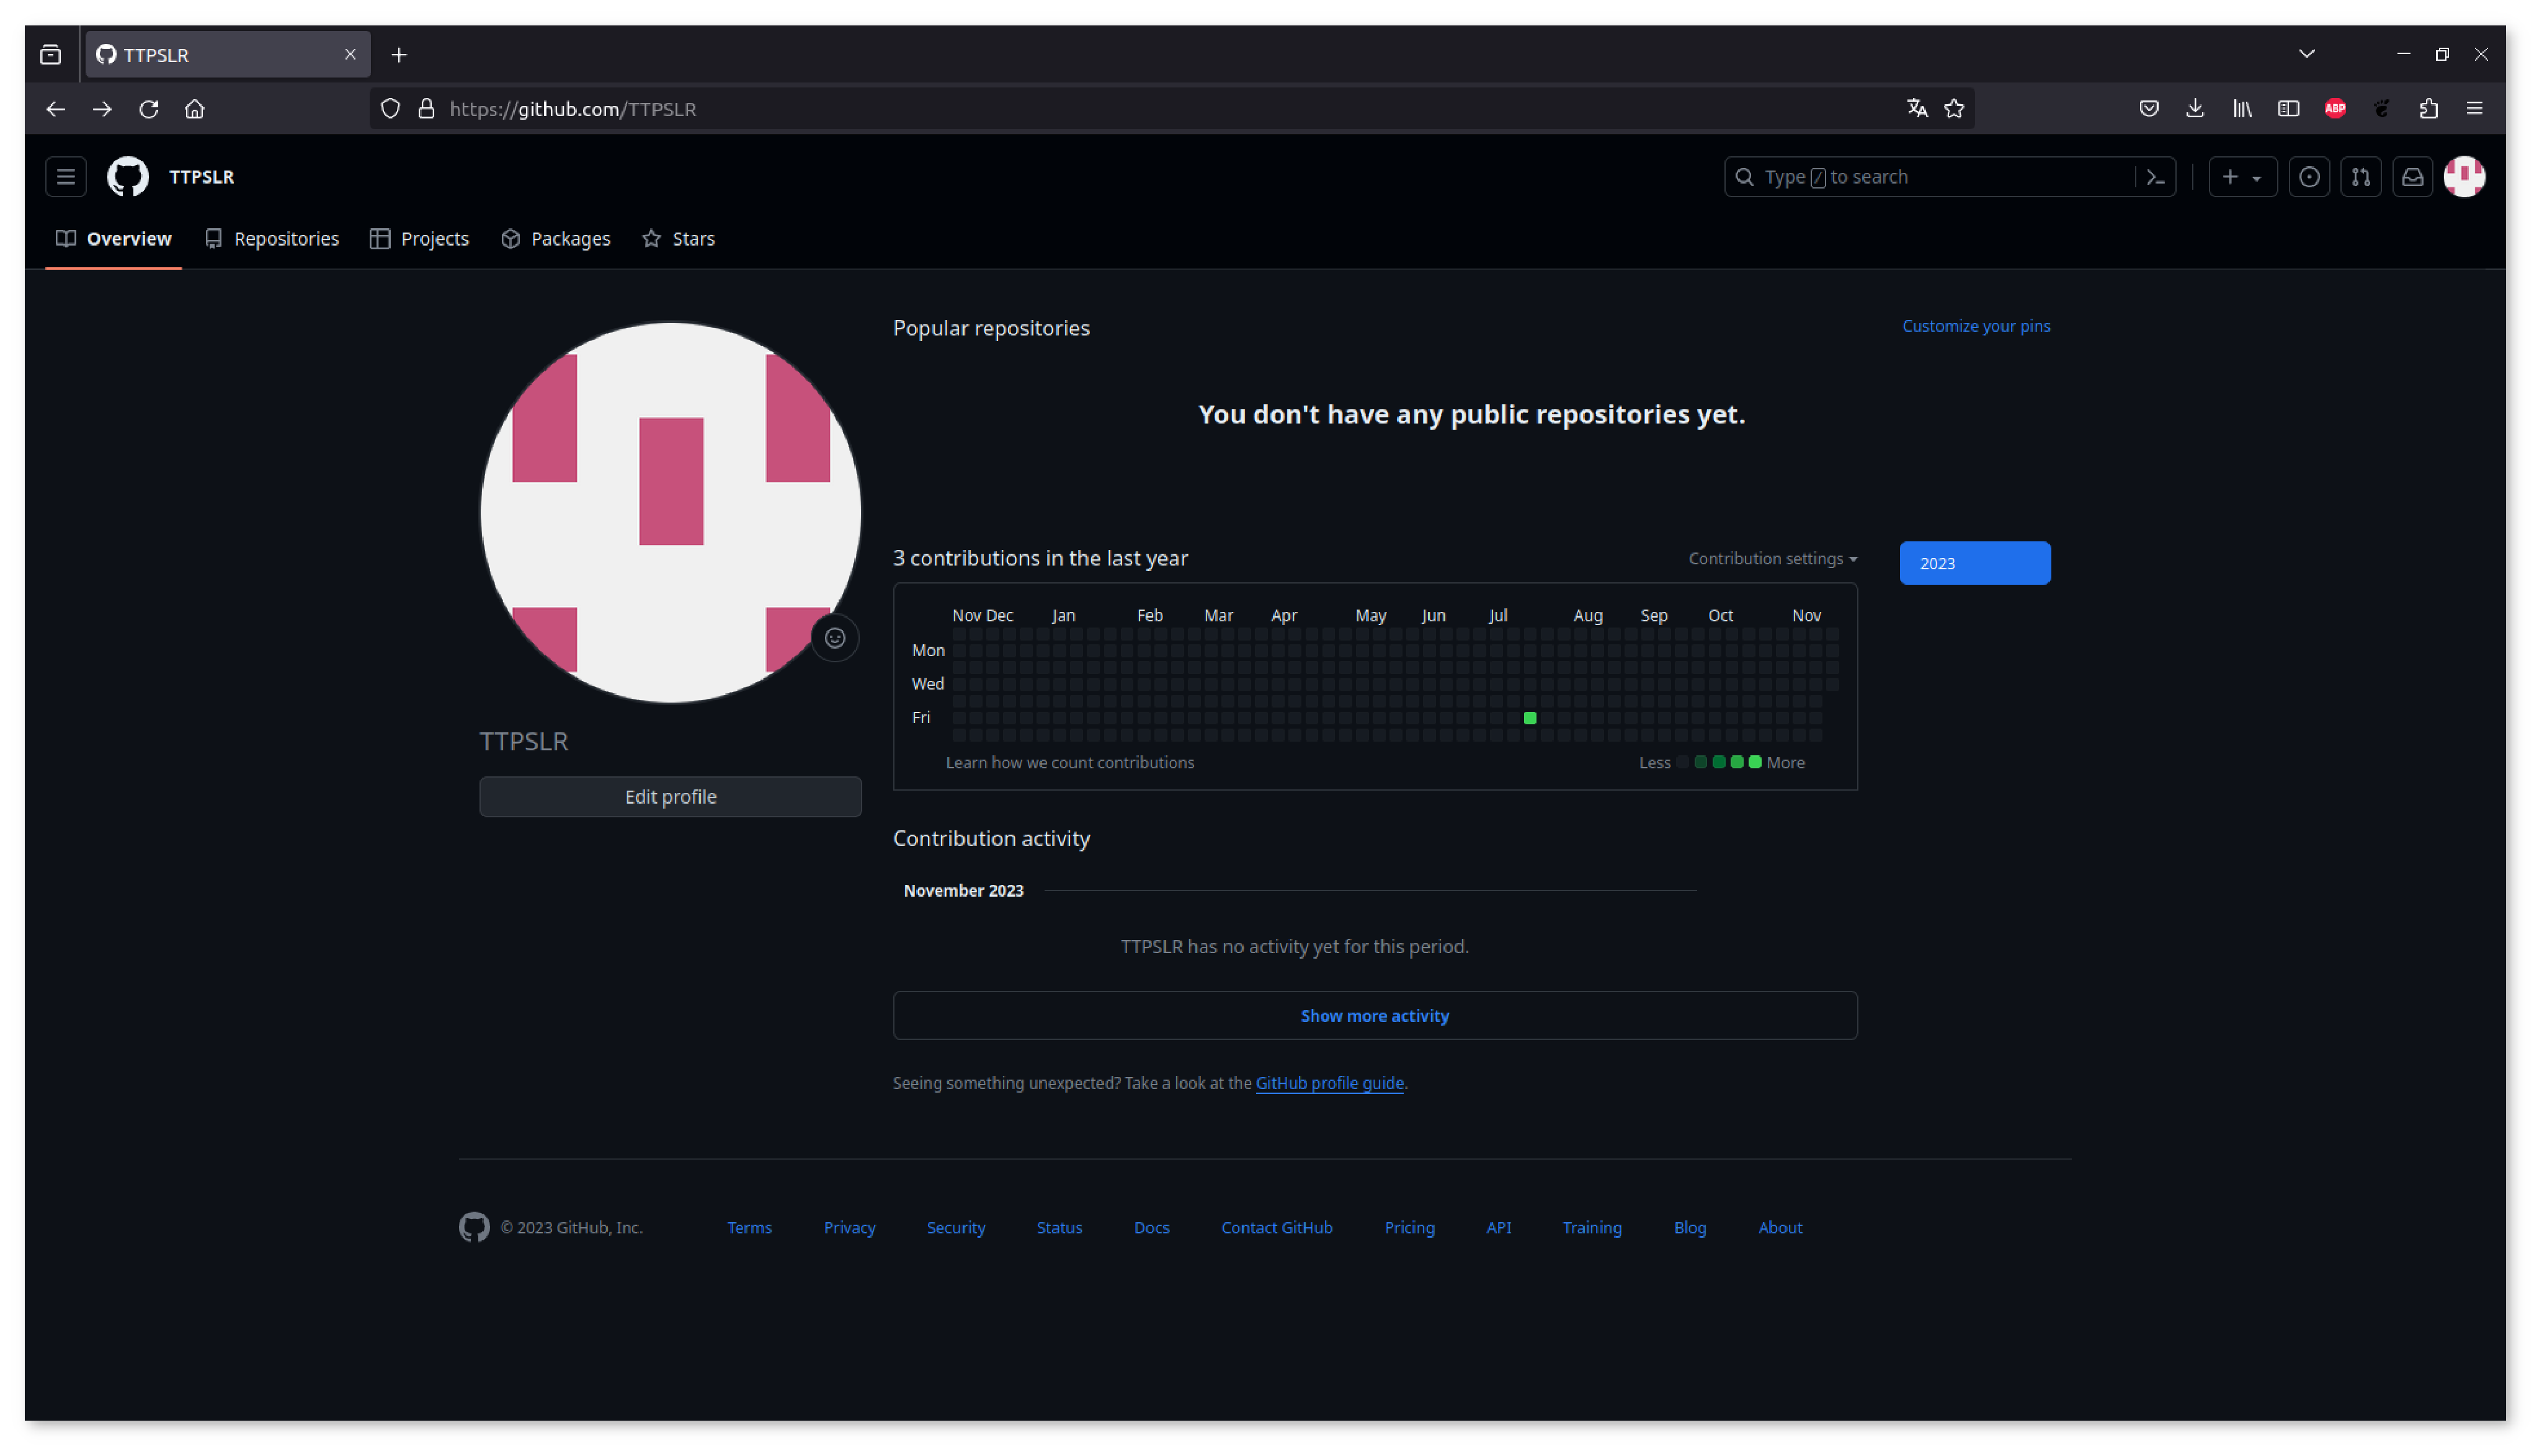
\includegraphics[width=0.85\textwidth,keepaspectratio=true,draft=\ddst]{img/hosts/github/home.eps}
\item \gitlab: \\[0.25cm]
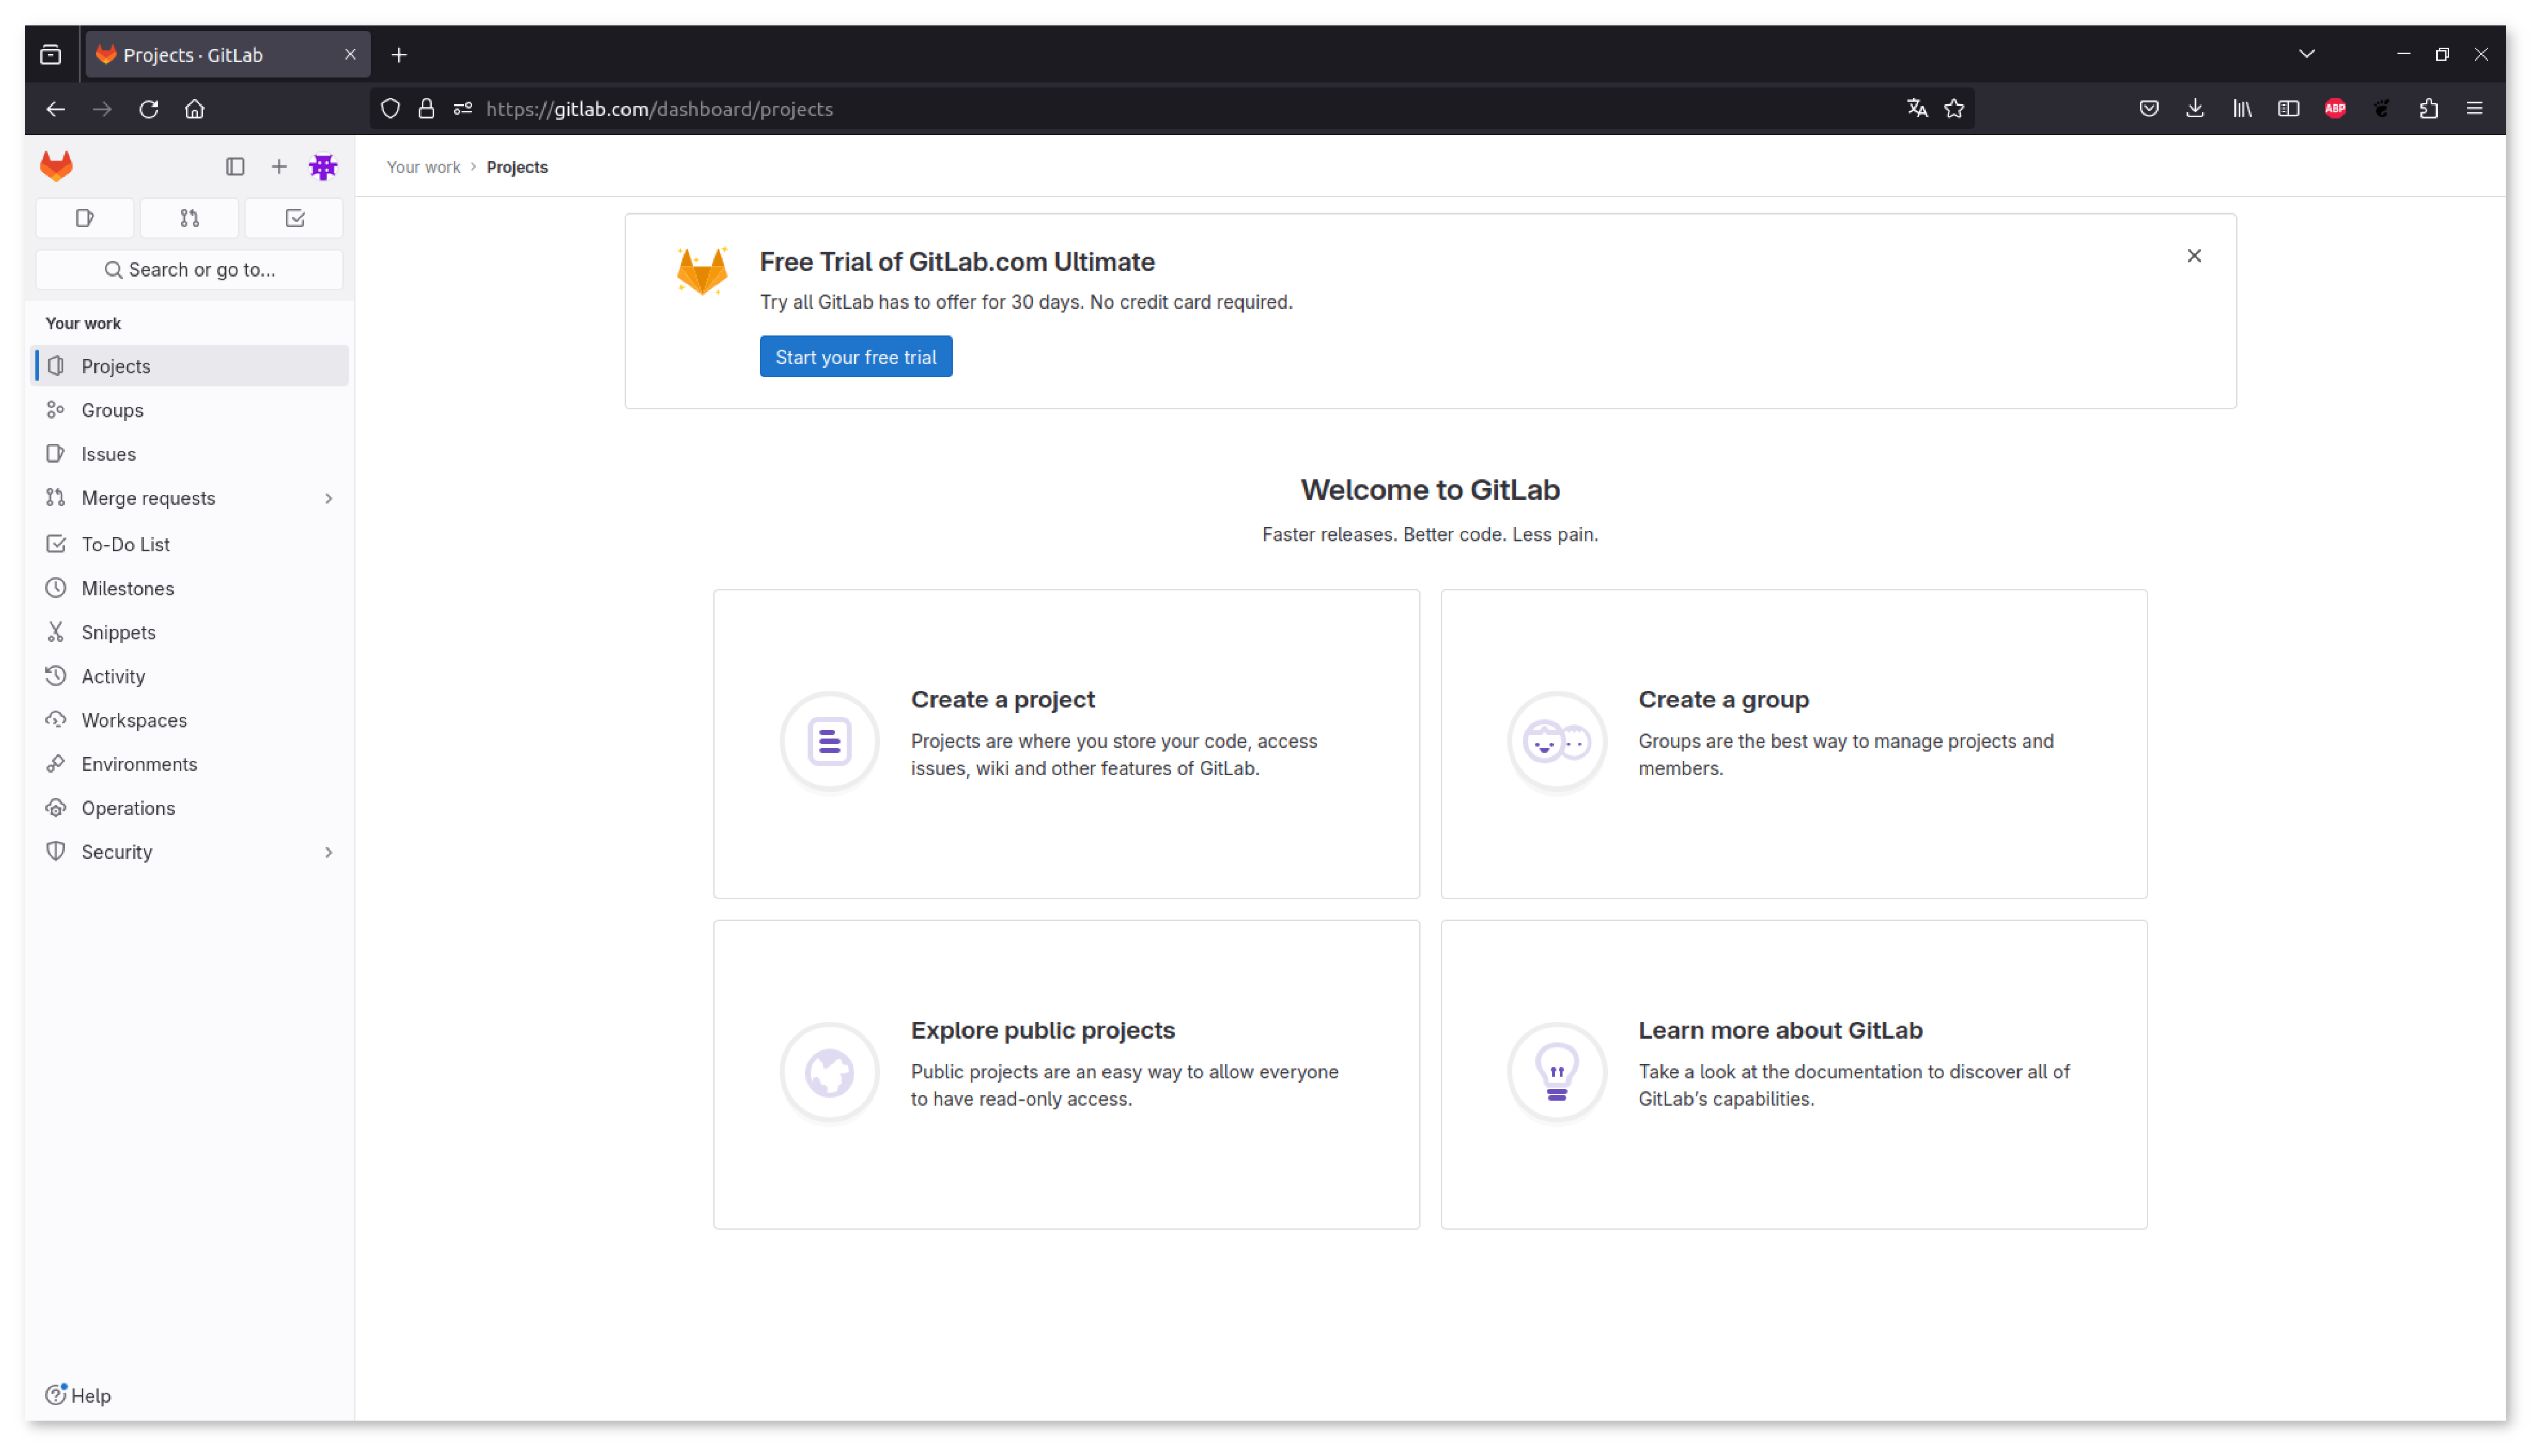
\includegraphics[width=0.85\textwidth,keepaspectratio=true,draft=\ddst]{img/hosts/gitlab/home.eps}
\end{itemize}
In the following examples for both \github\ and \gitlab:
\begin{itemize}
\item the account/group name is: "\texttt{TTPSLR}"
\item the project name is: "\texttt{Program}"
\end{itemize}

\newpage
\section{Creating a repository / project}

The procedure is quite similar, only the denomination changes: 
\begin{itemize}
\item On \github\ the space to store and share your sources is called a "\texttt{repository}"
\item On \gitlab\ the space to store and share your sources is called a "\texttt{project}"
\end{itemize}
\vspace{0.25cm}
\begin{itemize}
\item \github:
\end{itemize}
\vspace{0.5cm}
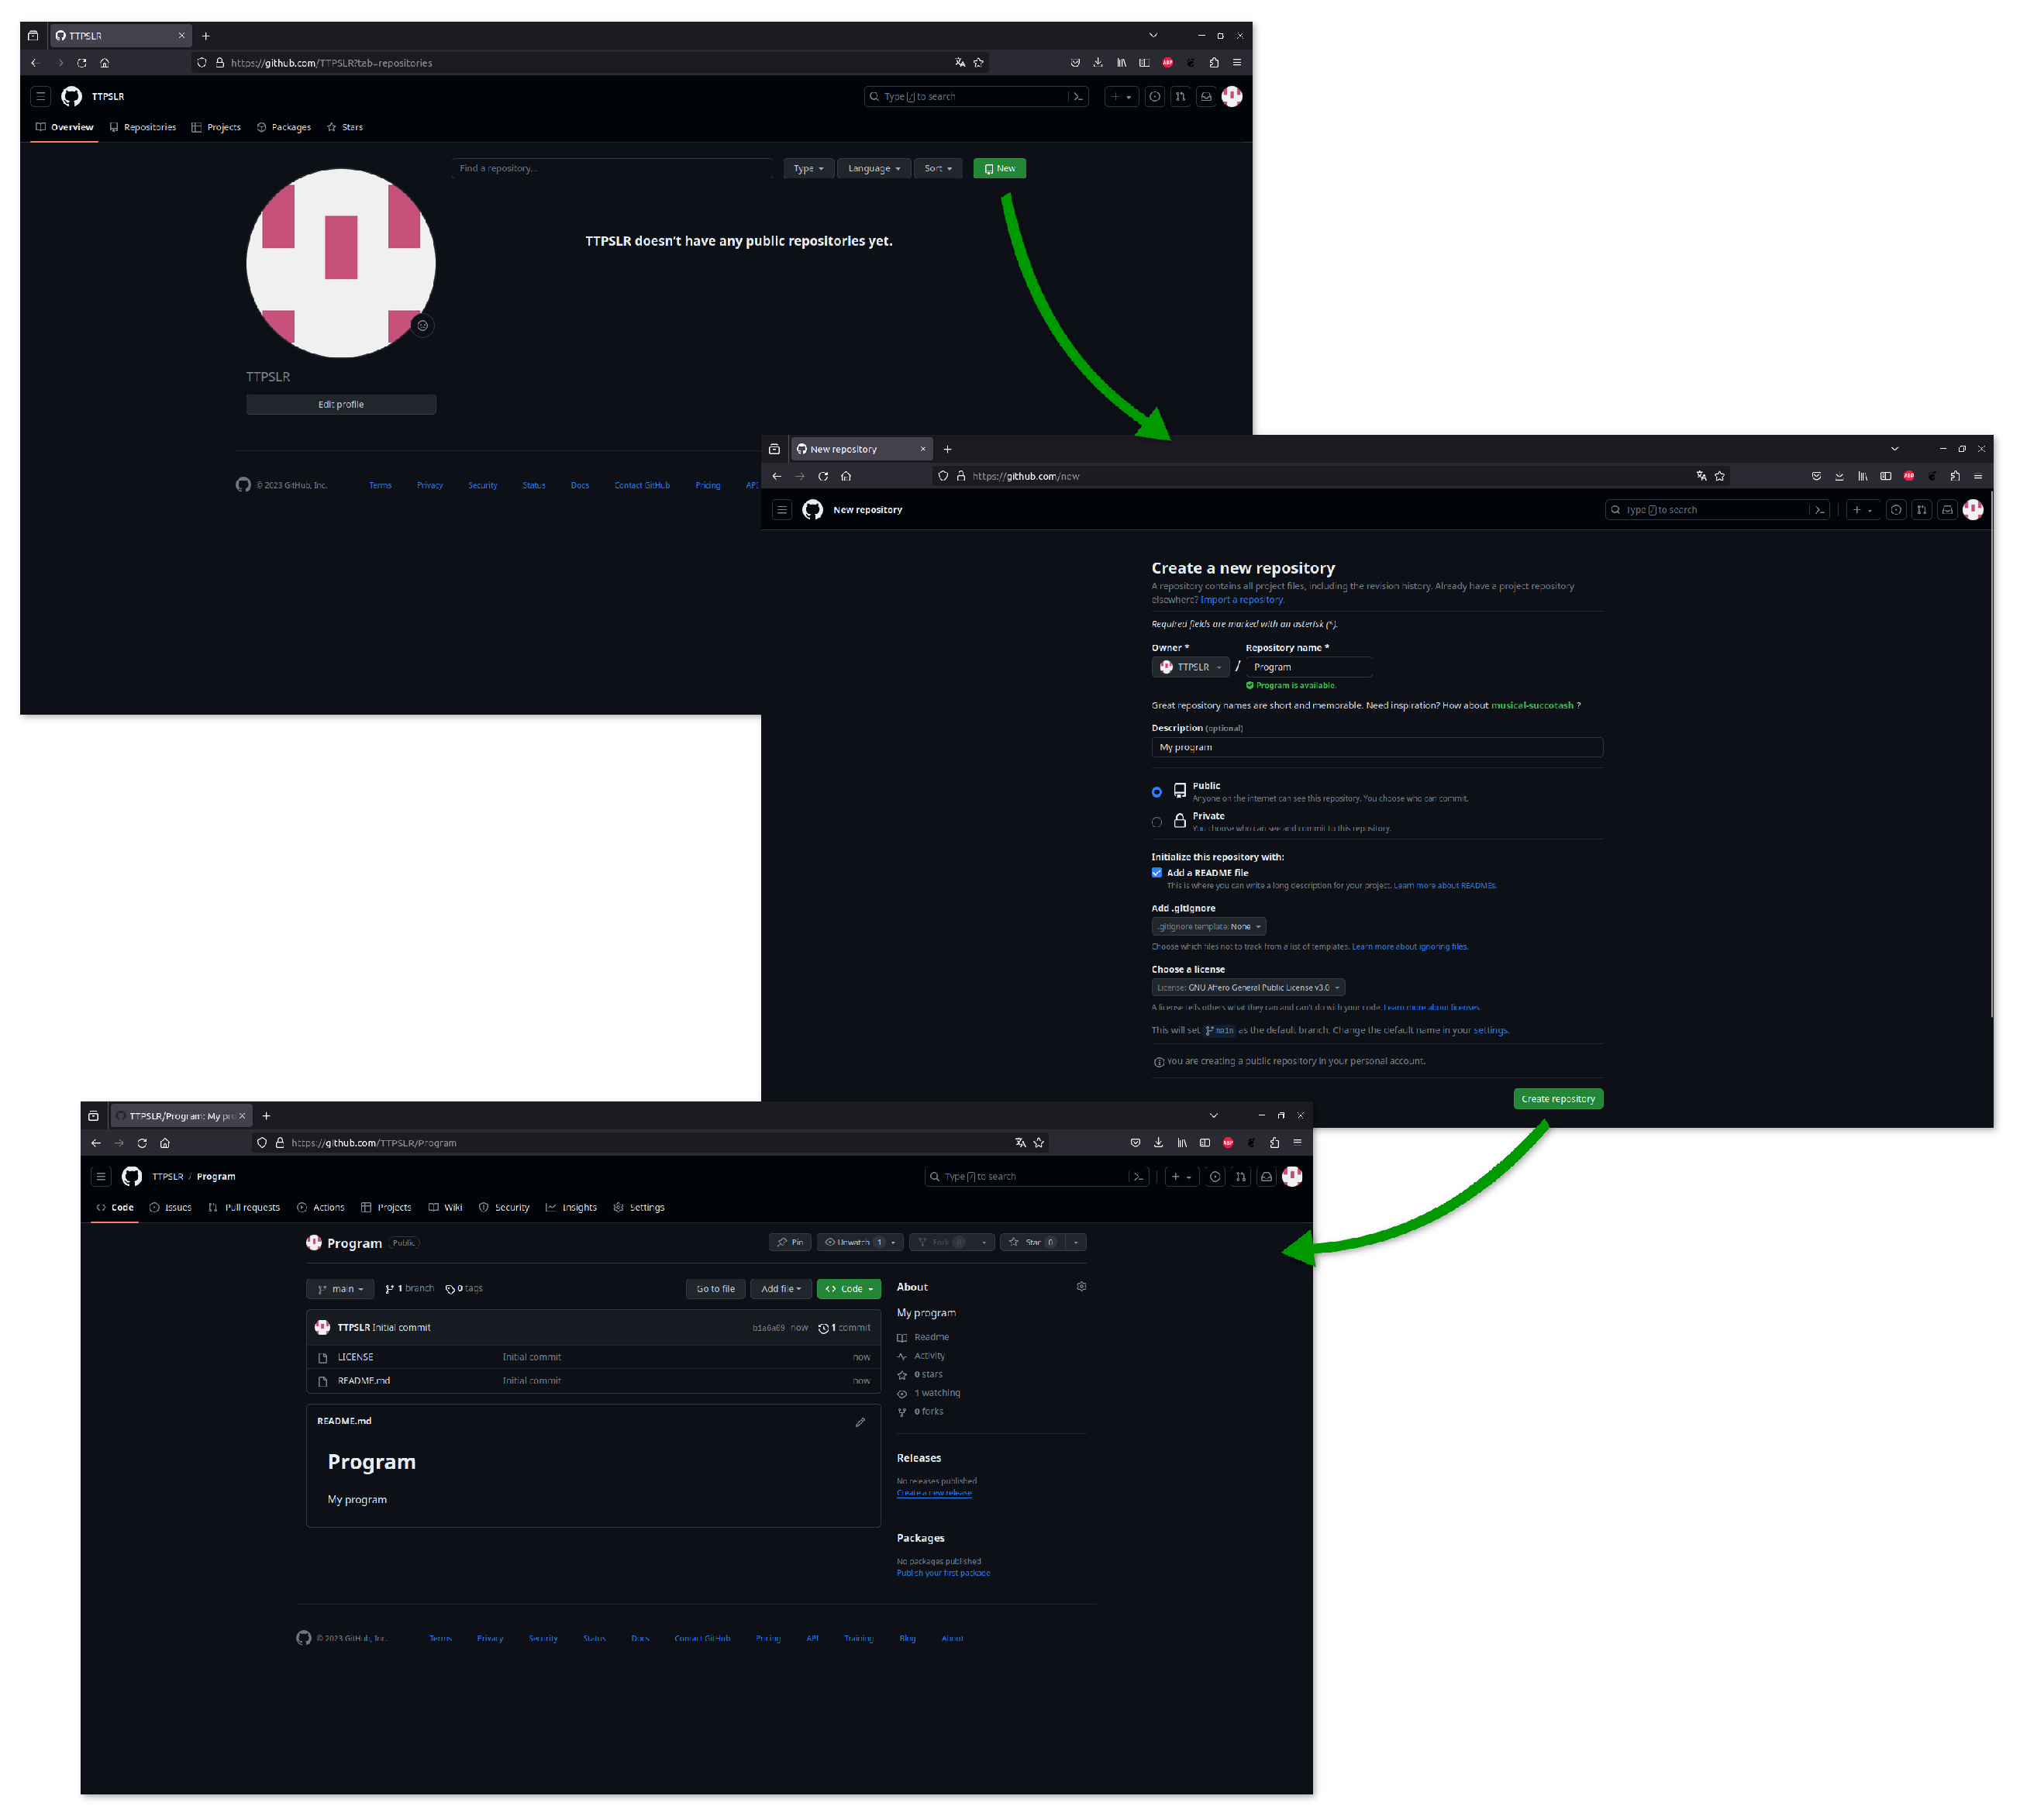
\includegraphics[width=1.0\textwidth,keepaspectratio=true,draft=\ddst]{img/hosts/github/new-p.eps} \\[0.25cm]
\begin{itemize}
\item Open the "\texttt{Repositories}" tab and click on "\texttt{New}"
\item Fill the new project information
\item Click on "\texttt{Create repository}"
\end{itemize}
\newpage
\begin{itemize}
\item \gitlab:
\end{itemize}
\vspace{0.5cm}
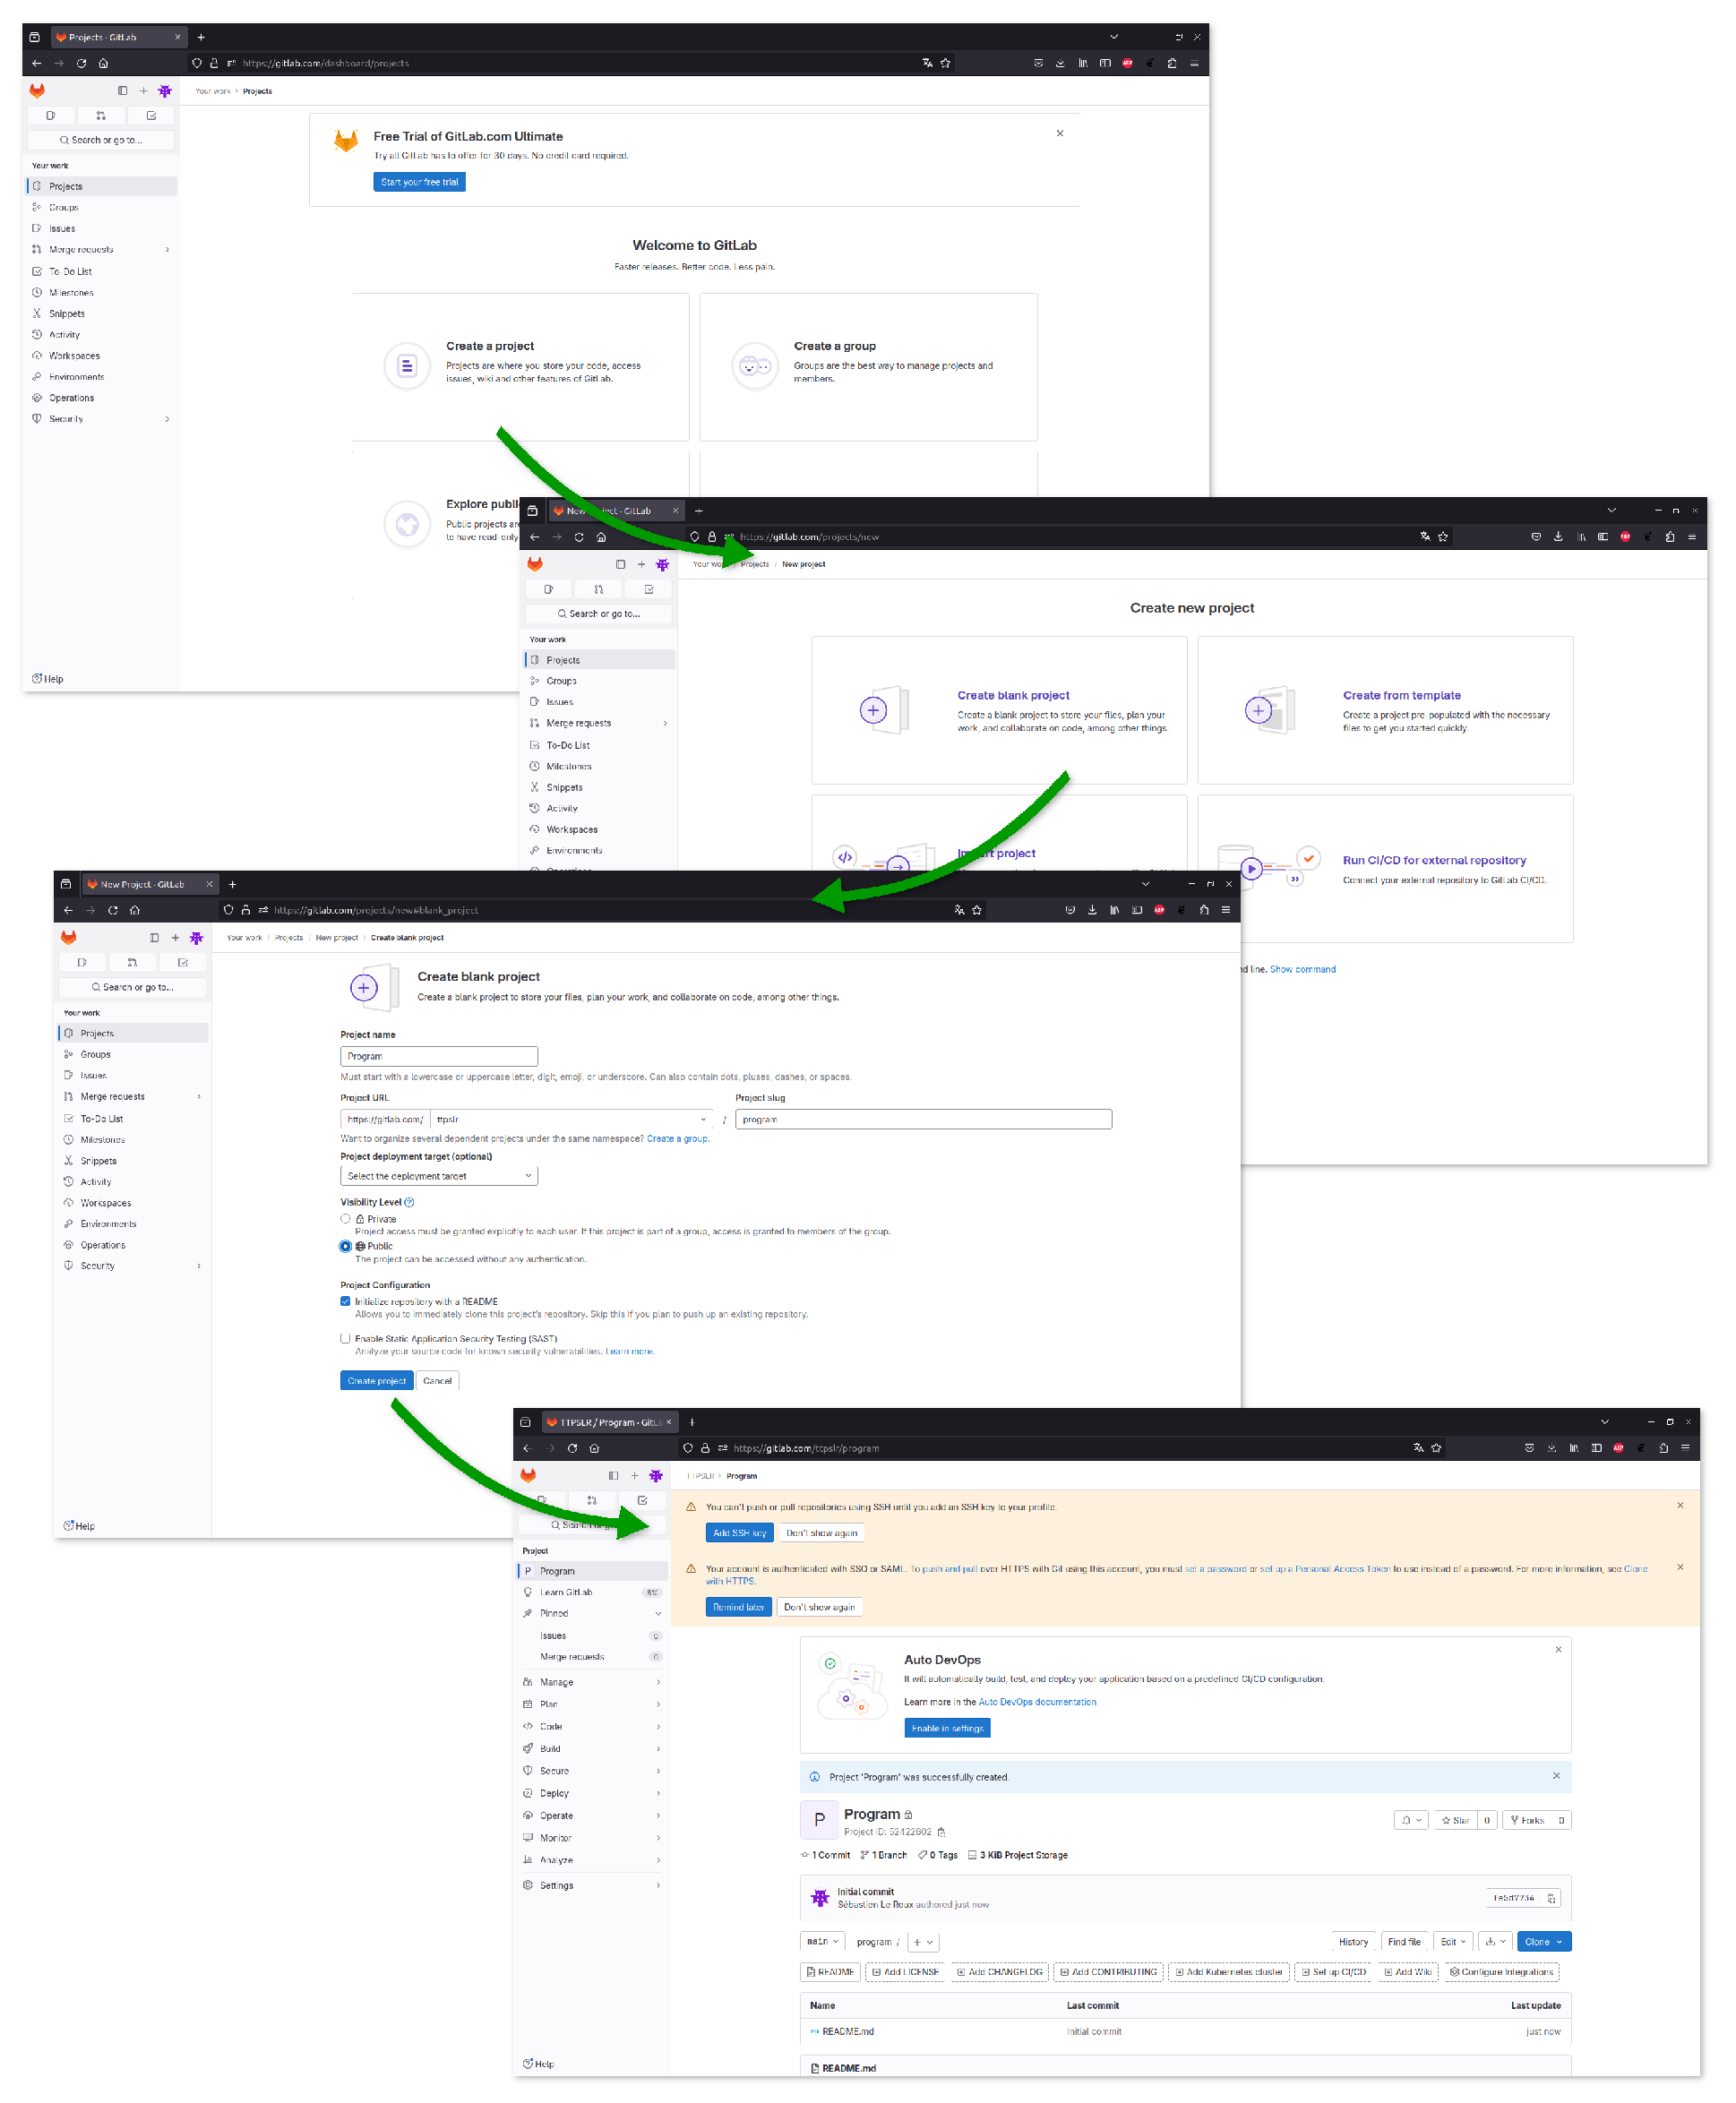
\includegraphics[width=1.0\textwidth,keepaspectratio=true,draft=\ddst]{img/hosts/gitlab/new-p.eps} %\\[0.25cm]
\newpage
\begin{itemize}
\item Click on "\texttt{Create project}"
\item Click on "\texttt{Create blank project}"
\item Fill the new project information
\item Click on "\texttt{Create project}"
\end{itemize}

\section{SSH encryption keys}

Immediately after creating your first project, setup the SSH encryption keys. 
These keys are digital tokens that prove your identity when performing actions to update the on line repository using Git. 

\subsection{Generating SSH encryption keys}

If not done already you need first to create SSH encryption keys, this is done using a command line utility: 
\begin{script}
\fprompt{~} \bftt{ssh-keygen} \rtt{-t} \dgtt{ed25519}
\end{script}
"\bftt{ssh-keygen}" generates the key, the "\rtt{-t}" option is used to define the type of encoding, in the example "\dgtt{ed25519}" that stands for \href{https://en.wikipedia.org/wiki/EdDSA}{Edwards-curve Digital Signature Algorithm} which is the most secured standardization these days.  \\
2 files, to be stored in "\texttt{\textasciitilde/.ssh}", will be created by the previous command:
\begin{itemize}
\item A private key, that decipher (act like a key), and that must remains on your computer: 
\begin{scripti}
~/.ssh/id\_ed25519
\end{scripti} \\
\vspace{-1.5cm}
\item A matching public key, that encrypts (acts like a door), used on remote system(s):
\begin{scripti}
~/.ssh/id\_ed25519.pub
\end{scripti} \\[-0.65cm]
\noindent Which content looks like: 
{\scriptsize{
\begin{scripti}
\fprompt{~} cat ~/.ssh/id\_ed25519.pub
ssh-ed25519 AAAAC3NzaC1lZDI1NTE5AAAAIG1TIYyaRZIlFU40NH8QAxXK8SSgl07Thop6CGzcVg0j user@host
\end{scripti}}} \\
\vspace{-1.5cm}
\end{itemize}
For more about asymmetric keys algorithms: \href{https://en.wikipedia.org/wiki/Public-key\_cryptography}{https://en.wikipedia.org/wiki/Public-key\_cryptography}
\newpage

\subsection{Adding the keys to GitHub / GitLab}

Now you need to add the public key to your \github\ / \gitlab\ repository: 
\begin{itemize}
\item \github\ (see figure~\ref{kgithub}):
\begin{itemize}
\item Click on the profile logo and click on "\texttt{Settings}"
\item Click on the "\texttt{SSH and GPG keys}"
\item Click on "\texttt{Create repository}"
\item Click on "\texttt{New SSH key}"
\item Adjust the key information:
\begin{itemize}
\item Give the key a title name
\item Select the key type: "\texttt{Authentication key}" 
\item Copy / paste the content of public key file in the text box
\end{itemize}
\item Finally click on "\texttt{Add SSH key}"
\end{itemize}
\item \gitlab\ (see figure~\ref{kgitlab}):
\begin{itemize}
\item Click on shortcut button "\texttt{Add SSH key}" \\
Alternatively click on your public avatar (squared in red in figure~\ref{kgitlab}), \\
click on "\texttt{Preferences}", then click on "\texttt{SSH Keys}"
\item Click on the "\texttt{Add new key}"
\item Adjust the key information:
\begin{itemize}
\item Copy / paste the content of public key file in the text box
\item Give the key a title name
\item Select the key type: "\texttt{Authentication}" or "\texttt{Authentication \& Signing}" 
\end{itemize}
\item Finally click on "\texttt{Add key}"
\item Optionally go back the "\texttt{User Settings} $\Longrightarrow$ \texttt{SSH Keys}" tab to visualize that the key is properly stored
\end{itemize}
\end{itemize}
As soon as the keys have been installed you are ready to work with your on line repository. 

\begin{figure}[!p]
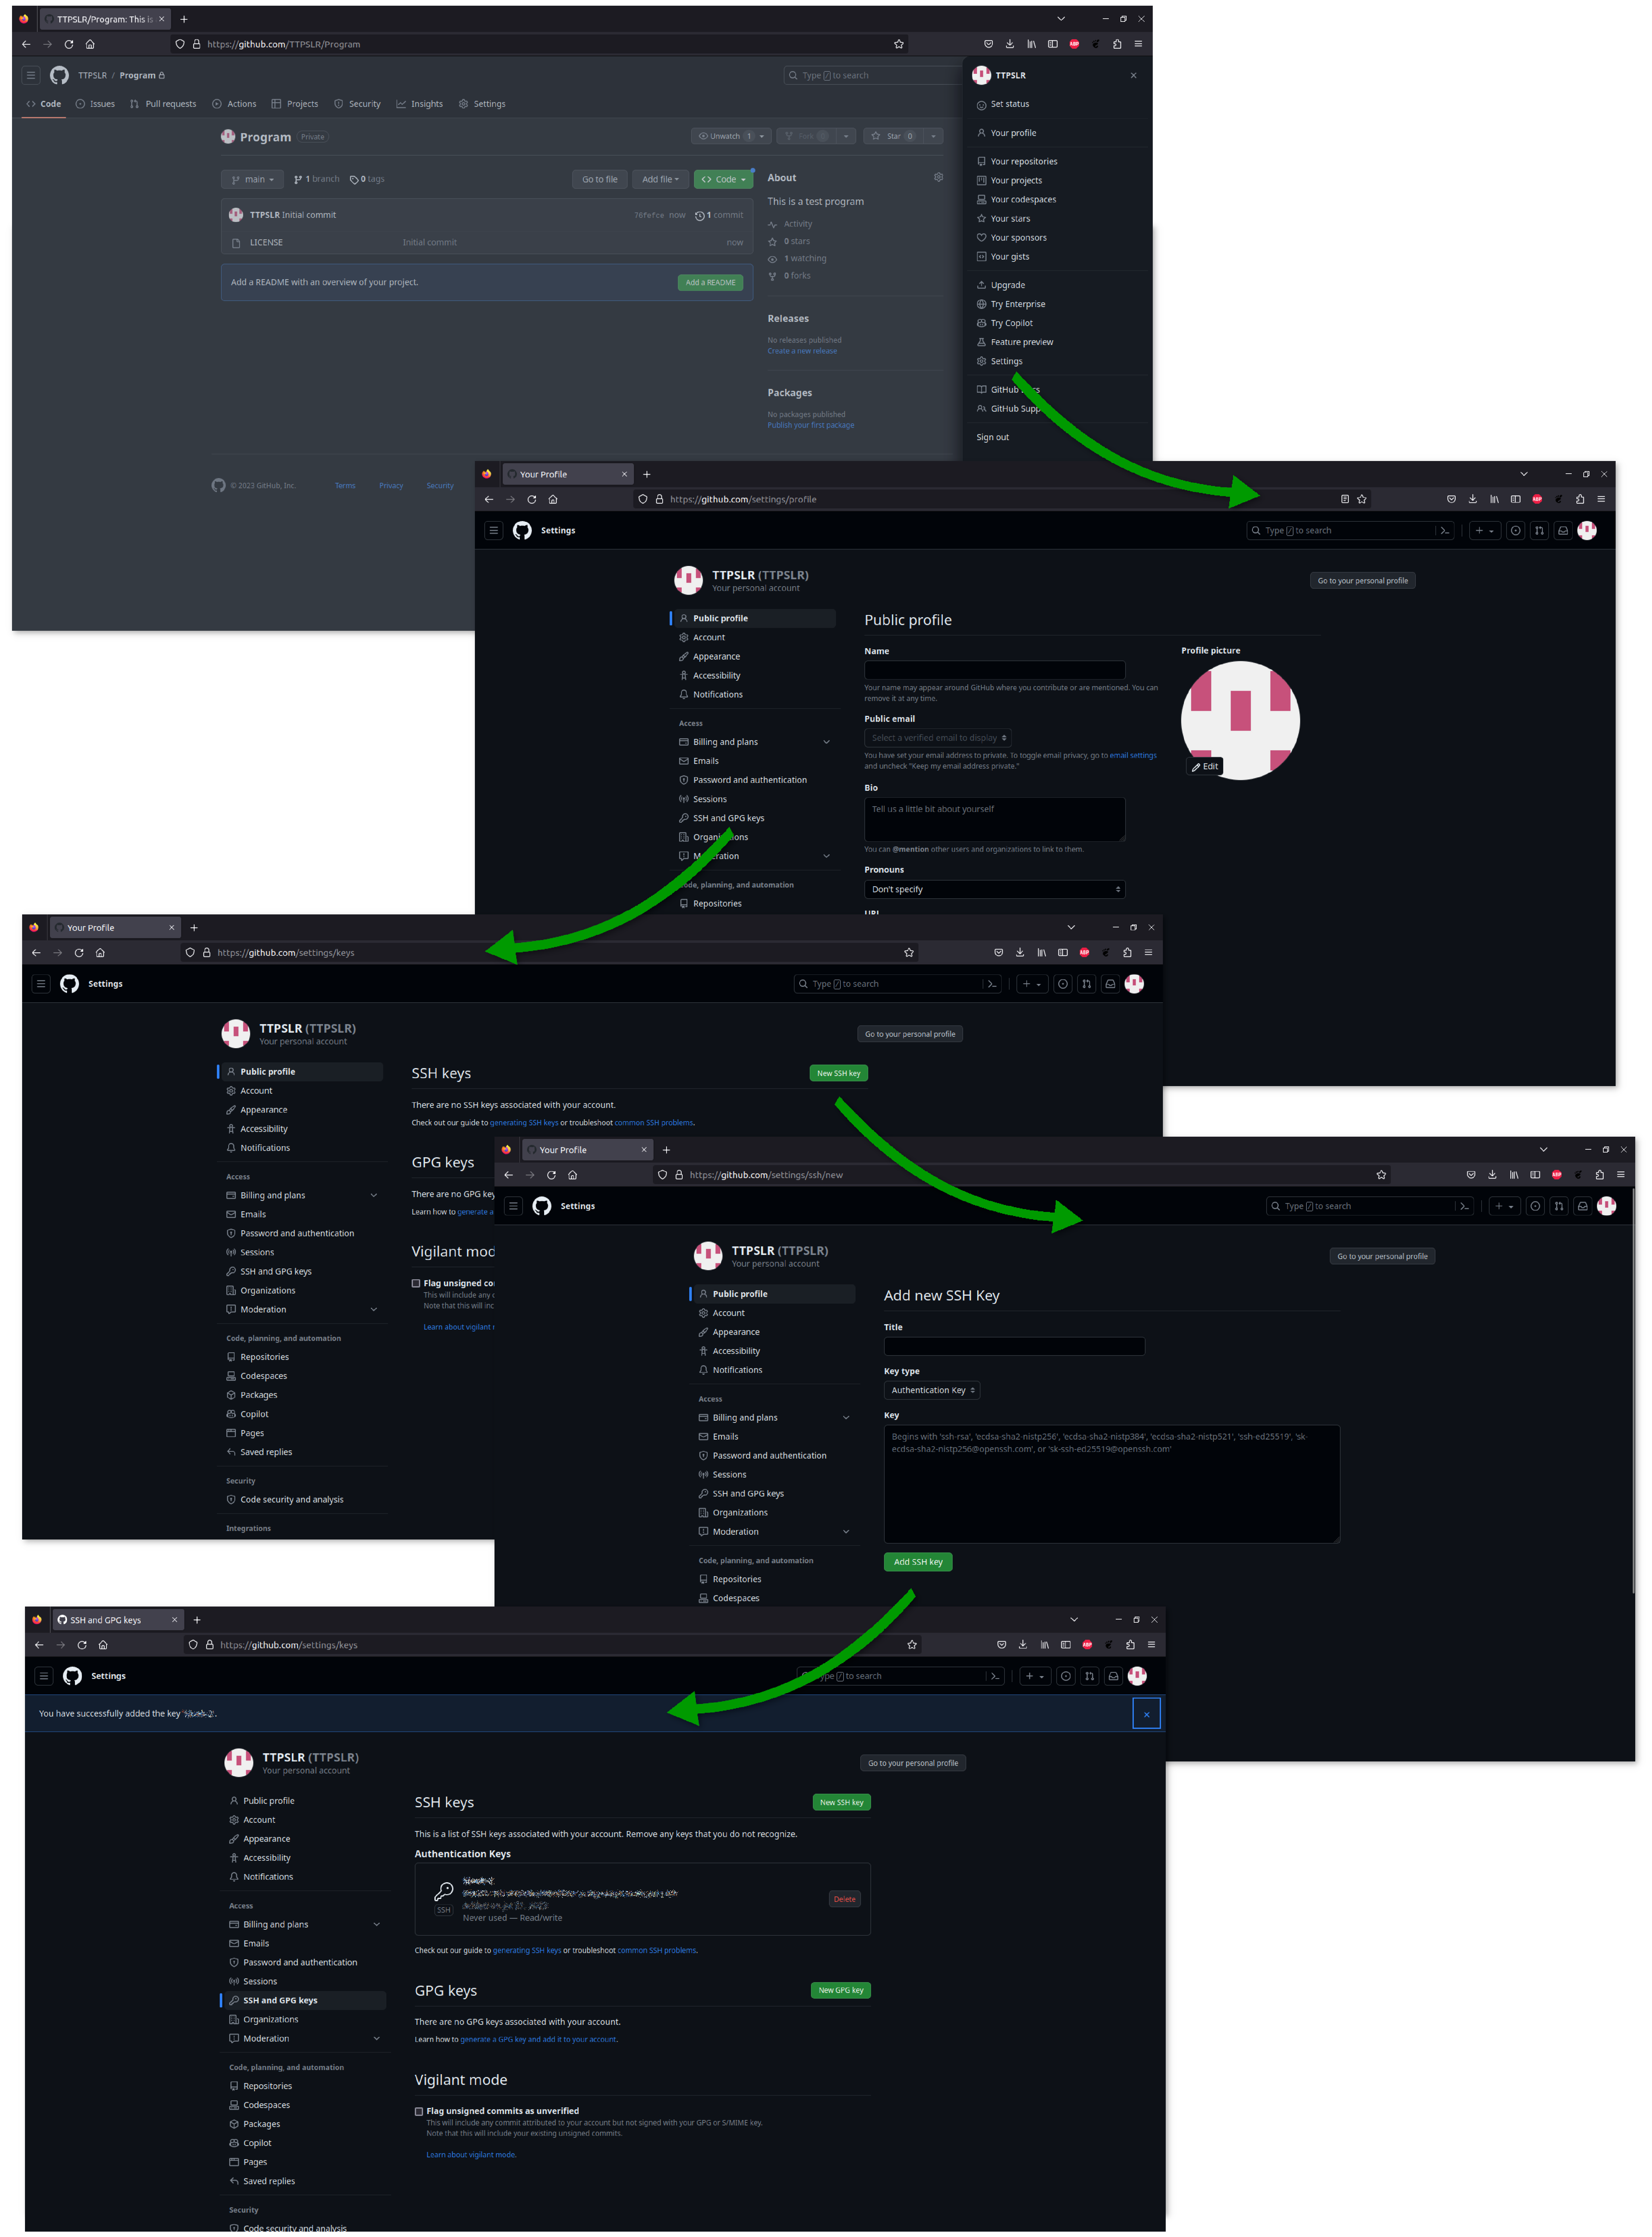
\includegraphics[width=1.0\textwidth,keepaspectratio=true,draft=\ddst]{img/hosts/github/keys.eps} 
\caption{Adding a SSH key on \github\label{kgithub}}
\end{figure}

\begin{figure}[!p]

\includegraphics[width=1.0\textwidth,keepaspectratio=true,draft=\ddst]{img/hosts/gitlab/keys.eps} 
\caption{Adding a SSH key on \gitlab\label{kgitlab}}
\end{figure}

\clearpage

\section{Branch protection}

If you are managing collaborative project, with several developers being able to push commits to the Git (and \github\ or \gitlab) repository branch(es), 
then you need to ensure that branch(es) of your project is (are) being protected against errors, ensuring that changes are handled by the project manager, or designated and selected developers. \\
To do that you need to enable, and adjust, branch(es) protection:
\begin{itemize}
\item \github\ (see figure~\ref{bgithub}):
\begin{itemize}
\item Click on "\texttt{Settings}"
\item Click on "\texttt{Branches}"
\item Click on "\texttt{Add branch protection rule}"
\item Choose branch name and adjust the protection level for this target branch of your project
\item Scroll down and click on "\texttt{Create}"
\end{itemize}
Note that on \github\ no branch protection is in place at the beginning to this step is really important. 
\item \gitlab:
\begin{itemize}
\item Default main branch protection for all your projects (see figure~\ref{mbgitlab}):
\begin{itemize}
\item Click on "\texttt{Settings}" $\Longrightarrow$ "\texttt{Repository}"
\item In front of "\texttt{Default branch}" click on "\texttt{Expand}"
\item Ensure that "\texttt{Fully protected}" 
\end{itemize}
\item Other branches protection (see figure~\ref{bpgitlab}):
\begin{itemize}
\item Click on "\texttt{Settings}" $\Longrightarrow$ "\texttt{Repository}"
\item In front of "\texttt{Protected branches}" click on "\texttt{Expand}"
\item Adjust the protection level for the target branch of your project
\end{itemize}
\end{itemize}
On \gitlab\ however branch protection should already be in place for the main branch.
\end{itemize}

\begin{figure}[!p]
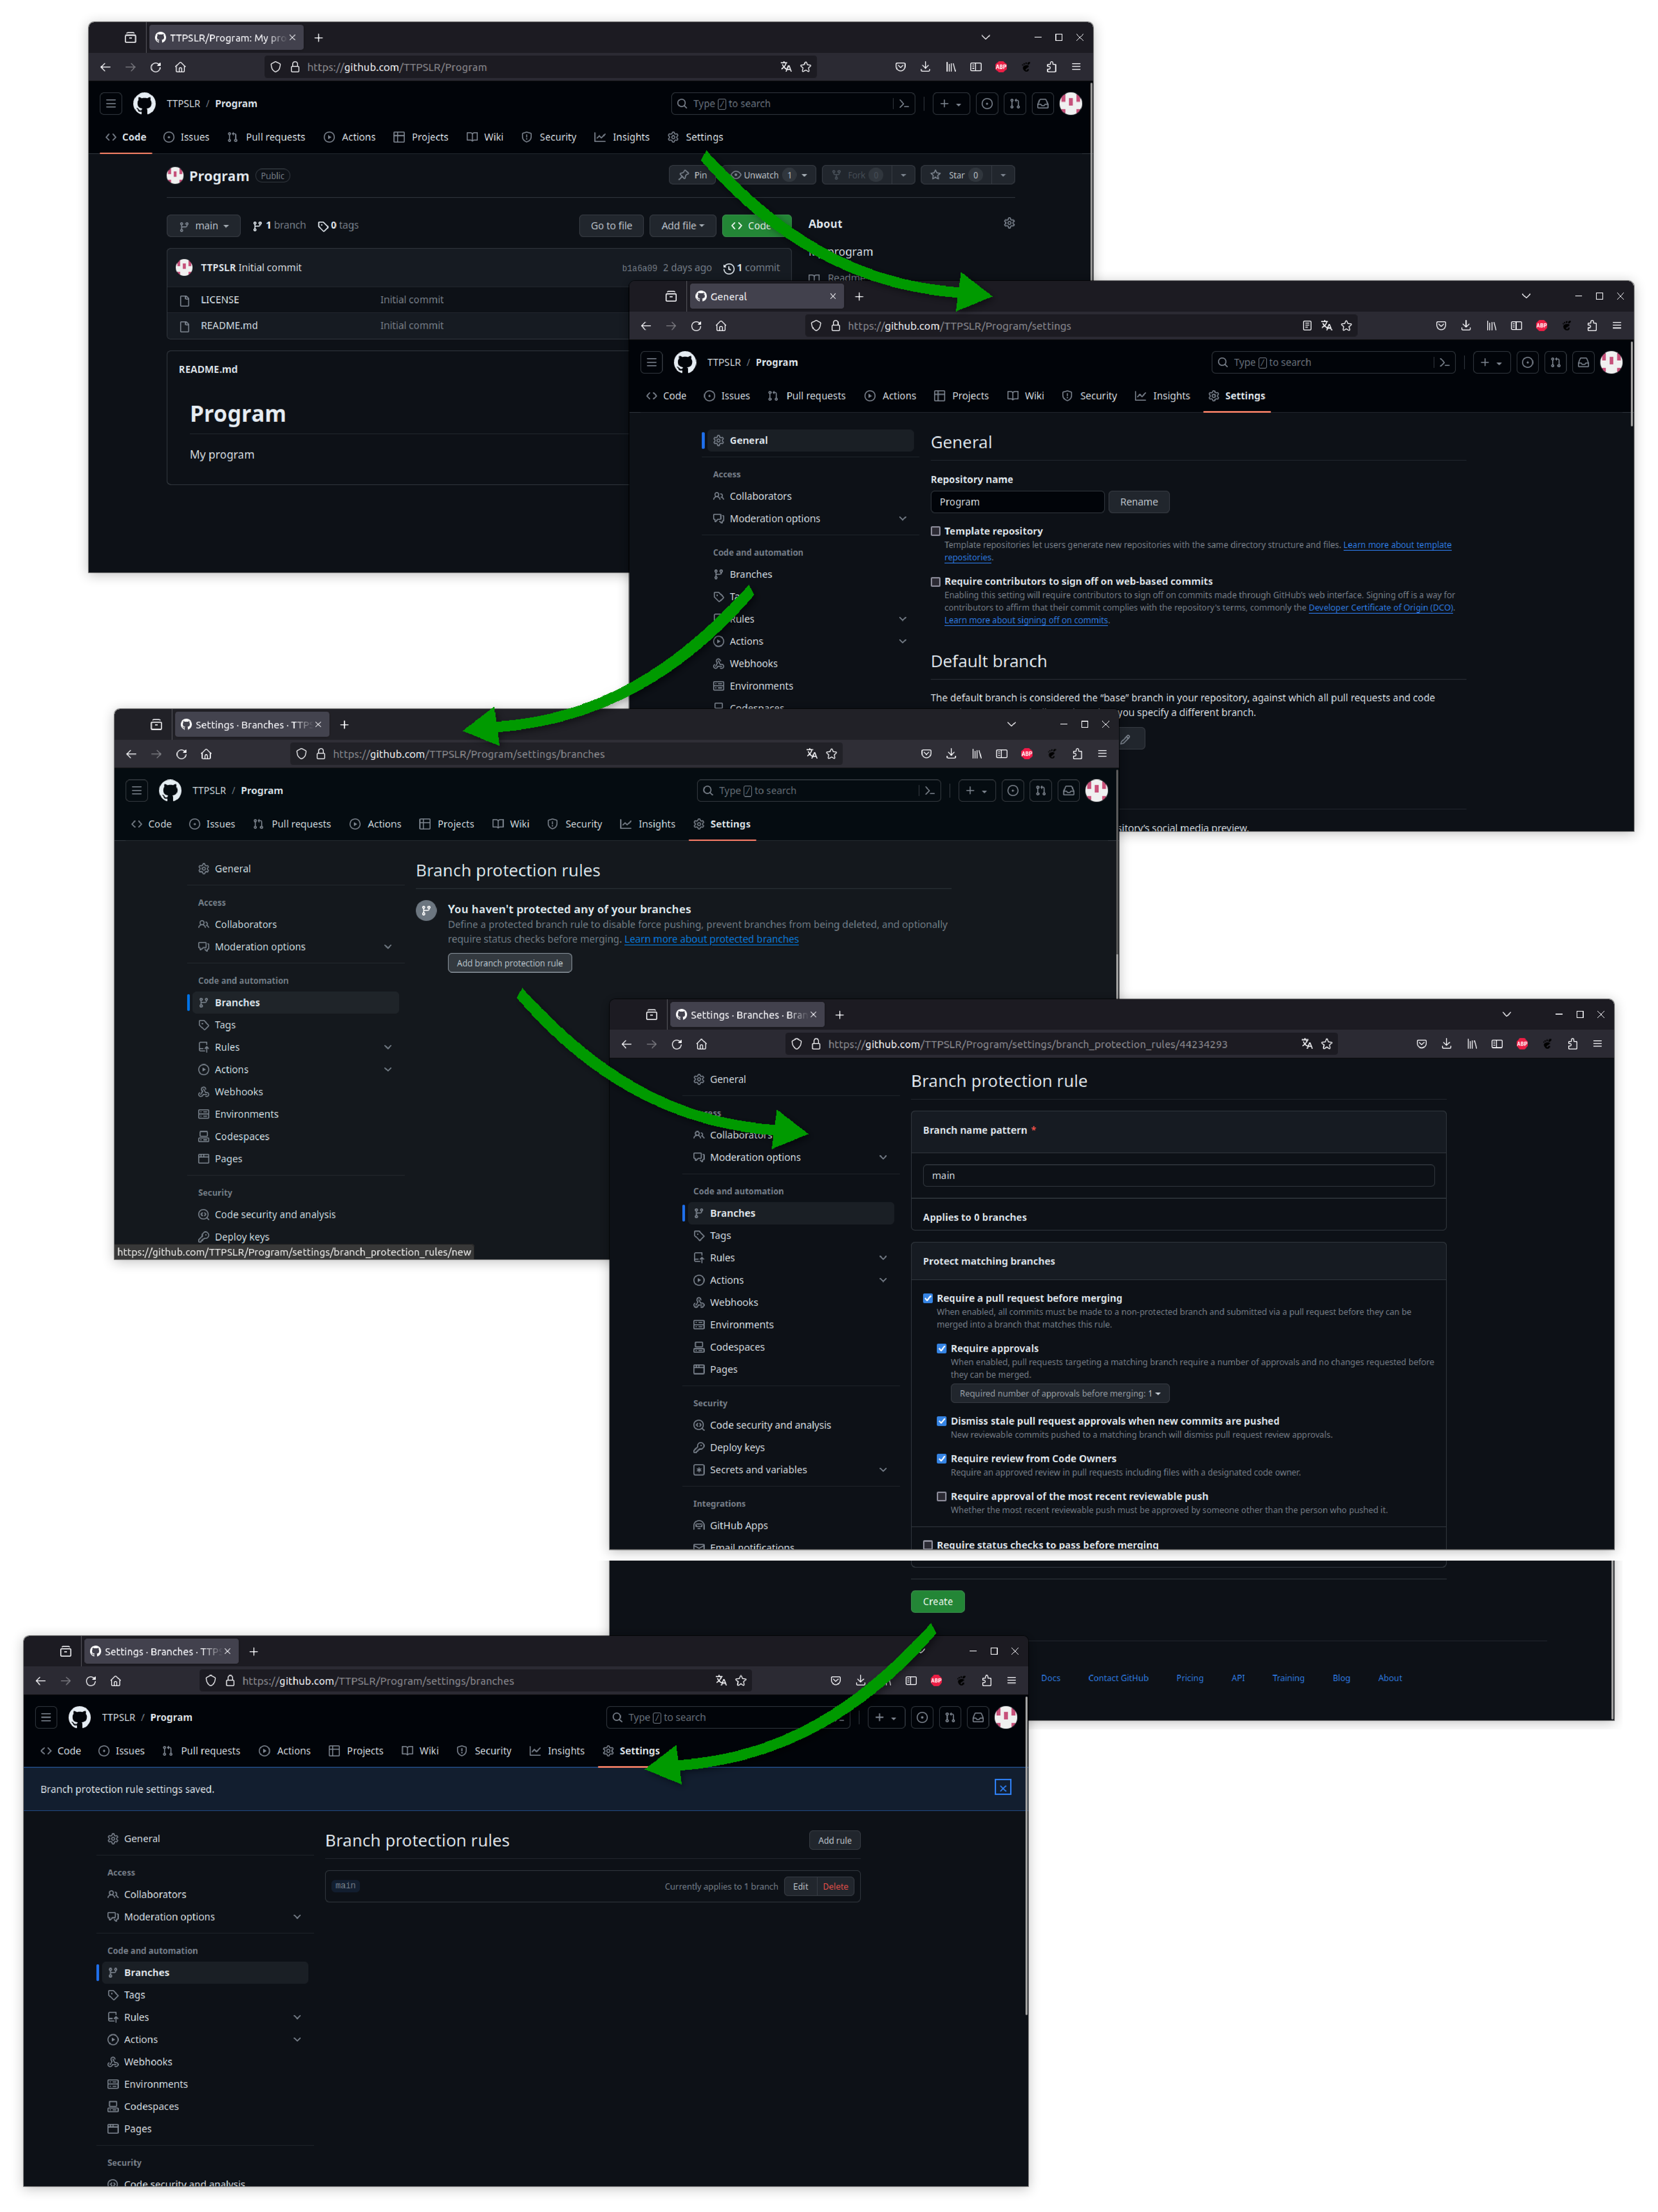
\includegraphics[width=1.0\textwidth,keepaspectratio=true,draft=\ddst]{img/hosts/github/branch.eps} 
\caption{Project branch projection on \github\label{bgithub}}
\end{figure}

\begin{figure}[!p]
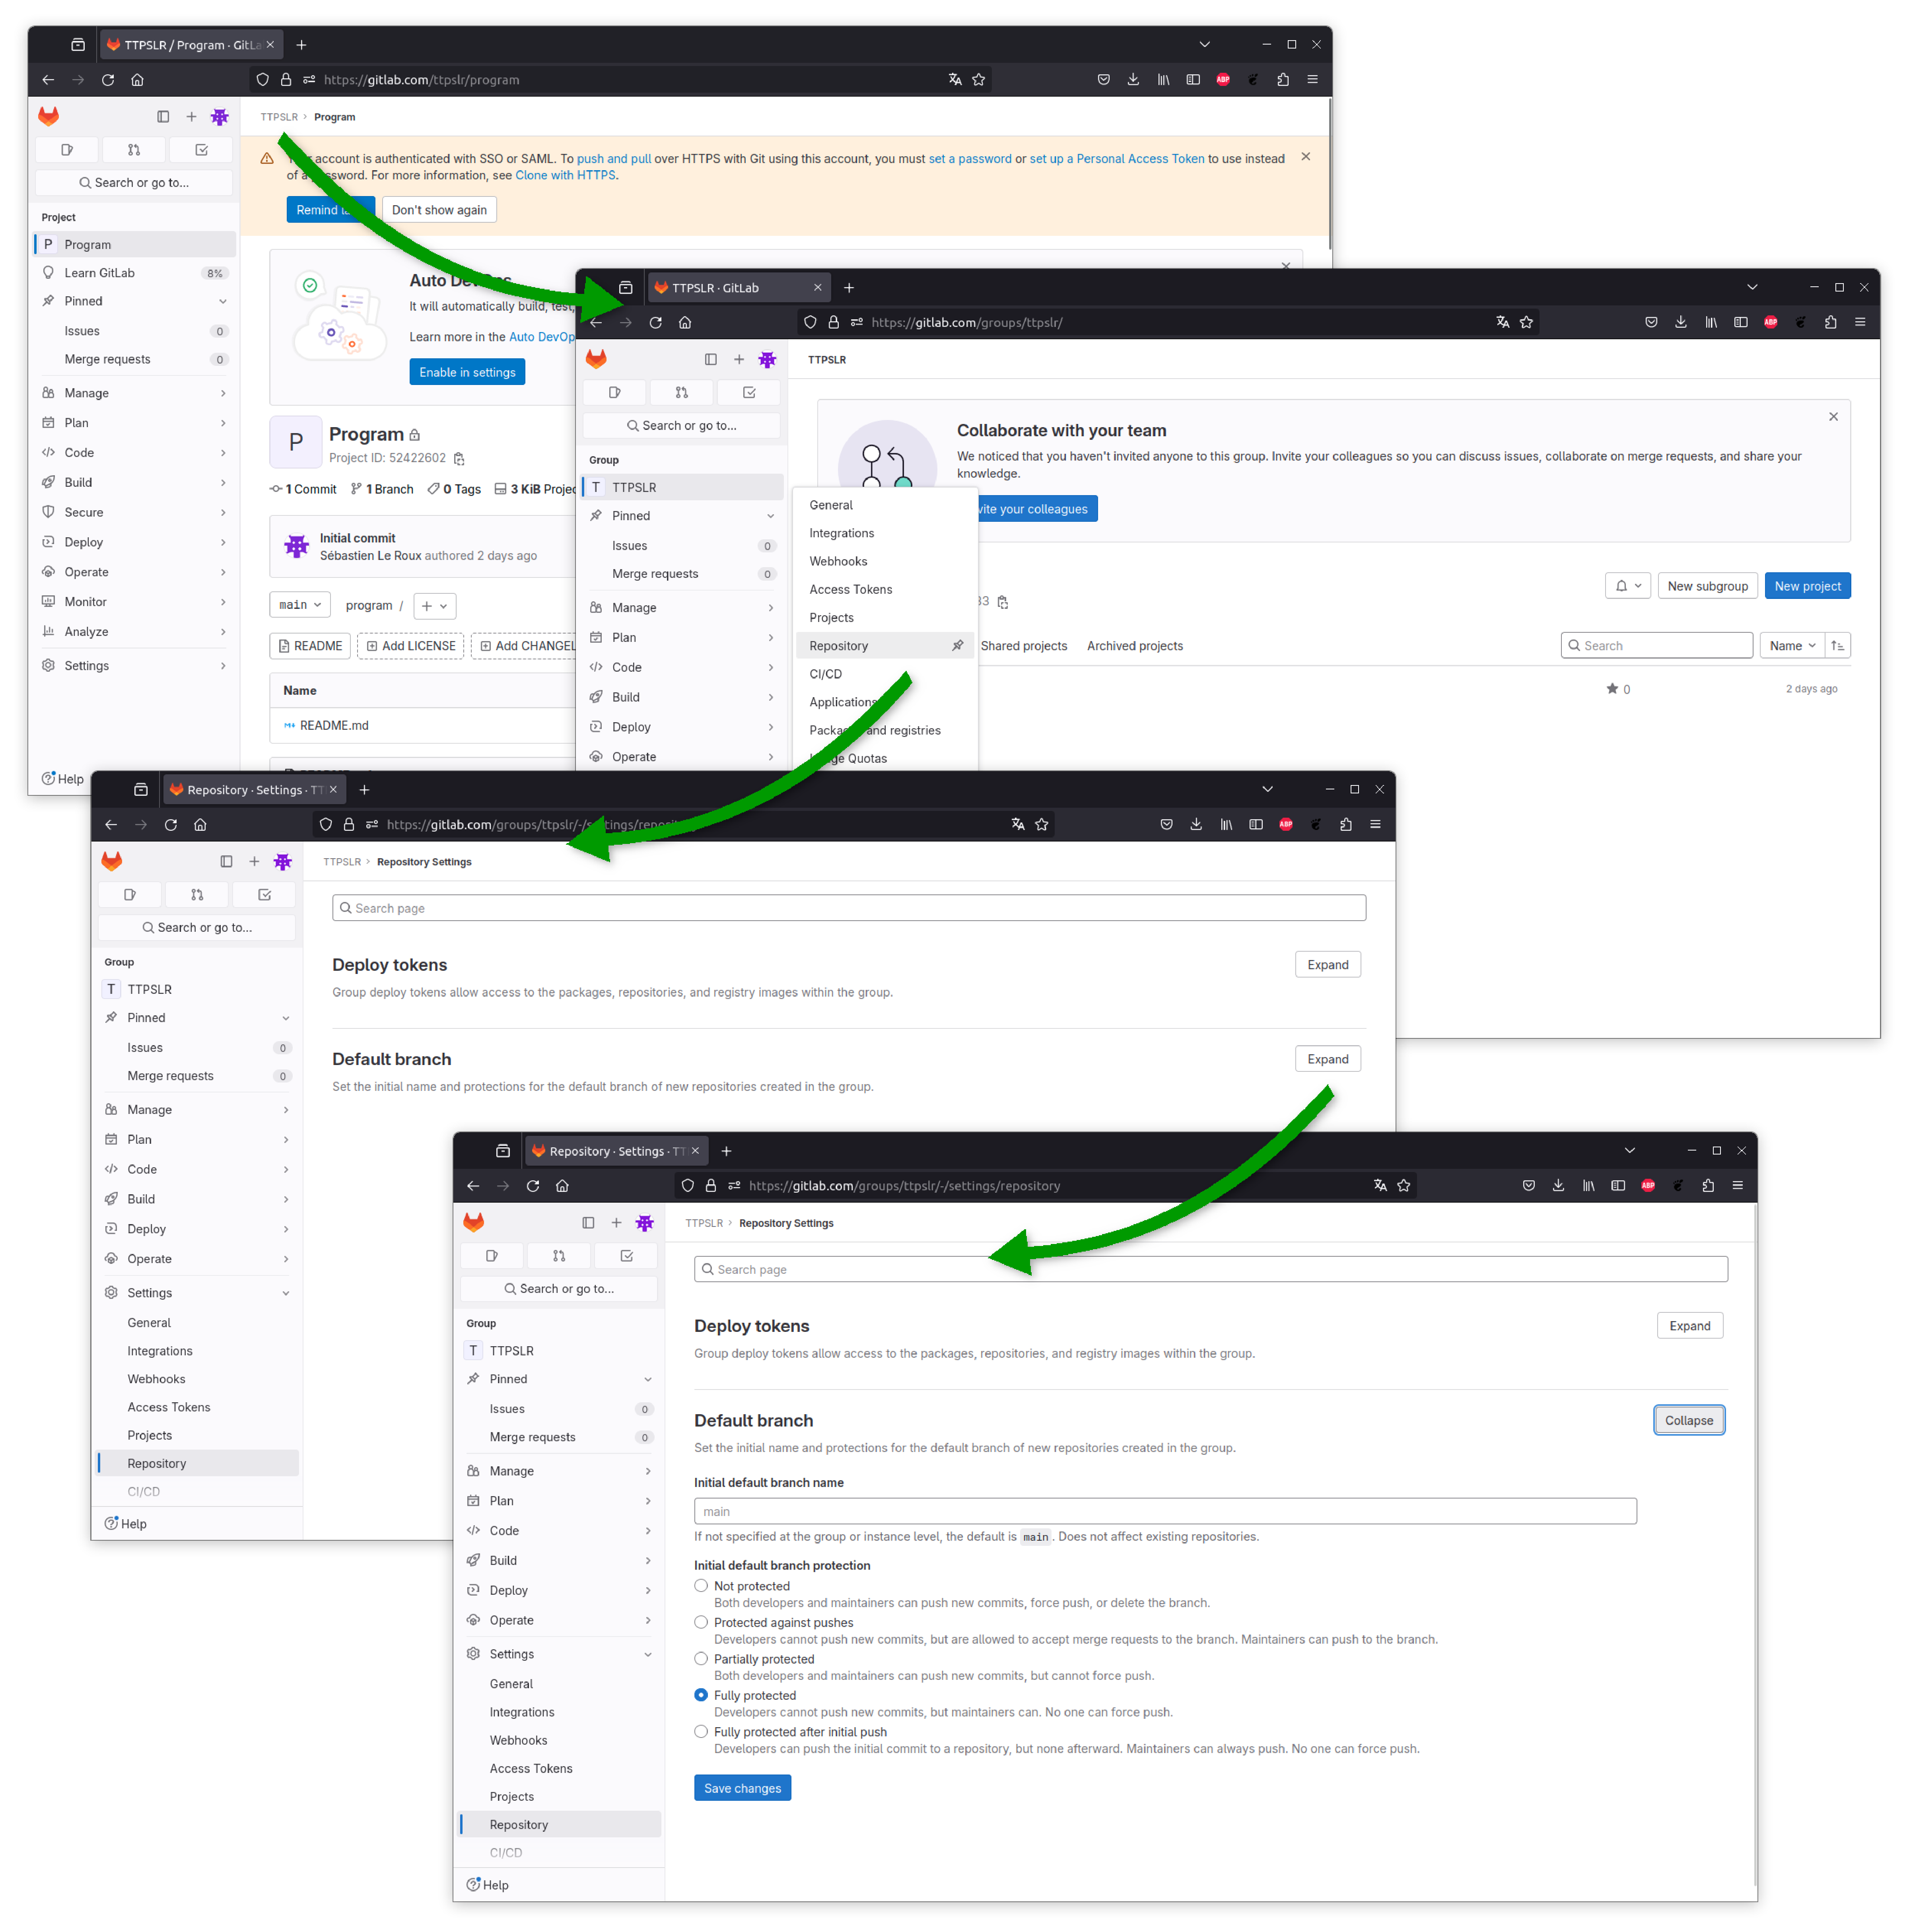
\includegraphics[width=1.0\textwidth,keepaspectratio=true,draft=\ddst]{img/hosts/gitlab/dbranch.eps} 
\caption{Default main branch projection on \gitlab\label{mbgitlab}}
\end{figure}

\begin{figure}[!p]
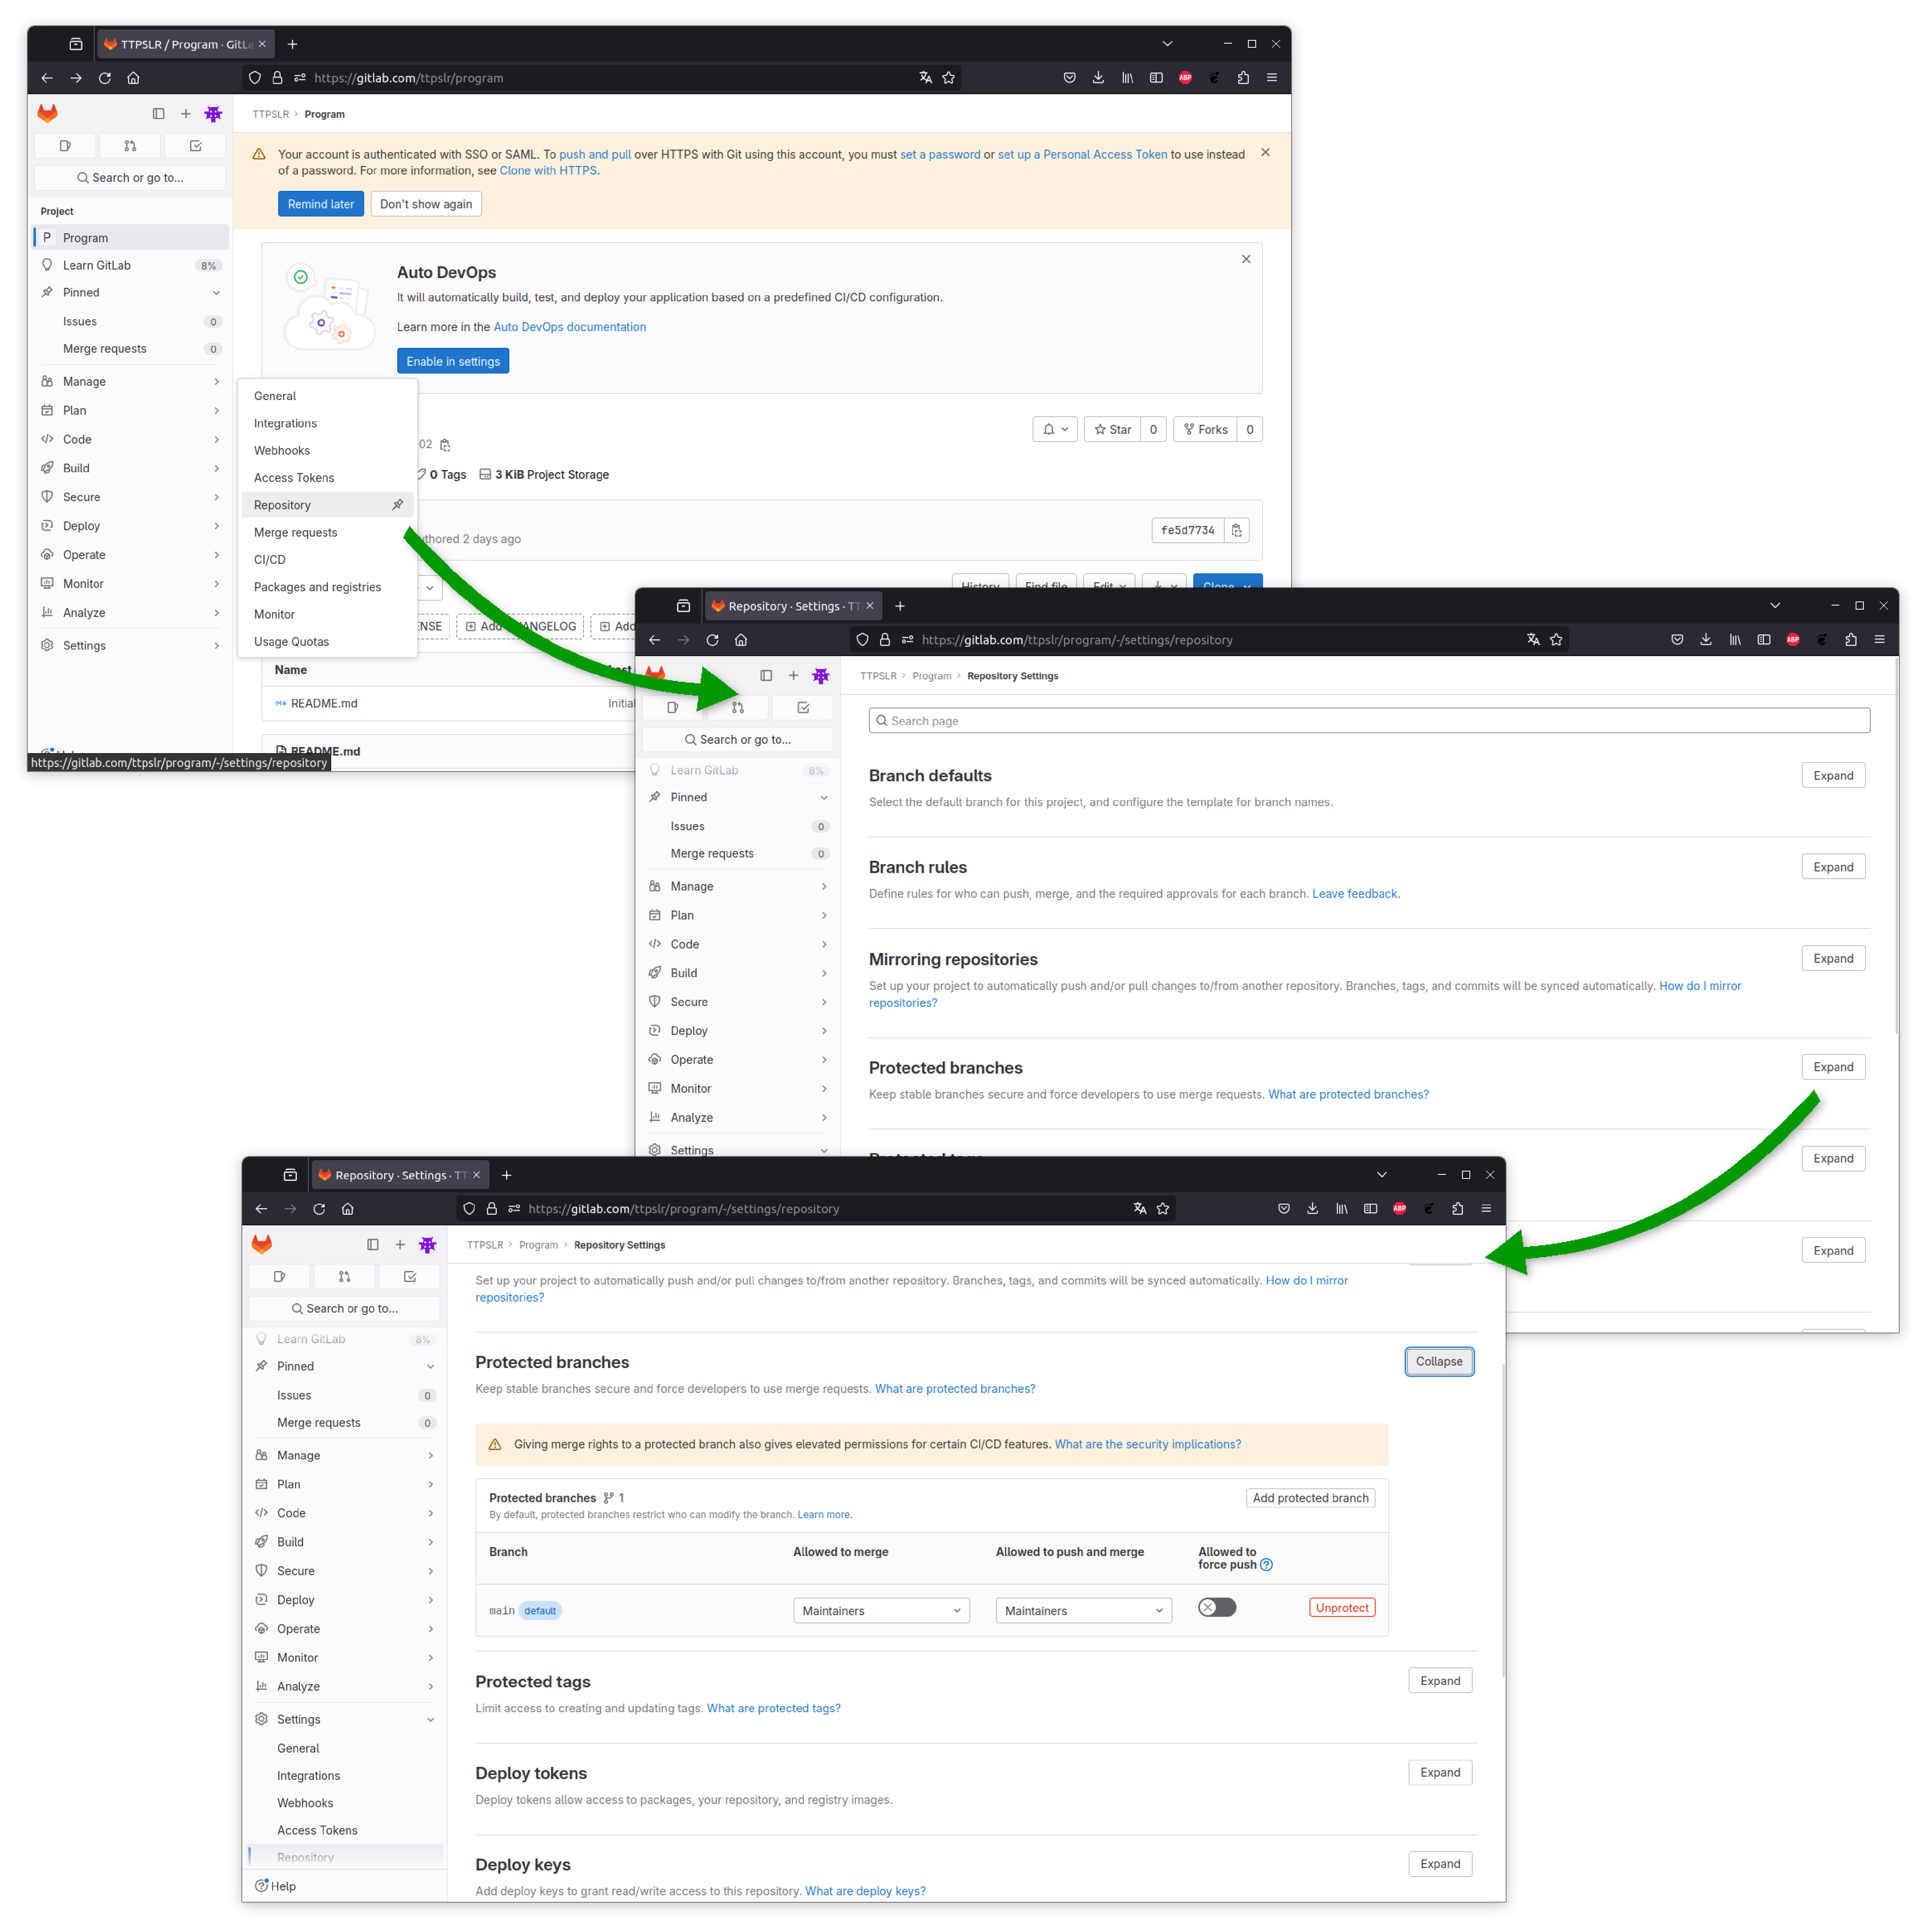
\includegraphics[width=1.0\textwidth,keepaspectratio=true,draft=\ddst]{img/hosts/gitlab/branch.eps} 
\caption{Project branch projection on \gitlab\label{bpgitlab}}
\end{figure}

\clearpage

\section{Releases and Tags}

\subsection{Tags}

On \github\ and \gitlab\ tags are images of the Git repository pointing towards archives that never change, 
like snapshots of the repository. \\
In both \github\ and \gitlab\ you can create tags whenever you think it is appropriate, 
however tags being required to produce a release, and a specific tag being associated with a specific release 
I will only focus thereafter in creating tag whenever creating release is required. 

\subsection{Releases}

On \github\ and \gitlab\ releases are deployable software versions made available for users to download. 
Releases are based on tags targeting specific points in the history of the repository. \\
To create a release: 
\begin{itemize}
\item On \github\ (see figure~\ref{rgithub}):
\begin{itemize}
\item Click on "\texttt{Create a new release}"
\item Click on "\bftt{Choose a tag}" to open the corresponding combo box:
\begin{itemize}
\item Input the new tag name, ex: "\texttt{1.0.0}" 
\item If the tag is new it is immediately proposed to create this tag
\item Click on "\bftt{Create new tag:} \bftt{1.0.0} \texttt{on publish}" \\
(or any other tag name of your choice)
\end{itemize}
\item Fill the description of the release, including release notes
\item Scroll down and click on "\texttt{Publish release}"
\end{itemize}
On \github\ releases packages have the form: "\rtt{tag}\bftt{.tar.gz}" \\
Extracting the archive on your hard drive will create a folder named: "\dgtt{repository-}\rtt{tag}"
\item On \gitlab\ (see figure~\ref{rgitlab}):
\begin{itemize}
\item On the left side menu, click on "\texttt{Deploy}" $\Longrightarrow$ "\texttt{Releases}"
\item Then click on "\texttt{Create a new release}"
\item Click on "\bftt{Tag name} \texttt{(required)}" to open the corresponding combo box:
\begin{itemize}
\item Input the new tag name, ex: "\texttt{1.0.0}" 
\item If the tag is new it is immediately proposed to create this tag
\item Click on "\texttt{Create tag} \bftt{1.0.0}" (or any other tag name of your choice)
\item Click on "\texttt{Save}"
\end{itemize}
\item Fill the description of the release, including release notes
\item Scroll down and click on "\texttt{Create release}"
\end{itemize}
On \gitlab\ releases packages have the form: "\dgtt{project}-\rtt{tag}\bftt{.tar.gz}" \\
Extracting the archive on your hard drive will create a folder named: "\dgtt{project-}\rtt{tag}"
\end{itemize}

\begin{figure}[!p]
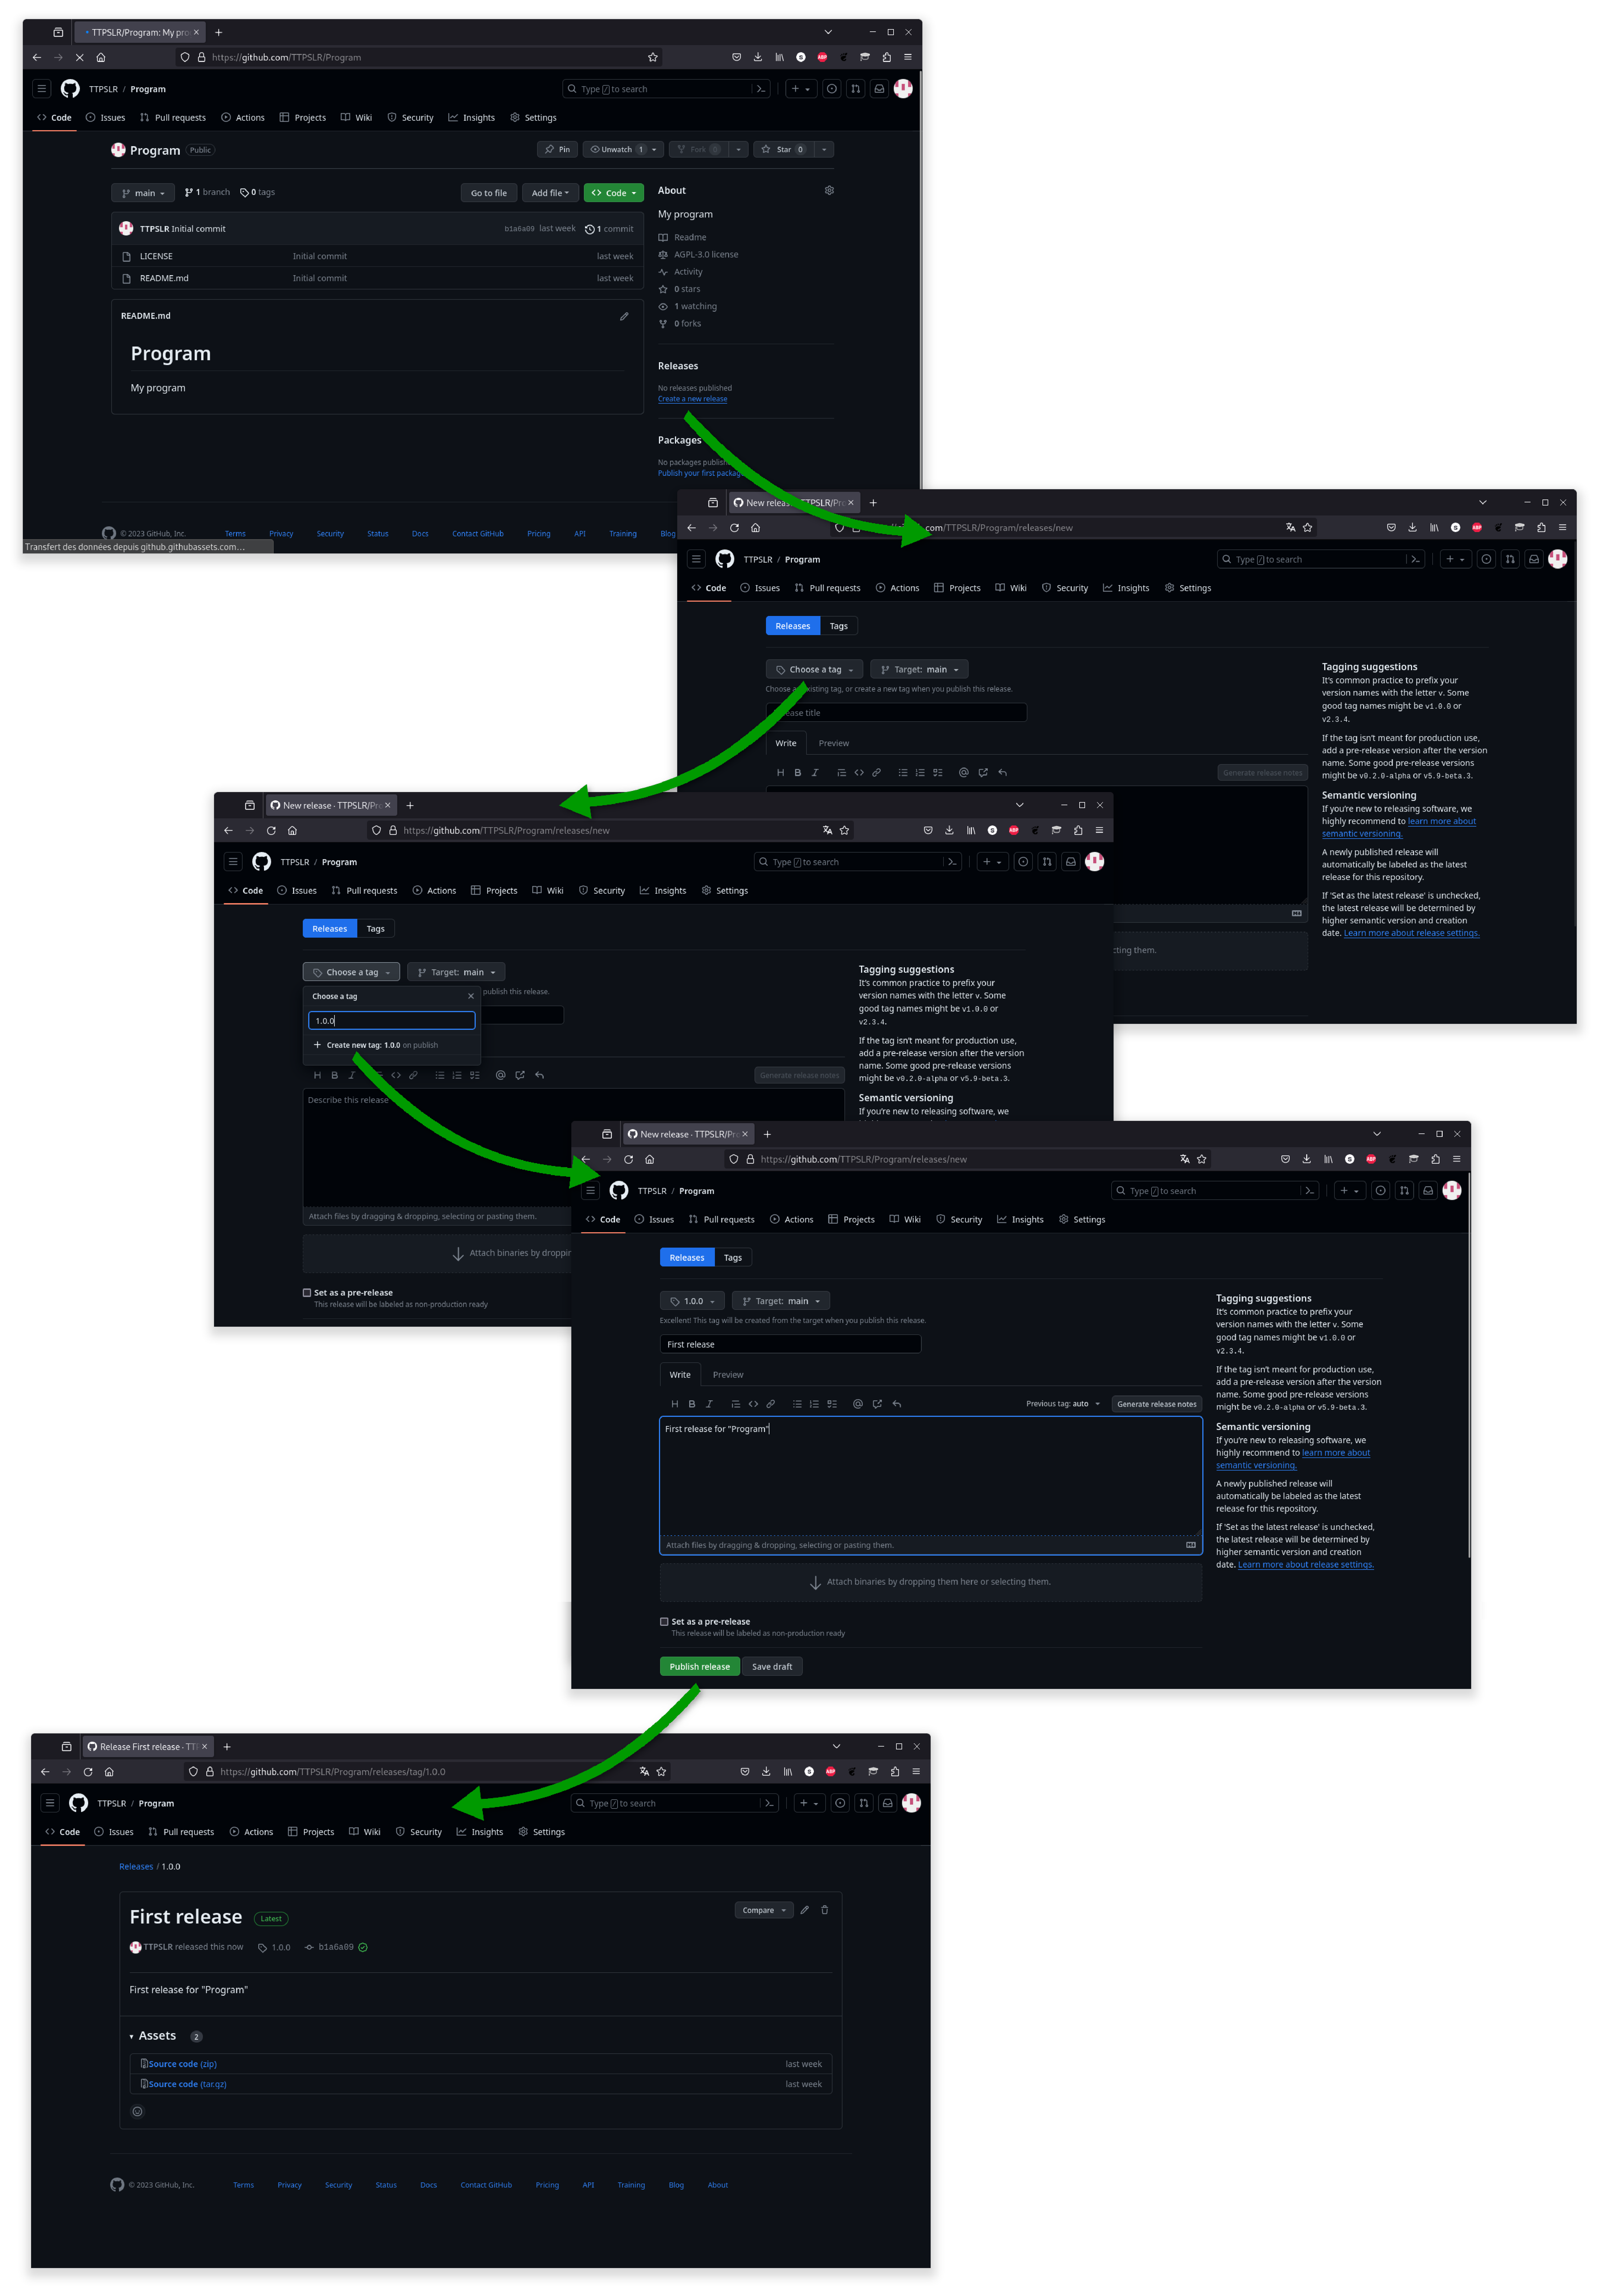
\includegraphics[width=1.0\textwidth,keepaspectratio=true,draft=\ddst]{img/hosts/github/release.eps} 
\caption{Creating a release on \github\label{rgithub}}
\end{figure}

\begin{figure}[!p]

\includegraphics[width=1.0\textwidth,keepaspectratio=true,draft=\ddst]{img/hosts/gitlab/release.eps} 
\caption{Creating a release on \gitlab\label{rgitlab}}
\end{figure}

\clearpage

\section{Using Git to manage your GitHub / GitLab project}
\label{onlinegit}

\subsection{Setting up work on you local computer} 

To start working on a remote repository using Git you can:
\begin{itemize}
\item {\bf{Clone}} the distant repository:
\begin{itemize}
\item \github:
{\footnotesize{
\begin{scriptii}
\fprompt{~/program} \bftt{git clone} git@github.com:\rtt{Author}/\btt{Program}
\end{scriptii}
}}
\item \gitlab:
{\footnotesize{
\begin{scriptii}
\fprompt{~/program} \bftt{git clone} git@gitlab.com:\rtt{Group}/\btt{Program}
\end{scriptii}
}}
\end{itemize}
\noindent Be careful \red{{\bf{NOT}}} to clone the distant repository using the "\texttt{https://git***}" instruction 
(both options being offered by \github\ and \gitlab), 
this would modify the access to the repository via the Git command line and require additional security considerations to setup 
developer access tokens, not considered in this manual. \\[0.25cm]
\item Alternatively set up manually the local folder to work remotely:
{\footnotesize{
\begin{scripti}
\fprompt{~} \bftt{mkdir} program
\fprompt{~} \bftt{cd} program
\fprompt{~/program} \bftt{git init}
\end{scripti}
}}
\begin{itemize}
\item \github:
{\notsofoot{
\begin{scriptii}
\fprompt{~/program} \bftt{git remote} add origin git@github.com:\rtt{Author}/\btt{Program}
\end{scriptii}
}}
\\[-0.75cm]
\noindent Replace:
\begin{itemize}
\item \rtt{Name}\quad by the GitHub account that owns the repository.
\item \btt{Program}\quad by the name of the repository. \\
\end{itemize}
\item \gitlab:
{\notsofoot{
\begin{scriptii}
\fprompt{~/program} \bftt{git remote} add origin git@gitlab.com:\rtt{Group}/\btt{Program}
\end{scriptii}
}}
\\[-0.75cm]
\noindent Replace:
\begin{itemize}
\item \rtt{Group}\quad by the group Id for the GitLab account that owns the project.
\item \btt{Program}\quad by the name of the project. \\
\end{itemize}
\end{itemize}
This should be enough to get you started, providing that you check that the git user name and email are set properly (see [Sec.~\ref{gitconfig}]). \\[0.25cm]
Finally if needed setup the user information:
{\footnotesize{
\begin{scripti}
\fprompt{~} \bftt{git} \rtt{config} user.name "\abtt{Your Name}"
\fprompt{~} \bftt{git} \rtt{config} user.email \dctt{\email}
\end{scripti}
}}
\\[-0.75cm]
\noindent Replace:
\begin{itemize}
\item \rtt{Your Name}\quad by your user name. 
\item \btt{\email}\quad by your email. \\
\end{itemize}
Update the local folder with the content of the remote repository:
{\footnotesize{
\begin{scripti}
\fprompt{~/program} \bftt{git pull} origin \rtt{branch}
\end{scripti}
}}
\\[-0.75cm]
\noindent Replace:
\begin{itemize}
\item \rtt{branch}\quad by the branch of the project your are working on. 
\end{itemize} 
\end{itemize}
When this is done you can verify the link between your local folder and the on-line repository using:
\begin{script}
\fprompt{~/program} \bftt{git} remote -v
origin	git@github.com:\rtt{Author}/\btt{Program} (fetch)
origin	git@github.com:\rtt{Author}/\btt{Program} (push)
\end{script}
\\[-0.5cm]
\noindent Where:
\begin{itemize}
\item \rtt{Author}\quad is the GitHub account that owns the repository.
\item \btt{Program}\quad is the name of the repository. 
\end{itemize}

\subsection{Contributing to other project(s) and collaborative work}

If you want to work on project hosted on \github\ or \gitlab, and that you are not managing the project you intend to work on, then you need first to {\bf{fork}} this project. 
That means to create your own personnal copy of this project, independent of the original repository. \\
Afterwards to submit your modification(s) to the main repository you will need to create a dedicated branch and request to merge your branch to the main project. 
Modification(s) will be checked by a project manager, and if appropriate will be merged to the main branch of the repository. \\[0.25cm]
To fork an exisiting project:
\begin{itemize}
\item On \github\ (see figure~\ref{fgithub}):
\begin{itemize}
\item Navigate to the \github\ project page of the repository you want to fork
\item Click on "\texttt{Fork}" to open the scrolling menu, and select "\texttt{Create a new fork}"
\item Follow the dialog to create a fork on the project in your own repository, you can select a specific branch if required, then when ready click on "\texttt{Create fork}"
\item It's done your own fork of the target project is now ready for you to work on in your own \github\ repository. 
\end{itemize}
\item On \gitlab\ (see figure~\ref{fgitlab}):

\end{itemize}

\newpage
\section{Project pages and documentation}

This section will illustrates how to use a \github\ / \gitlab\ repository and web pages to host a static web documentation for your project. 

\subsection{prerequisites}

It is required to install some tools to handle the publication of static webpages that will be used thereafter:
\begin{itemize}
\item Prepare the "\texttt{\textasciitilde/.bashrc}" file to install Ruby, insert the following lines:
\begin{scripti}
\fprompt{~} vi .bashrc
\comm{Install Ruby Gems to ~/gems}
\bad{export} \dctt{GEM\_HOME}\bad{=}\say{\$HOME/gems}
\bad{export} \dctt{PATH}\bad{=}\say{\$HOME/gems/bin:\$PATH}
\bad{export} \dctt{PATH}\bad{=}\say{\$HOME/.rbenv/bin:\$PATH}
\bftt{eval} \say{\$(rbenv init -)}
\bad{export} \dctt{PATH}\bad{=}\say{\$HOME/.rbenv/plugins/ruby-build/bin:\$PATH}
\end{scripti}
\item Install the Ruby dependencies (if needed)
\begin{itemize}
\item Fedora:
\vspace{-0.25cm}
{\footnotesize{
\begin{scriptii}
\textasciitilde]\$ \rtt{sudo} \bftt{dnf} install git-core gcc rust patch make bzip2 openssl-devel \textbackslash
                      libyaml-devel libffi-devel readline-devel zlib-devel \textbackslash
                      gdbm-devel ncurses-devel perl-FindBin perl-lib \textbackslash
                      perl-File-Compare
\end{scriptii}
}}
\item Debian:
\vspace{-0.25cm}
{\footnotesize{
\begin{scriptii}
\textasciitilde]\$ \rtt{sudo} \bftt{apt} install postgresql libpq-dev nodejs yarnpkg git zlib1g-dev \textbackslash
                      build-essential libssl-dev libreadline-dev libyaml-dev \textbackslash
                      libsqlite3-dev sqlite3 libxml2-dev libxslt1-dev \textbackslash
                      libcurl4-openssl-dev software-properties-common \textbackslash
                      libffi-dev
\end{scriptii}
}}
\end{itemize}
\item Install "\texttt{rbenv}":
{\footnotesize{
\begin{scripti}
\textasciitilde]\$ git clone https://github.com/rbenv/rbenv.git ~/.rbenv
\textasciitilde]\$ git clone https://github.com/rbenv/ruby-build.git ~/.rbenv/plugins/ruby-build
\textasciitilde]\$ \bftt{rbenv} \rtt{install} \dgtt{2.7.4}
\textasciitilde]\$ \bftt{rbenv} \rtt{global} \dgtt{2.7.4}
\textasciitilde]\$ \bftt{ruby} -v
\end{scripti}
}}
\\[-0.5cm]
\noindent \github\ pages are best compatible with version 2.7.x so do not install more recent release. \\
To list available stable versions:
{\footnotesize{
\begin{scripti}
\textasciitilde]\$ \bftt{rbenv} \rtt{install} \dctt{-l}
\end{scripti}
}}
\item Update "\texttt{rubygem}":
{\footnotesize{
\begin{scripti}
\textasciitilde]\$ \bftt{gem} \rtt{update} \dgtt{--system}
\end{scripti}
}}
\item Install \href{https://jekyllrb.com}{Jekyll} and the Ruby bundler:
\vspace{-0.25cm}
\begin{scripti}
\fprompt{~} \bftt{gem} \rtt{install} bundler jekyll
\end{scripti}
\end{itemize}
From this point forward the following steps are required to publish your documentation on \github\ or \gitlab\ pages:
\begin{enumerate}
\item Build the documentation of your project in \href{https://www.markdownguide.org/}{Markdown} and/or HTML language
\item Use Jekyll to convert your documentation in a static website
\item Create a repository on \github\ or \gitlab\ to host the documentation
\item Push your documentation to the web pages of the associated \github\ or \gitlab\ repository. 
\end{enumerate}

\subsection{Building the documentation in Markdown or HTML language}

It is up to you to decide how to do this, a good idea is to write your documentation in \LaTeX\ format, so that you can produce clean PDF documents. 
Then convert the \LaTeX\ files to HTML using \href{https://pandoc.org/}{pandoc}. \\
Also it allows to use your bibliography in Bib\TeX\ format and makes it easy to handle references on web pages. \\[0.25cm]
See the next section to know more about the data structure to prepare. \\[0.25cm]
Few things to take care of to use \LaTeX\ and \href{https://pandoc.org/}{pandoc} to prepare your documentation:
\begin{itemize}
\item To insert figures use PNG, or other graphic format, and not EPS as in standard \LaTeX\ documents. 
\item Be careful with the location of the images, ensure that the location, ideally in a separate and dedicated folder, 
matches the link in the HTML page. 
\item Internal references for objects not on the same HTML page will be lost when rendering the website. \\
This means that if your refer to a figure from the first chapter in the second chapter, likely on separate pages, 
you will have to correct the internal link to the proper web page. 
\item Pandoc conversion is not perfectly clean so few errors will likely require to be corrected afterwards, the best way 
to do that, is to understand the issue and to automate the correction process. \\
Among known errors to take care of:
\begin{itemize}
\item Check the table and figure captions
\item Some \LaTeX\ commands, in particular from peculiar custom packages, might not be understood by pandoc, and should be test proofed. \\[0.25cm]
For example the "\texttt{\textbackslash{Ctrl}}" command from the "\texttt{keystroke}" package (to render a drawing of the keyboard control key) 
cannot be processed by pandoc and should be replace by a command having the proper effect in HTML format, 
in this case "\texttt{\textbackslash{newcommand}\{\textbackslash{Ctrl}\}\{<kbd>Ctrl<\/kbd>\}}"
\end{itemize}
\item Finally to render \LaTeX\ math and equations in your HTML page insert the following code at the top of the HTML page:
\begin{itemize}
\item To render math using \href{https://www.mathjax.org/}{mathjax} use:
{\notsotiny{
\begin{scriptii}
\dbtt{<script} \abtt{src=}\red{"https://polyfill.io/v3/polyfill.min.js?features=es6"}\dbtt{></script>}
\dbtt{<script} \abtt{id=}\red{"MathJax-script" async src="https://cdn.jsdelivr.net/npm/mathjax@3.0.1/es5/tex-mml-chtml.js"}\dbtt{></script>}
\end{scriptii}
}}
\item To render math using \href{https://katex.org/}{katex} use:
{\notsotiny{
\begin{scriptii}
\dbtt{<script} \abtt{src=}\red{"https://cdnjs.cloudflare.com/ajax/libs/KaTeX/0.11.1/katex.min.js"}\dbtt{></script>}
\dbtt{<script>}document.addEventListener("DOMContentLoaded", function () {
   var mathElements = document.getElementsByClassName("math");
   var macros = [];
   for (var i = 0; i < mathElements.length; i++) {
      var texText = mathElements[i].firstChild;
      if (mathElements[i].tagName == "SPAN") {
       katex.render(texText.data, mathElements[i], {
        displayMode: mathElements[i].classList.contains('display'),
        throwOnError: false,
        macros: macros,
        fleqn: false
        });
      }}});
\dbtt{</script>}
\dbtt{<link} \abtt{rel=}\red{"stylesheet" href="https://cdnjs.cloudflare.com/ajax/libs/KaTeX/0.11.1/katex.min.css"} \dbtt{/>}
\dbtt{<!--}\abtt{[if lt IE 9]}\dbtt{>}
  \dbtt{<script} \abtt{src=}\red{"//cdnjs.cloudflare.com/ajax/libs/html5shiv/3.7.3/html5shiv-printshiv.min.js"}\dbtt{></script>}
\dbtt{<!}\abtt{[endif]}\dbtt{-->}
\end{scriptii}
}}
\end{itemize}
\end{itemize}
\vspace{-0.25cm}
Overall this method requires some additional work to properly convert the documents to a clean simple combination of Markdown and HTML structure, 
but once this work is automated you will only write your documentation using \LaTeX\ and then, in a single command, 
convert it and publish it to \github\ or \gitlab\ pages. 

\subsection{Using Jekyll to build a static website}

\href{https://jekyllrb.com}{Jekyll} is a simple static site generator. \\
Think of it like a file-based CMS, without all the complexity. Jekyll takes your content, renders Markdown and Liquid templates, 
and creates a complete, static website ready to be served by any web server. \\
Jekyll is the engine behind GitHub Pages, which you can use to host sites right from your GitHub repositories. \\[0.25cm]
Jekyll expects a document structure with Markdown files, but can also handles HTML files as includes files. 
In the following I will illustrate the document structure required by Jekyll to build a static web site: 
\begin{itemize}
\item For \LaTeX\ converted to HTML documentation
\item Using bibliography references in the \href{https://www.bibtex.org/}{Bib\TeX} format
\end{itemize}
Example repository to create the documentation: 
{\footnotesize{ 
\begin{script}
\fprompt{~/Program-doc} \bftt{ls}
\btt{\_bibliography}  \btt{chap-1}  \btt{intro}  \_config.yml  Gemfile  \btt{\_includes}  README.md
\end{script}
}}
\noindent With:
\begin{itemize}
\item Files:
\begin{itemize}
\item The home page of your documentation website: "\texttt{README.md}"
\item The list of Ruby extensions required to build your website: "\texttt{Gemfile}"
{\scriptsize{
\begin{scriptii}
\fprompt{~/Program-doc} \bftt{vi} Gemfile
source "\magenta{https://rubygems.org}"

\var{gem} '\magenta{jekyll-rtd-theme}'
\var{gem} '\magenta{github-pages}', \magenta{group}: :\magenta{jekyll\_plugins}
\var{gem} '\magenta{jekyll-scholar}', \magenta{group}: :\magenta{jekyll\_plugins}
group :\magenta{jekyll\_plugins} \bbtt{do}
  \var{gem} "\magenta{jekyll}", "\magenta{~> 3.9.0}"
  \var{gem} "\magenta{jekyll-feed}", "\magenta{~> 0.12}"
  \var{gem} "\magenta{jekyll-paginate}"
  \var{gem} "\magenta{jekyll-seo-tag}"
  \var{gem} "\magenta{jekyll-sitemap}"
  \var{gem} "\magenta{jekyll-archives}"
  \var{gem} "\magenta{jekyll-redirect-from}"
\bbtt{end}

\comm{Windows and JRuby does not include zoneinfo files,}
\comm{so bundle the tzinfo-data gem and associated library.}
platforms \magenta{:mingw}, \magenta{:x64\_mingw}, \magenta{:mswin}, \magenta{:jruby} \bbtt{do}
  \var{gem} "\magenta{tzinfo}", "\magenta{~> 1.2}"
  \var{gem} "\magenta{tzinfo-data}"
\bbtt{end}

\comm{ Performance-booster for watching directories on Windows}
\var{gem} "\magenta{wdm}", "\magenta{~> 0.1.1}", \magenta{:platforms} => [\magenta{:mingw}, \magenta{:x64\_mingw}, \magenta{:mswin}]
\end{scriptii}
}}
\item The Jekkyl configuration file to build the website: "\texttt{\_config.yml}"\\[-0.5cm] 
{\scriptsize{
\begin{scriptii}
\fprompt{~/Program-doc} \bftt{vi} \_config.yml
\var{title:} Program's documentation
\var{baseurl:} \magenta{"/Program-doc"}
\var{url:} \magenta{""}
\comm{GitHub or GtiLab repository:}
\var{repository:} TTPSLR/Program-doc
\var{lang:} en
\var{description:} This site presents the documentation for "Program"
\var{markdown:} kramdown
\var{highlighter:} rouge
\var{gist:}
  \var{noscript:} \magenta{false}
\var{kramdown:}
  \var{math\_engine:} mathjax
  \var{syntax\_highlighter:} rouge
\var{markdown\_extensions:}
  - \var{toc:}
    \var{permalink:} \magenta{"#"}
\comm{Define the depth of the menu}
    \var{baselevel:} 2
\var{banner:} \magenta{"/assets/img/banner.png"}
\var{favicon:} \magenta{"/assets/img/favicon.ico"}
\var{remote\_theme:} rundocs/jekyll-rtd-theme
\var{readme\_index:}
  \var{with\_frontmatter:} \magenta{true}

\var{plugins:}
  - jekyll-coffeescript
  - jekyll-default-layout
  - jekyll-gist
  - jekyll-github-metadata
  - jekyll-optional-front-matter
  - jekyll-paginate
  - jekyll-readme-index
  - jekyll-titles-from-headings
  - jekyll-relative-links
  - jekyll-scholar
  - jekyll-feed
  - jekyll-paginate
  - jekyll-seo-tag
  - jekyll-sitemap
  - jekyll-archives
  - jekyll-redirect-from
  - jekyll-remote-theme

\var{scholar:}
  \var{locale:} en
  \var{source:} ./\_bibliography
  \var{style:} \_bibliography/my-ieee.cls
  \var{bibliography:} references.bib
  \var{bibliography\_template:} \magenta{""}
  \var{replace\_strings:} \magenta{true}
  \var{join\_strings:}    \magenta{true}
  \var{use\_raw\_bibtex\_entry:} \magenta{false}
  \var{details\_dir:}    bibliography
  \var{details\_layout:} bibtex.html
  \var{details\_link:}   Details
\comm{Ensure that details are not printed twice}
  \var{query:} \magenta{"@*"}

\var{exclude:}
  - CNAME
  - Gemfile
  - Gemfile.lock
\end{scriptii}
}}
\end{itemize}
\item Directories:
\begin{itemize}
\item Each chapter or section in a separate directory, in this case "\btt{intro}" and "\btt{chap-1}":
\vspace{-0.25cm}
{\footnotesize{
\begin{scriptii}
\fprompt{~/program-doc} \bftt{ls} intro
README.md

\fprompt{~/program-doc} \lsr\ chap-1

chap-1:
README.md  \btt{section-1}  \btt{section-2}

chap-1/section-1:
README.md

chap-1/section-2:
README.md
\end{scriptii}
}}\\[-0.5cm]
\noindent Including sub-directories for chapter sections if required. \\
Note that each directory contains a single "\texttt{README.md}" file, dedicated to a single page of your site. \\[0.25cm]
\item Include files in the "\btt{\_includes}" directory:
{\footnotesize{
\begin{scriptii}
\fprompt{~/program-doc} \lsr\ \_includes
.:
\btt{intro}  \btt{chap-1}

./intro:
intro.html

./chap-1:
chap-1.html  \btt{section-1}  \btt{section-2}

./chap-1/section-1:
section-1.html

./chap-1/section-2:
section-2.html
\fprompt{~/program-doc}
\end{scriptii}
}} \\[-0.5cm]
\noindent including sub-directories for appendix chapters and sections if required. 
\newpage
\item The bibliography in the "\btt{\_bibliography}" directory:
{\footnotesize{
\begin{scriptii}
\fprompt{~/program-doc} \bftt{ls} \_bibliography
my-ieee.cls  references.bib
\end{scriptii}
}}
With:
\begin{itemize}
\item The "\texttt{*.ieee.cls}" file contains the bibliography style to apply
\item The "\texttt{*.bib}" file contains references in \href{https://www.bibtex.org/}{Bib\TeX} format \\
When you convert \LaTeX\ to HTML the keywords for the bibliography remain in the HTML document.
\end{itemize}
\end{itemize}
\end{itemize}
The "\texttt{README.md}" files, in Markdown format, follow the structure: 
{\footnotesize{
\begin{script}
\fprompt{~/program-doc} \bftt{vi} chap-1/README.md
\mdcom{This is a HTML comment in Markdown}
\mdcom{It will show up in the converted HTML document}

---
\mdcom{Position of this file in the website menu.}
\mdcom{To be compared will all other README.md file(s) at the same level,}
\mdcom{in this case all "~/program-doc/*/README.md" files}
sort: 2
\mdcom{Creation date:}
date: 2023-11-26
\mdcom{Math formula on this pages ?}
\mdcom{This is used to enable math javascript:}
maths: 1
---

\mdcom{# is the Markdown command for a heading}
\mdcom{Therefore the next line is the title of the chapter}
\magenta{# How to use "Program"}
\mdcom{Note if you do that you need to remove the heading line}
\mdcom{from the included HTML file bellow:}

\mdcom{Jekyll instruction to read an include file,}
\mdcom{and search for corresponding file(s) in the "\_include" folder}
\{\% include chap-1/chap-1.html \%\}

\mdcom{Jekyll instruction to process all sub-directories, if any:}
\{\% include list.liquid all=true \%\}

\mdcom{Jekyll instruction to add a bibliography section on this page:}
\{\% bibliography --cited \%\}
\mdcom{Then Jekyll search the "\_bibliography" folder to insert references}
\end{script}
}}
\clearpage
\noindent Jekyll will search for all "\texttt{README.md}" files in the directory tree, starting from the top directory. 
and build the website according to the "\texttt{sort}" instructions, in this example:
\begin{itemize}
\item Top level, homepage: "\texttt{README.md}"
\begin{itemize}
\item First level: \\
\begin{itemize}
\item In "\texttt{intro\textbackslash README.md}"  \,\,\ \quad$\Longrightarrow$\quad "\texttt{sort: }\rtt{1}"\\
\item In "\texttt{chap-\rtt{1}\textbackslash README.md}" \quad$\Longrightarrow$\quad "\texttt{sort: }\rtt{2}"\\
\item[$-$] Second level (chapter sections): \\
\begin{itemize}
\item In "\texttt{chap-1\textbackslash section-\rtt{1}\textbackslash README.md}" \quad$\Longrightarrow$\quad "\texttt{sort: }\rtt{1}"\\
\item In "\texttt{chap-1\textbackslash section-\rtt{2}\textbackslash README.md}" \quad$\Longrightarrow$\quad "\texttt{sort: }\rtt{2}"\\
\end{itemize}
\end{itemize}
\end{itemize}
\end{itemize}
Jekyll will create a HTML page for each "\texttt{README.md}" file found in the directory tree. \\
For your documentation to be easy to browse and read take time to organize it properly and split the pages accordingly. \\
The directories "\texttt{\_includes}" and "\texttt{\_bibliography}" are ignored by Jekyll when searching for "\texttt{README.md}" files, 
however their content is used to produce the website. \\[0.25cm]
To install the packages required by the "\texttt{Gemfile}" to build your site use:
\begin{script}
\fprompt{~/Program-doc} \bftt{bundle} \rtt{install}
\end{script}\\[-0.75cm]
\noindent Then to build the site use:
\begin{script}
\fprompt{~/Program-doc} \bftt{bundle} \rtt{exec} \dgtt{jekyll} build
\end{script}\\[-0.75cm]
\noindent You will see that this command creates a new directory name "\texttt{\_site}" that contains your website. 
\begin{script}
\fprompt{~/Program-doc} ls \_site

\end{script}\\[-0.75cm]
\noindent You can give a try to this website on your computer using: 
\begin{script}
\fprompt{~/Program-doc} \bftt{bundle} \rtt{exec} \dgtt{jekyll} serve
\end{script}\\[-0.75cm]
\noindent And simply follow the instructions.
\newpage

\subsection{Hosting the website on GitHub}

To use \github\ to host your documentation: 
\begin{itemize}
\item Create a dedicated repository, in the following example: "\texttt{TTPSLR/Program-doc}"
\item After properly configuring the connection to the remote repository, upload the contents of the "\texttt{\textasciitilde/Program-doc}" but the folder "\texttt{\_site}" to the main branch, separate branches allows to keep track of both the source material and the final content of the website:
\begin{scriptii}
\fprompt{~/Program-doc} \bftt{mv} \_site ../
\fprompt{~/Program-doc} \bftt{git} \rtt{checkout} \btt{-b} Main
\fprompt{~/Program-doc} \bftt{git} \rtt{add} .
\fprompt{~/Program-doc} \bftt{git} \rtt{commit} \btt{-m} "To build the doc"
\fprompt{~/Program-doc} \bftt{git} \rtt{push} \btt{origin} Main
\end{scriptii}
\item After properly configuring the connection to the remote repository, upload the contents of the "\texttt{\_site}" to the \github\ pages, the "\texttt{gh-pages}" branch:
\begin{scripti}
\fprompt{~/\_site} \bftt{git} \rtt{checkout} \btt{-b} gh-pages
\fprompt{~/\_site} \bftt{git} \rtt{add} .
\fprompt{~/\_site} \bftt{git} \rtt{commit} \btt{-m} "Documentation"
\fprompt{~/\_site} \bftt{git} \rtt{push} \btt{origin} gh-pages
\end{scripti}
\end{itemize}
After a short while the result is updated, and as is illustrated on figure~\ref{dgithub}, the website is alive. \\
Open the "\texttt{Pages}" tab in the "\texttt{Settings}" menu, to find out the web address of your site. \\
In this example: \href{https://ttpslr.github.io/Program-doc}{https://ttpslr.github.io/Program-doc} \\[0.25cm]
The \github\ pages address have the form:\quad https://\rtt{Author}.github.io/\btt{Program}

\begin{figure}[!p]
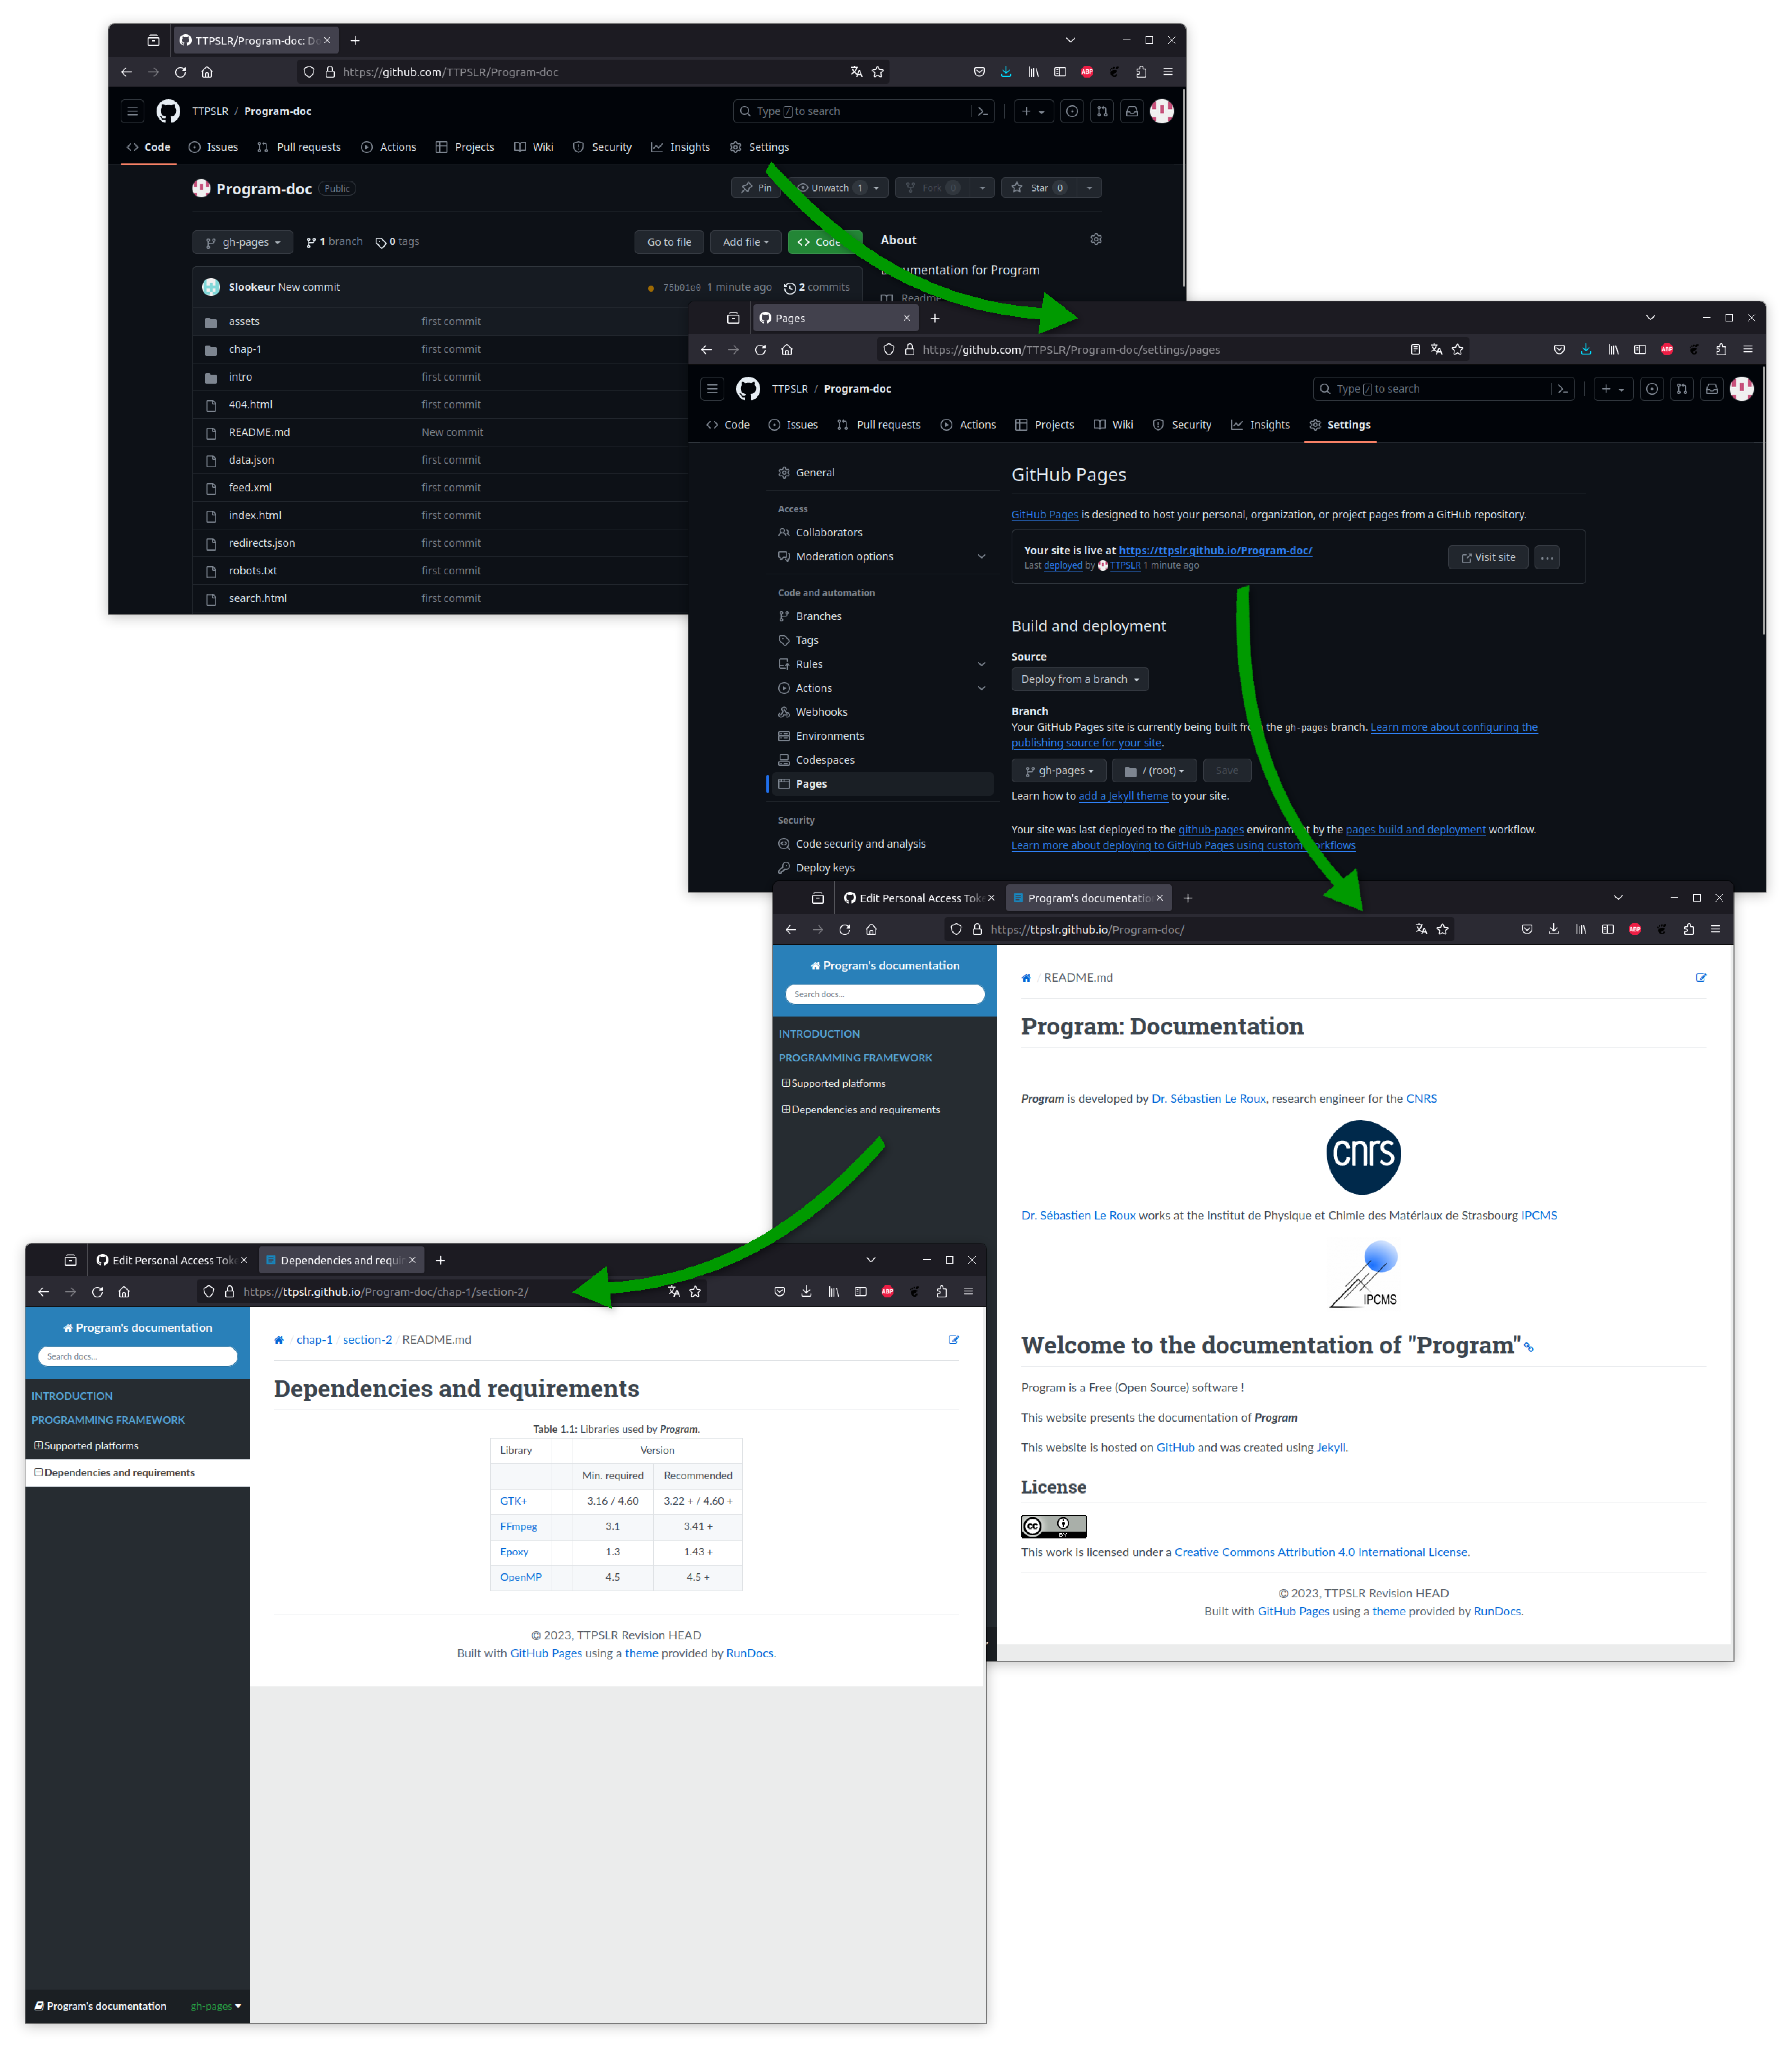
\includegraphics[width=1.0\textwidth,keepaspectratio=true,draft=\ddst]{img/hosts/github/doc.eps} 
\caption{Hosting the documentation on \github\label{dgithub}}
\end{figure}


\chapter{Linux distribution}

In the Linux world two distributions became widely famous, mostly because of the package distribution systems they implemented: 
\begin{itemize}
\item The \href{https://www.redhat.com}{Red Hat Linux} distribution that created and maintain the \href{https://en.wikipedia.org/wiki/RPM\_Package\_Manager}{RPM Package-Manager} "Red Hat Package Manager" system, that handles the installation/removal of \href{RPM "Red Hat Packages"}, files with the \bftt{.rpm} extension.
\item The \href{https://www.debian.org}{Debian Linux} distribution that created and maintain the \href{https://en.wikipedia.org/wiki/Dpkg}{dpkg} package management system, that handles the installation/removal of \href{https://en.wikipedia.org/wiki/Deb\_(file\_format)}{DEB "Debian Packages"}, files with \bftt{{.deb}} extension.
\end{itemize}
In 2023 there are thousands of Linux distributions, most of them are either Red Hat based and integrate the RPM Package-Manager, or, Debian based and integrate the dpkg package management system. \\
Integrating the package management systems of both Red Hat and Debian distributions is the most natural way to efficiently distribute your program to the entire open source / Linux community. \\
In the next sections I will review the requirements to achieve it providing that you already built a proper GNU tarball, or for that matter that you are already using any other build system. 
\clearpage

\section{RPM}

I the next pages I will introduce the proper way to build a RPM file suitable to be distributed by \href{https://www.fedora.org}{Fedora Linux} 
which is the upstream source for Red Hat Enterprise Linux. \\[0.25cm]
Maybe more importantly I will assume that you are working on Fedora Linux, 
that would make a lot of sense since we are talking about building Fedora RPMs here. 
Some of the commands I will use thereafter can only be found on Fedora, 
therefore I would recommend to download and install \href{https://getfedora.org/fr/workstation/download/}{the latest Fedora version} either on your computer or in a virtual machine. \\[0.5cm]
To prepare a RPM file you need first to install the appropriate tools: 
\begin{script}
\fprompt{~} sudo dnf install fedora-packager fedpkg rpmdevtools
\end{script}
\\[-0.5cm]
\noindent If I intend to provide tips and trick to help you prepare your RPM, I strongly recommend that you give a look to:
\begin{itemize}
\item The \href{https://rpm-packaging-guide.github.io/}{RPM Packaging Guide}.
\item The official \href{https://docs.fedoraproject.org/en-US/packaging-guidelines/}{Fedora packaging guidelines}. 
\item The \href{https://docs.fedoraproject.org/en-US/packaging-guidelines/}{Fedora packaging tutorial}.
\end{itemize}
Indeed this guide is not meant to be a thorough review of RPM packaging,  
that is actually much more complicated than for the simple desktop application used afterward to illustrate the process. 

\subsection{The "\bftt{.spec}" file}

The "\bftt{.spec}" file is a fundamental element in the packaging workflow. 
This file can be thought of as the "recipe" that the rpmbuild utility uses to actually build an RPM. 
It tells the build system what to do by defining instructions in a series of sections. \\
The next pages will introduce the basics required to create a simple "\bftt{.spec}" file, 
the complete example is provided in appendix~\ref{spec}. \\[0.25cm]
Please consider that each section of the "\bftt{.spec}" file as detailed between sections~\ref{rpminit}] and \ref{rpmlog} 
can be completed by your own set of specific instructions. \\[0.25cm] 
\noindent To create a new "\bftt{.spec}" file, use:
\begin{script}
\fprompt{~} rpmdev-newspec program
\end{script}
\clearpage
\noindent This will create a ready to be filled "\bftt{program.spec}" file: 
{\footnotesize{
\begin{script}
\comm{Initialization section - see [Sec.~\ref{rpminit}].}
\bad{Name:}           program
\bad{Version:}
\bad{Release:}        1\%{?dist}
\bad{Summary:}
\bad{License:}
\bad{URL:}
\bad{Source0:}

\comm{Information section - see [Sec.~\ref{rpminfo}].}
\bad{Provides:}

\dgtt{\%description}

\comm{Requirement sections - see [Sec.~\ref{rpmreq}].}
\bad{BuildRequires:}
\bad{Requires:}

\comm{Preparation to build section - see [Sec.~\ref{rpmprep}].}
\dgtt{\%prep}
\%autosetup

\comm{Build instructions section - see [Sec.~\ref{rpmbuild}].}
\dgtt{\%build}
\%configure
\%make\_build

\comm{Install instructions section - see [Sec.~\ref{rpminst}].}
\dgtt{\%install}
\%make\_install

\comm{Post-installation Linux integration section - see [Sec.~\ref{rpmpost}].}
\dgtt{\%check}

\comm{Package file paths section - see [Sec.~\ref{rpmfiles}].}
\dgtt{\%files}
\%license add-license-file-here
\%doc add-docs-here

\comm{ChangeLog section - see [Sec.~\ref{rpmlog}].}
\dgtt{\%changelog}
* \red{Wed Mar 29 2023} Your Name \blue{<\email>}
- 
\end{script}
}}
\\
\noindent In the next pages we will browse and complete this file section by section.

\clearpage
\subsubsection{Initialization section}
\label{rpminit}
\vspace{-0.75cm}
{\footnotesize{
\begin{script}
\comm{In a spec file, commented lines:}
\comm{\tabul Start by the \# symbol.}
\comm{\tabul When commenting a \% symbol, require to double it using another \%.}
\comm{Ex: This line is a commented line, \%\%\{Name\} is the first variable defined bellow.}

\comm{The name of the package, \bftt{MUST} be identical to the prefix name of the ".spec" file:}
\bad{Name:}      program
\comm{Optional, to define a variable using the \bftt{\%\%global} instruction.}
\comm{A variable \bftt{upname} is created, and used bellow as the name of the GitHub repository,}
\bftt{\%global} \var{upname} Program
\comm{Version of the program:}
\bad{Version:}   1.2.12
\comm{Release number of the RPM package, independent of the program's version.}
\comm{\tabul- Each time you provide a new release of program set this value to 1}
\comm{\tabul- Each time you modify something else in the package increment this number.}
\comm{Here the value is set to 3, meaning that it is the second modification}
\comm{of the package since release of version 1.2.12 of the program.}
\comm{\%\{?dist\} is a mandatory Fedora tag: .fc37, .fc38 ...}
\bad{Release:}   3\var{\%\{?dist\}}
\comm{Summary information about the program:}
\bad{Summary:}   An nice program
\comm{License information, should use the SPDX identifier, more information here:}
\comm{\tabul \href{https://spdx.org/licenses/}{https://spdx.org/licenses/}}
\comm{\tabul \href{https://docs.fedoraproject.org/en-US/legal/license-field/}{https://docs.fedoraproject.org/en-US/legal/license-field/}}
\bad{License:}   AGPL-3.0-or-later
\comm{Source tarball that uses a known build system.}
\comm{GitHub repository of the program, specify the archive to download using its tag:}
\comm{In this example the GitHub tag is "v1.2.12"}
\bad{Source0:}   \gitauth/\var{\%\{upname\}}/archive/refs/tags/v\var{\%\{version\}}.tar.gz
\comm{To sign the RPM package with a GPG key uncomment the next 2 lines:}
\comm{Source1:   ./v\%\%\{version\}.tar.gz.asc}
\comm{Source2:   \%\%\{name\}.gpg}
\comm{The webpage of the project:}
\bad{URL:}        https://www.\var{\%\{name\}}.com/
\end{script}
}}
\vspace{-0.5cm}

\subsubsection{Information section}
\label{rpminfo}
\vspace{-0.75cm}
{\footnotesize{
\begin{script}
\comm{Optional, to inform the package manager about your package.}
\comm{This allows your package to be required by another one,}
\comm{using the \bftt{Requires:} instruction - see [Sec.~\ref{rpmreq}]}
\bad{Provides:} \var{\%\{name\}} = \var{\%\{version\}}-\var{\%\{release\}}

\comm{A short description of the program capabilities, up to the next \%:}
\dgtt{\%description}
This program is amazing: 
- It uses GTK3 for the graphical user interface.
- It uses OpenGL to render 3D stuff
- It uses FFMPEG to encode videos
\end{script}
}}

\subsubsection{Requirement sections}
\label{rpmreq}

This section regroups requirements, to build and to run the program:
{\footnotesize{
\begin{script}
\comm{To set a requirement to build the program use the \bftt{BuildRequires:} instruction:}

\comm{If the GNU Autotools are required to build it:}
\bad{BuildRequires:} make
\bad{BuildRequires:} automake
\bad{BuildRequires:} autoconf
\end{script}
}}
\vspace{-0.75cm}
{\footnotesize{
\begin{script}
\comm{If CMake is required to build it:}
\bad{BuildRequires:} cmake
\end{script}
}}
\vspace{-0.75cm}
{\footnotesize{
\begin{script}
\comm{If meson is required to build it:}
\bad{BuildRequires:} meson
\end{script}
}}
\vspace{-0.75cm}
{\footnotesize{
\begin{script}
\bad{BuildRequires:} pkgconf-pkg-config
\bad{BuildRequires:} gcc
\bad{BuildRequires:} gcc-gfortran
\bad{BuildRequires:} libgfortran

\comm{Library required to build the program, test performed by pkgconf}
\bad{BuildRequires:} pkgconfig(gtk+-3.0)
\bad{BuildRequires:} pkgconfig(libxml-2.0)
\bad{BuildRequires:} pkgconfig(glu)
\bad{BuildRequires:} pkgconfig(epoxy)
\bad{BuildRequires:} pkgconfig(libavutil)
\bad{BuildRequires:} pkgconfig(libavcodec)
\bad{BuildRequires:} pkgconfig(libavformat)
\bad{BuildRequires:} pkgconfig(libswscale)

\comm{Requirements for \href{https://www.freedesktop.org/wiki/}{FreeDesktop} integration - see [Sec.~\ref{rpmpost}]:}
\bad{BuildRequires:} desktop-file-utils
\bad{BuildRequires:} libappstream-glib

\comm{To sign the RPM package with a GPG key uncomment the next line:} 
\comm{BuildRequires: gnupg2}

\comm{To set a requirement to run the program use the \bftt{Requires:} instruction:}
\comm{Requirements, packages that are needed, at runtime.}
\comm{The only ways to be sure what to add here: }
\comm{- Use \bftt{rpmlint} to verify your rpm after the build - see [Sec.~\ref{rpmtesting}]}
\comm{- Try installing your RPM on a clean system.}
\bad{Requires:} gtk3
\bad{Requires:} mesa-libGLU
\end{script}
}}

\clearpage
\subsubsection{Preparation section}
\label{rpmprep}
This section prepare everything required to build the package, not only the program itself.
{\footnotesize{
\begin{script}
\dgtt{\%prep}
\comm{To sign the RPM package with a GPG key uncomment the next line:}
\comm{\%\%\{gpgverify\} --keyring={\textquotesingle}\%\%\{SOURCE2\}{\textquotesingle} --signature={\textquotesingle}\%\%\{SOURCE1\}{\textquotesingle} --data={\textquotesingle}\%\%\{SOURCE0\}{\textquotesingle}}

\comm{Preparing the build.}
\comm{The \bftt{autosetup} instruction automates the setup process.}
\comm{The "-n" option specifies the name of the folder created}
\comm{by extracting the GNU tarball:}
\bftt{\%autosetup} \rtt{-n} \var{\%\{upname\}}-\var{\%\{version\}}
\comm{Note that \bftt{autosetup} is independent of the build system.}
\comm{For information regarding options:}
\comm{\href{https://rpm-software-management.github.io/rpm/manual/autosetup.html}{https://rpm-software-management.github.io/rpm/manual/autosetup.html}}
\end{script}
}}

\vspace{-0.25cm}
\subsubsection{Build instructions section}
\label{rpmbuild}

This section describes the instructions requires to build the program. 
{\footnotesize{
\begin{script}
\comm{With the GNU Autotools:}
\dgtt{\%build}
\comm{The first step is to call the \bftt{configure} script:}
\bftt{\%configure}
\comm{Then build the program using the \bftt{make} command:}
\bftt{\%make\_build}
\comm{This will force to use parallel building.}
\comm{If you want to adjust the number of CPU cores, use:}
\comm{\%\%make \%\%{smp\_mflags -j20}}
\end{script}
}}
\vspace{-0.75cm}
{\footnotesize{
\begin{script}
\comm{With CMake:}
\dgtt{\%build}
\comm{To configure use:}
\bftt{\%cmake}
\comm{Then to build use:}
\bftt{\%cmake\_build}
\comm{This will force to use parallel building.}
\end{script}
}}
\vspace{-0.75cm}
{\footnotesize{
\begin{script}
\comm{With meson:}
\dgtt{\%build}
\comm{To configure use:}
\bftt{\%meson}
\comm{Then to build use:}
\bftt{\%meson\_build}
\comm{This will force to use parallel building.}
\end{script}
}}

\vspace{-0.25cm}
\subsubsection{Install instructions section}
\label{rpminst}

This section describes the instructions requires to install the program. 
{\footnotesize{
\begin{script}
\comm{With the GNU Autotools:}
\dgtt{\%install}
\comm{Install the program using the \bftt{make} command:}
\bftt{\%make\_install}
\end{script}
}}
\vspace{-1cm}
{\footnotesize{
\begin{script}
\comm{With CMake:}
\dgtt{\%install}
\comm{Install the program using:}
\bftt{\%cmake\_install}
\end{script}
}}
\vspace{-1cm}
{\footnotesize{
\begin{script}
\comm{With meson:}
\dgtt{\%install}
\comm{Install the program using:}
\bftt{\%meson\_install}
\end{script}
}}


\subsubsection{Post-installation Linux and FreeDesktop integration section}
\label{rpmpost}

The \bftt{check} section allows to input commands required after the installation process. \\
If your are building an application then 2 files must be delivered with your package:
\begin{itemize}
\item The custom MIME association "\bftt{-mime.xml}" file \\[0.25cm]
\href{https://help.gnome.org/admin/system-admin-guide/stable/mime-types.html.en}{MIME types} are used to create and define file association(s) with a program. \\ 
An example of custom MIME association file is provided in the appendix~\ref{mime}.
\item The desktop entry or "\bftt{.desktop}" file \\[0.25cm]
\href{https://specifications.freedesktop.org/desktop-entry-spec/latest/}{Desktop entries} are desktop configuration files describing 
how a particular program is to be launched, how it appears in menus, etc. \\
An example of desktop entry for a desktop application is provided in the appendix~\ref{desktop}.
\item The AppStream metadata or "\bftt{.appdata.xml}" file \\[0.25cm]
\href{https://www.freedesktop.org/software/appstream/docs/}{AppStream metadata} allows upstream projects to define metadata 
about the components they provide using small XML files, metainfo files, which get installed into locations on the client system 
and are used by distributors to enhance their metadata. \\ 
The name of this file should follow the structure:
\vspace{-0.125cm}
\begin{center}\btt{web.adress.reversed}\rtt{.}\bftt{appdata.xml}\end{center}
\vspace{-0.25cm}
\begin{itemize}
\item The website of the program is: \quad https://\red{www.program.com}
\item The file should be named: \quad\qquad \btt{com.program.www}\rtt{.}\bftt{appdata.xml}
\end{itemize}
An example of AppStream metadata file for a desktop application is provided in the appendix~\ref{appstream}.
\end{itemize}
Both cases require actions to be performed so that the system will know new data has been installed,
these actions, standard Linux system post-installation and integration commands, are to be described in the \bftt{check} section:
{\footnotesize{
\begin{script}
\comm{You can add in the \bftt{check} section any action required after install:}
\dgtt{\%check}
\comm{For the \bftt{.desktop} file:}
desktop-file-validate \var{\%\{buildroot\}}/\var{\%\{\_datadir\}}/applications/\var{\%\{name\}}.desktop
\comm{For the \bftt{.appdata.xml} file:}
appstream-util validate-relax --nonet \textbackslash
\tabul \var{\%\{buildroot\}\%\{\_metainfodir\}}/com.\var{\%\{name\}}.www.appdata.xml
\end{script}
}}

\subsubsection{Package file paths section}
\label{rpmfiles}

The \bftt{files} section describes the directory created, and the files installed, by the package.
{\footnotesize{
\begin{script}
\dgtt{\%files}
\comm{License information, this is mandatory}
\bftt{\%license} COPYING
\comm{The binary, executable command installed:}
\var{\%\{\_bindir\}}/\var{\%\{name\}}
\comm{The package home directory, usually "/usr/share/prog"}
\comm{that contains the data required by the program.}
\comm{Note there is no need to specify all files.}
\comm{The name of the directory to be removed is enough:}
\var{\%\{\_datadir\}}/\var{\%\{name\}}
\comm{The package documentation directory:}
\var{\%\{\_datadir\}}/doc/\var{\%\{name\}}
\comm{The manual page for the program:}
\var{\%\{\_mandir\}}/man1/\var{\%\{name\}}.1*
\comm{The package desktop entry:}
\var{\%\{\_datadir\}}/applications/\var{\%\{name\}}.desktop
\comm{The package metadata:}
\var{\%\{\_metainfodir\}}/com.\var{\%\{name\}}.www.appdata.xml
\comm{The package custom MIME type:}
\var{\%\{\_datadir\}}/mime/packages/\var{\%\{name\}}.xml
\comm{The package icons:}
\var{\%\{\_datadir\}}/pixmaps/\var{\%\{name\}}.svg
\var{\%\{\_datadir\}}/pixmaps/\var{\%\{name\}}-project.svg
\var{\%\{\_datadir\}}/pixmaps/\var{\%\{name\}}-workspace.svg
\end{script}
}}

\clearpage
\subsubsection{ChangeLog section}
\label{rpmlog}

Resumes the changes made to the project for each release of the program or the package. \\[0.25cm]
In the initialization section:
{\footnotesize{
\begin{script}
\comm{Version of the program:}
\bad{Version:}   \gtt{1.2.12}
\comm{Release number of the RPM package:}
\bad{Release:}   \rtt{3}\%\{?dist\}
\end{script}
}}
\\
\noindent Then the ChangeLog section could look like:
{\footnotesize{
\begin{script}
\dgtt{\%changelog}
* Thu Mar 30 2023 Your Name <\email> - \gtt{1.2.12}-\rtt{3}
- Revised package: what you did here.

* Wen Mar 29 2023 Your Name <\email> - \gtt{1.2.12}-\bftt{2}
- Revised package: what you did here.

* Tue Mar 28 2023 Your Name <\email> - \gtt{1.2.12}-\bftt{1}
- New release: bug corrections

* Fri Feb 24 2023 Your Name <\email> - \bftt{1.2.11}-\bftt{2}
- Revised package: what you did here.

* Mon Feb 06 2023 Your Name <\email> - \bftt{1.2.11}-\bftt{1}
- New release: bug corrections
\end{script}
}}

\newpage
\subsection{Building the RPM}

Now that you prepared a "\bftt{.spec}" for your program your are ready to build the RPM. \\
This manual will not only focus on the options required to build a RPM using a "\bftt{.spec}" file. \\[0.25cm]
You have several ways to build a RPM using a "\bftt{.spec}" file for the Fedora platform:
\begin{itemize}
\item Local build using \bftt{rpmbuild}: on your computer.
\item Local build using \bftt{fedpkg}: on your computer.
\item Mock build using \bftt{mock} or \bftt{fedpkg}: on your computer in a virtual, clean, environment.\\ 
It allows to check if you declared properly all dependencies to build your program.
\item Copr build: remotely on the \href{https://copr.fedorainfracloud.org}{Fedora Copr} project hosting server: to full-proof your RPM. \\
The Copr server is the closest thing to the official Fedora build system named \href{https://koji.fedoraproject.org/koji}{Koji}. \\
Also Copr has all the testing tools required to full-proof your RPM package before submitting it to Koji. 
\item Koji build: remotely on the official \href{https://koji.fedoraproject.org/koji}{Fedora Koji build system}: for official distribution.
\end{itemize}

\subsubsection{Local build}

The first and most simple build is the local build using \bftt{rpmbuild}. \\[0.25cm]
To build the source RPM use: 
\begin{script}
\fprompt{~} \bftt{rpmbuild} \rtt{-bs} program.spec
\end{script}
\\[-0.75cm]
\noindent You will find the results of the build in \texttt{\$HOME/rpmbuild/SRPMS/}\\[0.25cm] 
To build the binary RPM, use:
\begin{script}
\fprompt{~} \bftt{rpmbuild} \rtt{-bb} program.spec
\end{script}
\\[-0.75cm]
\noindent You will find the results of the build in \texttt{\$HOME/rpmbuild/RPMS/} \\[0.25cm]
Note that the previous command will build the RPM for your version of Fedora. \\[0.25cm]
This way of building the RPMs does not ensure that your RPM will be full proofed in terms of required dependencies, 
indeed your are using the libraries installed on your computer, likely used to develop your software. 
Everything you need is available, therefore it is unlikely for the build to failed because of missing dependency(ies) in the "\bftt{.spec}" file. \\ 
The best way to test your  "\bftt{.spec}" file is to do a mock build, see [Sec.~\ref{mock}]. \\[0.25cm]
\clearpage
\noindent Another simple way to build your RPM locally is to use \bftt{fedpkg}. \\
\bftt{fedpkg} is used to interact with Fedora infrastructure and deals for you with the workflow of building RPMs for the Fedora Linux distribution. 
It is a powerful tool that offers a number of commands and options, check out \href{https://docs.fedoraproject.org/en-US/package-maintainers/Package\_Maintenance\_Guide/#common\_fedpkg\_commands}{this link} for more information about \bftt{fedpkg} and the options available. \\[0.25cm] 
To build your RPM navigate to the folder that contains your "\bftt{.spec}" file and:
\begin{enumerate}
\item Download the source of the program as specified in the "\bftt{.spec}" file:
\begin{scripti}
\fprompt{~} \bftt{spectool} \rtt{-g} program.spec
\end{scripti}
\\[-0.75cm]
\noindent \bftt{spectool} is used to download the sources of the program using the information provided in the "\bftt{.spec}" file, 
\rtt{-g} option gets the sources/patches that are listed with an URL. \\
\item Use \bftt{fedpkg} to build the RPM: 
\begin{scripti}
\fprompt{~} \bftt{fedpkg} \rtt{local}
\end{scripti}
\\[-0.75cm]
\bftt{fedpkg} is intended to work with the Fedora distribution system, and can only work locally by providing the sources of the "\bftt{.spec}" file in the active repository. \\ 
The default option for \bftt{fedpkg} is to build the RPM for the latest Fedora release to date. \\
You will find the results of the build in the current directory in "\texttt{result\_program}". \\[0.25cm]
Optionally you can provide the target Fedora release version:\\[-0.75cm]
\begin{scripti}
\fprompt{~} fedpkg \bftt{--release} \rtt{f36} local
\end{scripti}
\end{enumerate}

\subsubsection{Mock build}
\label{mock}

A mock, or mock build, is a build from scratch in a clean environment. \\
It requires to use the \href{https://rpm-software-management.github.io/mock/}{mock} command:
{\small{
\begin{script}
\fprompt{~} \bftt{mock} \btt{-r} \rtt{fedora-39-x86\_64} ~/rpmbuild/SRPMS/program.*.src.rpm
\end{script}}}
\\[-0.75cm]
\noindent Where:
\begin{itemize}
\item The \btt{-r} option followed by a keyword describes the target architecture of the RPM to build. 
Available keywords, or architectures, can be found in \texttt{/etc/mock}, this directory contains a list of "\bftt{.cfg}" files, 
use the name of the file without the "\bftt{.cfg}" extension. 
\item The \texttt{mock} command takes the source RPM (SRPM) as final argument. 
\end{itemize}
Alternatively, and focusing only of the Fedora distribution, it is possible to use the \bftt{fedpkg} command in the directory that contains the "\bftt{.spec}" file: 
\begin{script}
\fprompt{~} \bftt{spectool} \rtt{-g} program.spec
\fprompt{~} \bftt{fedpkg} \btt{--release} \rtt{f38} \dgtt{mockbuild} 
\end{script}
\\[-0.5cm]
\noindent This will build the package for the architecture of your operating system. \\
Change the target architecture using the same keyword syntax as for the \bftt{mock} command: 
\begin{script}
\fprompt{~} \bftt{fedpkg} \btt{--release} \rtt{f38-aarch64} \dgtt{mockbuild} 
\end{script}
\\[-0.5cm]
\noindent
You will find the results of the build in the current directory in \texttt{result\_program}. 

\subsubsection{Copr build}
\label{coprb}
\href{https://copr.fedorainfracloud.org}{Fedora Copr} is the Fedora project hosting server: 
\begin{center}
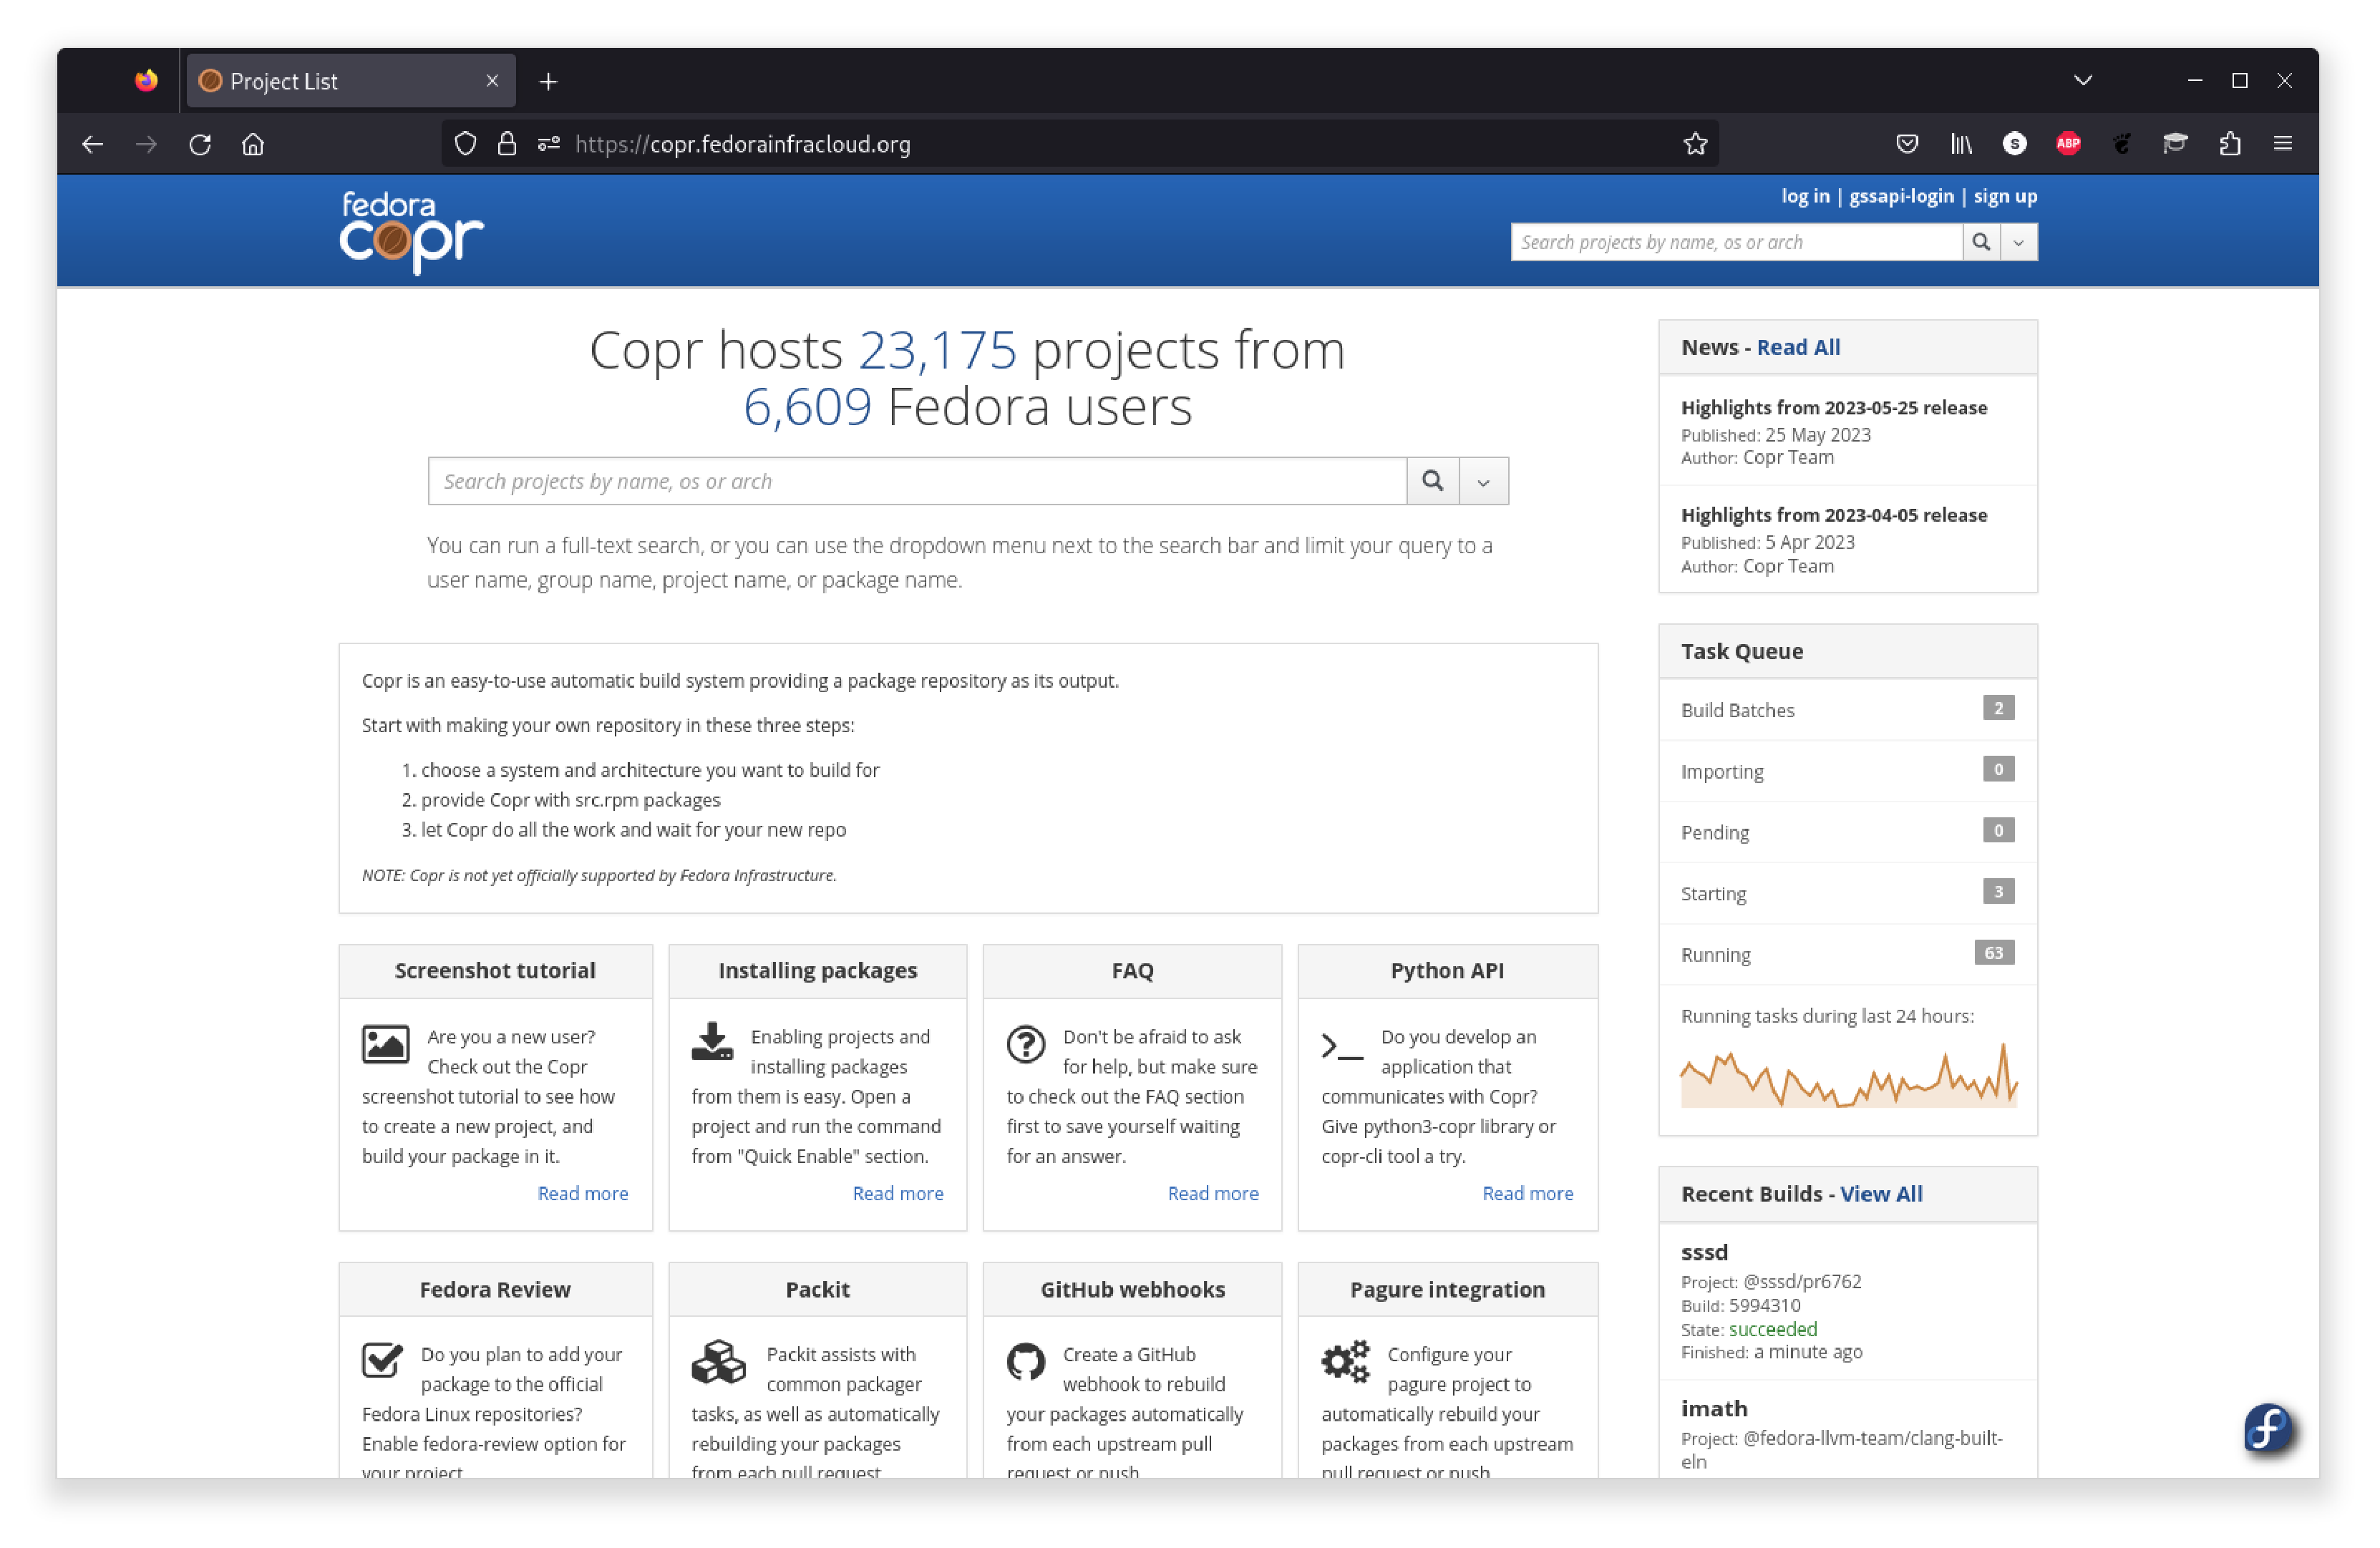
\includegraphics[width=1.0\textwidth,keepaspectratio=true,draft=\ddst]{img/rpms/copr.eps}
\end{center}
The Copr server is the closest thing to the official Fedora build system named \href{https://koji.fedoraproject.org/koji}{Koji}. \\
Also Copr has all the testing tools required to full-proof your RPM package before submitting it to Koji. \\[0.25cm]
The Copr user documentation is available at: \\[0.25cm]
\href{https://docs.pagure.org/copr.copr/user\_documentation.html}{https://docs.pagure.org/copr.copr/user\_documentation.html}
\newpage
\noindent Using Copr requires first of all to create a Fedora account at: \href{https://accounts.fedoraproject.org/}{https://accounts.fedoraproject.org/}
This Fedora account will be used for all Fedora resources, in particular Koji (see [Sec.~\ref{kojib}]). 
\begin{enumerate}
\item Register at \href{https://accounts.fedoraproject.org/}{https://accounts.fedoraproject.org/}
\begin{center}
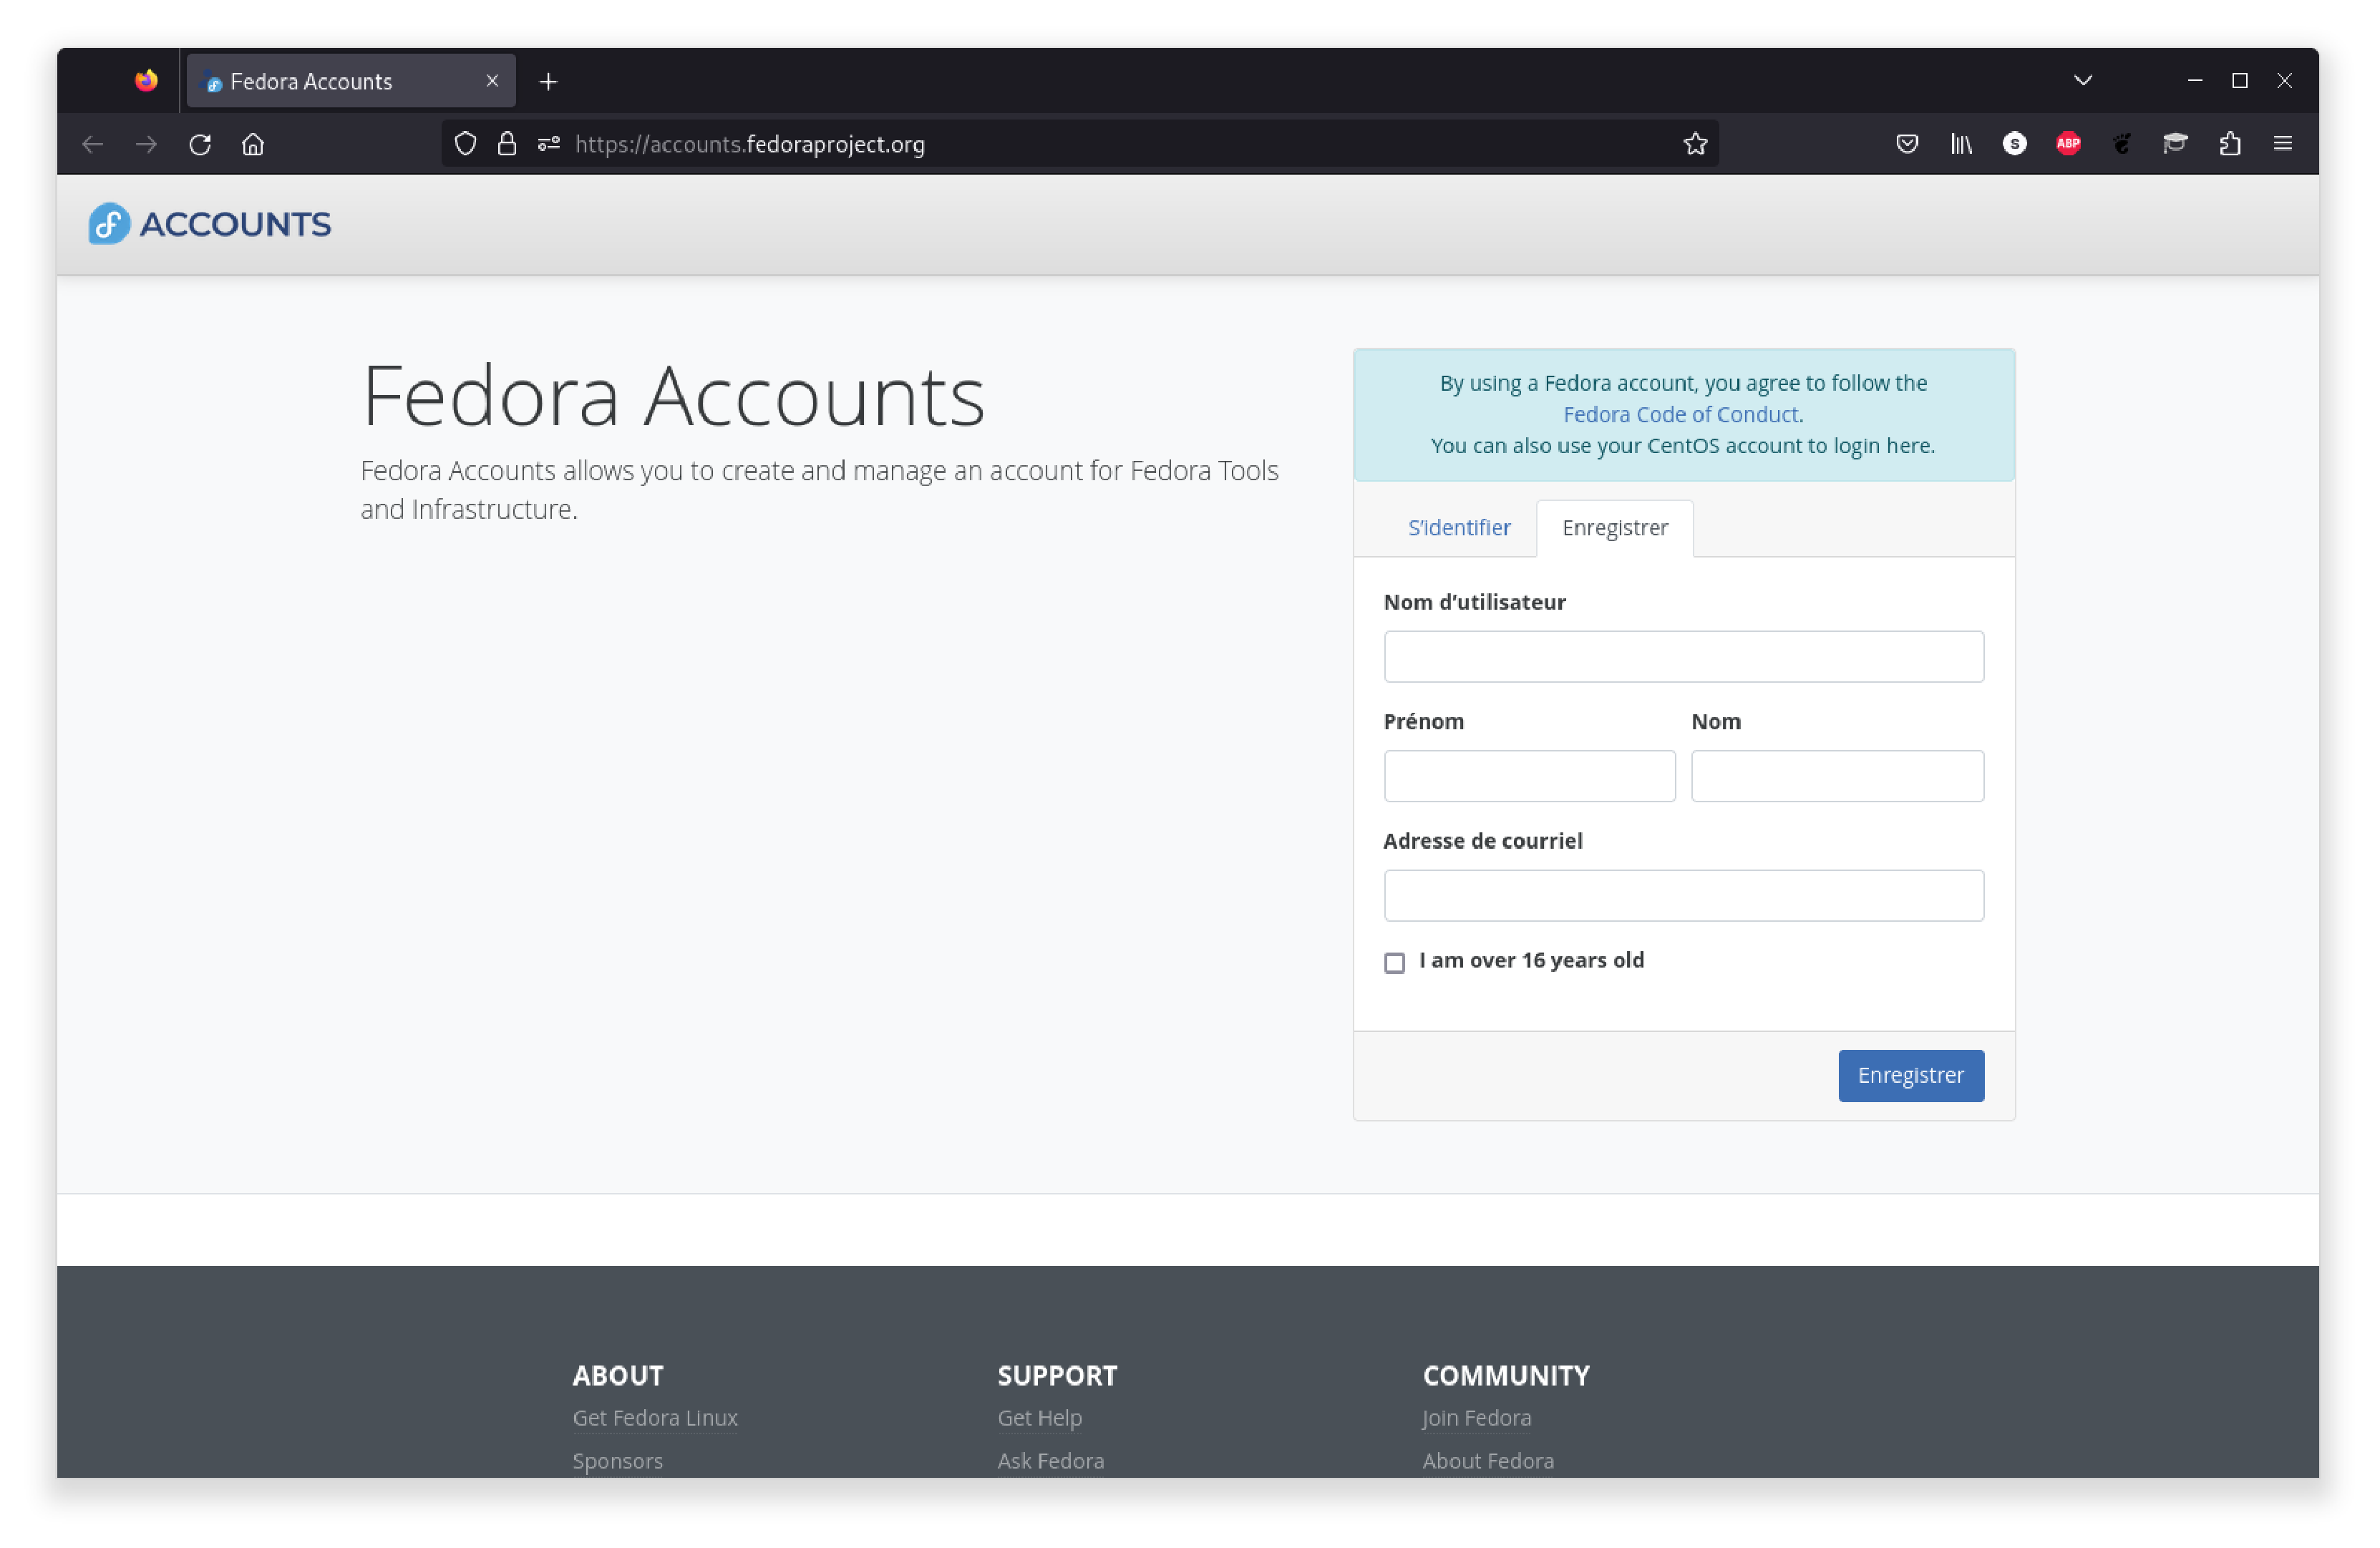
\includegraphics[width=0.7\textwidth,keepaspectratio=true,draft=\ddst]{img/rpms/f-account.eps}
\end{center}
\item After the registration sign the \href{https://docs.fedoraproject.org/en-US/legal/fpca/}{Fedora project Contributor Agreement}. 
\item Navigate to \href{https://copr.fedorainfracloud.org}{https://copr.fedorainfracloud.org} and login using your Fedora account. 
\begin{center}
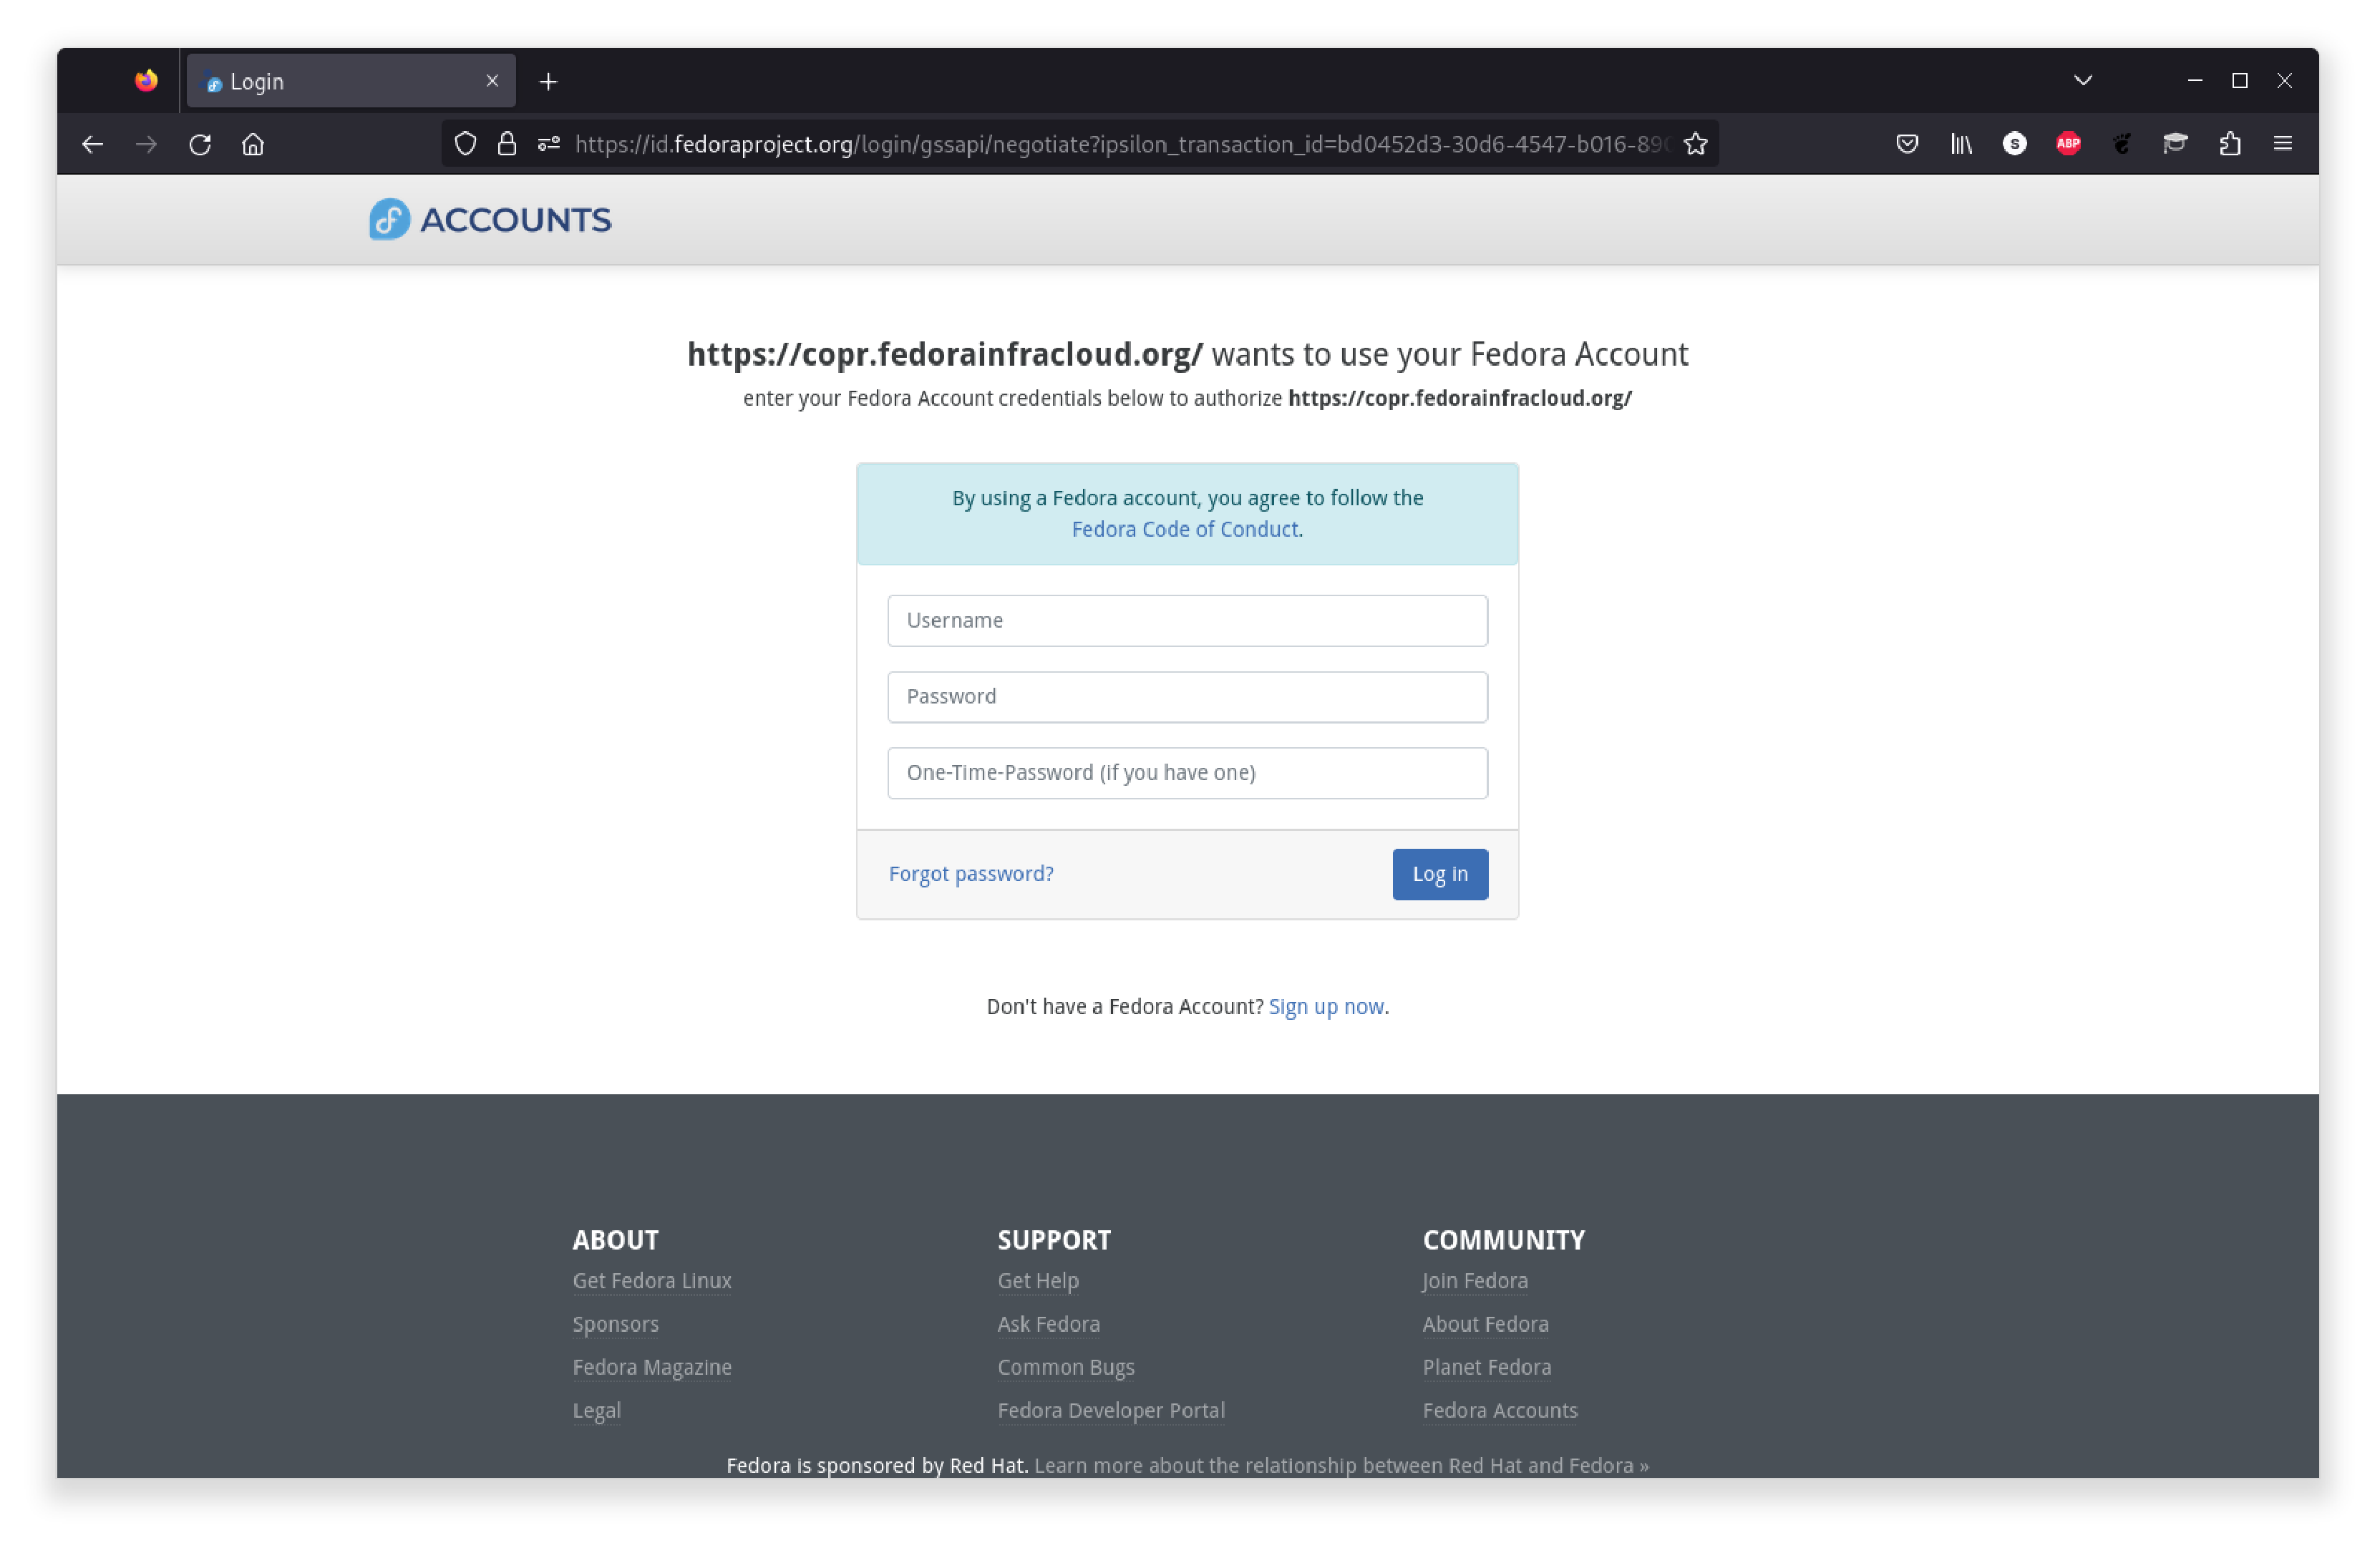
\includegraphics[width=0.7\textwidth,keepaspectratio=true,draft=\ddst]{img/rpms/c-login.eps}
\end{center}
Remember, and store, the Fedora username and password that you created at this stage since they will be used on regular basis if you integrate the Fedora network and building tools (Koji, see [Sec.~\ref{kojib}]). 
\newpage
\item Create a new project to host your work in Copr: 
\begin{itemize}
\item Describe the project (you can use Markdown):
\begin{center}
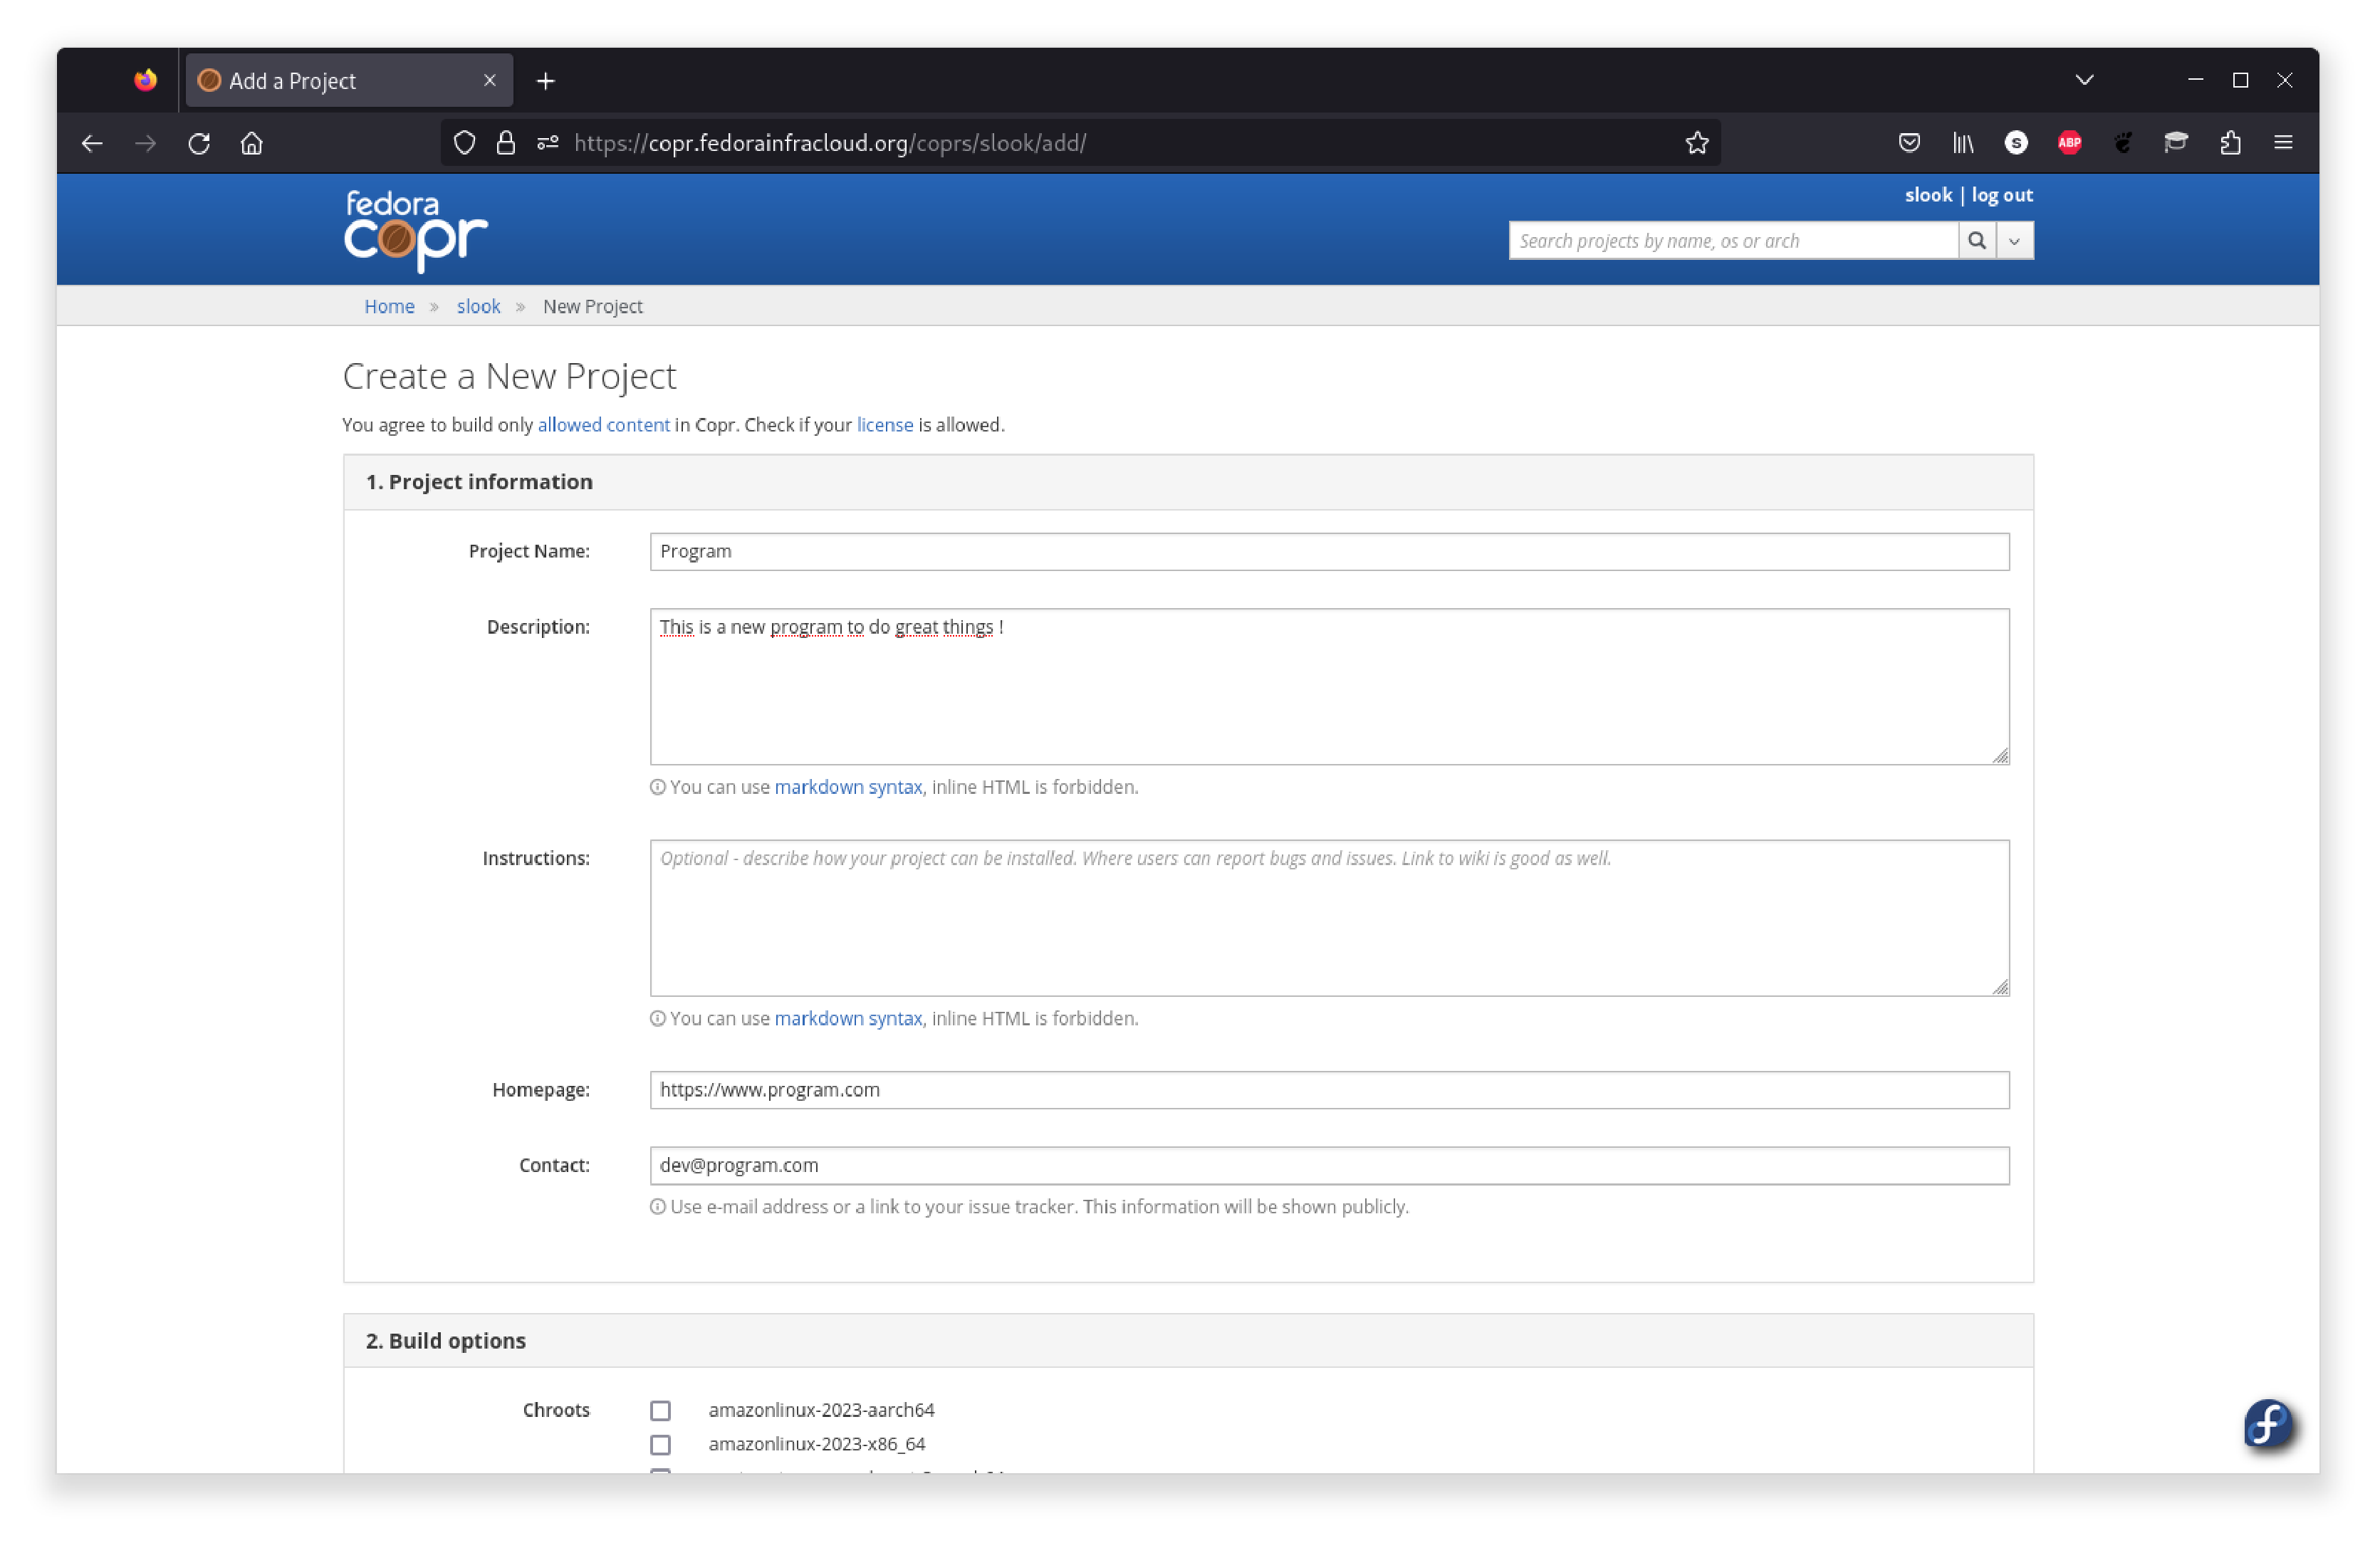
\includegraphics[width=0.6\textwidth,keepaspectratio=true,draft=\ddst]{img/rpms/new-p-1.eps}
\end{center}
\item Select the target architecture(s):
\begin{center}
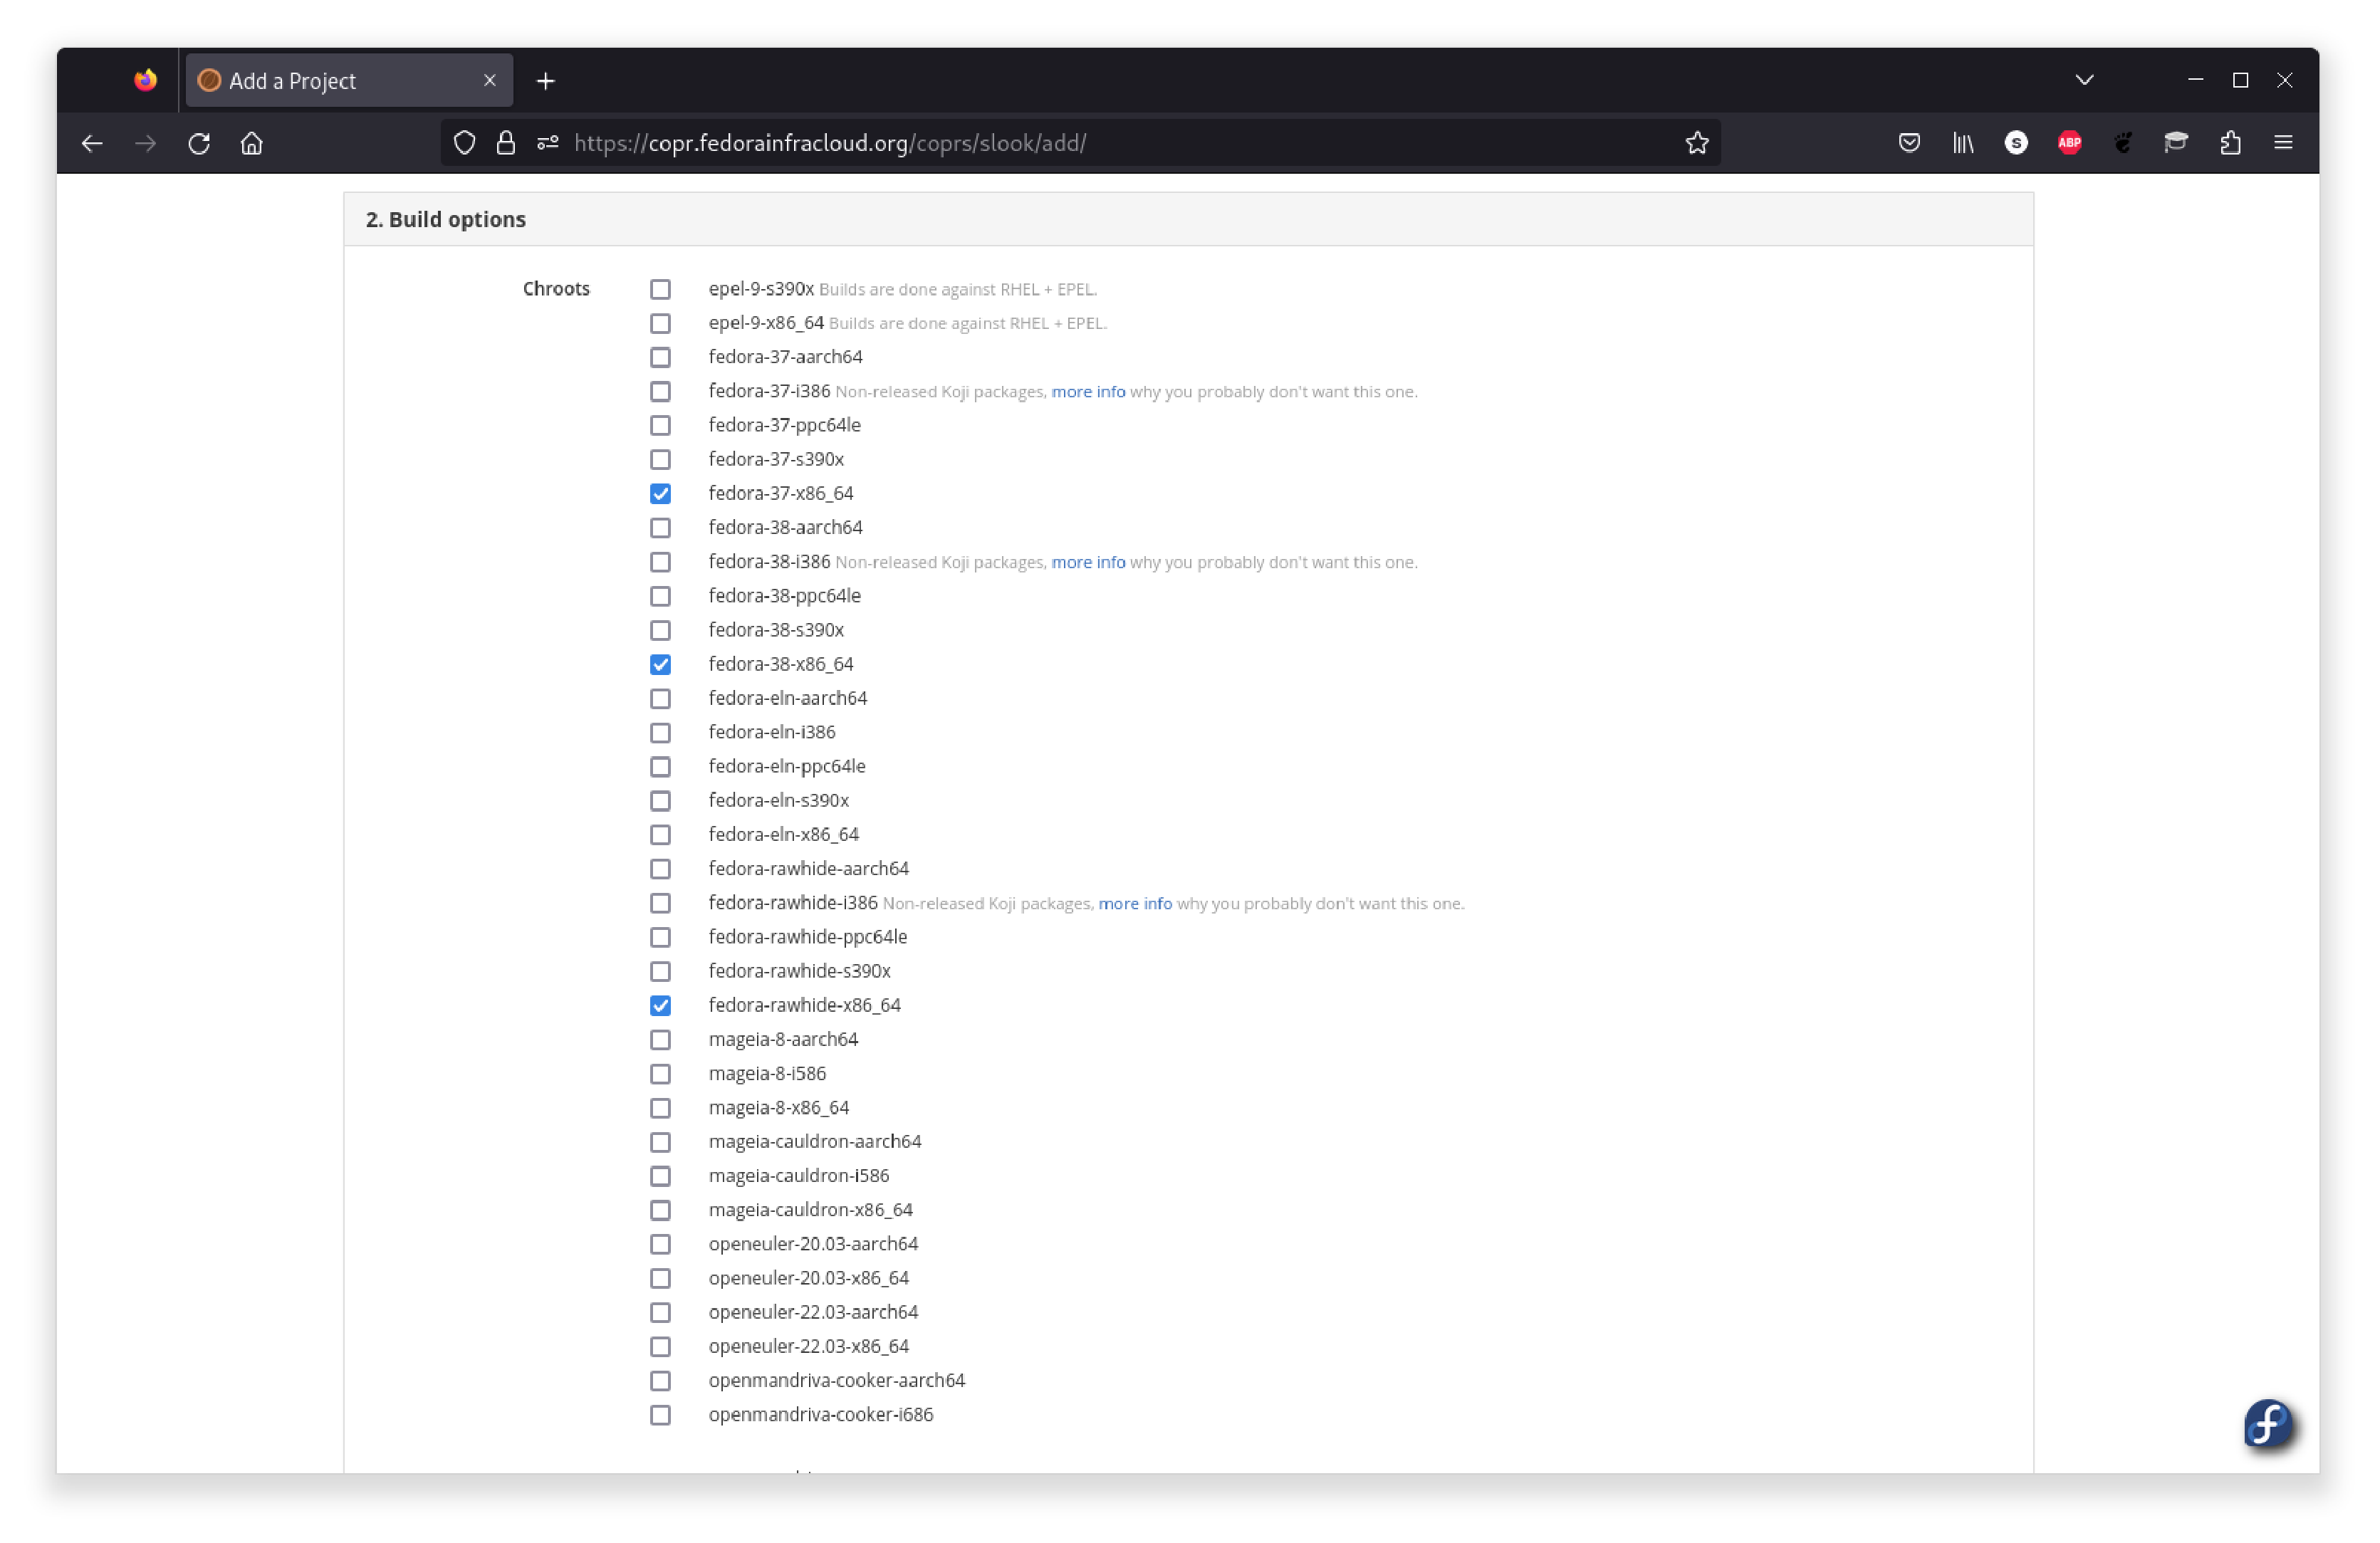
\includegraphics[width=0.6\textwidth,keepaspectratio=true,draft=\ddst]{img/rpms/new-p-2.eps}
\end{center}
\item Scroll down and click on "Create":
\begin{center}
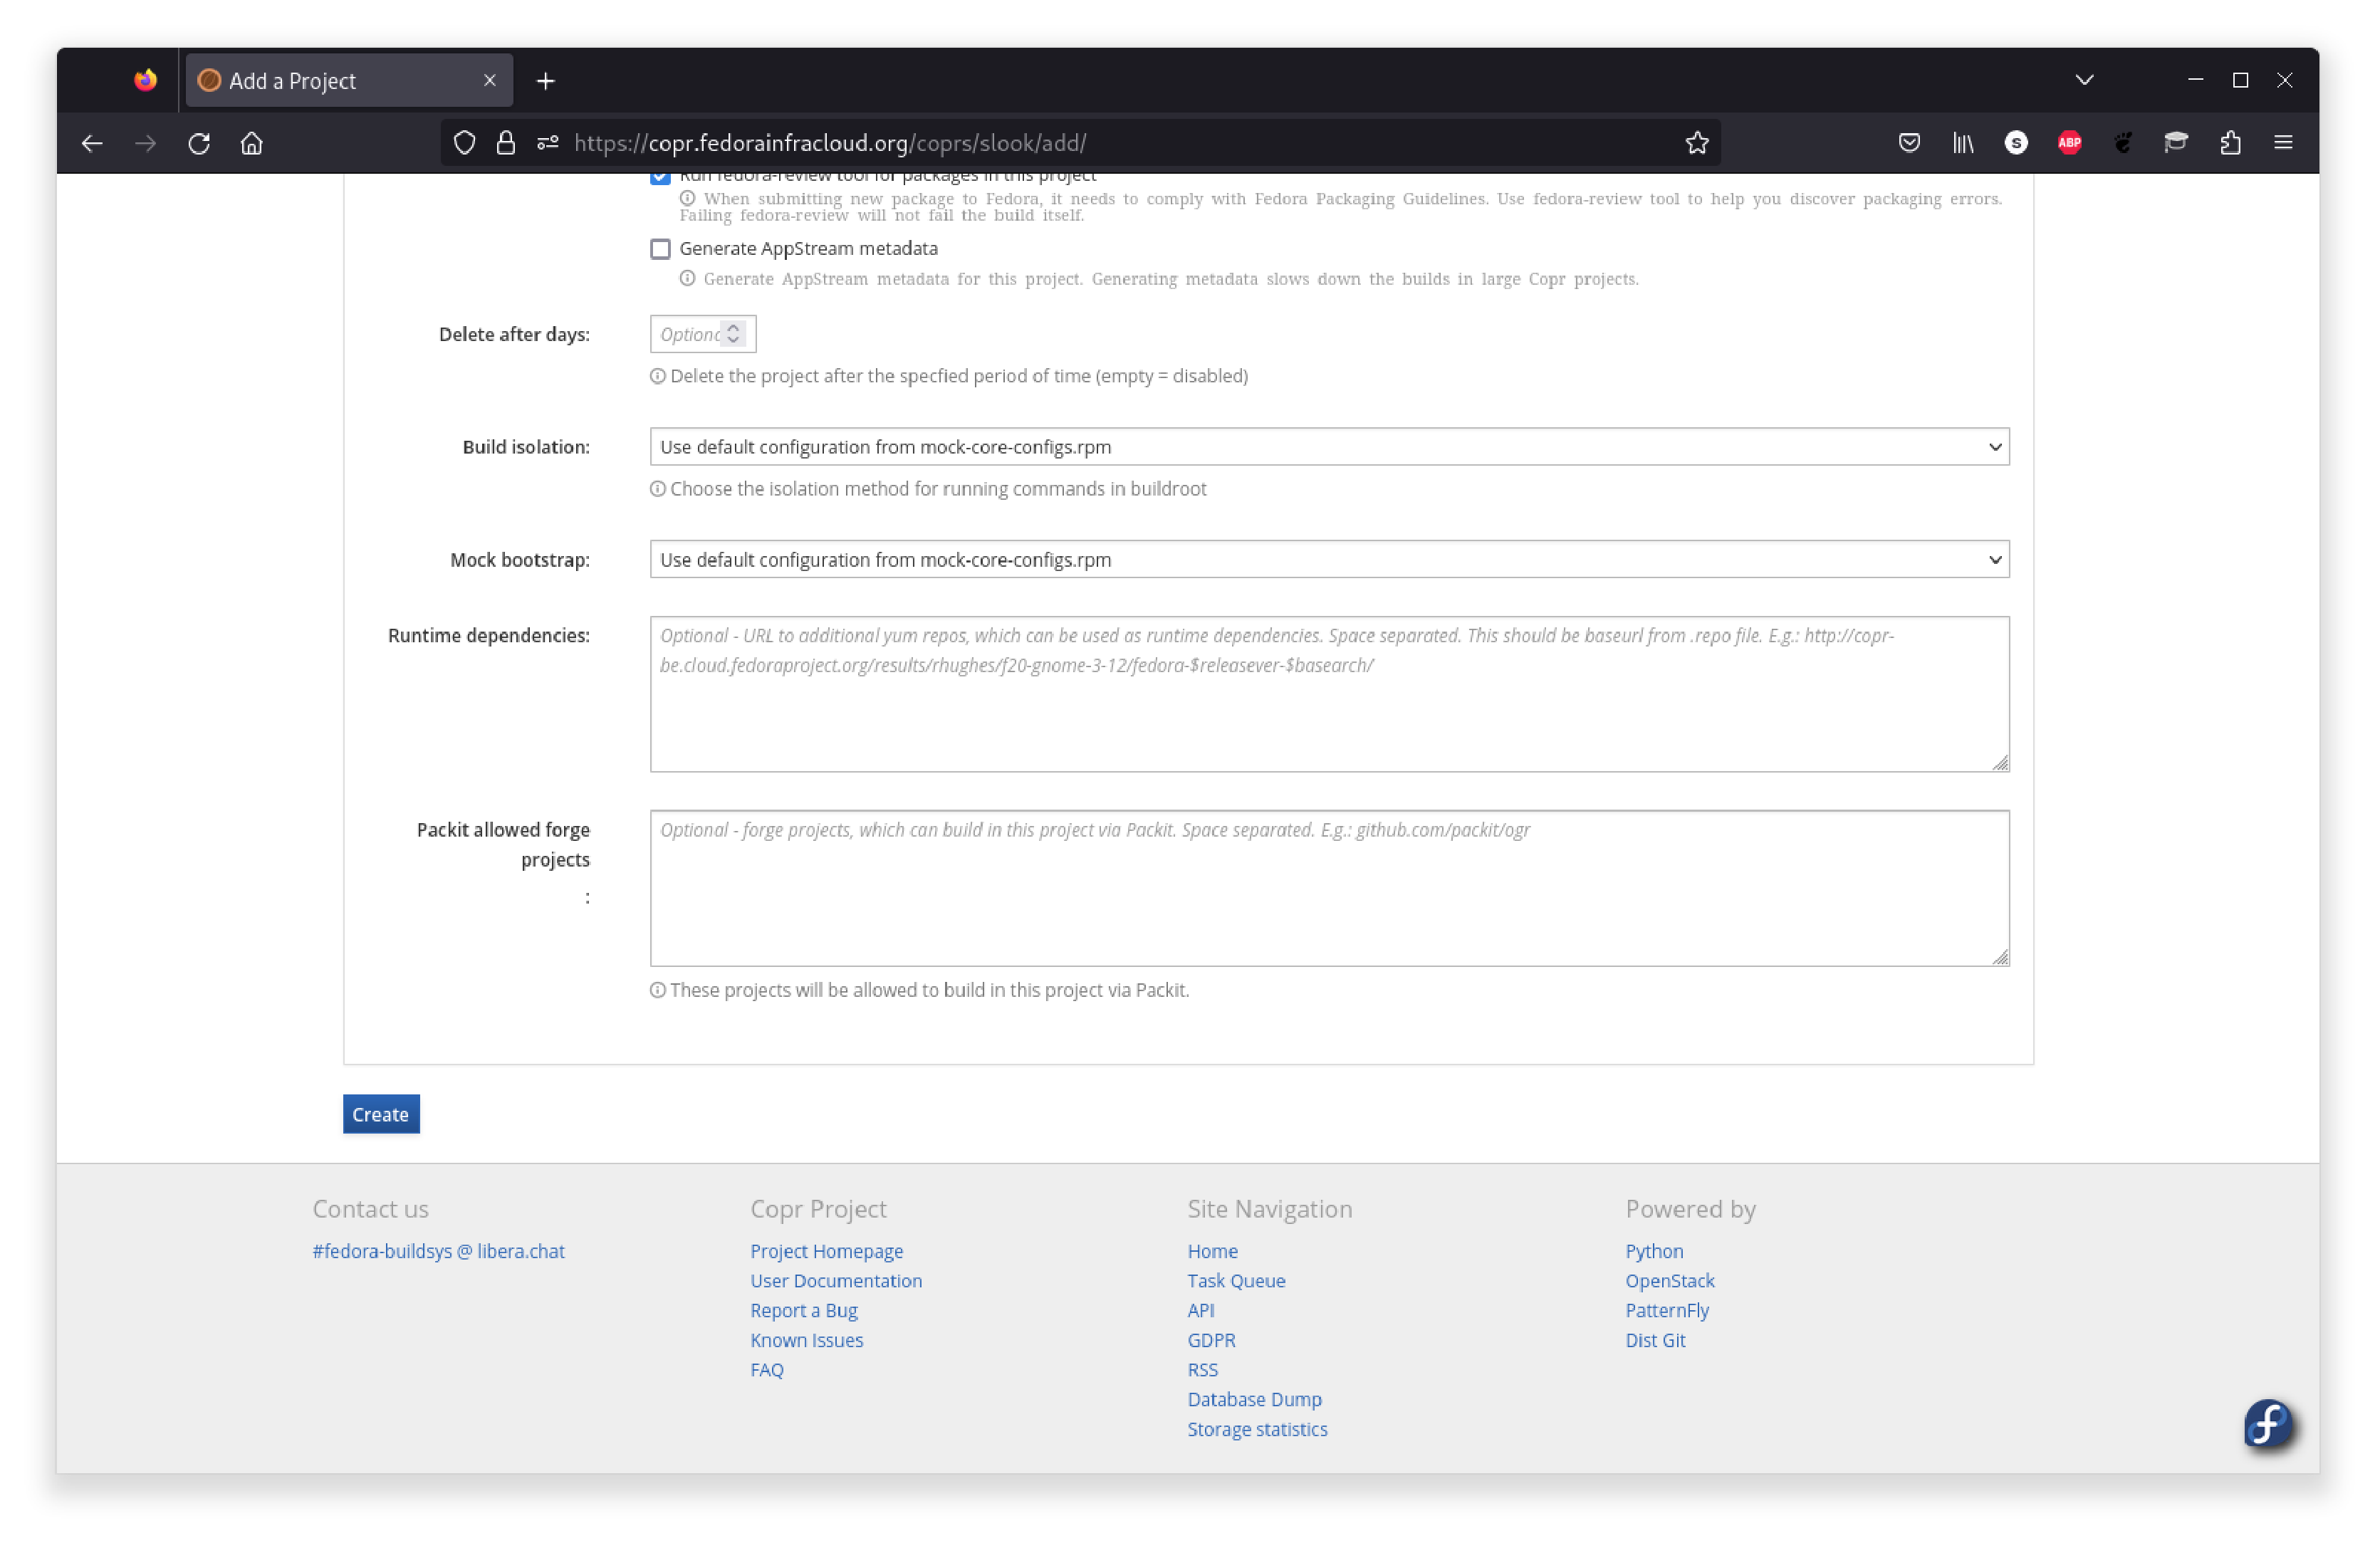
\includegraphics[width=0.6\textwidth,keepaspectratio=true,draft=\ddst]{img/rpms/new-p-3.eps}
\end{center}
\end{itemize}
\newpage
\item Then "Submit a New Build" for the project:
\begin{center}
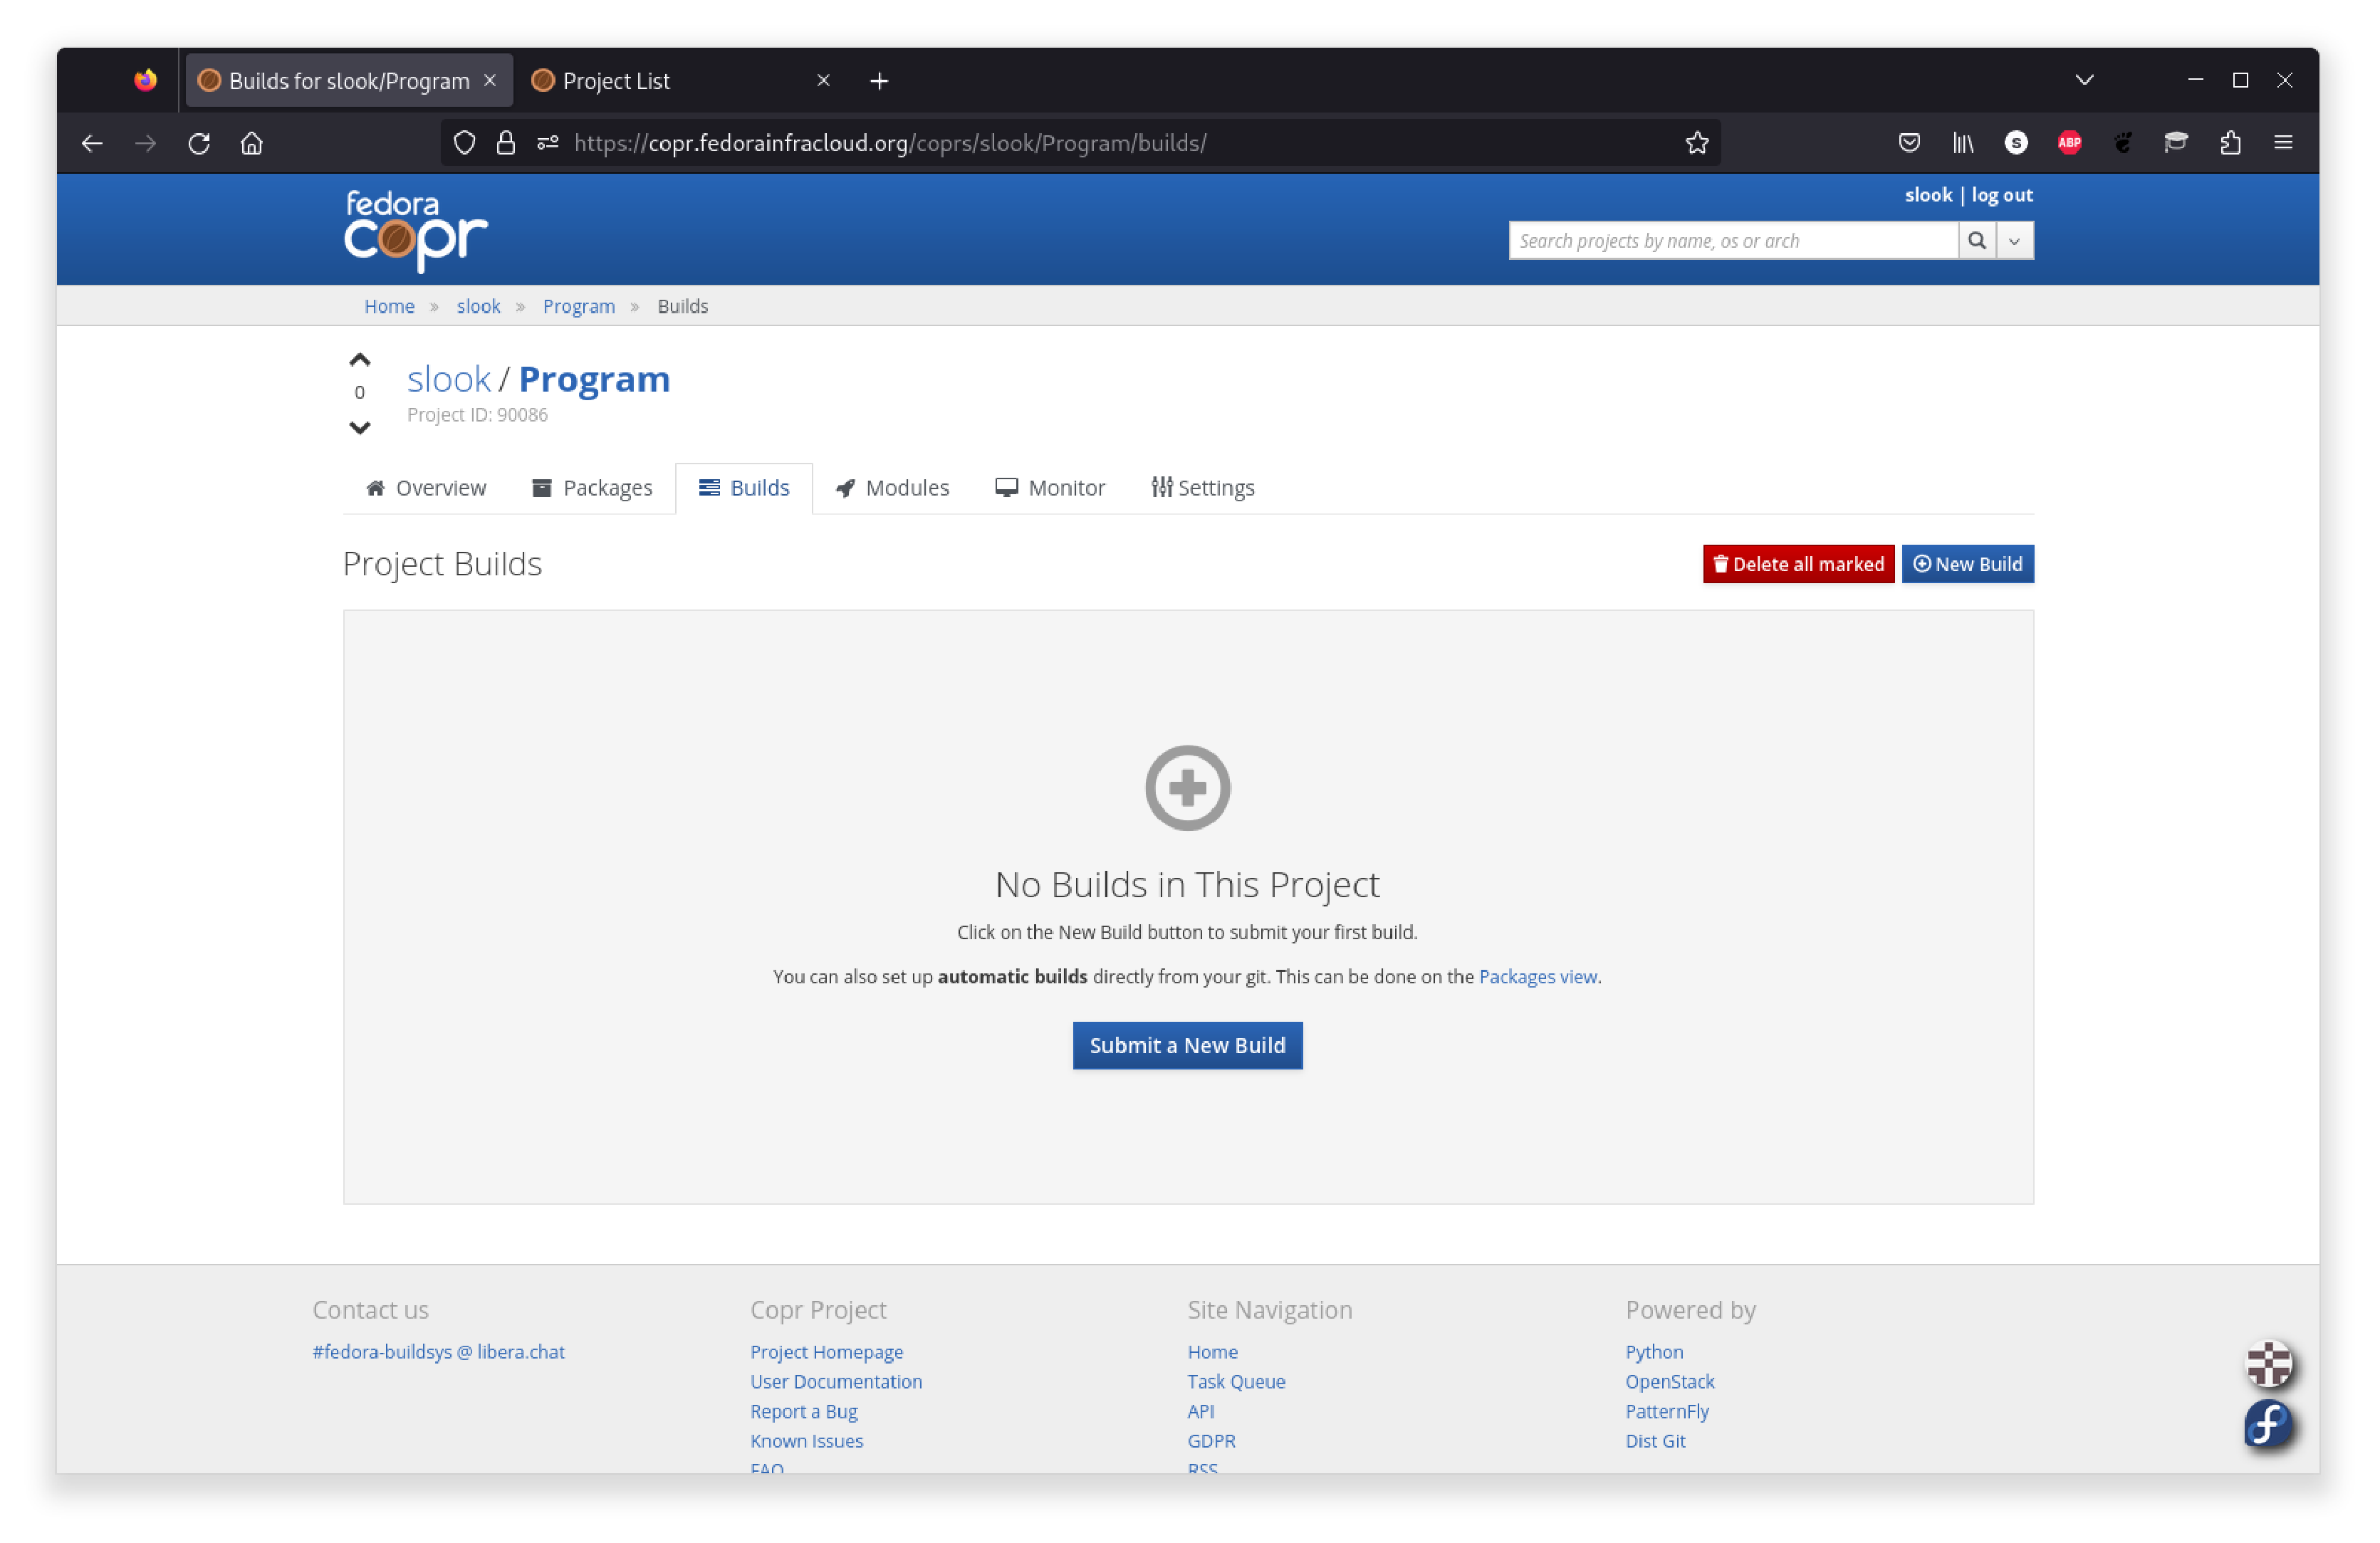
\includegraphics[width=0.6\textwidth,keepaspectratio=true,draft=\ddst]{img/rpms/build-1.eps}
\end{center}
\item Build the project:
\begin{itemize}
\item Build from URL, and specify the URL of your "\bftt{.spec}" file:
\begin{center}
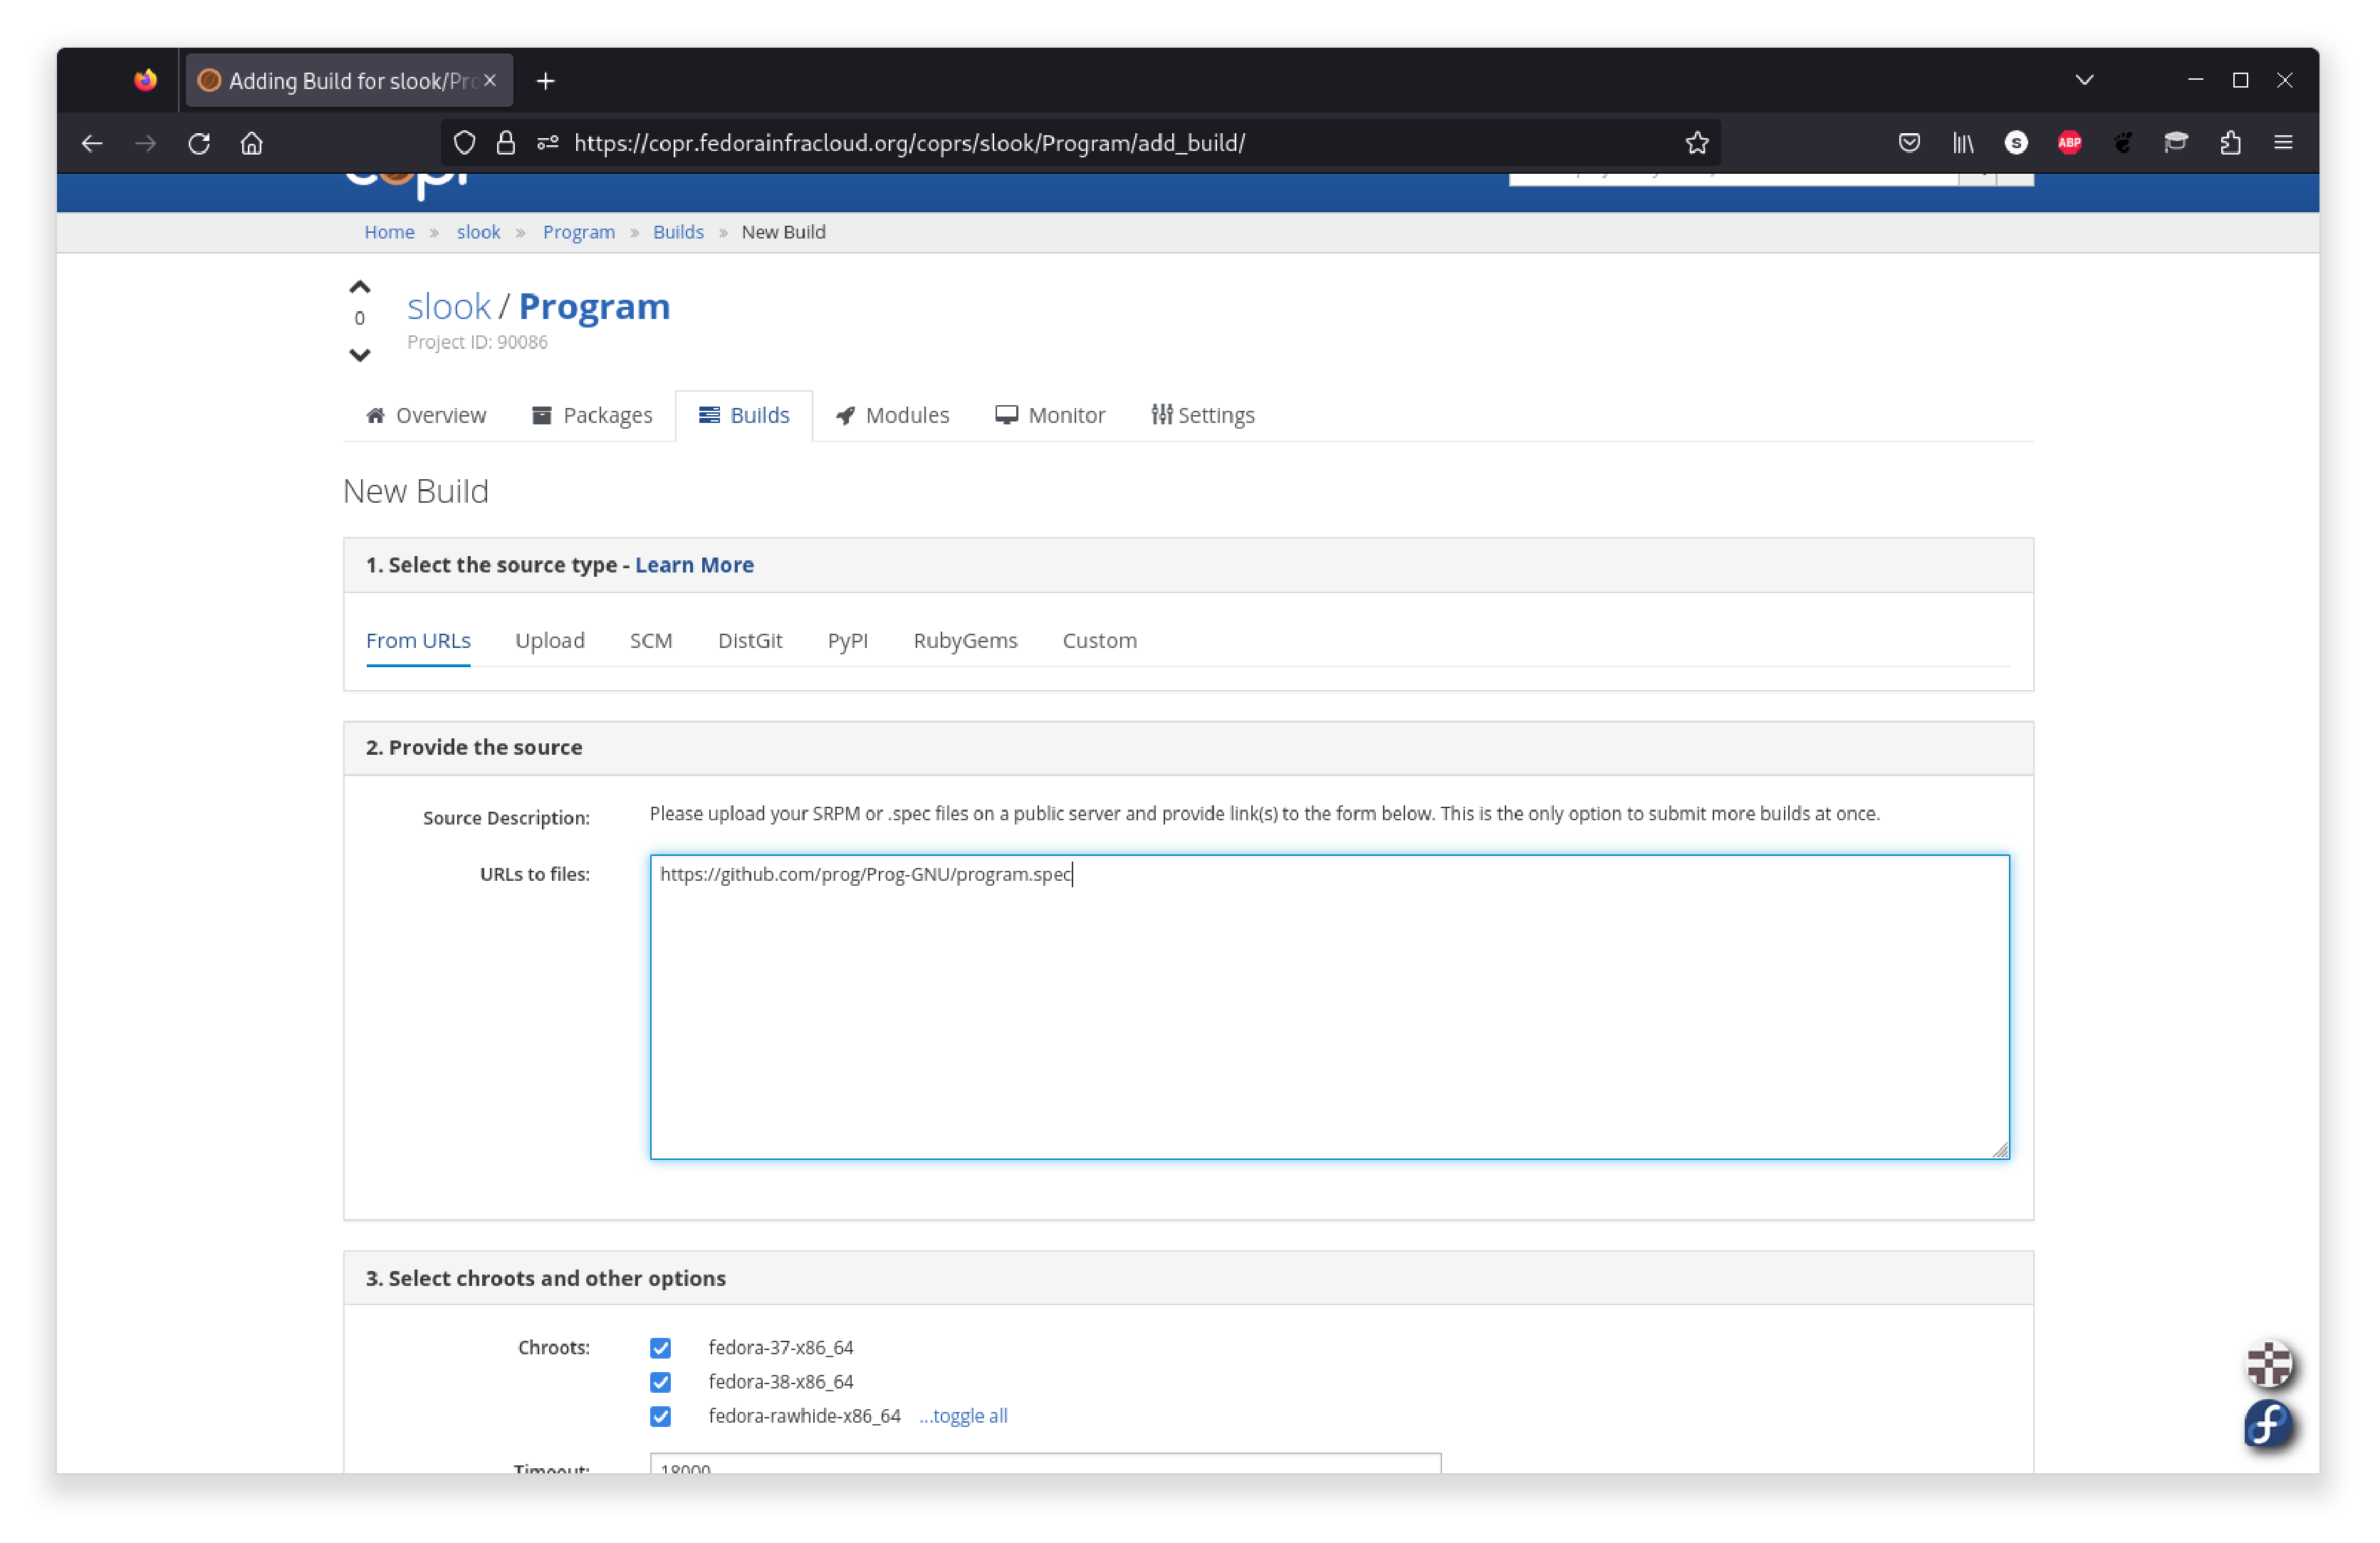
\includegraphics[width=0.6\textwidth,keepaspectratio=true,draft=\ddst]{img/rpms/build-2.eps}
\end{center}
\item Scroll down and simply click on "Build":
\begin{center}
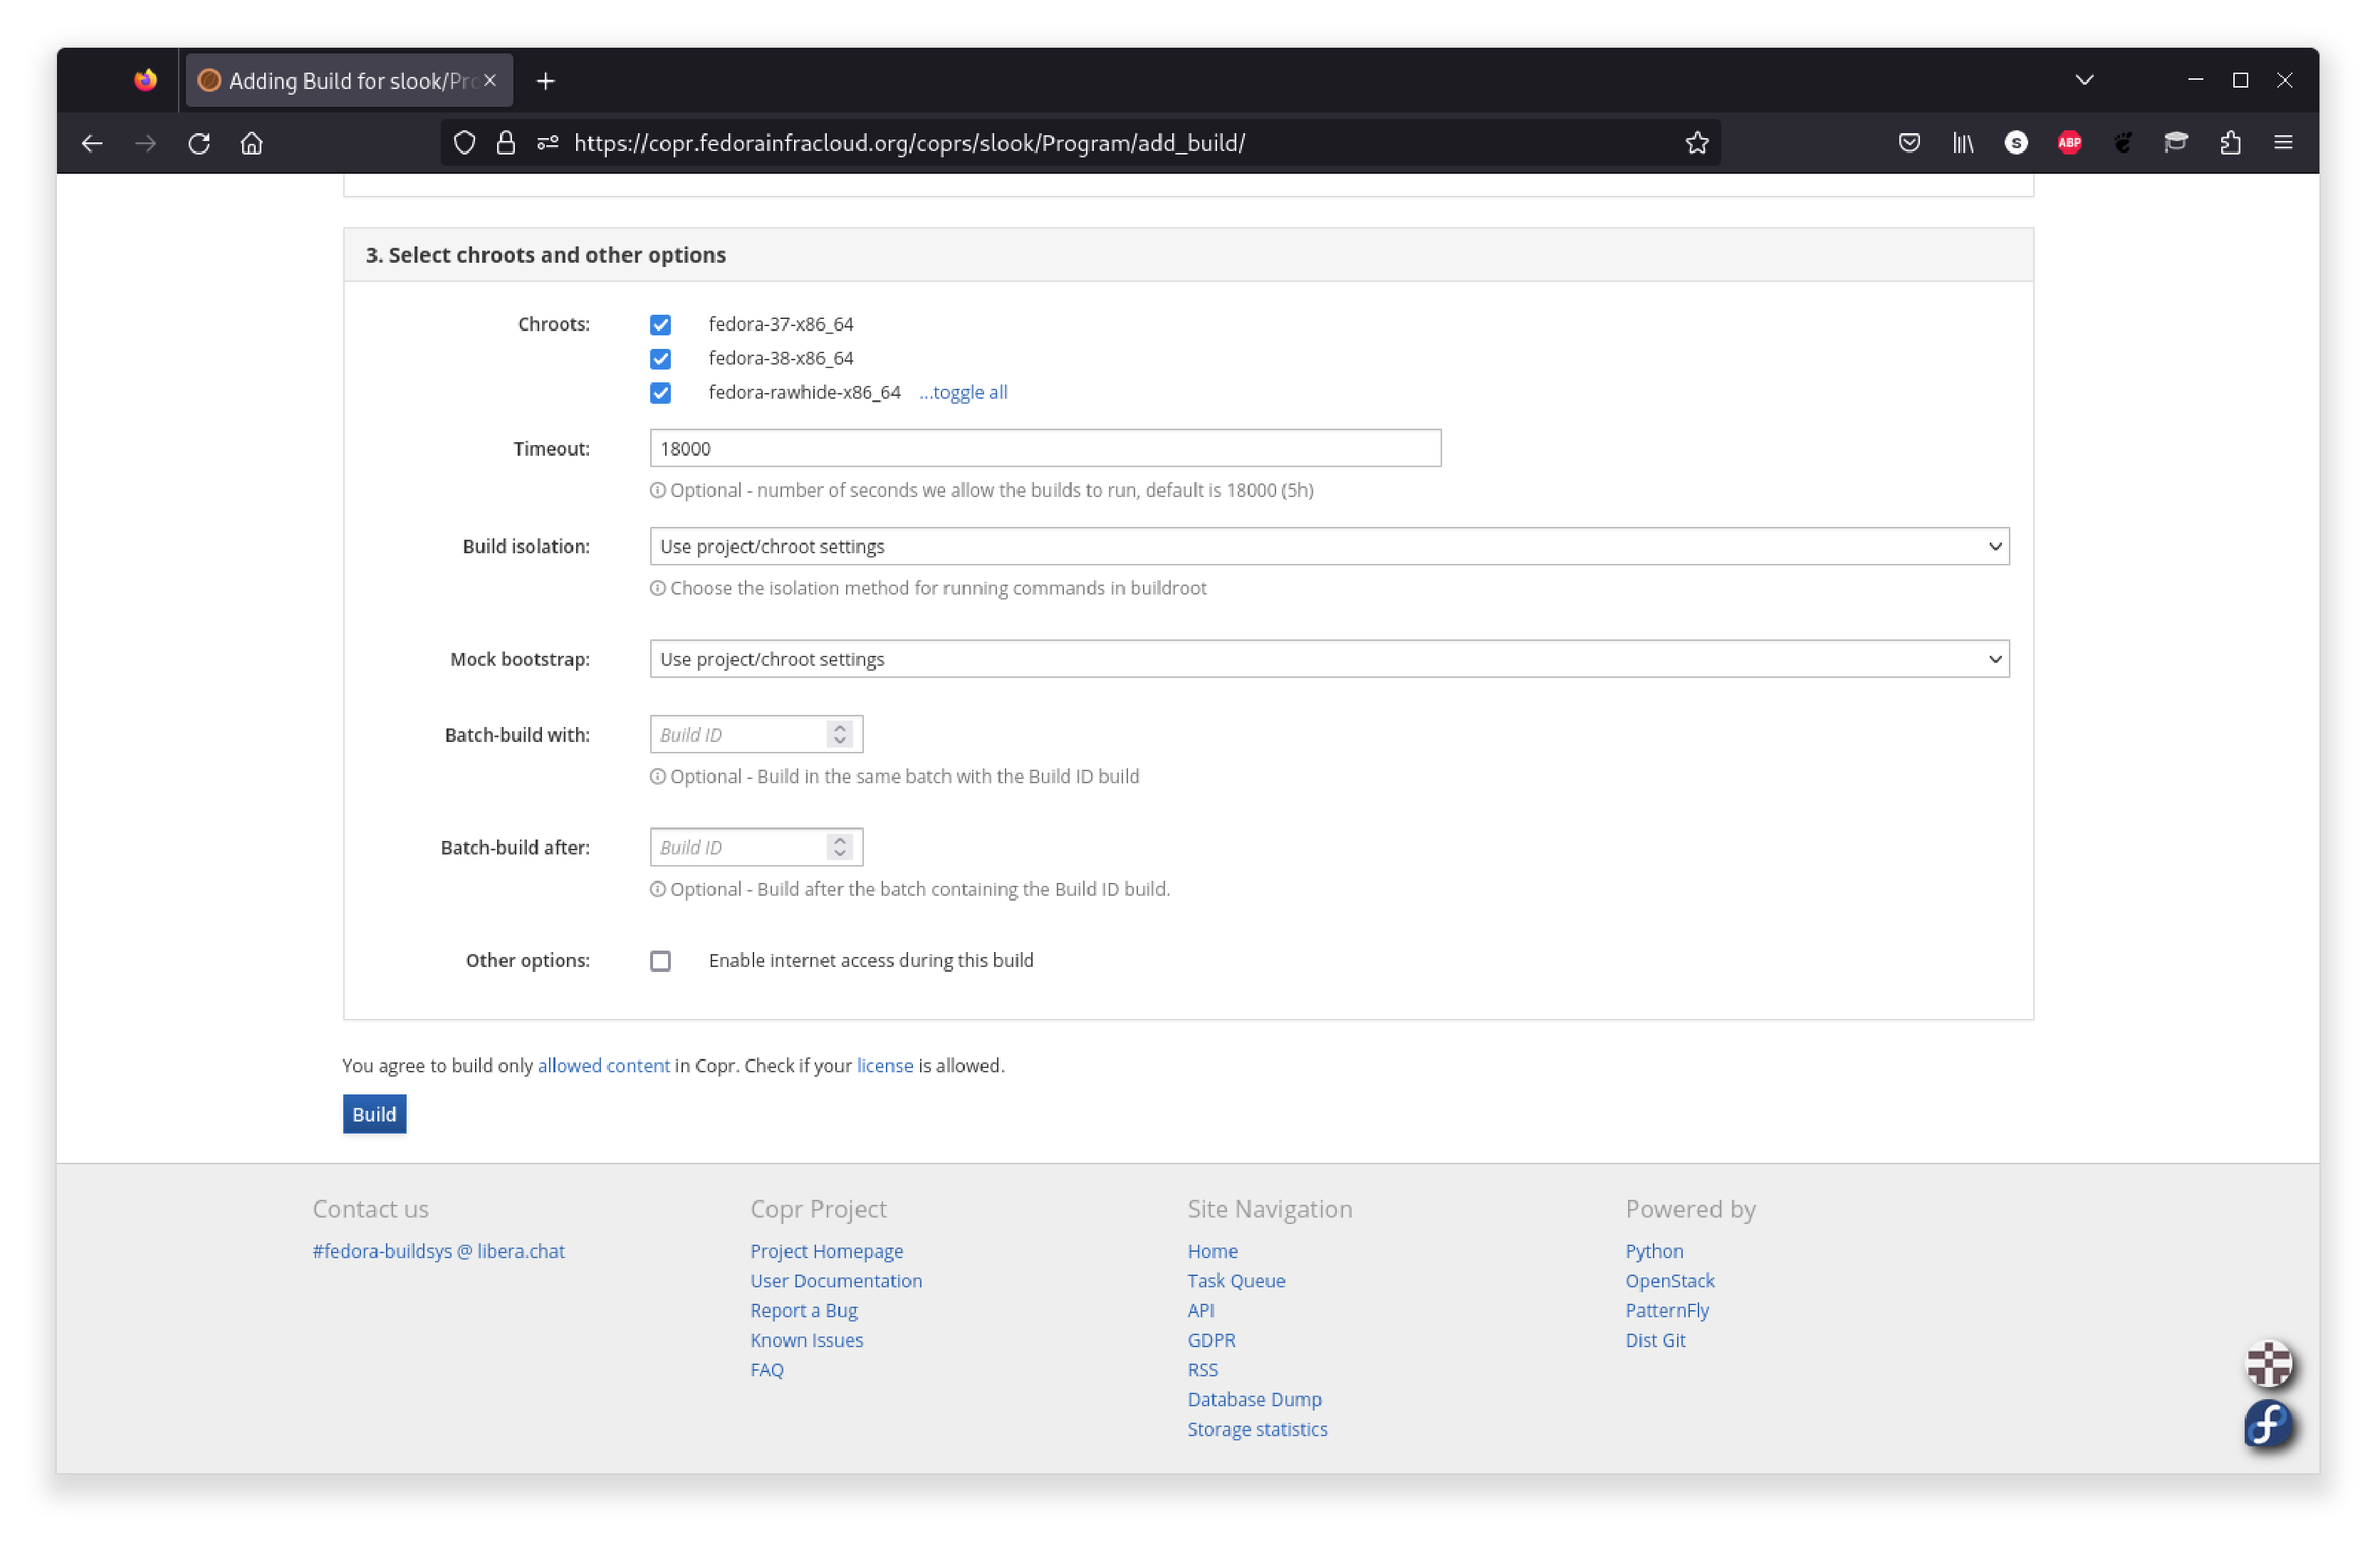
\includegraphics[width=0.6\textwidth,keepaspectratio=true,draft=\ddst]{img/rpms/build-3.eps}
\end{center}
\end{itemize}
\end{enumerate}
At this point Copr is going to use the specified "\bftt{.spec}" file to build the RPMs of your project. \\
Providing that the "\bftt{.spec}" file properly describes the sources location and the actions needed to build the RPM, 
then nothing else is required. 

\subsubsection{Koji build}
\label{kojib}

\href{https://fedoraproject.org/wiki/Koji}{Koji} is the official RPM build system of the Fedora project: \href{https://koji.fedoraproject.org/koji}{https://koji.fedoraproject.org/koji}
\begin{center}
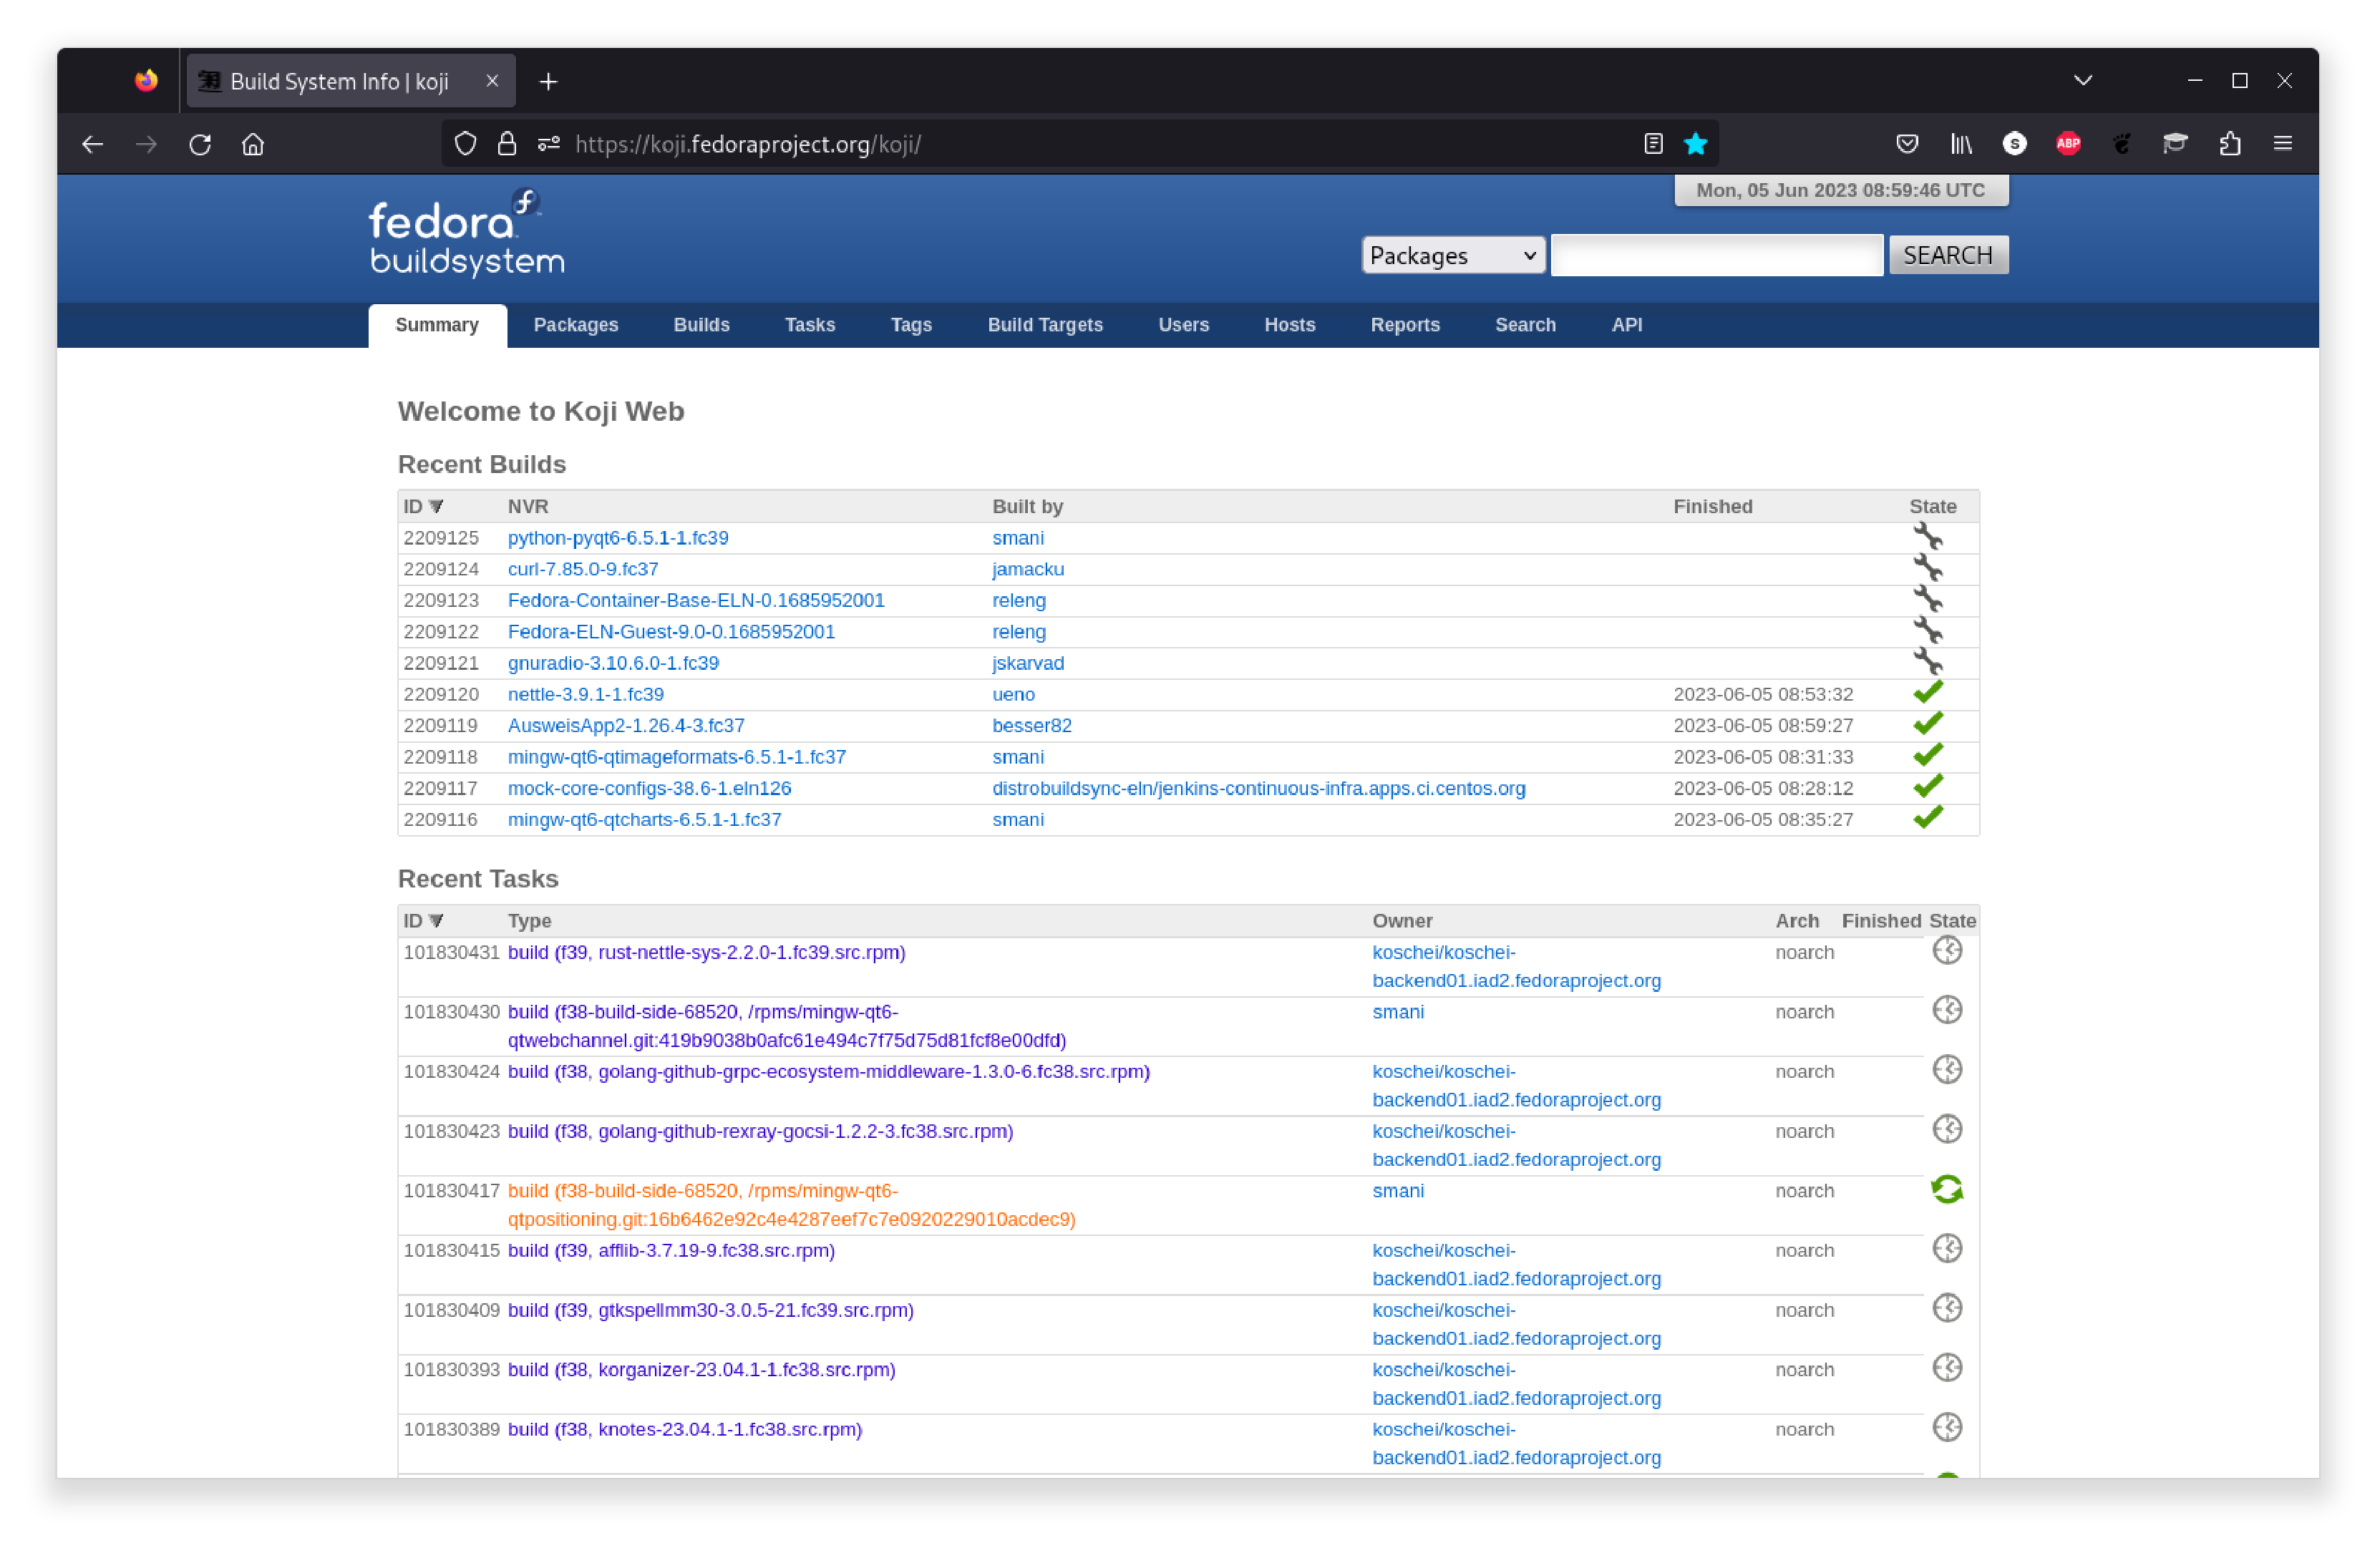
\includegraphics[width=1.0\textwidth,keepaspectratio=true,draft=\ddst]{img/rpms/koji.eps}
\end{center}
Even if your RPM is not distributed by the Fedora project, it possible, if not recommended, to test build your RPM in the Koji environment. \\
To access and use Koji requires to be registered with a Fedora account (see [Sec.~\ref{coprb}]). 
Also to use Koji requires to use the command line. \\[0.25cm]
First of all to start using Koji you need to request a temporary access to the servers by initiating a new Kerberos ticket using your Fedora username and password:
\begin{script}
\fprompt{~} fkinit -u username
Enter your password and OTP concatenated.
(Ignore that the prompt is for only the token)
Password for username@FEDORAPROJECT.ORG: 
\fprompt{~} 
\end{script}
\\[-0.5cm]
\noindent This step is mandatory to allow you to request remote builds on the Koji servers.
\newpage
\noindent To build your RPM using Koji, create the source RPM (if not done already):
\begin{script}
\fprompt{~} \bftt{rpmbuild} \rtt{-bs} program.spec
\end{script}
\\[-0.75cm]
\noindent Then build the RPMs using:
\begin{script}
\fprompt{~} \bftt{koji} \rtt{build} \blue{--sractch rawhide} program-***.fc36.src.rpm
\end{script}
\\[-0.5cm]
\noindent Replace "\texttt{program-***.fc36.src.rpm}" by the name of your SRPM, then press \Enter. 
\begin{script}
\fprompt{~} \bftt{koji} \rtt{build} \blue{--sractch rawhide} program-***.fc36.src.rpm
Uploading srpm:  program-***.src.rpm
[=================================] 100\% 00:00:01   3.14 MiB   2.54 MiB/sec
Created task: 101830239
Task info: \href{https://koji.fedoraproject.org/koji/taskinfo?taskID=101830239}{https://koji.fedoraproject.org/koji/taskinfo?taskID=101830239}
Watching tasks (this may be safely interrupted)...
101830239 build (rawhide, program-***.fc36.src.rpm): free
\end{script}
\\[-0.25cm]
\noindent The link provided in the output of the commands provides you with a webpage to follow the build process:
\begin{center}
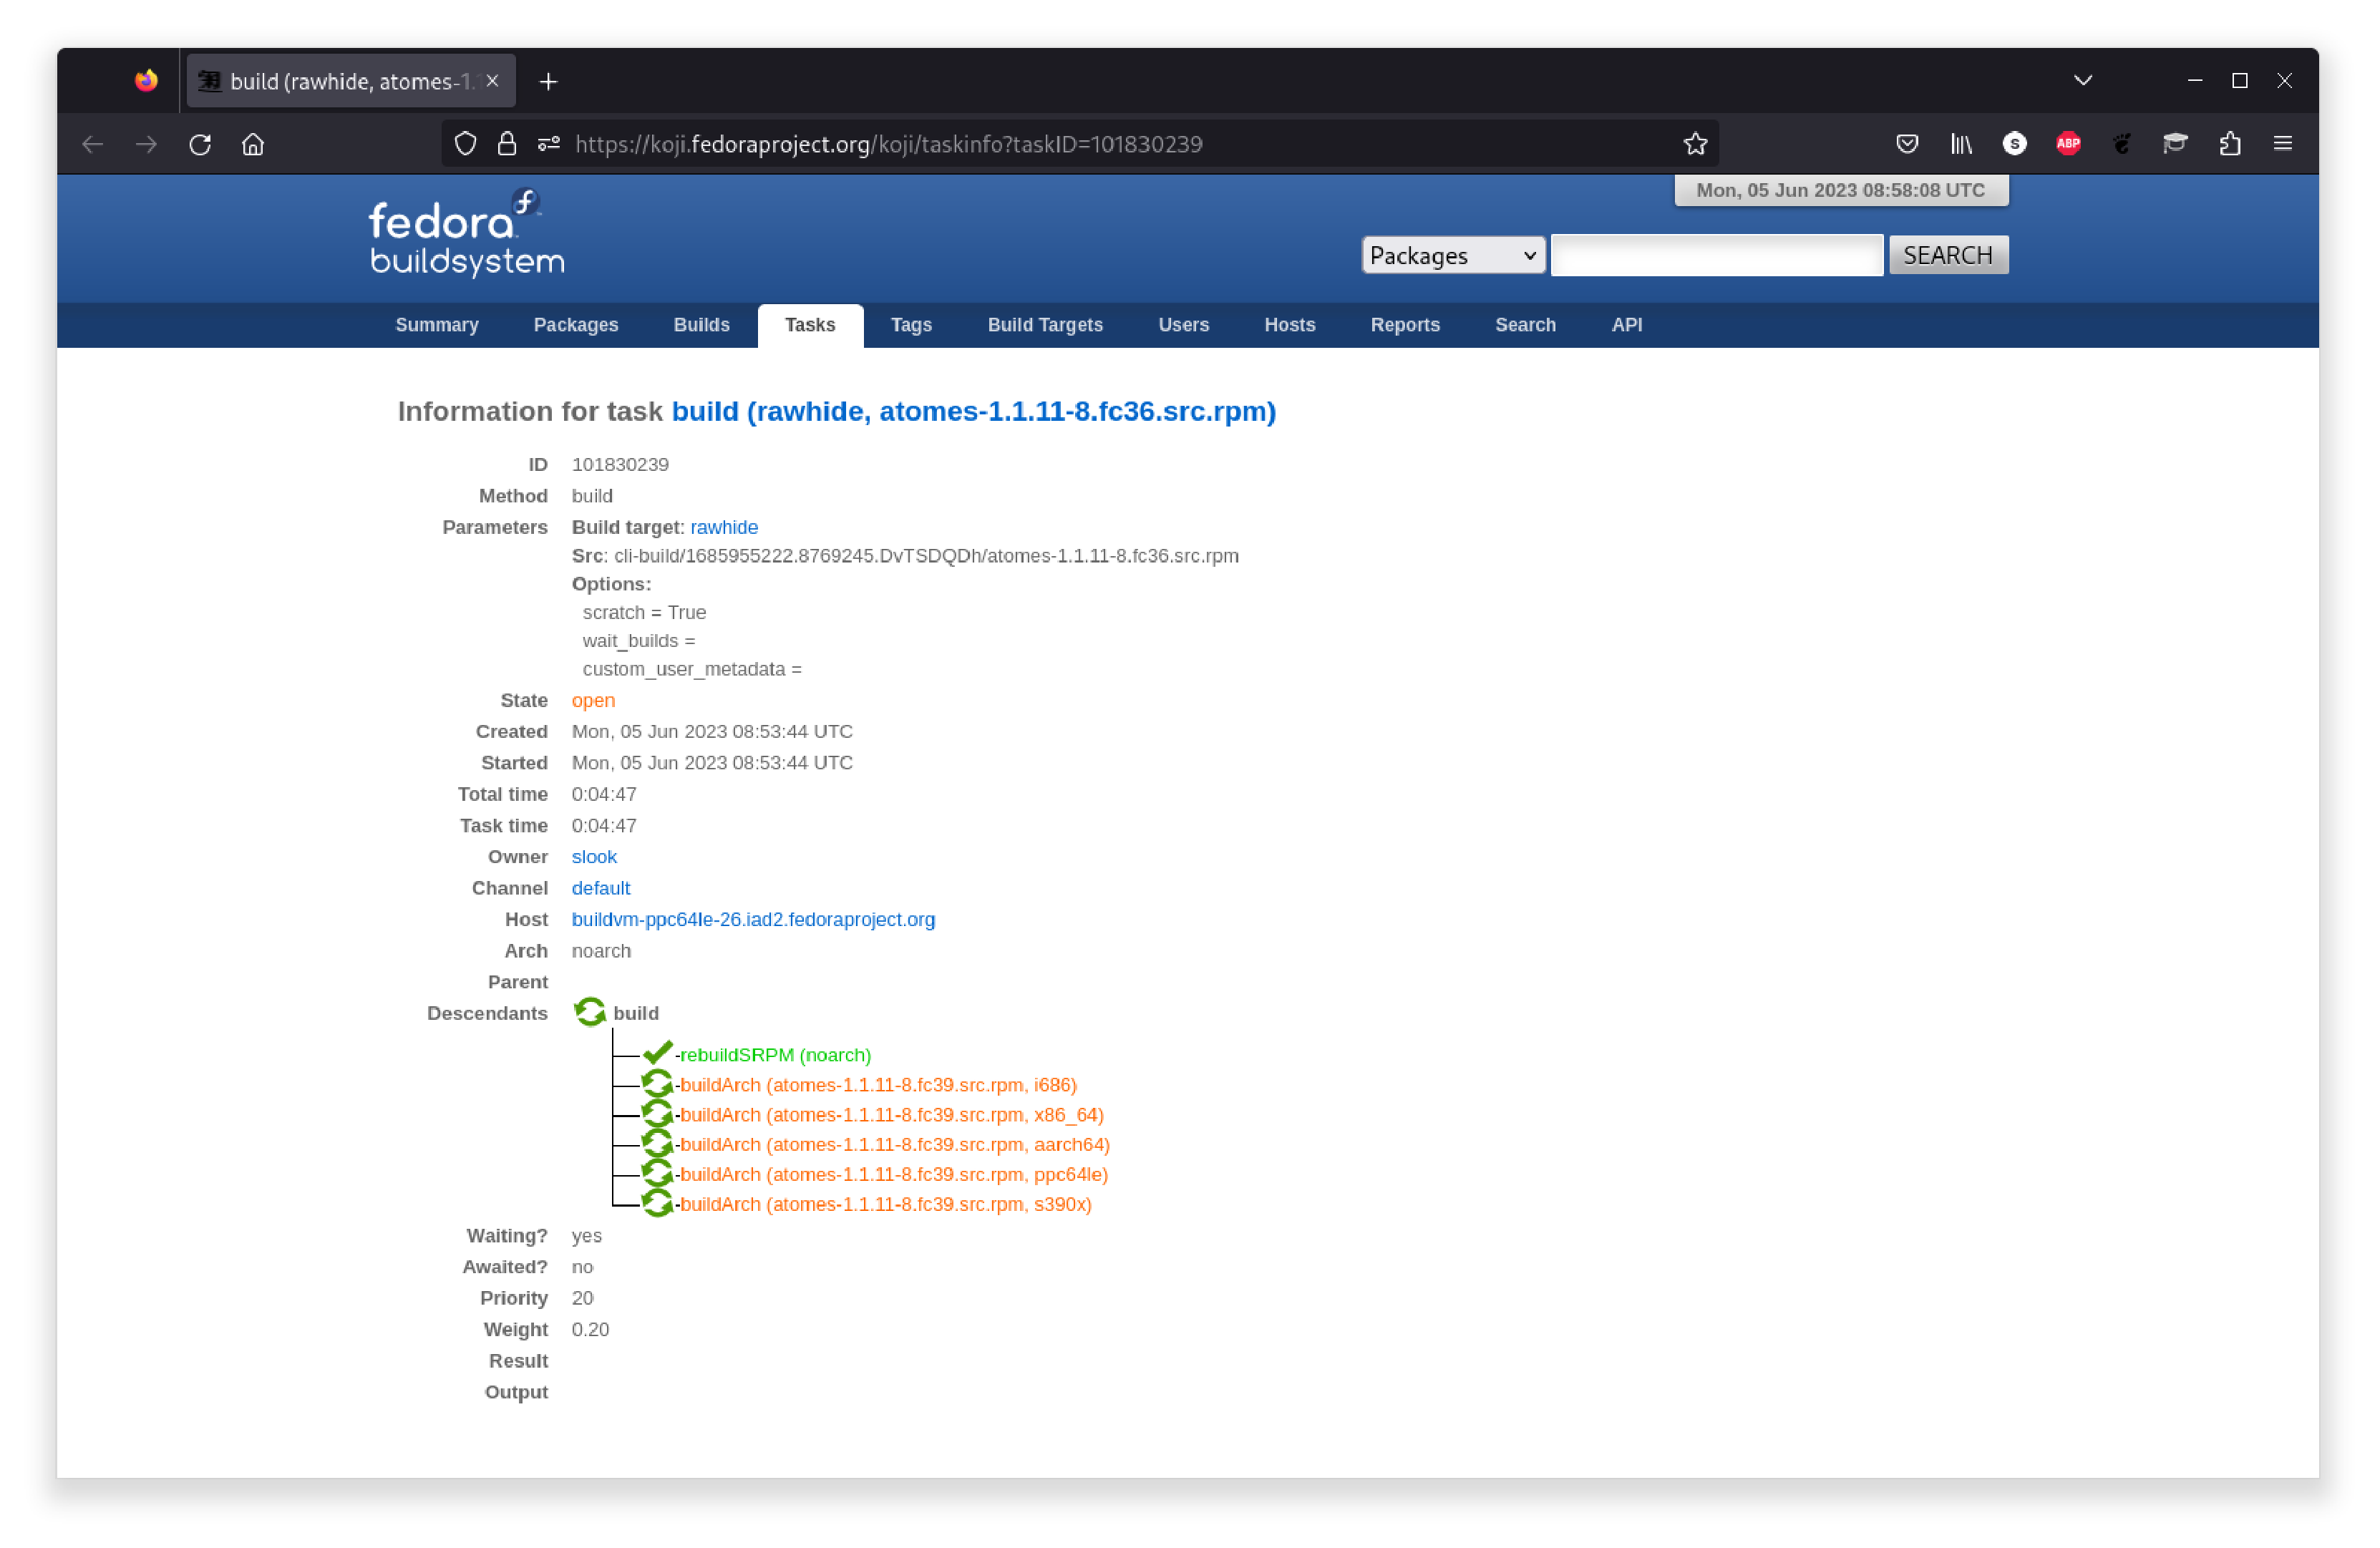
\includegraphics[width=1.0\textwidth,keepaspectratio=true,draft=\ddst]{img/rpms/koji-build.eps}
\end{center}
\newpage
\noindent The information is also provided and refreshed in the terminal:
{\scriptsize{
\begin{script}
\fprompt{~} \bftt{koji} \rtt{build} \blue{--sractch rawhide} program-***.fc36.src.rpm
Uploading srpm:  program-***.src.rpm
[=================================] 100\% 00:00:01   3.14 MiB   2.54 MiB/sec
Created task: 101830239
Task info: \href{https://koji.fedoraproject.org/koji/taskinfo?taskID=101830239}{https://koji.fedoraproject.org/koji/taskinfo?taskID=101830239}
Watching tasks (this may be safely interrupted)...
101830239 build (rawhide, program-***.fc36.src.rpm): free
101830239 build (rawhide, program-***.fc36.src.rpm): free -> open (buildvm-ppc64le-26.iad2.fedoraproject.org)
  101830240 rebuildSRPM (noarch): open (buildvm-ppc64le-02.iad2.fedoraproject.org)
  101830240 rebuildSRPM (noarch): open (buildvm-ppc64le-02.iad2.fedoraproject.org) -> closed
  0 free  1 open  1 done  0 failed
  101830324 buildArch (program-***.src.rpm, i686): free
  101830325 buildArch (program-***.src.rpm, x86\_64): free
\end{script}
}}
\\
\noindent Up to the end of the task:
{\scriptsize{
\begin{script}
\fprompt{~} \bftt{koji} \rtt{build} \blue{--sractch rawhide} program-***.fc36.src.rpm
Uploading srpm:  program-***.src.rpm
[=================================] 100\% 00:00:01   3.14 MiB   2.54 MiB/sec
Created task: 101830239
Task info: \href{https://koji.fedoraproject.org/koji/taskinfo?taskID=101830239}{https://koji.fedoraproject.org/koji/taskinfo?taskID=101830239}
Watching tasks (this may be safely interrupted)...
101830239 build (rawhide, program-***.fc36.src.rpm): free
101830239 build (rawhide, program-***.fc36.src.rpm): free -> open (buildvm-ppc64le-26.iad2.fedoraproject.org)
  101830240 rebuildSRPM (noarch): open (buildvm-ppc64le-02.iad2.fedoraproject.org)
  101830240 rebuildSRPM (noarch): open (buildvm-ppc64le-02.iad2.fedoraproject.org) -> closed
  0 free  1 open  1 done  0 failed
  101830324 buildArch (program-***.src.rpm, i686): free
  101830325 buildArch (program-***.src.rpm, x86\_64): free
  101830328 buildArch (program-***.src.rpm, s390x): free
  101830326 buildArch (program-***.src.rpm, aarch64): open (buildvm-a64-31.iad2.fedoraproject.org)
  101830327 buildArch (program-***.src.rpm, ppc64le): free
  101830324 buildArch (program-***.src.rpm, i686): free -> open (buildvm-x86-19.iad2.fedoraproject.org)
  101830328 buildArch (program-***.src.rpm, s390x): free -> open (buildvm-s390x-21.s390.fedoraproject.org)
  101830325 buildArch (program-***.src.rpm, x86\_64): free -> open (buildvm-x86-12.iad2.fedoraproject.org)
  101830327 buildArch (program-***.src.rpm, ppc64le): free -> open (buildvm-ppc64le-17.iad2.fedoraproject.org)
  101830326 buildArch (program-***.src.rpm, aarch64): open (buildvm-a64-31.iad2.fedoraproject.org) -> closed
  0 free  5 open  2 done  0 failed
  101830328 buildArch (program-***.src.rpm, s390x): open (buildvm-s390x-21.s390.fedoraproject.org) -> closed
  0 free  4 open  3 done  0 failed
  101830324 buildArch (program-***.src.rpm, i686): open (buildvm-x86-19.iad2.fedoraproject.org) -> closed
  0 free  3 open  4 done  0 failed
  101830325 buildArch (program-***.src.rpm, x86\_64): open (buildvm-x86-12.iad2.fedoraproject.org) -> closed
  0 free  2 open  5 done  0 failed
  101830327 buildArch (program-***.src.rpm, ppc64le): open (buildvm-ppc64le-17.iad2.fedoraproject.org) -> closed
  0 free  1 open  6 done  0 failed
101830239 build (rawhide, program-***.src.rpm): open (buildvm-ppc64le-26.iad2.fedoraproject.org) -> closed
  0 free  0 open  7 done  0 failed

101830239 build (rawhide, program-***.src.rpm) completed successfully
\end{script}
}}

\newpage
\subsection{Testing the RPM}
\label{rpmtesting}

Up to this point I introduced the different ways to build a RPM, leaving apart possible failures and errors. 
However if you intend to distribute your RPM, even if not by the official Fedora software repositories, it is important to know 
how to check for possible issues. In particular because even a successful build can contain errors.  
Also, not surprisingly, the first step in getting your RPM distributed by Red Hat is to get rid of 
a comprehensive list of possible errors. 

\subsubsection{Locally using the command line}

To test your RPM via the command line use:
\begin{itemize}
\item Check the RPM using the \bftt{rpmlint} command:
\begin{itemize}
\item On the "\bftt{.spec}" file:
\begin{scriptii}
\fprompt{~} \bftt{rpmlint} \rtt{-v} program.spec
\end{scriptii}
\item On the SRPM:
\begin{scriptii}
\fprompt{~} \bftt{rpmlint} \rtt{-v} program*.src.rpm 
\end{scriptii}
\item On the RPM:
\begin{scriptii}
\fprompt{~} \bftt{rpmlint} \rtt{-v} program*.rpm 
\end{scriptii}
\end{itemize}
\item Check the file permissions in the RPM using the \bftt{rpmls} command:
\begin{scripti}
\fprompt{~} \bftt{rpmls} program*.rpm
\end{scripti}
\item Mock build and review of the RPM using the \bftt{fedora-review} tool. 
\begin{scripti}
\fprompt{~} \bftt{fedora-review} \rtt{-n} program
\end{scripti}
\\[-1cm]
\noindent Where \texttt{program} is the name of the "\bftt{.spec}" file, without the \texttt{.spec} extension. \\
Both \texttt{program.spec} and the source RPM must be located in the active directory. \\
\newpage
\noindent Equivalent to: 
\begin{scripti}
\fprompt{~} \bftt{fedora-review} \rtt{--rpm-spec -n} program*.src.rpm
\end{scripti}
\\[-1cm]
\noindent Where is \texttt{program*.src.rpm} is the source rpm, note that in this case \texttt{fedora-review} uses the spec file inside the source rpm. \\[0.25cm]
\texttt{fedora-review} will output the results of the analysis in a directory with the program name. 
\end{itemize}
These commands produce both errors and warnings. \\
It is mandatory to fix all errors to distribute your RPM, while some warning can be safely ignored. 

\subsubsection{Remotely on Copr}
\label{rcopr}

You can activate review tools on Copr to get a lot of information on the build, when creating a new project or editing the project settings:
\begin{center}
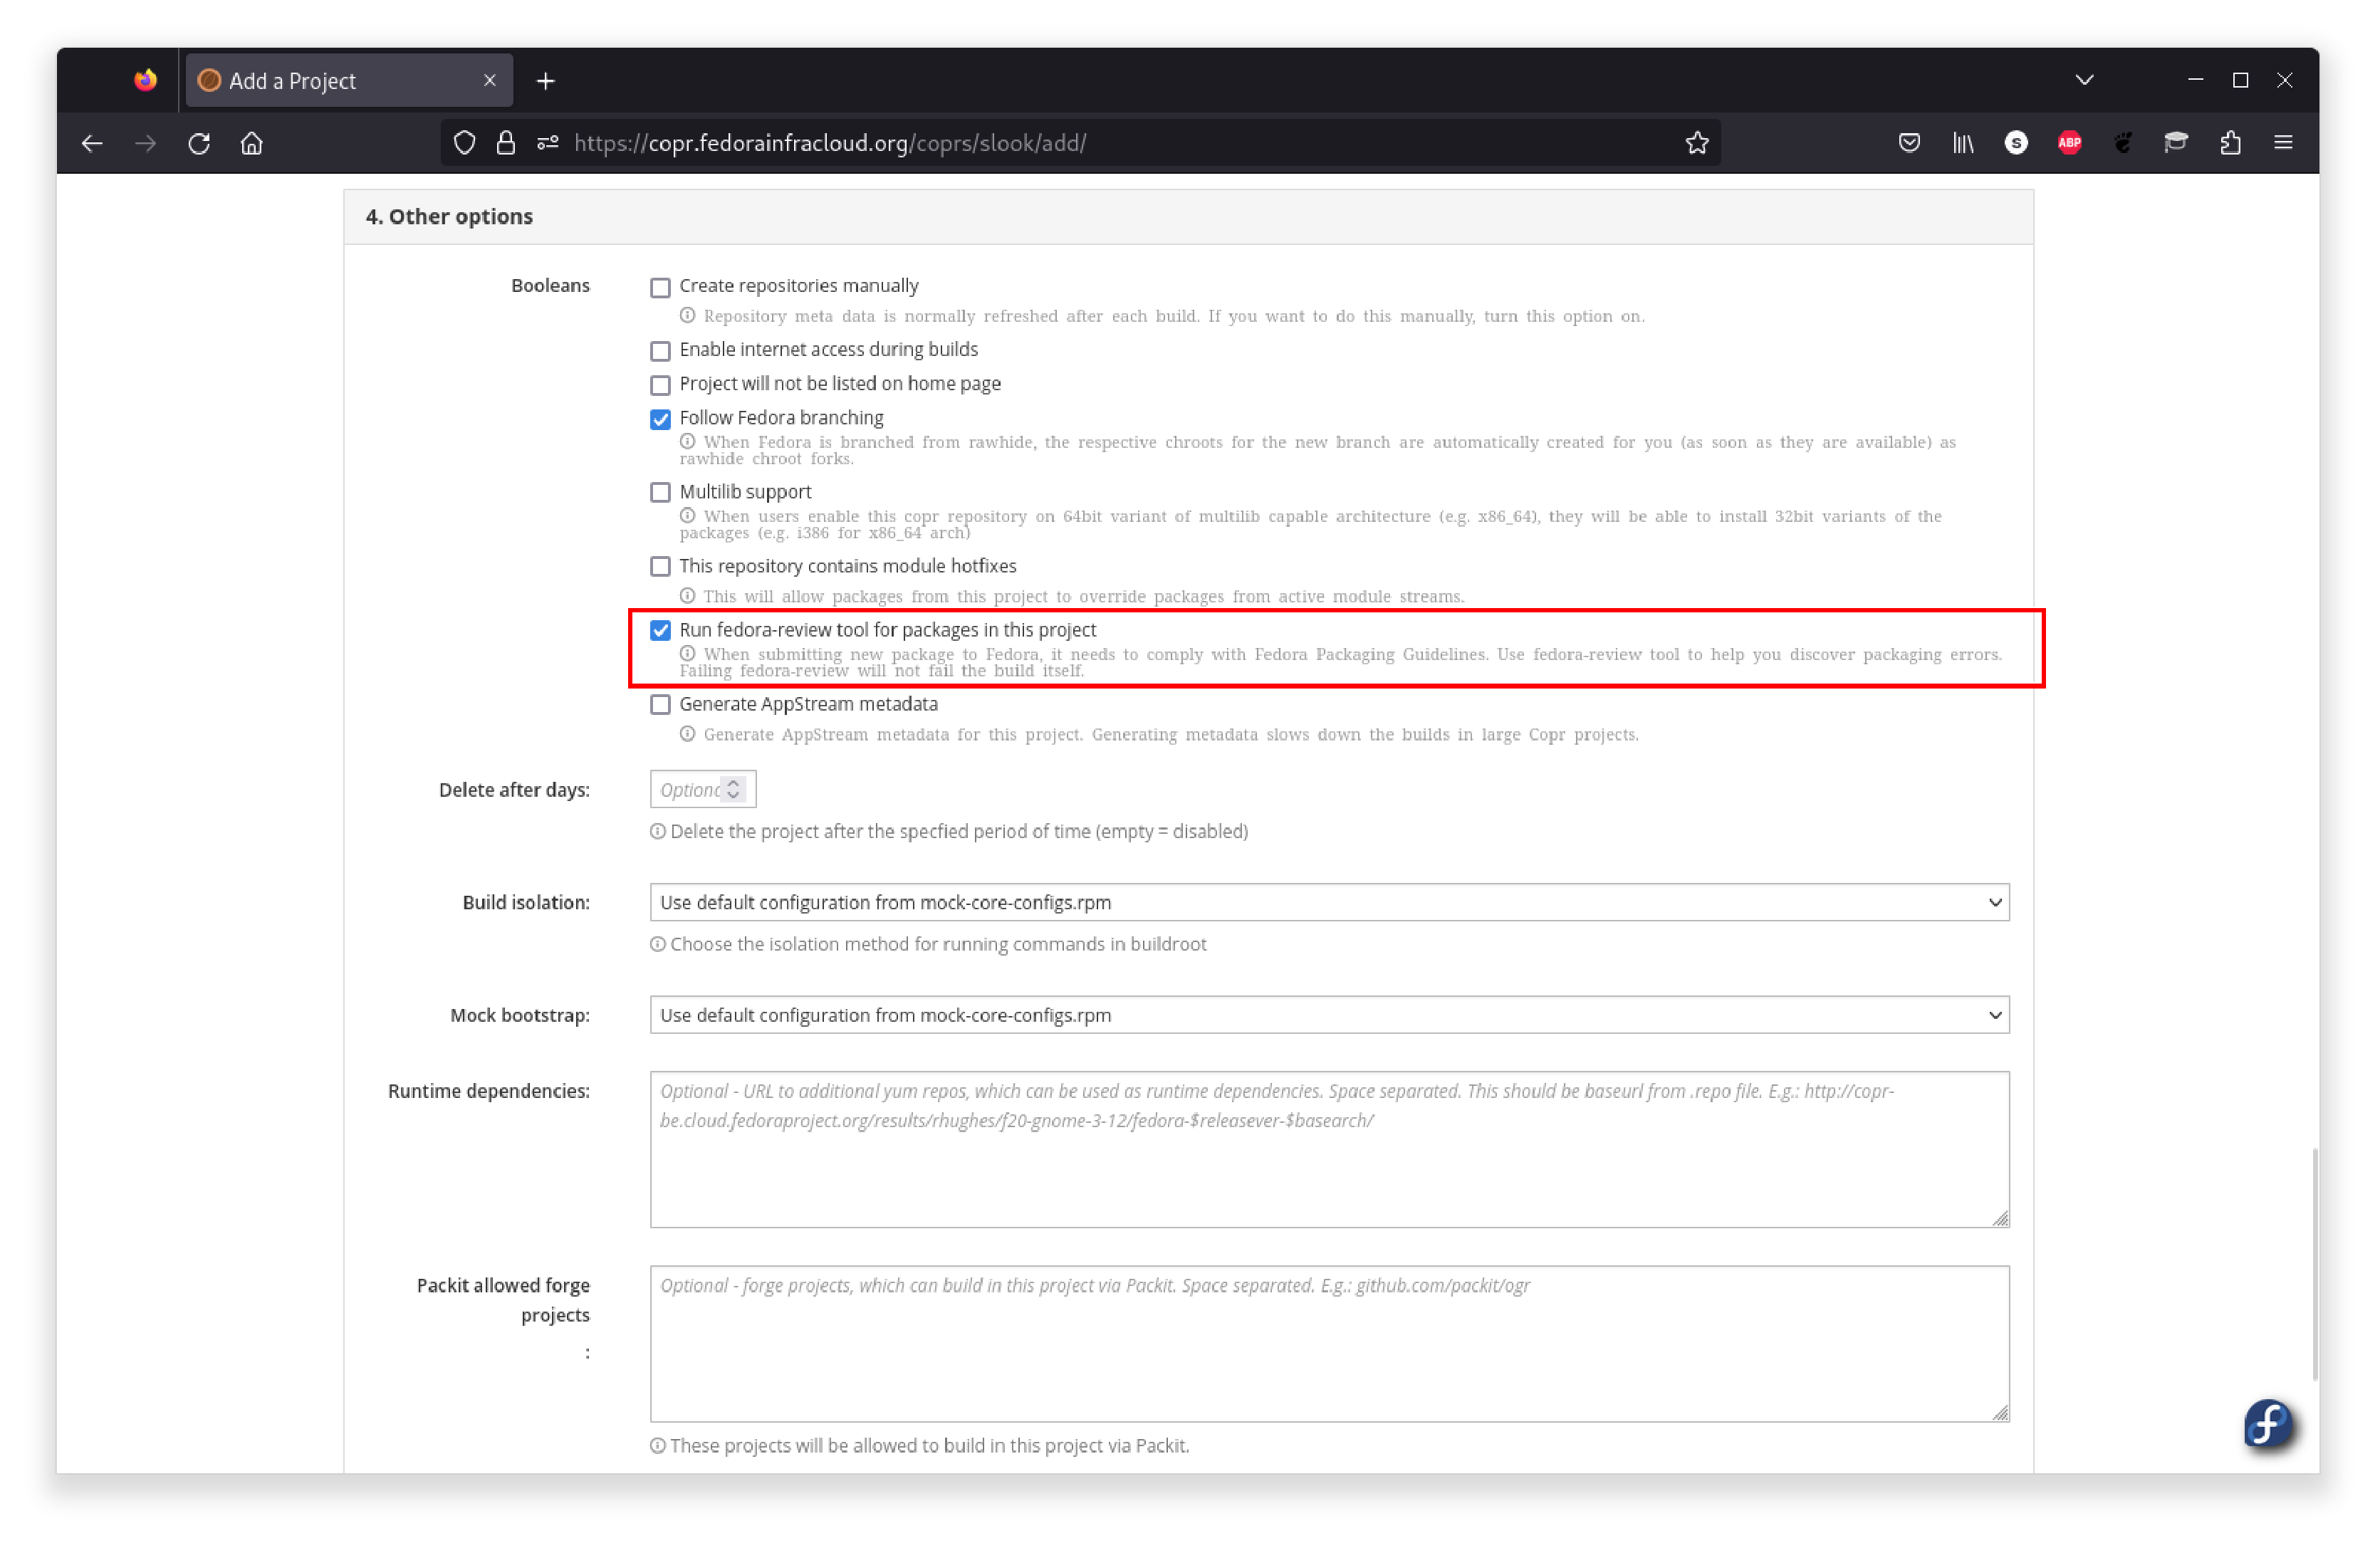
\includegraphics[width=1.0\textwidth,keepaspectratio=true,draft=\ddst]{img/rpms/copr-review.eps}
\end{center}
\newpage
\noindent After the building the RPM with the proper option, check out the results and open the corresponding information page: \\
\begin{center}
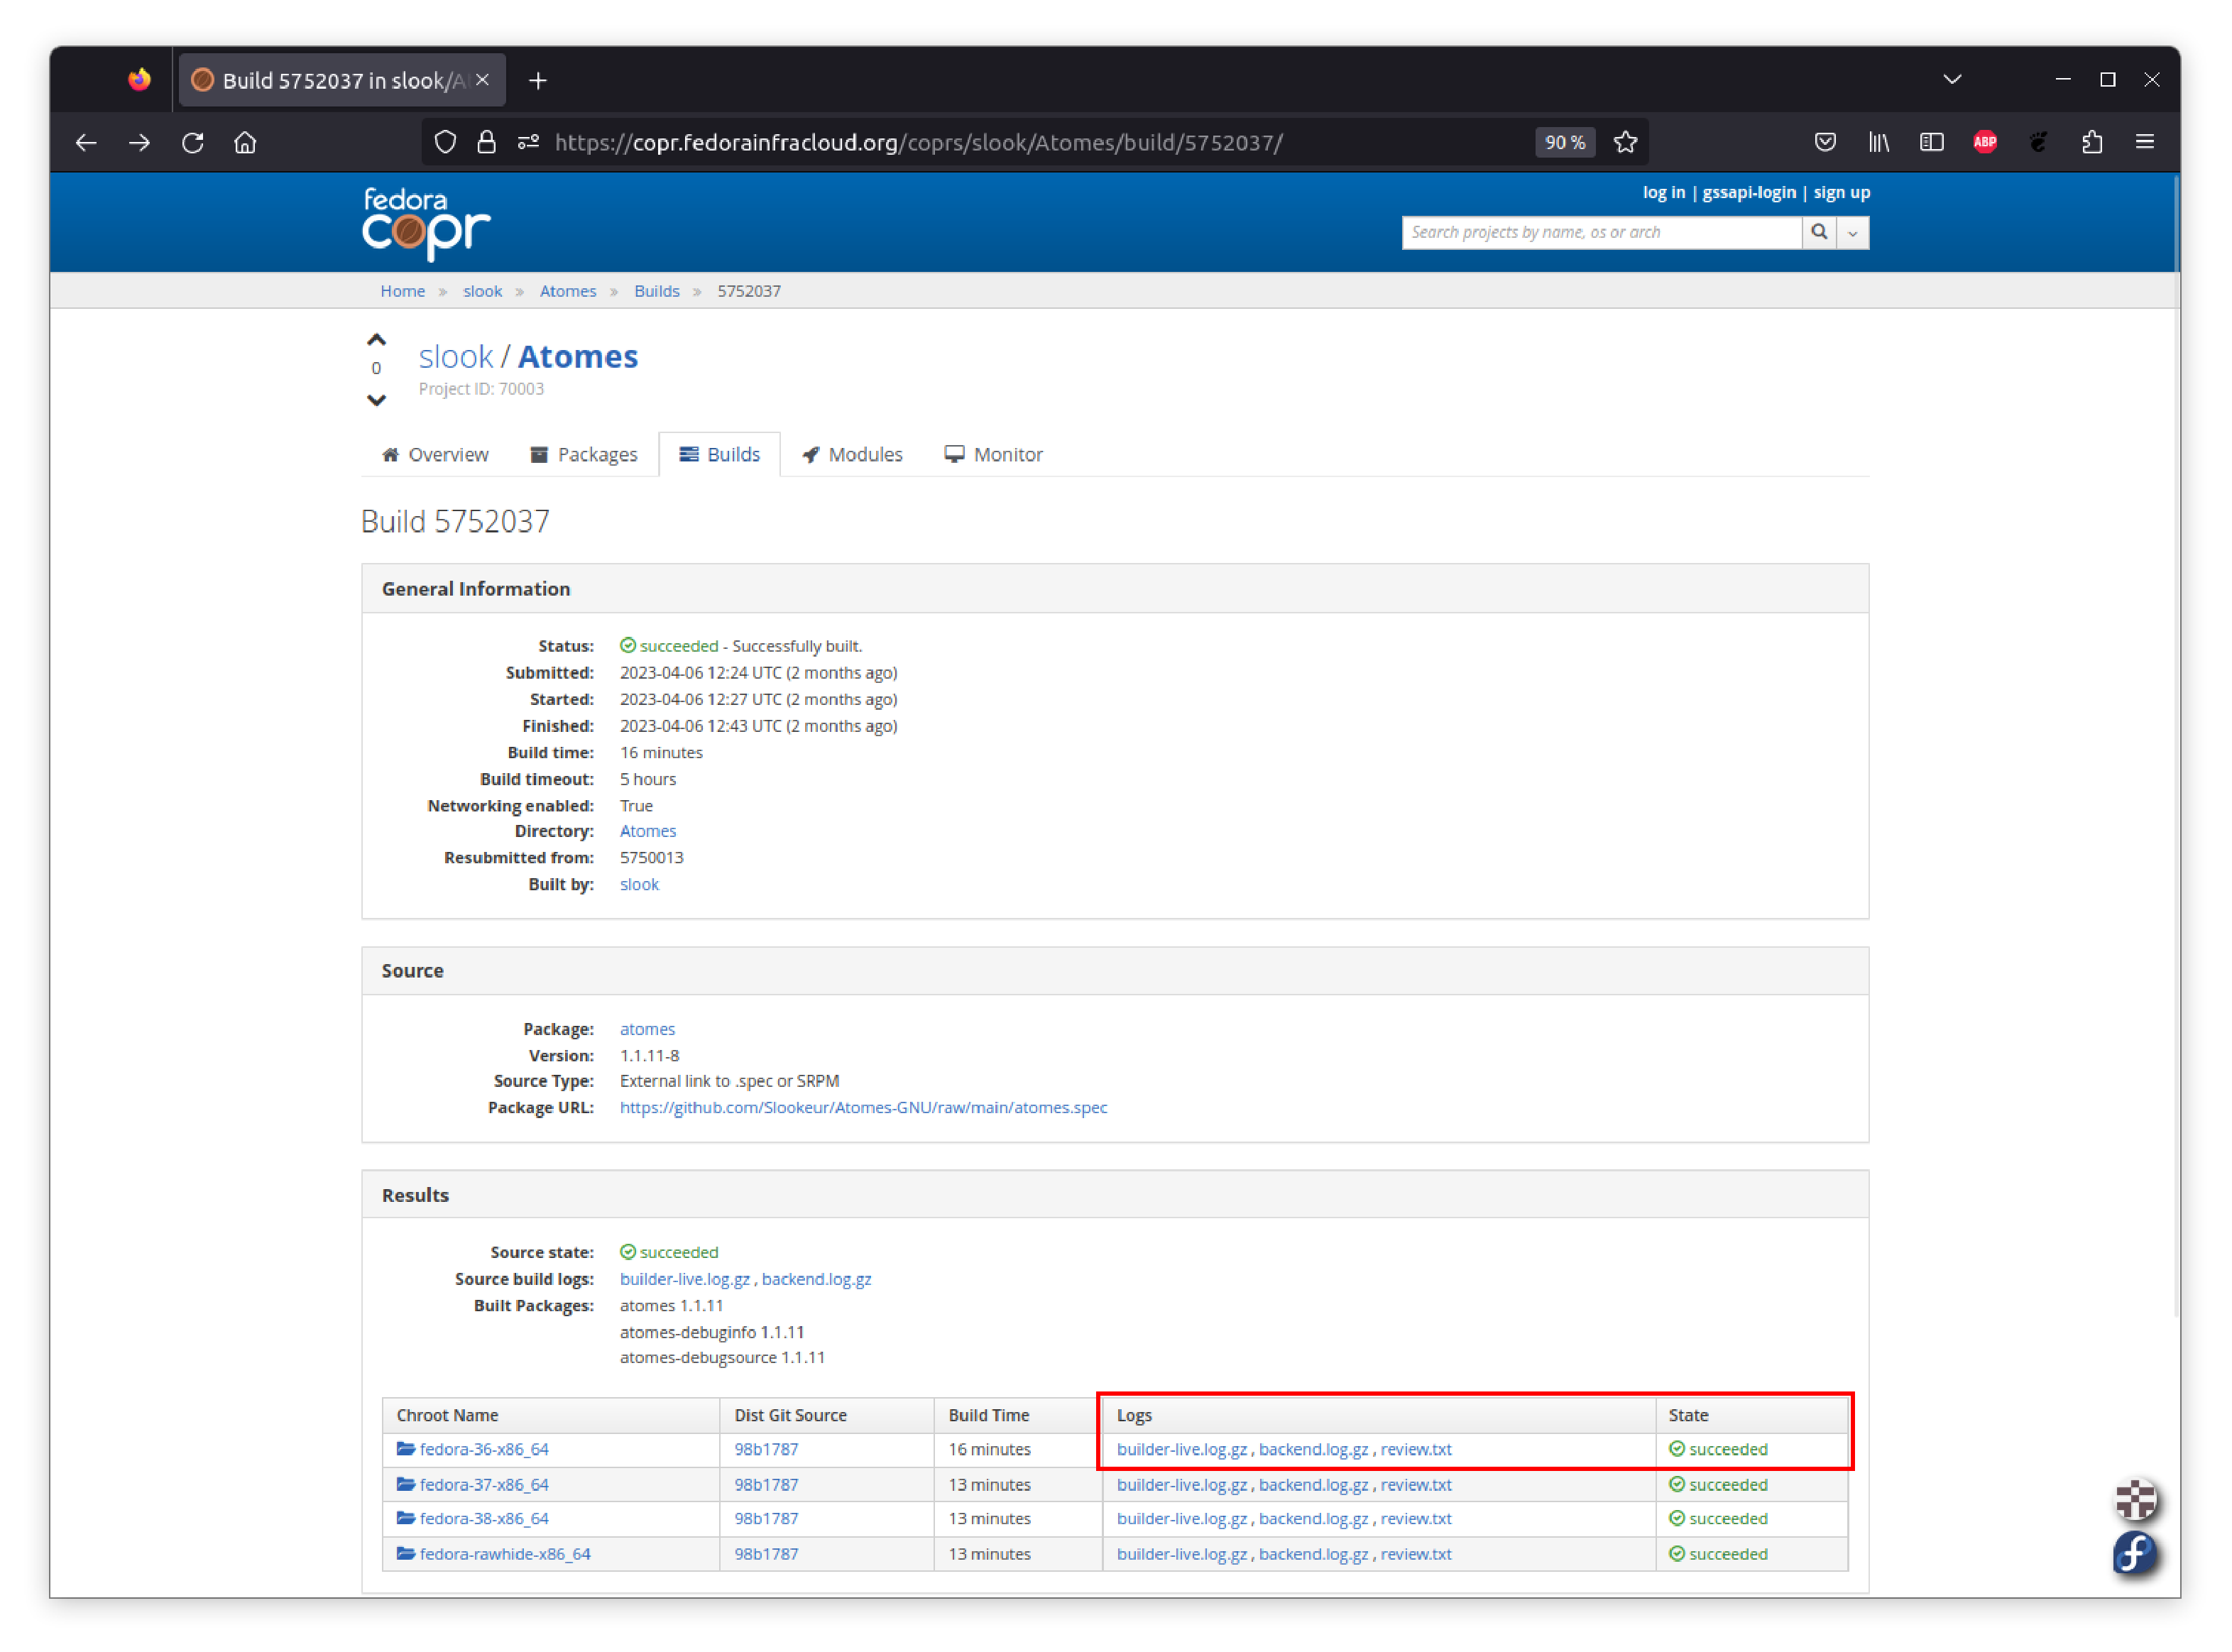
\includegraphics[width=0.8\textwidth,keepaspectratio=true,draft=\ddst]{img/rpms/copr-rev-res.eps}
\end{center}
Scroll down if needed, and in the bottom section check the "Logs" section, several files outputs of the build are provided, including a file "\texttt{review.txt}", 
click on the link to access the results of the Fedora review:
\begin{center}
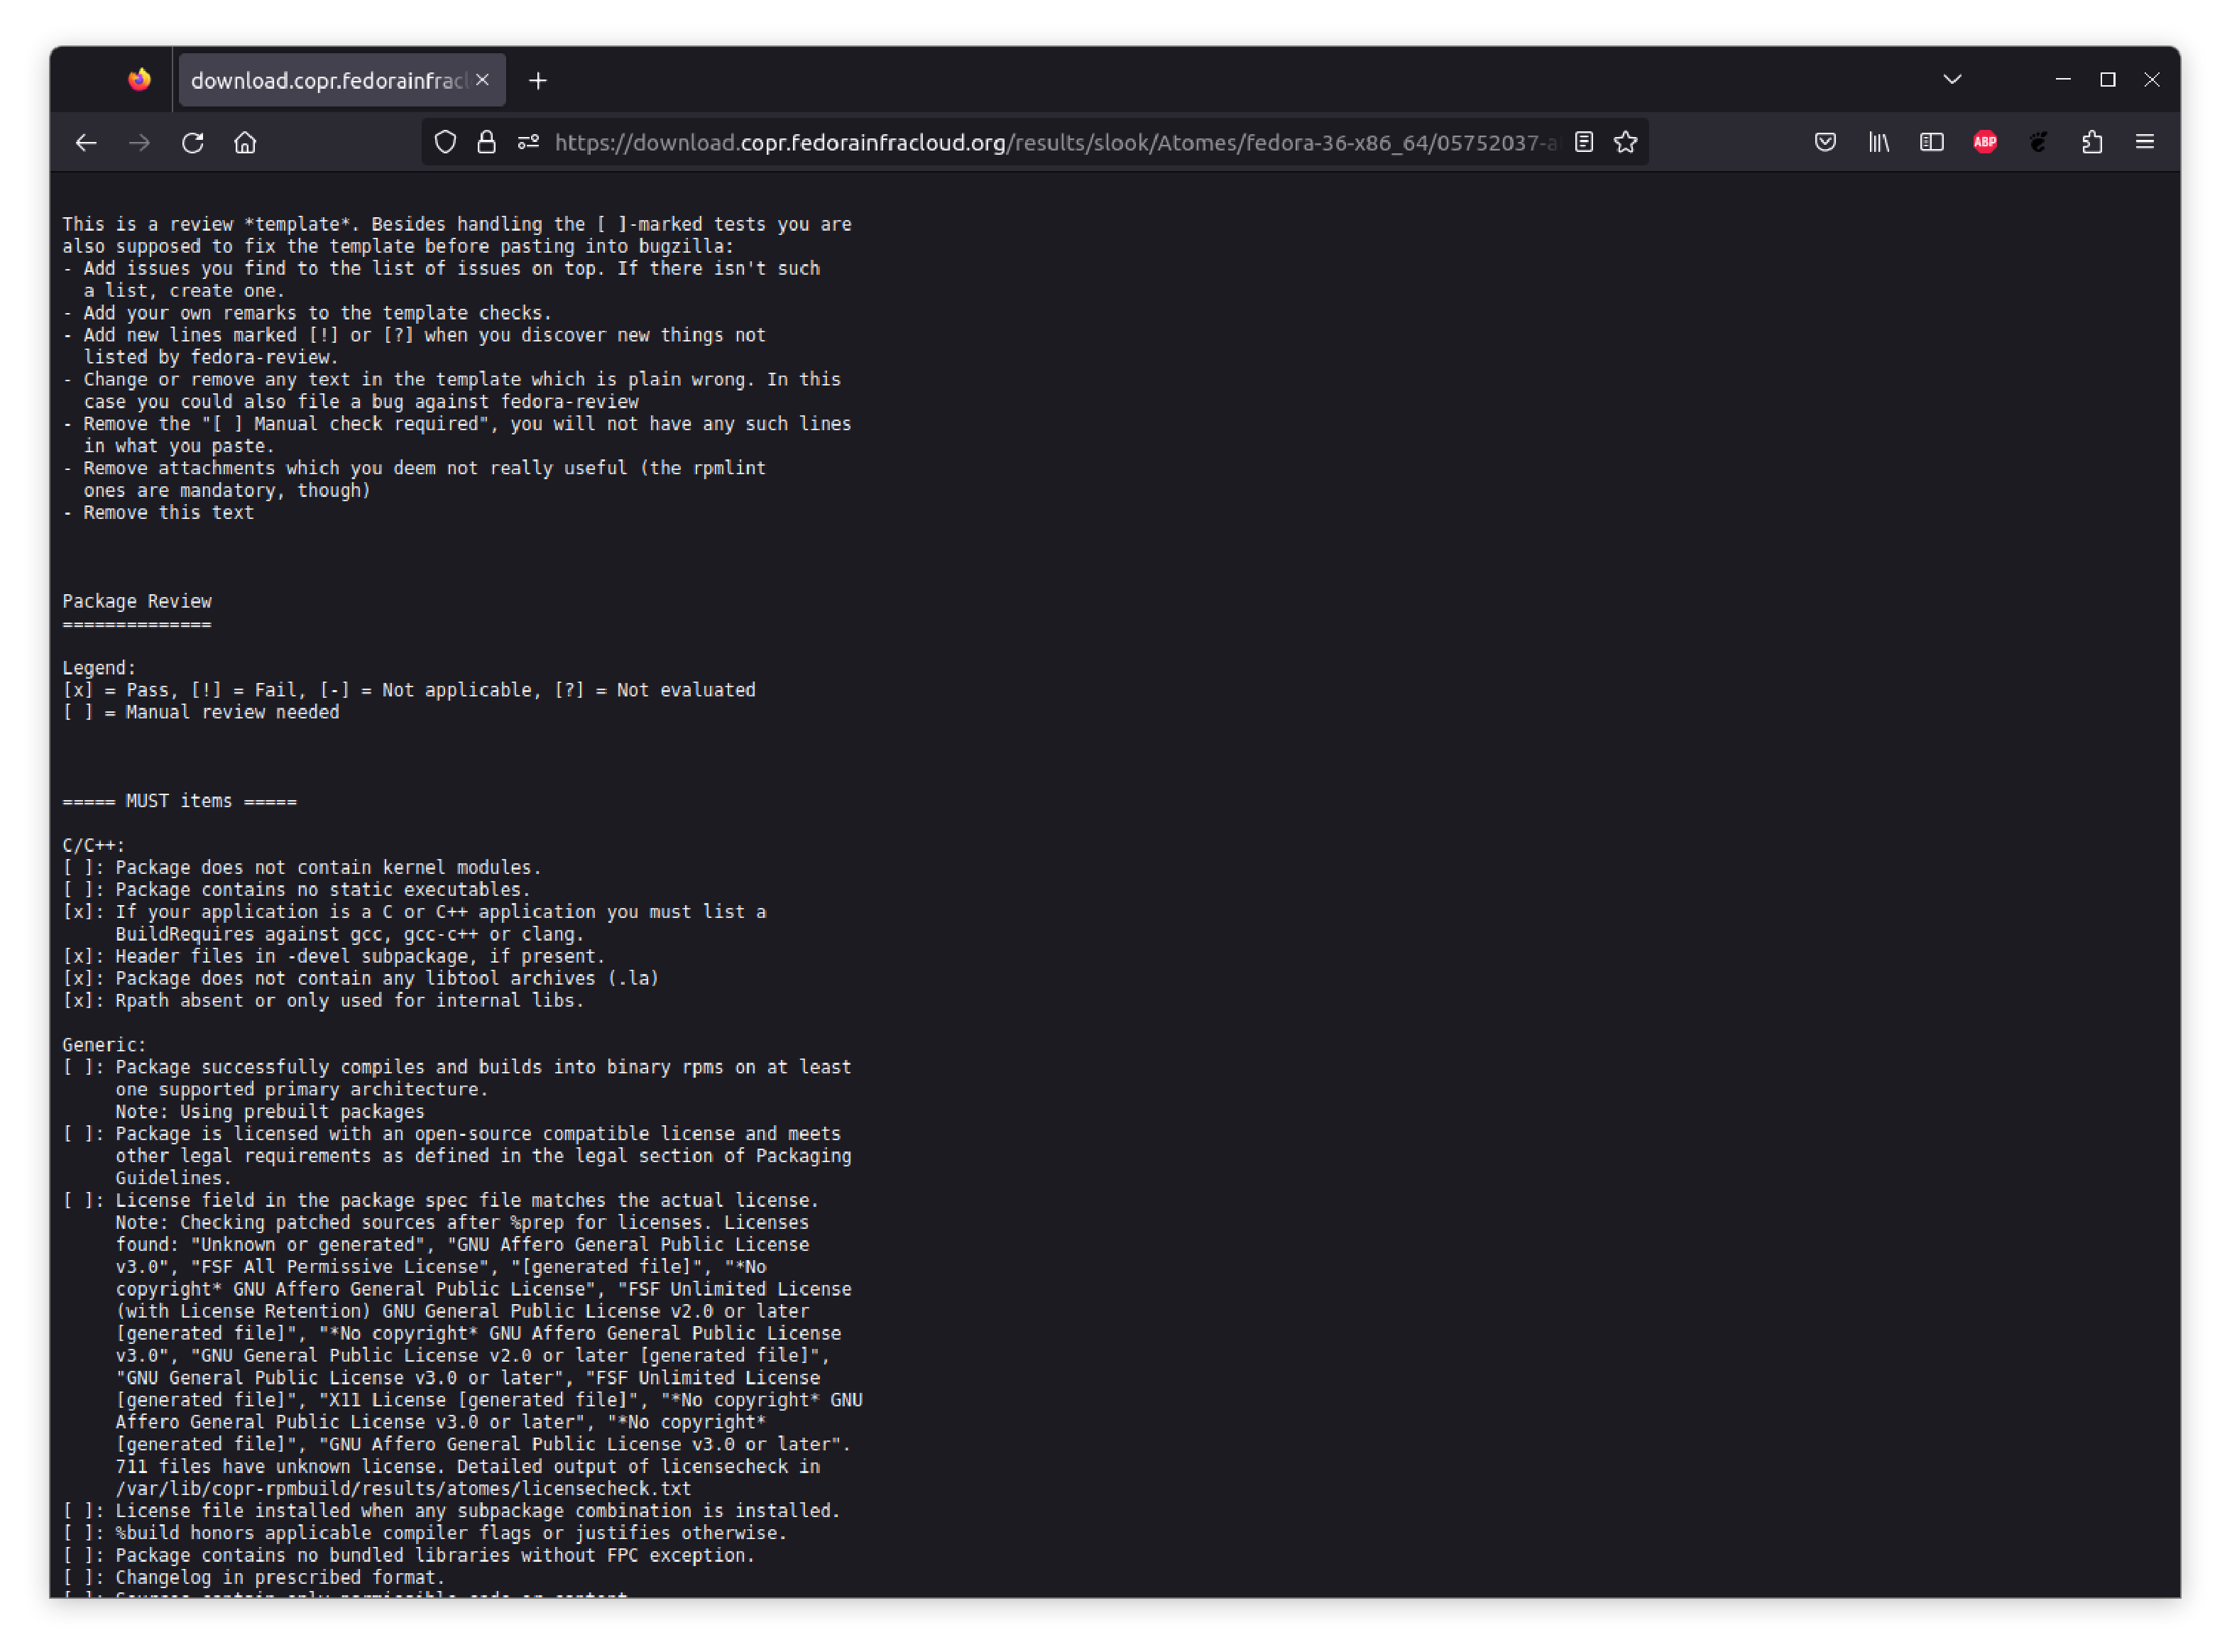
\includegraphics[width=0.8\textwidth,keepaspectratio=true,draft=\ddst]{img/rpms/copr-package-review.eps}
\end{center}

%\subsubsection{Remotely on Koji}
%\label{rkoji}
%On Koji review information are accessible following the link provide at the beginning of the output:
%\begin{script}
%\fprompt{~} \bftt{koji} \rtt{build} --sractch rawhide program-***.fc36.src.rpm
%Uploading srpm:  program-***.src.rpm
%[=================================] 100\% 00:00:01   3.14 MiB   2.54 MiB/sec
%Created task: 101830239
%Task info: \href{https://koji.fedoraproject.org/koji/taskinfo?taskID=101830239}{https://koji.fedoraproject.org/koji/taskinfo?taskID=101830239}
%\end{script}
%Simply open the link: \texttt{\href{https://koji.fedoraproject.org/koji/taskinfo?taskID=101830239}{https://koji.fedoraproject.org/koji/taskinfo?taskID=101830239}} \\[0.25cm]
%Then scroll down on this page up to the build information, select (click) on one the build architectures to check the 

\subsection{Submitting your RPM to the Fedora project}

At this point I will consider that you already prepared you own version of the RPM package, ideally following the guidelines provided in this manual. 
If not you should really take the time to prepare a first, raw, version of your RPM package. 
Doing so will at least tell the Fedora packagers, members of the Fedora community 
in charge of packaging applications, that you are willing to be part of the process, as you should. \\[0.25cm]
Ideally you should already have test build this package in Copr and / or Koji:
\begin{itemize}
\item For Copr copy the link to the package review information (see [Sec.~\ref{rcopr}]).
\item For Koji copy the address of the webpage with the build information (see [Sec.~\ref{kojib}]). 
\end{itemize}
To submit your RPM package to the Fedora project:
\begin{enumerate}
\item Create a \href{https://accounts.fedoraproject.org/}{Fedora account} (see [Sec.~\ref{coprb}]).
\item Create a \href{https://bugzilla.redhat.com}{Red Hat Bugzilla} account, with the same email used to create the Fedora account. 
%\begin{center}
%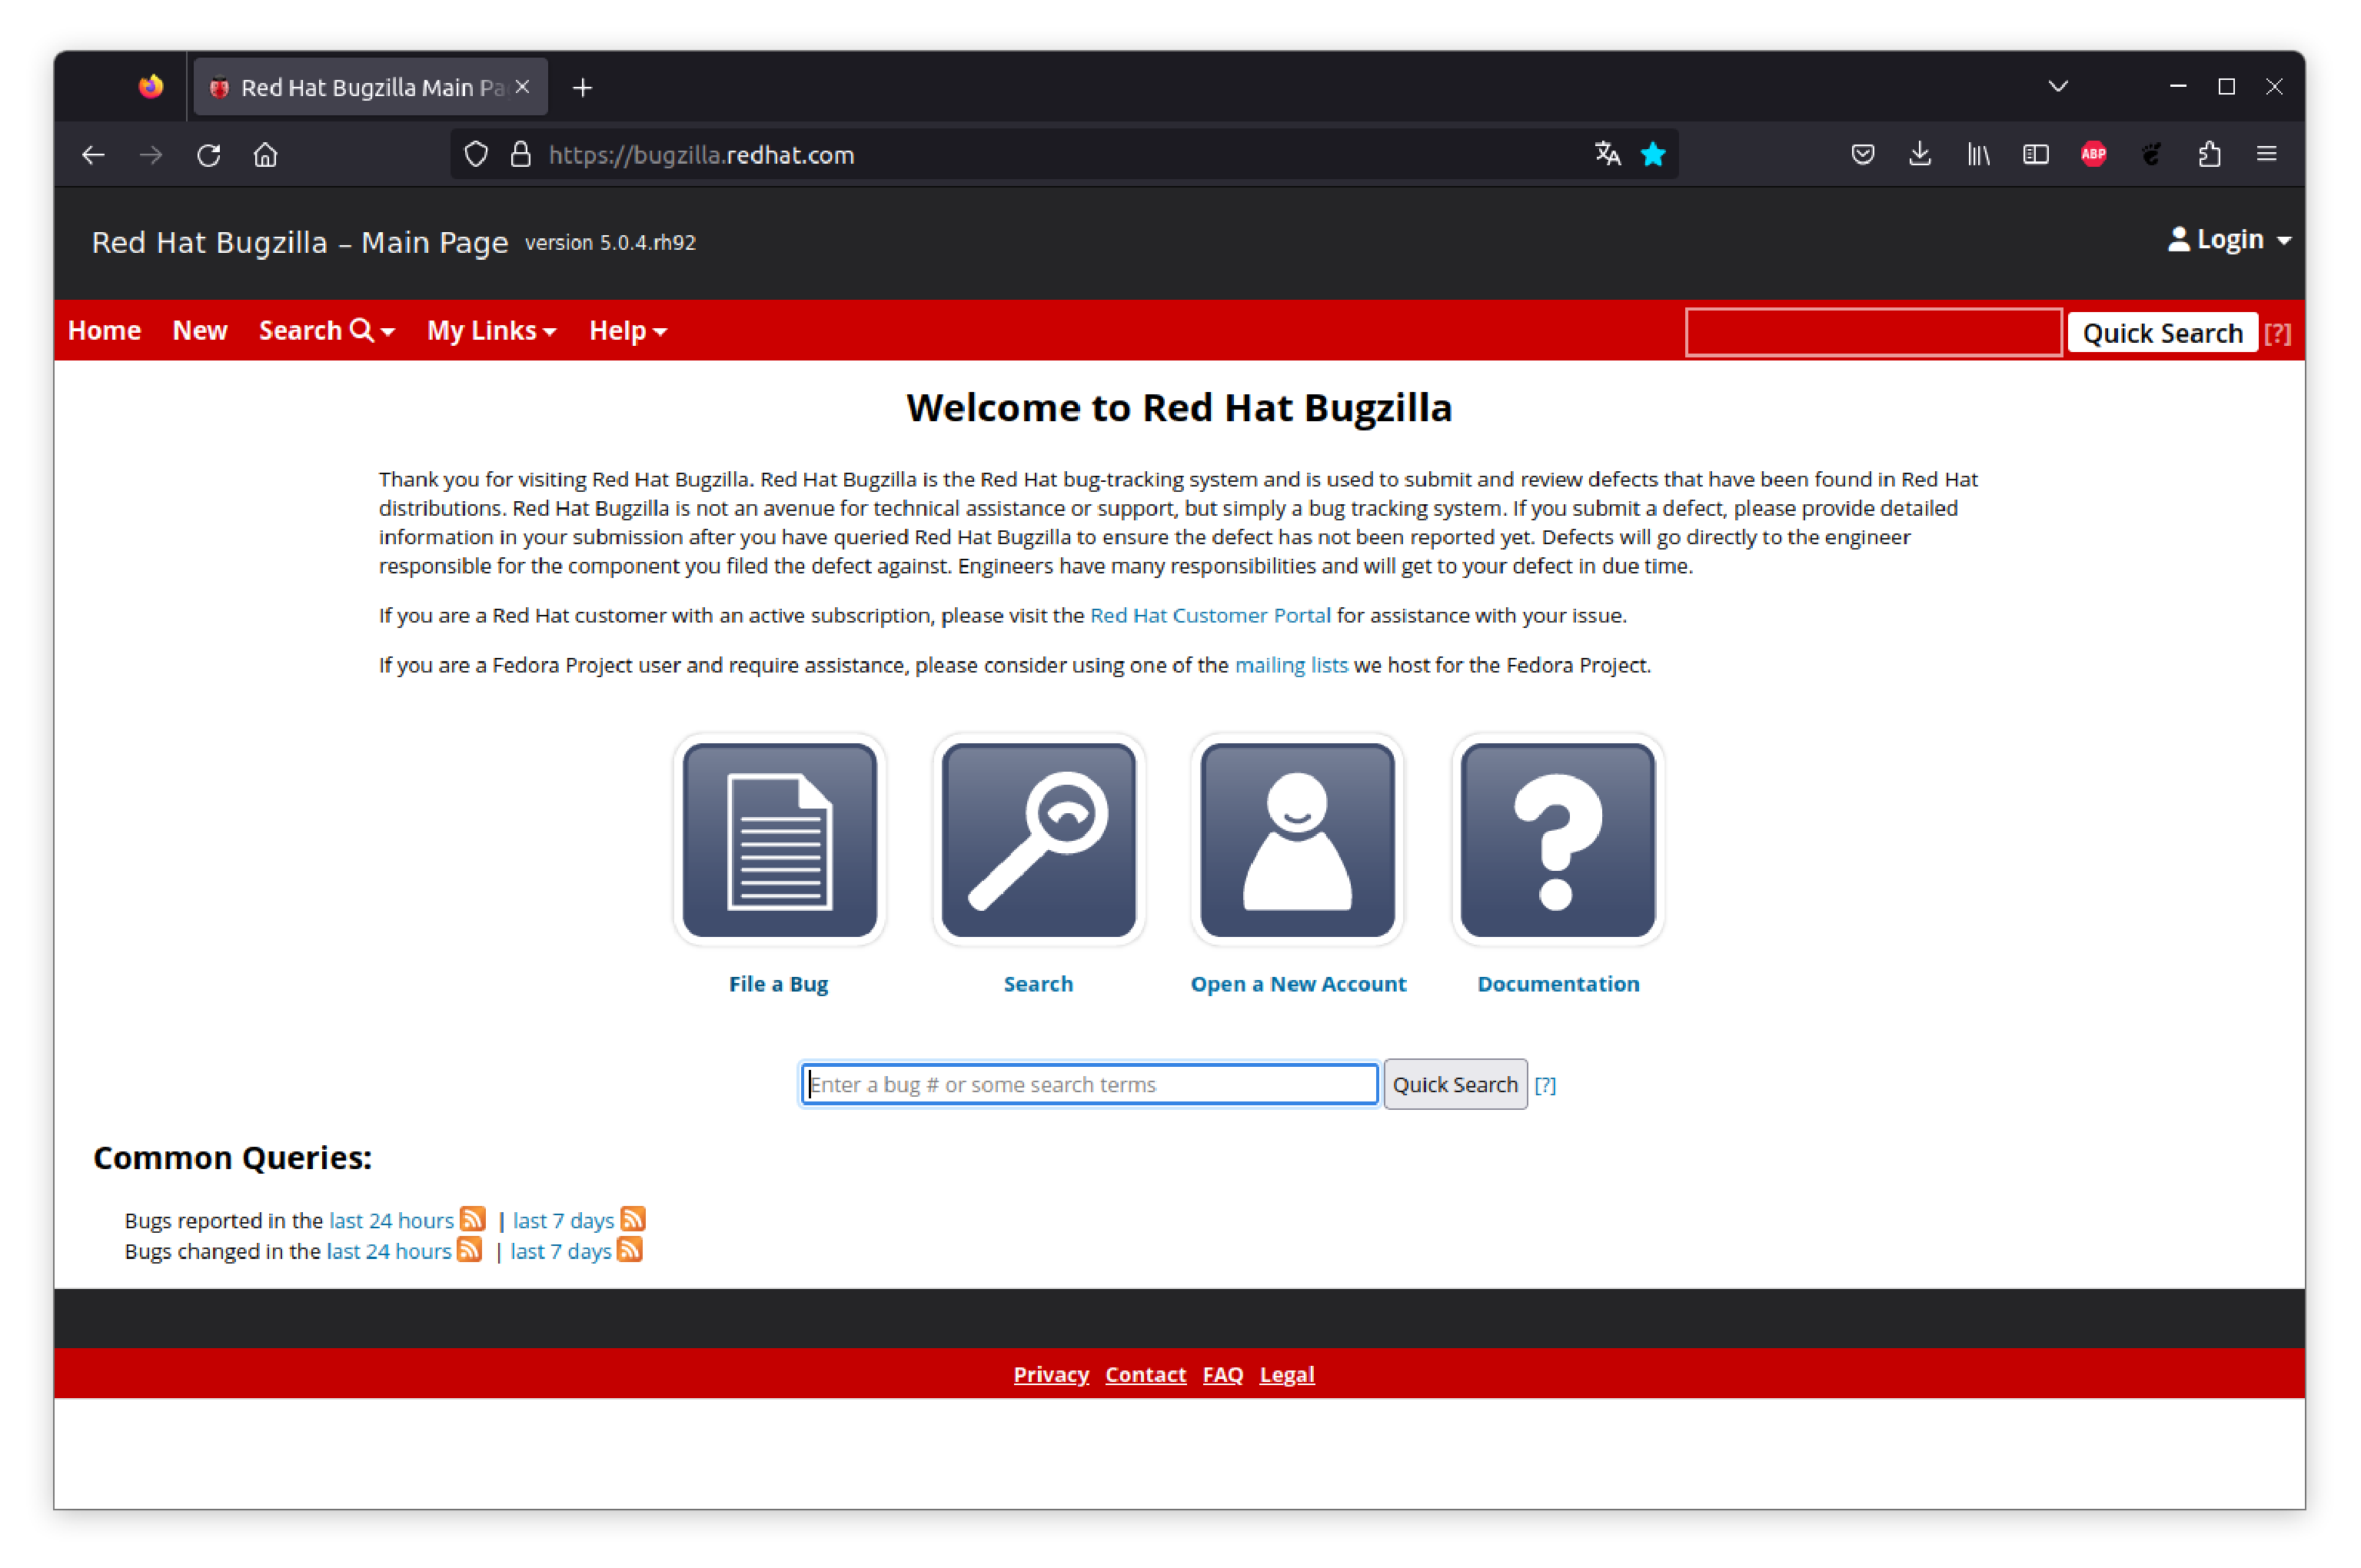
\includegraphics[width=1.0\textwidth,keepaspectratio=true,draft=\ddst]{img/rpms/bugzilla/bugzilla-0.eps}
%\end{center}
\item Create a message in \href{https://bugzilla.redhat.com/}{https://bugzilla.redhat.com/} to request the review of your package. 
\item Create a message to introduce yourself and ask to join the Fedora Package Maintainers.
%More information here: \href{https://docs.fedoraproject.org/en-US/package-maintainers/Joining\_the\_Package\_Maintainers/}{https://docs.fedoraproject.org/en-US/package-maintainers/Joining\_the\_Package\_Maintainers/}
\end{enumerate}

\subsubsection{The Red Hat Bugzilla message to request a new package review}

\begin{enumerate}
\item Login to \href{https://bugzilla.redhat.com}{Red Hat Bugzilla}
\begin{center}
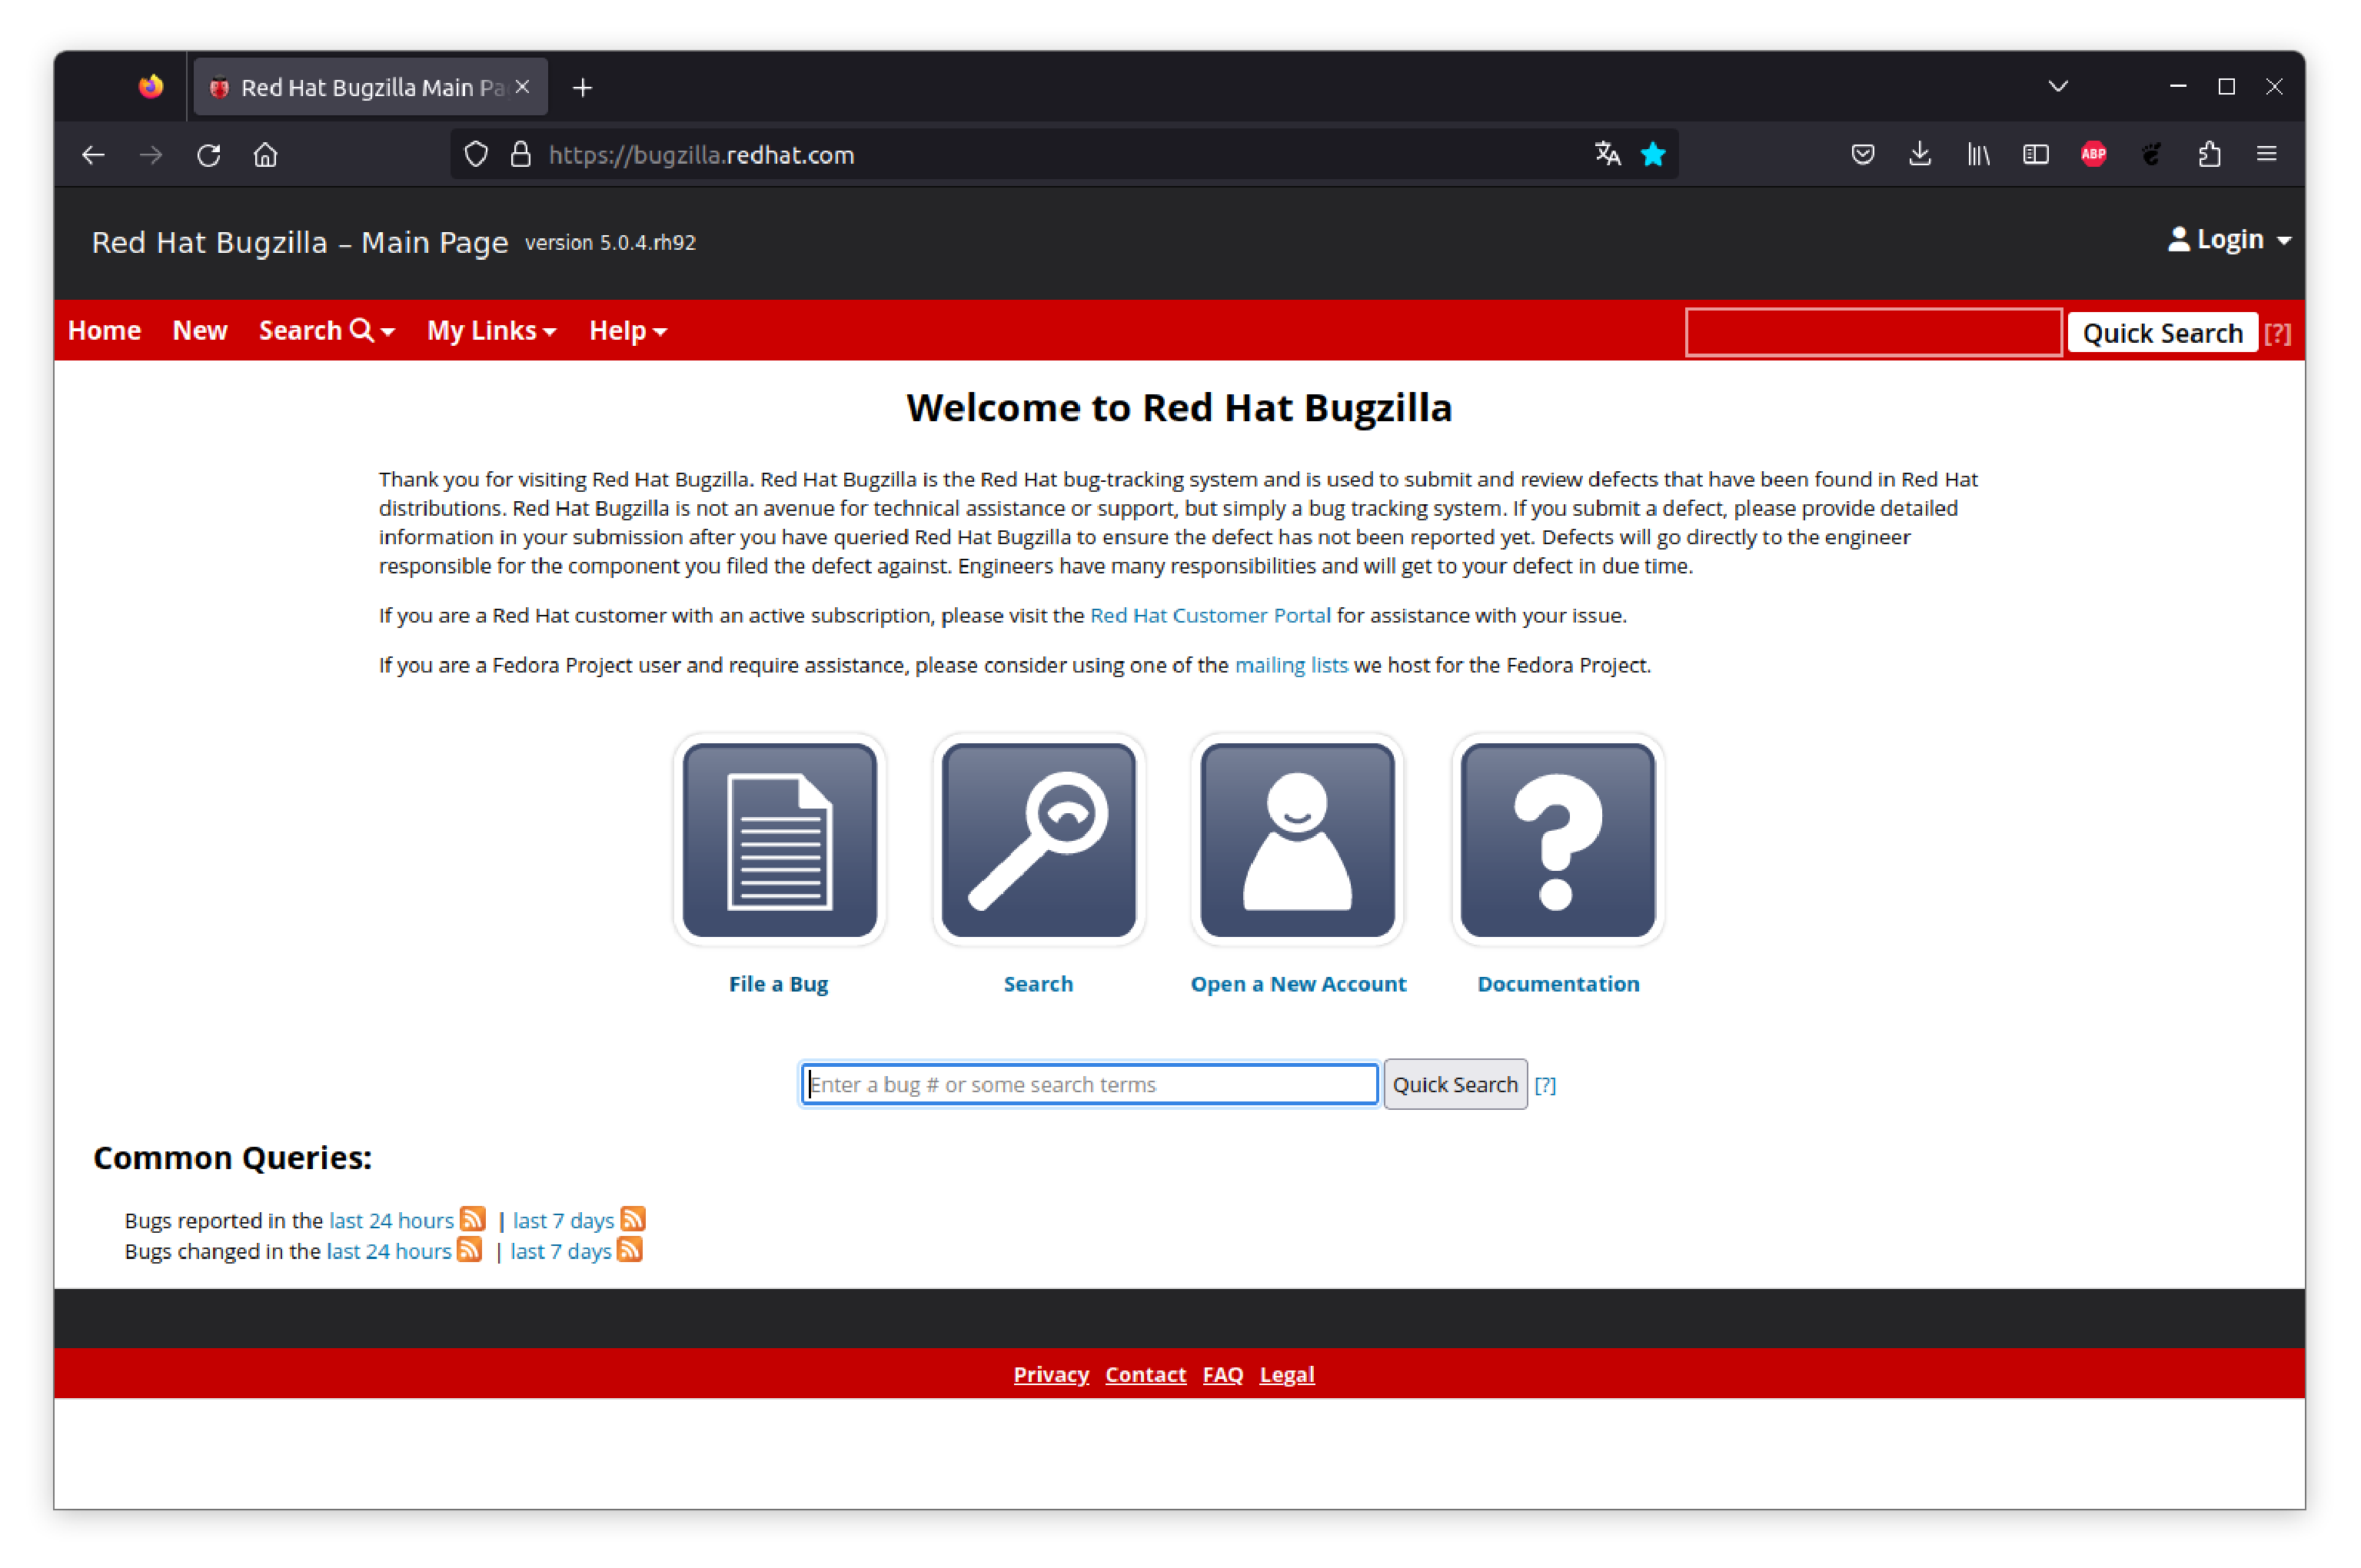
\includegraphics[width=0.9\textwidth,keepaspectratio=true,draft=\ddst]{img/rpms/bugzilla/bugzilla-0.eps}
\end{center}
The click of "File a Bug", please note that depending if you logged in using your "Fedora Account System" or a "Red Hat Bugzilla Account" the page dedicated to the preparation of the bug message might be slightly different. \\
For the sake of consistency with this tutorial I would recommend to login using the "Red Hat Bugzilla" account you just created. 
\item Then "File a Bug" and create a new message: 
\begin{itemize}
\item Click of "Fedora", then click of "Fedora" again:
\begin{center}
\hspace{-3.25cm}
\includegraphics[width=1.05\textwidth,keepaspectratio=true,draft=\ddst]{img/rpms/bugzilla/bugzilla-4.eps}
\end{center}
You are now of the interface dedicated to the preparation of the message to ask for your package to be reviewed by members of the Fedora Package Maintainers.
\item In Component select (or enter) "\texttt{Package Review}" 
\item Summary should start with:\\[0.25cm]
"\texttt{Review request: program - short description}"\\[-0.4cm]
\begin{itemize}
\item \texttt{program} is the name of your program / package.\\[0.25cm]
It is the name that will be used to create the Fedora package, and it is case sensitive, 
so choose it carefully, basically this is the keyword Fedora, and Red Hat based Linux, users will use to search for and install your program using: \\[-0.75cm]
\begin{scriptiii}
\fprompt{~} sudo dnf install prog
\end{scriptiii}
\\[-0.75cm]
\item \texttt{short description} describes its purpose in as few words as possible\\[-0.25cm] 
\end{itemize}
\item Priority, Hardware and OS should be set to "\texttt{Unspecified}" 
\item Severity should be set to "\texttt{Medium}"
\item In the message section, you can delete the "\texttt{Bug Description}" section since your are not reporting a bug, instead you are asking for help to review your new package: 
\begin{itemize}
\item In the introduction part of the message: 
\begin{itemize}
\item Introduce yourself:
\begin{itemize}
\item Real name
\item Fedora Account System username (useful for future exchanges)
\item Tell more about your work. \\[0.25cm]
Doing this professionally it is a good idea to tell Package Maintainers about your job,
indeed it is likely to help you find people in the same area of expertise, the best way to get help and to find a sponsor (see below). \\[-0.25cm] 
\item Introduce briefly your software\\[-0.25cm]
\end{itemize}
\item Provide a link to the repository of the "\texttt{.spec}" file used to create the RPM. 
\item Provide a link to the last SRPM (source RPM).
\item Ideally provide a link to the last successful Koji (or Copr) build. 
\item State that you need a sponsor: this is mandatory for your first package. \\[0.25cm]
A sponsor is an official member of the Fedora Package Maintainers experienced enough to ensure that your package 
is properly prepared, and who can validate its integration to the Fedora ecosystem. 
Your sponsor will also register you as an official Fedora Package Maintainer for your package. \\
\end{itemize}
\item In the Description part of the message:
\begin{itemize}
\item Describe your program with details. 
\item Describe the interest of the program for the community.
\end{itemize}
\end{itemize}
\end{itemize}
\newpage
\item Test the information your provided in your bug "Package review" message: \\[0.25cm]
Once the email has been sent you will receive a link to a webpage hosting the entire discussion on \href{https://bugzilla.redhat.com}{Red Hat Bugzilla} at the address: \\[0.25cm]
\texttt{https://bugzilla.redhat.com/show\_bug.cgi?id=}\dctt{???????} \\[0.25cm]
\noindent Where \dctt{???????} is the bug message id number that you will find on the email you received and on the webpage hosting the discussion. \\
The information provided in your bug message can be tested by other Fedora packagers using the \bftt{fedora-review} command: 
\begin{scripti}
\fprompt{~} \bftt{fedora-review} \bftt{-b} \dctt{???????}
\end{scripti}
\\[-0.75cm]
\noindent \bftt{fedora-review} then retrieves the "\texttt{.spec}" file from the address provided in the bug message to build and test your package. 
Make sure that your package can be built like this because it is likely how official Fedora packagers will try to build and test it. \\
Note that you can edit your messages, including the first one, on this webpage to correct any information if required. 
\end{enumerate}

\subsubsection{Joining the Fedora Package Maintainers}

In the same time you need to join the Fedora Package Maintainers, so that you would later on be able to manage your package from the official Fedora repository. 
The next lines basically follow the dedicated tutorial: \href{https://docs.fedoraproject.org/en-US/package-maintainers/Joining\_the\_Package\_Maintainers/}{Join the Package Maintainers}
\begin{enumerate}
\item Join the following Fedora mailing lists:
\begin{itemize}
\item The \href{https://lists.fedoraproject.org/archives/list/devel@lists.fedoraproject.org/}{Fedora devel} list 
\item The \href{https://lists.fedoraproject.org/admin/lists/devel-announce@lists.fedoraproject.org/}{Fedora devel-announce} list 
\item The \href{https://lists.fedoraproject.org/admin/lists/packaging@lists.fedoraproject.org/}{Fedora packaging} list 
\end{itemize}
\item Send an email to \href{mailto:devel@lists.fedoraproject.org}{devel@lists.fedoraproject.org} to introduce yourself and your package. \\[0.25cm]
You should now introduce yourself to the community, the primary purpose of this is to begin the process of building trust 
by allowing the Fedora community members to get to know you a bit more. 
In order to establish a level of trust between yourself and the other members of the project use your real name, describe your motivations, 
and a description of the software your are submitted for review. \\[0.25cm]
The email subject should be: \texttt{Self Introduction: }\bftt{Your Name}
\end{enumerate}

\newpage
\subsubsection{After that: the next steps}

The next steps of the process are not up to you, or not entirely anyway. \\
As soon as both personal introduction and bug message have been sent, the community feedback is required for your package 
to go further. 
Packager(s) will look into your bug message to test your package, they will likely use the \bftt{fedora-review} tool
to build and test it, as introduced previously, so make sure that the build works like this. \\
The more your ensured that your package follows the official Fedora packaging guidelines (check the output provided by \bftt{fedora-review} or Copr), 
the more easily your package will be accepted. \\[0.25cm] 
The most complicated part is likely to find a sponsor, an official Fedora package maintainer experienced enough to be allowed to register new package and their maintainer. 
This is done via exchanges with the Fedora package maintainer community, here are some advise: 
\begin{itemize}
\item The process can take time: be patient !
\item Search for people that could be interested by your software in the community: remember that a good introduction is the best starting point !
\item When you have someone to talk to, ask what to do to help: be part of the process all the way through !
\end{itemize}

%\noindent Some stuff to be added here about:
%\begin{itemize}
%\item Pagure: why did I need to create a project on \href{https://pagure.io/dashboard/projects}{Pagure} ? 
%\item The confirmation email for the project creation on \href{https://src.fedoraproject.org}{https://src.fedoraproject.org}
%\item More can be find on the package review process here: \href{https://docs.fedoraproject.org/en-US/package-maintainers/Package\_Review\_Process/}{Package Review Process}
%\end{itemize}

\newpage
\subsection{Managing your official RPM package for the Fedora project}

At this stage I will assume that: 
\begin{itemize}
\item Your RPM package has been approved by your mentor
\item You are now an official member of the Fedora Package Maintainers
\end{itemize}
At first you need to get familiar with the Fedora tools at your disposal to help you update and distribute your package: 
\begin{itemize}
\item The source repository of all Fedora packages: \href{https://src.fedoraproject.org}{https://src.fedoraproject.org}  
\item The update system for Fedora packages, Bodhi: \href{https://bodhi.fedoraproject.org}{https://bodhi.fedoraproject.org}
\end{itemize}
The update process of a Fedora package can be decomposed in 3 steps:
\begin{enumerate}
\item Request an official \href{https://pagure.io/settings/token/new}{Pagure.io api token} on \href{https://pagure.io}{https://pagure.io}
\item Creating the official repository for your package on \href{https://src.fedoraproject.org}{https://src.fedoraproject.org}
\item Uploading new package sources and / or "\texttt{.spec}" file to the official repository
\item Building the new package using the update(s)
\item Requesting for the new built(s) to update the package in the official repositories
\end{enumerate}

\subsubsection{Request an official \href{https://pagure.io/settings/token/new}{Pagure.io api token} on \href{https://pagure.io/}{Pagure}}

When your package passes the review comes the time to request an official Fedora Git repository for it. 
Before doing so, you will need a \href{https://pagure.io/settings/token/new}{Pagure.io api token} token that you can obtain from the \href{https://pagure.io/}{Pagure} website. \\ 
\href{https://pagure.io/}{Pagure} is an Open Source software code hosting system for the Fedora project: 
\begin{center}
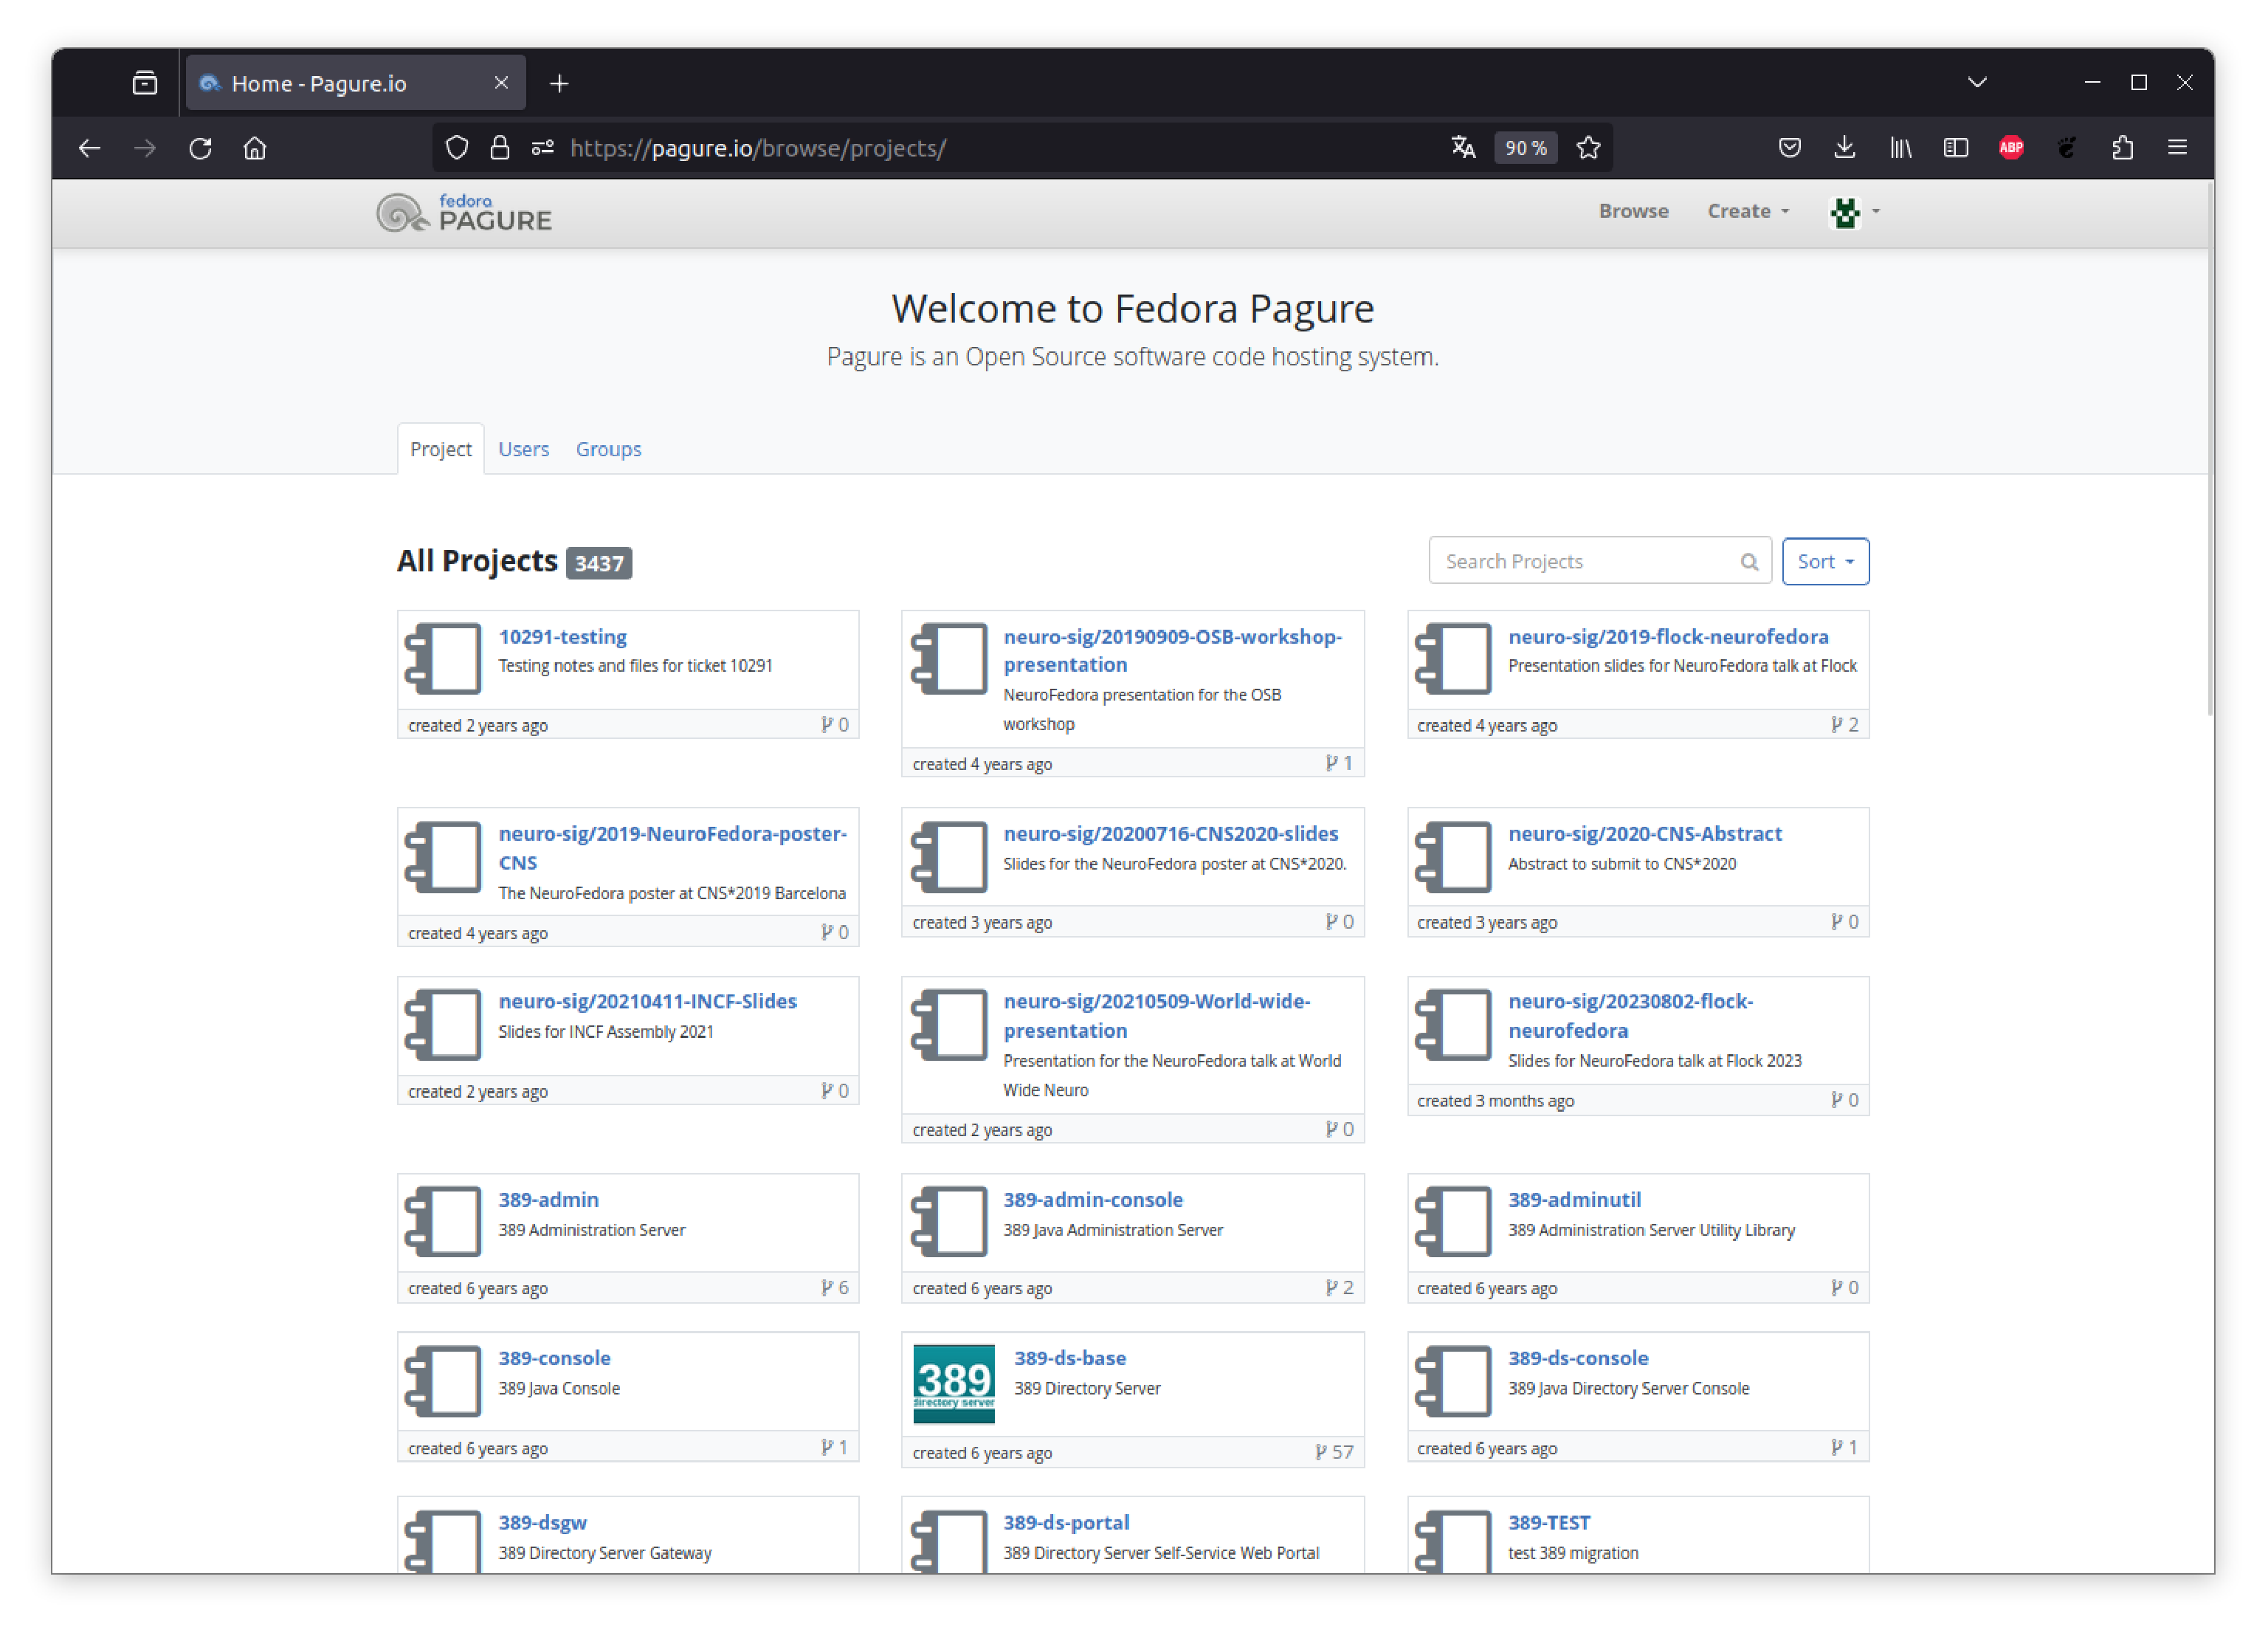
\includegraphics[width=0.75\textwidth,keepaspectratio=true,draft=\ddst]{img/rpms/pagure/pagure-0.eps}
\end{center}
\begin{enumerate}
\item On \href{https://pagure.io/}{Pagure} login using your Fedora Account credentials
\item Create a new ticket ACL: \href{https://pagure.io/settings/token/new}{https://pagure.io/settings/token/new}
\begin{center}
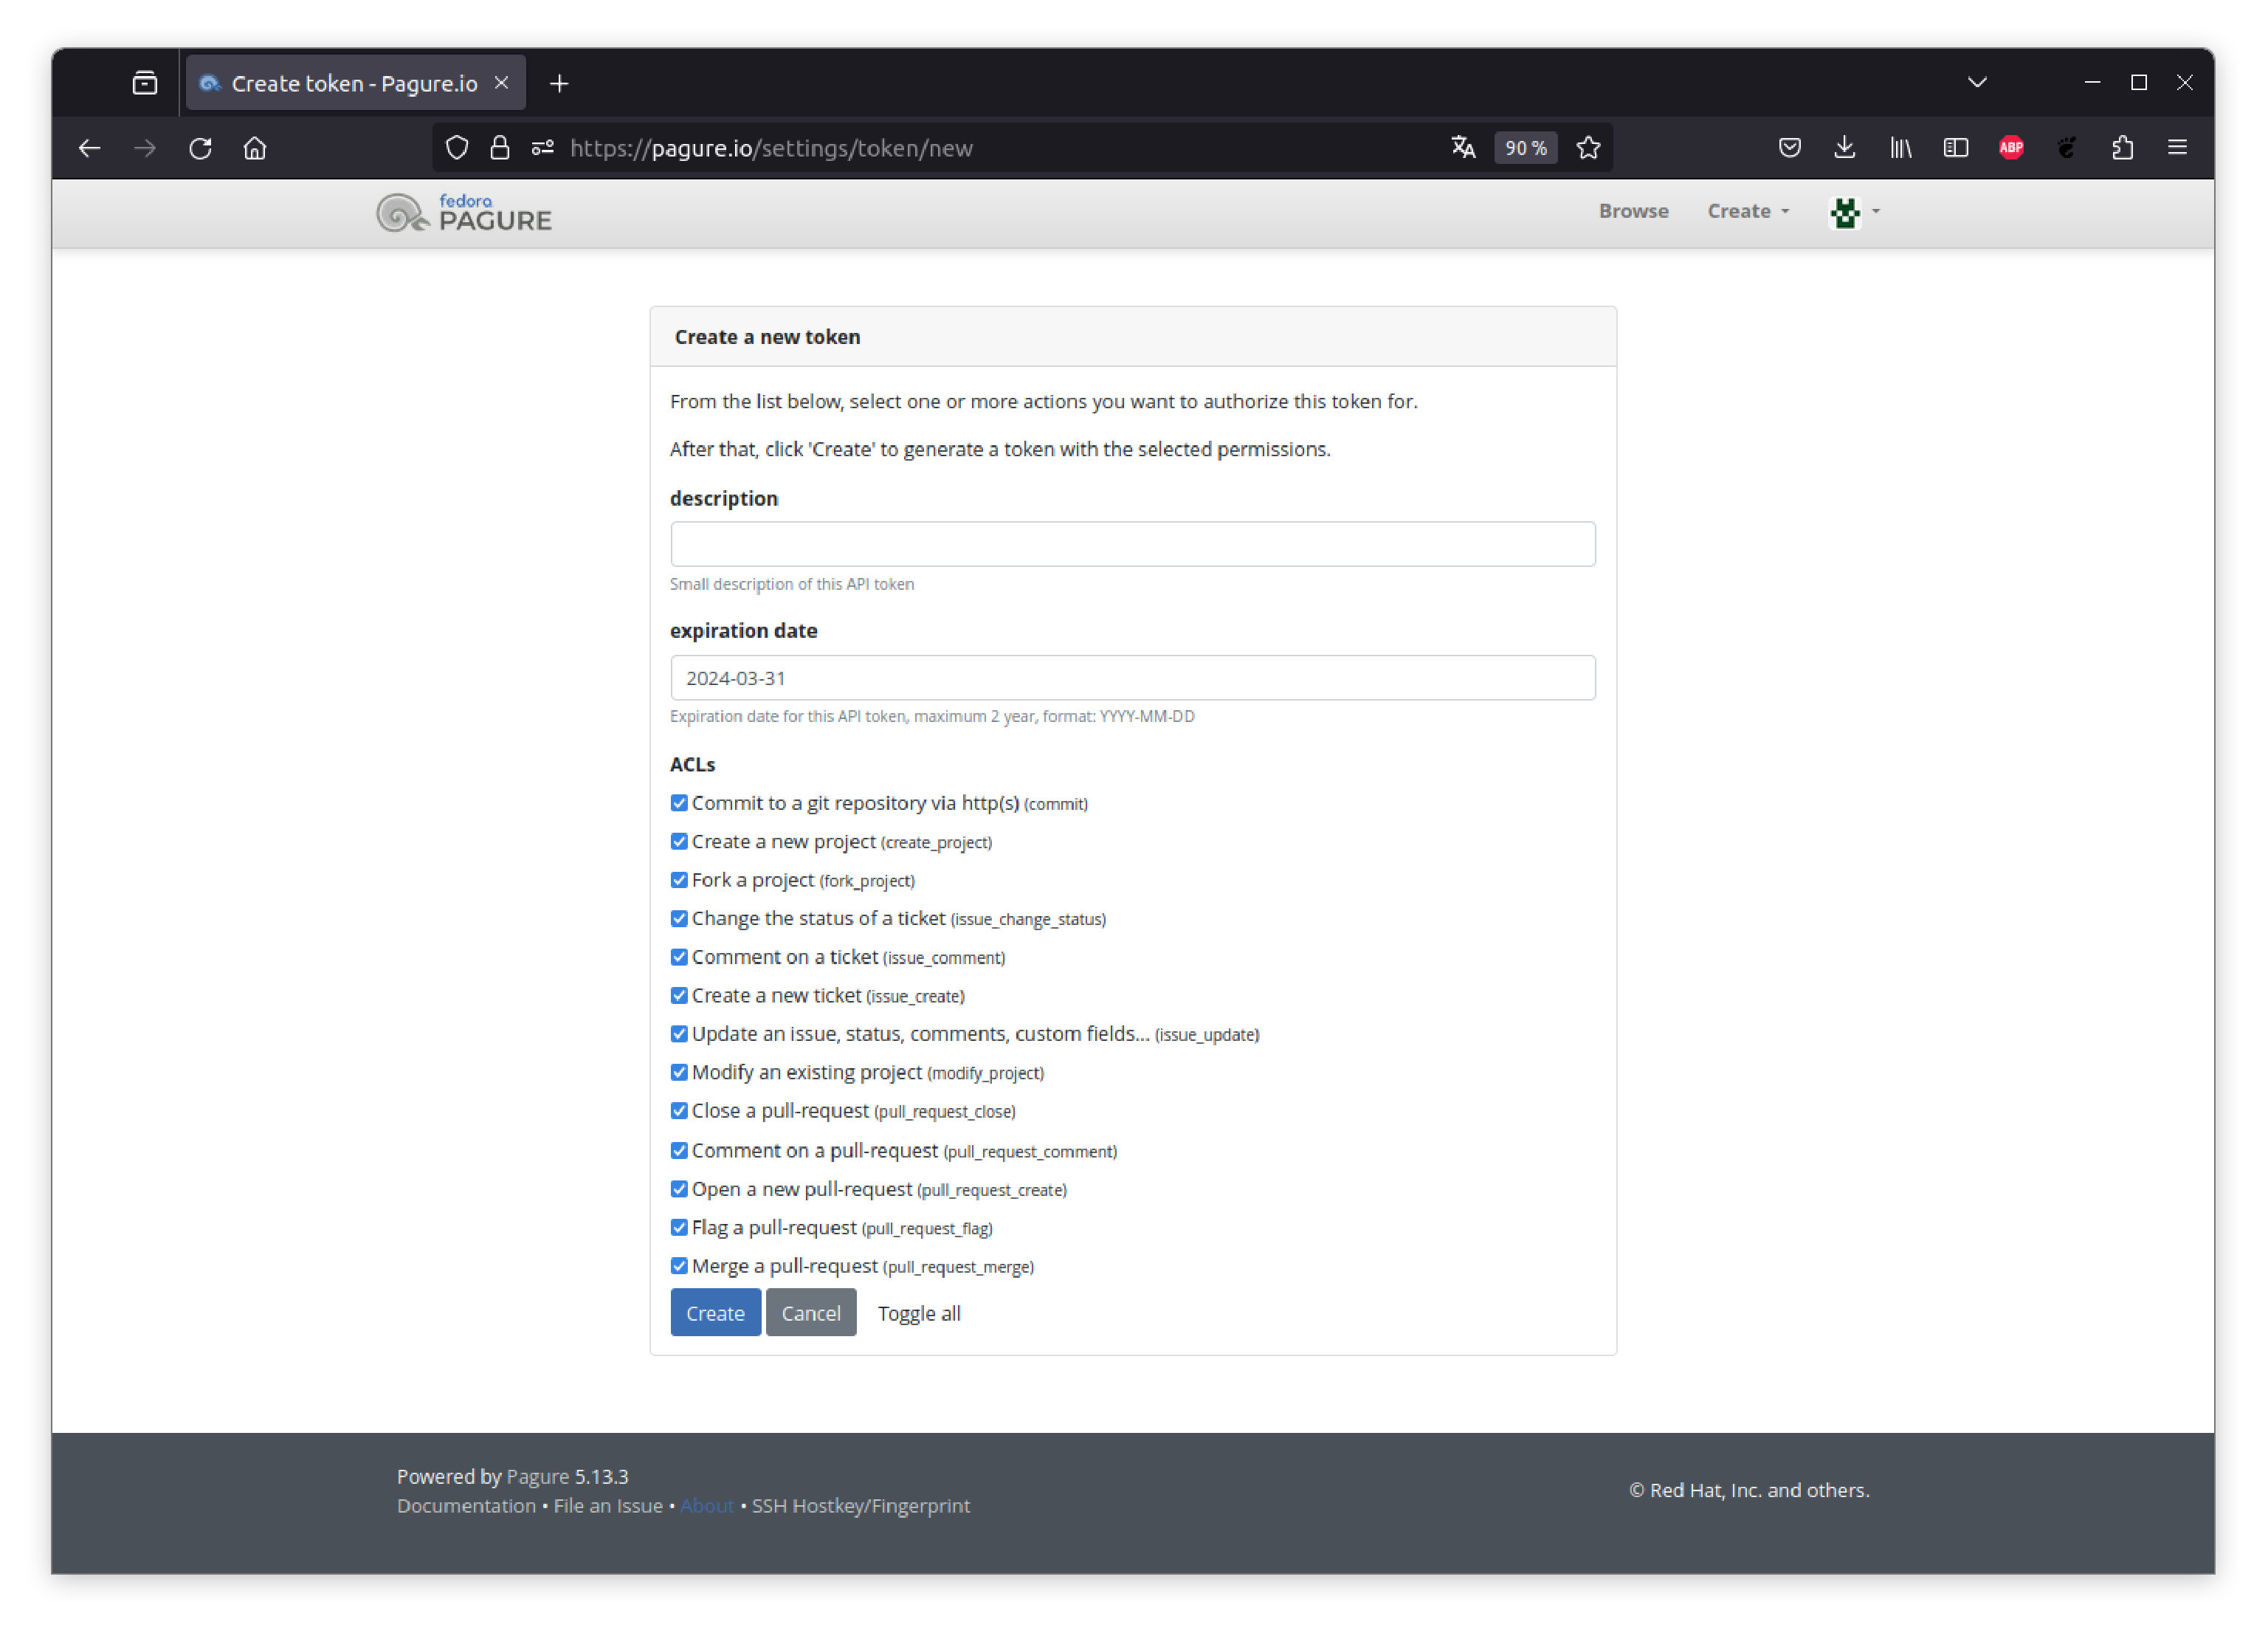
\includegraphics[width=0.75\textwidth,keepaspectratio=true,draft=\ddst]{img/rpms/pagure/pagure-1.eps}
\end{center}
You can select all available options, basically the system allows you create and work with set(s) of API Keys with different purposes. 
\item You can check the newly created API key in "\texttt{My Settings}" and then "\texttt{API Keys}"
\begin{center}
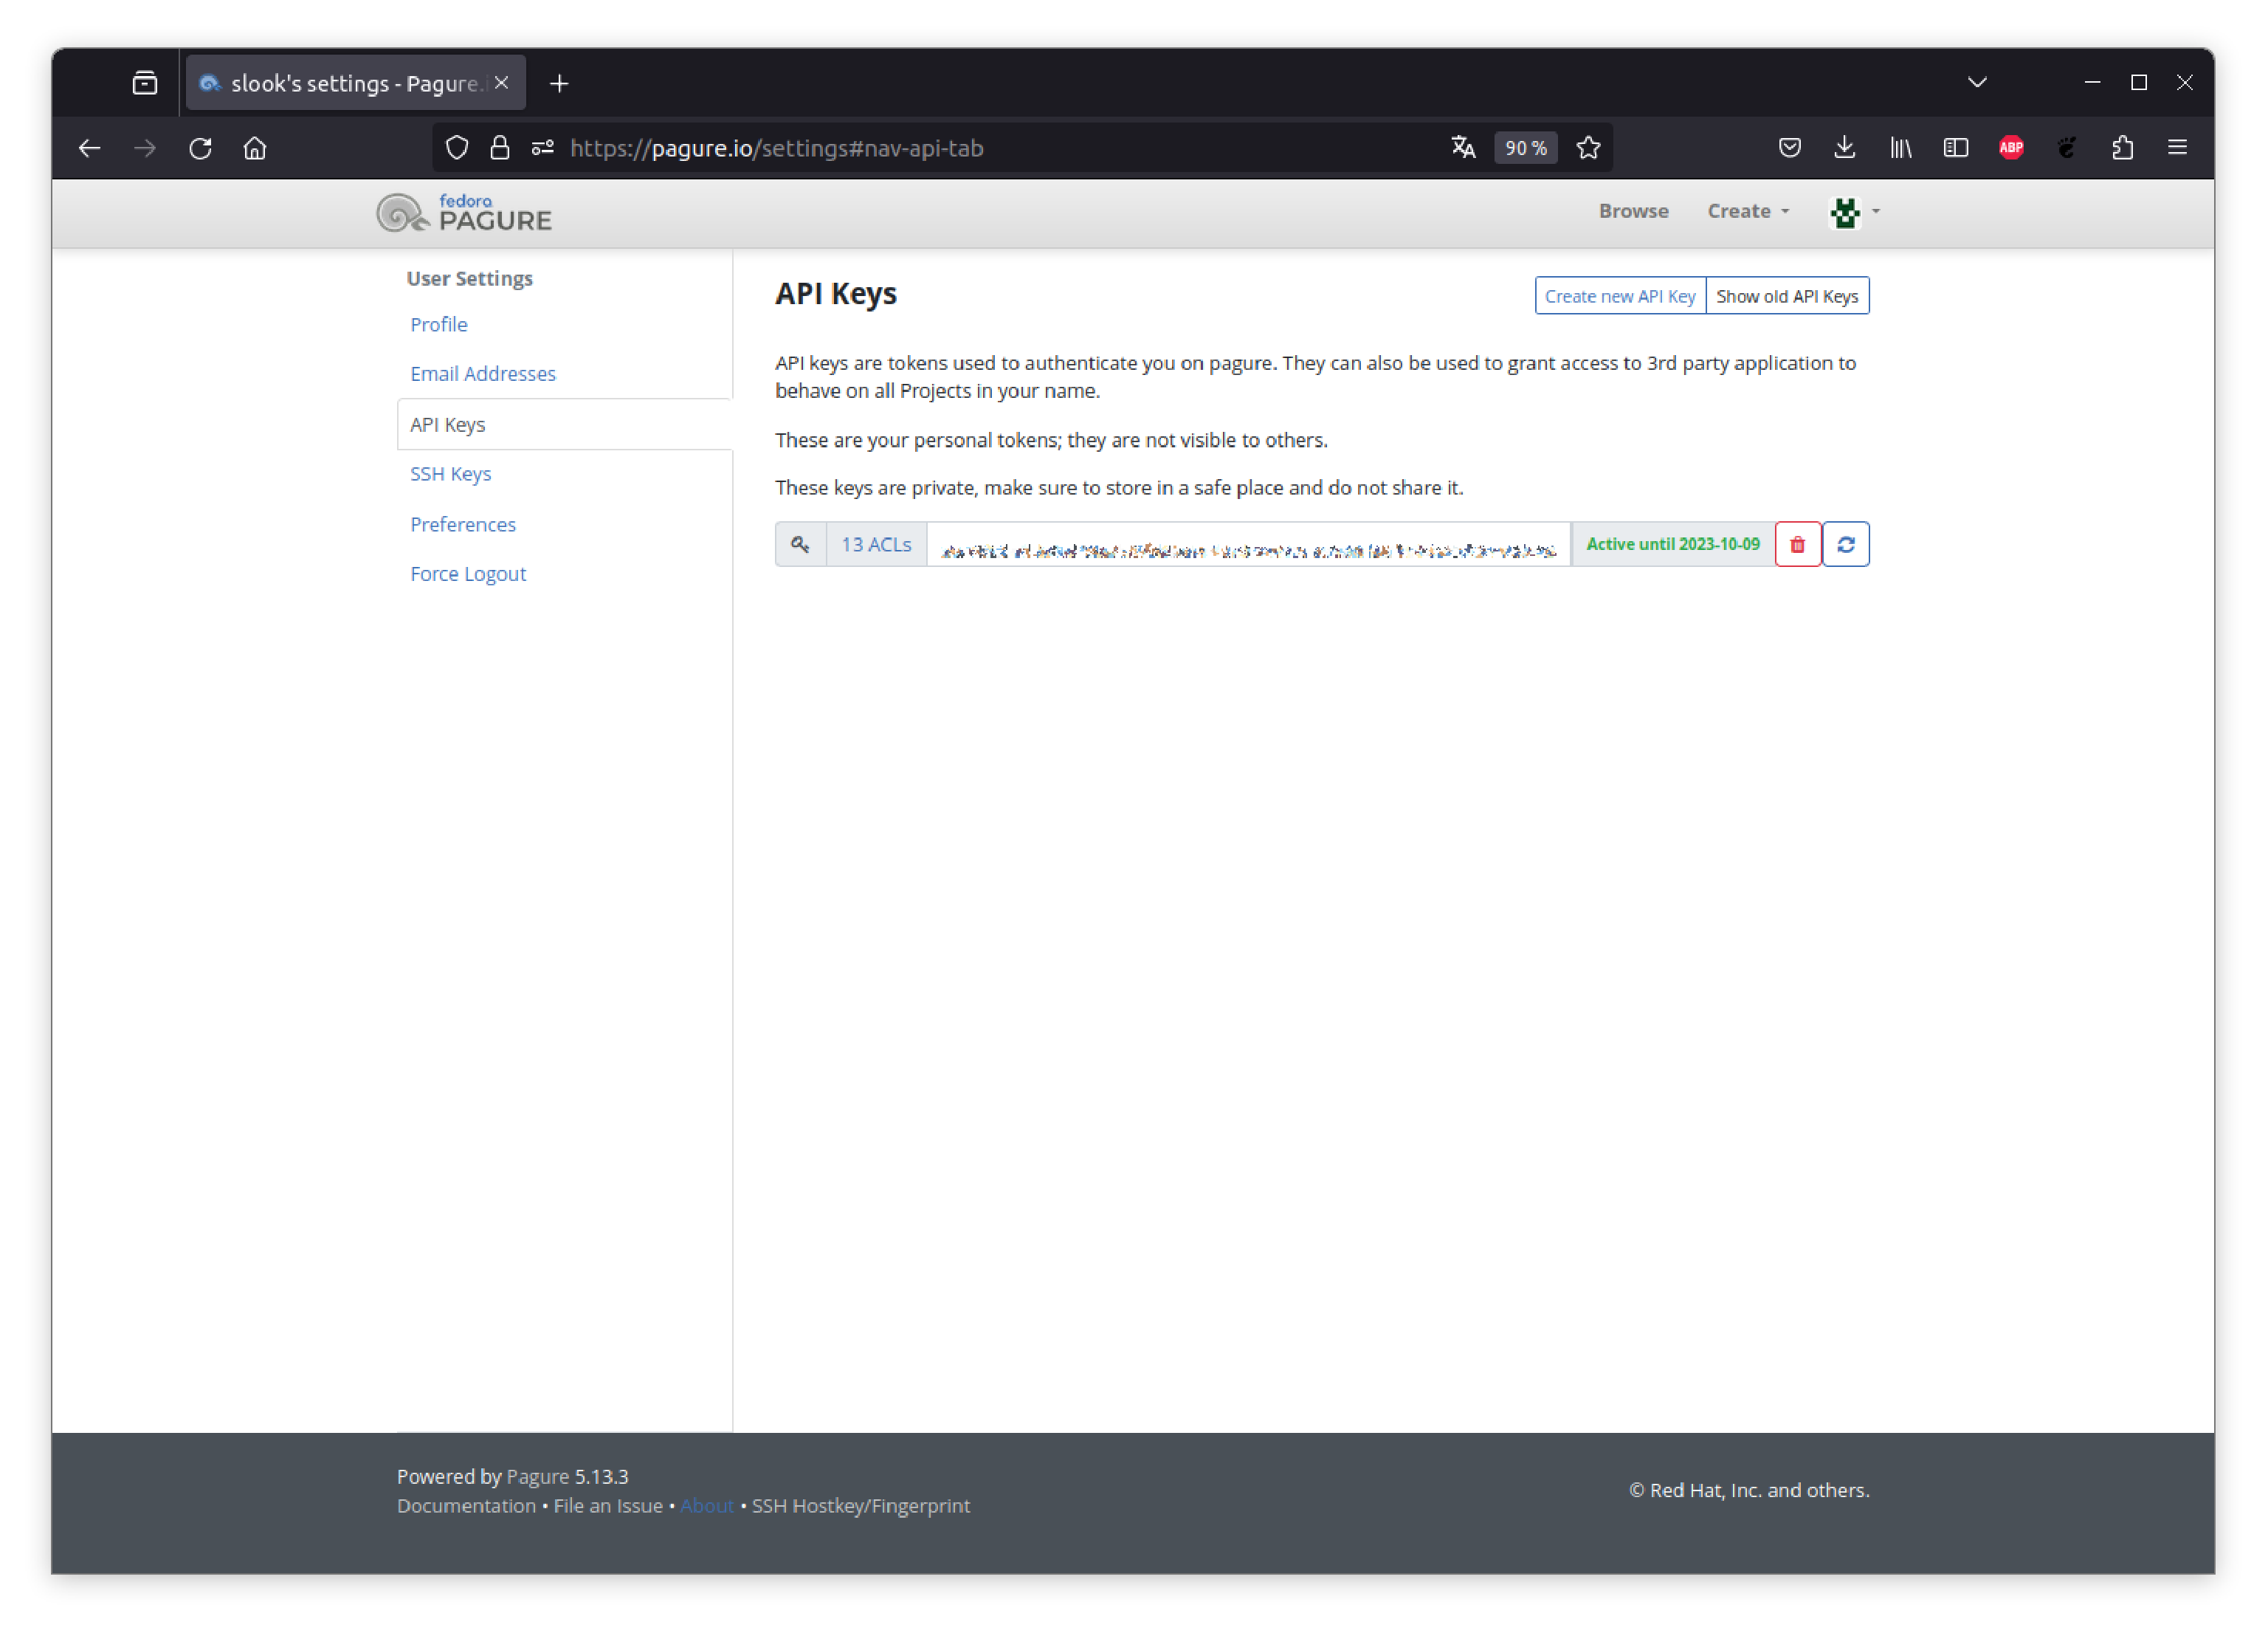
\includegraphics[width=0.75\textwidth,keepaspectratio=true,draft=\ddst]{img/rpms/pagure/pagure-3.eps}
\end{center}
\item Copy the content of the new key into: \texttt{\textasciitilde/.config/rpkg/fedpkg.conf}
\begin{scripti}
\fprompt{~} cat .config/rpkg/fedpkg.conf
[fedpkg.pagure]
url = https://pagure.io/
token = <generated-code-to-be-inserted-here>
\end{scripti}
\\[-0.75cm]
\noindent Note that the API key has an expiration date, so you will likely have to reproduce these few steps at some point in the future.
\end{enumerate}
This will ensure that the \bftt{fedpkg} command, a Fedora frontend to the \texttt{git} command, has the proper authorization access to handle the official repository of your package. 

\subsubsection{Creating the official repository for your package on \href{https://src.fedoraproject.org}{https://src.fedoraproject.org}}
\label{create_frepo}
Then it becomes possible to create the official source repository for your package. \\
The repository will be on the server \href{https://src.fedoraproject.org}{https://src.fedoraproject.org}, 
with the address:
\begin{center}https://src.fedoraproject.org/rpms/\texttt{program} \end{center}
This is where you will maintain you Fedora package, upload new source(s) and / or new package version(s). \\[0.25cm]
The repository creation is done using the \bftt{fedpkg} command:
\begin{script}
\fprompt{~} \bftt{fedpkg} \rtt{request-repo} program \dctt{???????}
\end{script}
Where: 
\begin{itemize}
\item \texttt{program} is the package name as provided in the bug message
\item \dctt{???????} is the bug message id number
\end{itemize}

\subsubsection{Uploading the package sources and / or "\texttt{.spec}" file to the official repository}

This is done using the \bftt{fedpkg} command, a Fedora frontend to the \texttt{git} command:
\begin{enumerate}
\item First, if not done already, configure your Git for Fedora packaging: 
{\small{
\begin{scripti}
\fprompt{~} \bftt{git} \rtt{config} \blue{--global} user.name "\abtt{Your Name}"
\fprompt{~} \bftt{git} \rtt{config} \blue{--global} user.email \dctt{\email}
\end{scripti}}}
\\[-0.75cm]
\item Then start by cloning the official source repository: 
\begin{scripti}
\fprompt{~} \bftt{fedpkg} \rtt{clone} prog
\end{scripti}
\\[-0.75cm]
\noindent This will copy the official Fedora source repository of "\texttt{program}" to your hard drive:
\begin{scripti}
\fprompt{~} ls prog
program.spec README.md sources
\fprompt{~}
\end{scripti}
\\[-0.75cm]
\noindent Note that you must use the name of the official Fedora repository as created in section~\ref{create_frepo}, in this case: "\texttt{program}"  
\item Download the sources from the official repository:  
\begin{scripti}
\fprompt{~} cd prog
\fprompt{~/program} \bftt{fedpkg} \rtt{sources}
\fprompt{~/program} ls
program.spec program-v1.1.tar.gz README.md sources
\fprompt{~/program}
\end{scripti}
\item Update the sources to the latest version:
\begin{scripti}
\fprompt{~/program} cp ~/program-v1.2.tar.gz .
\fprompt{~/program} \bftt{fedpkg} \rtt{new-sources} program-v1.2.tar.gz
\end{scripti}
\\[-0.75cm]
\noindent Before uploading new sources for your package to the official repository I strongly suggest that you already 
test-proofed the Koji build for this new package, see [Sec.~\ref{kojib}]. 
\item Modify the "\texttt{.spec}" file accordingly, including the \dgtt{\%changelog} section:
\begin{scripti}
\fprompt{~/program} vi program.spec 
\end{scripti}
\item Commit and push the changes:
\begin{scripti}
\fprompt{~/program} \bftt{fedpkg} \rtt{commit} \blue{-p -c}
\end{scripti}
\\[-0.75cm]
\noindent This will upload the new file(s) to: https://src.fedoraproject.org/rpms/\texttt{program}
\end{enumerate}

\subsubsection{Building the new package using the update(s)}

This is also done using the \bftt{fedpkg} command:
\begin{enumerate}
\item Request a build for Fedora branch(es), first of all for the rawhide branch:
{\small{
\begin{scripti}
\fprompt{~/program} \bftt{fedpkg} \rtt{request-branch} \blue{--repo} program \dgtt{rawhide}
\end{scripti}}}
\\[-0.5cm]
\noindent The rawhide branch is the development version of Fedora, usually the latest released version + 1. 
If the latest released is version 39 (f39), then rawhide will released as f40, 
then new rawhide branch will be created and later released as f41, and so on. \\[0.25cm]
To request a build for another Fedora branch, for instance the Fedora 39 branch, use:
{\small{
\begin{scripti}
\fprompt{~/program} \bftt{fedpkg} \rtt{request-branch} \blue{--repo} program \dgtt{f39}
\end{scripti}}}
\item To build the rawhide branch:
\begin{scripti}
\fprompt{~/program} \bftt{fedpkg} \rtt{switch-branch} \dgtt{rawhide}
\fprompt{~/program} \bftt{fedpkg} \rtt{build} \blue{--nowait}
\end{scripti}
To build the Fedora 39 branch: 
\begin{scripti}
\fprompt{~/program} \bftt{fedpkg} \rtt{switch-branch} \dgtt{f39}
\fprompt{~/program} \bftt{git} \rtt{merge} \blue{rawhide}:\dgtt{f39}
\fprompt{~/program} \bftt{git} \rtt{push} origin \blue{rawhide}:\dgtt{f39}
\fprompt{~/program} \bftt{fedpkg} \rtt{build} \blue{--nowait}
\end{scripti}
\\[-0.5cm]
\noindent For any other branch simply replace the \dgtt{f39} by the appropriate version number.
\end{enumerate}
At this stage you simply need to wait, the package will be built on Koji for the requested branches. 
If successful the builds will be available shortly to update the versions of the package in the Fedora software repository using the \href{https://bodhi.fedoraproject.org}{Bodhi} website.

\newpage
\subsubsection{Requesting for the new build(s) to update the package in the official repositories}

This is done via the web interface called Bodhi: \href{https://bodhi.fedoraproject.org}{https://bodhi.fedoraproject.org}. \\ 
\href{https://fedoraproject.org/wiki/Bodhi}{Bodhi} is a web-based system that facilitates the process of publishing package updates for Fedora. \\
\begin{center}
%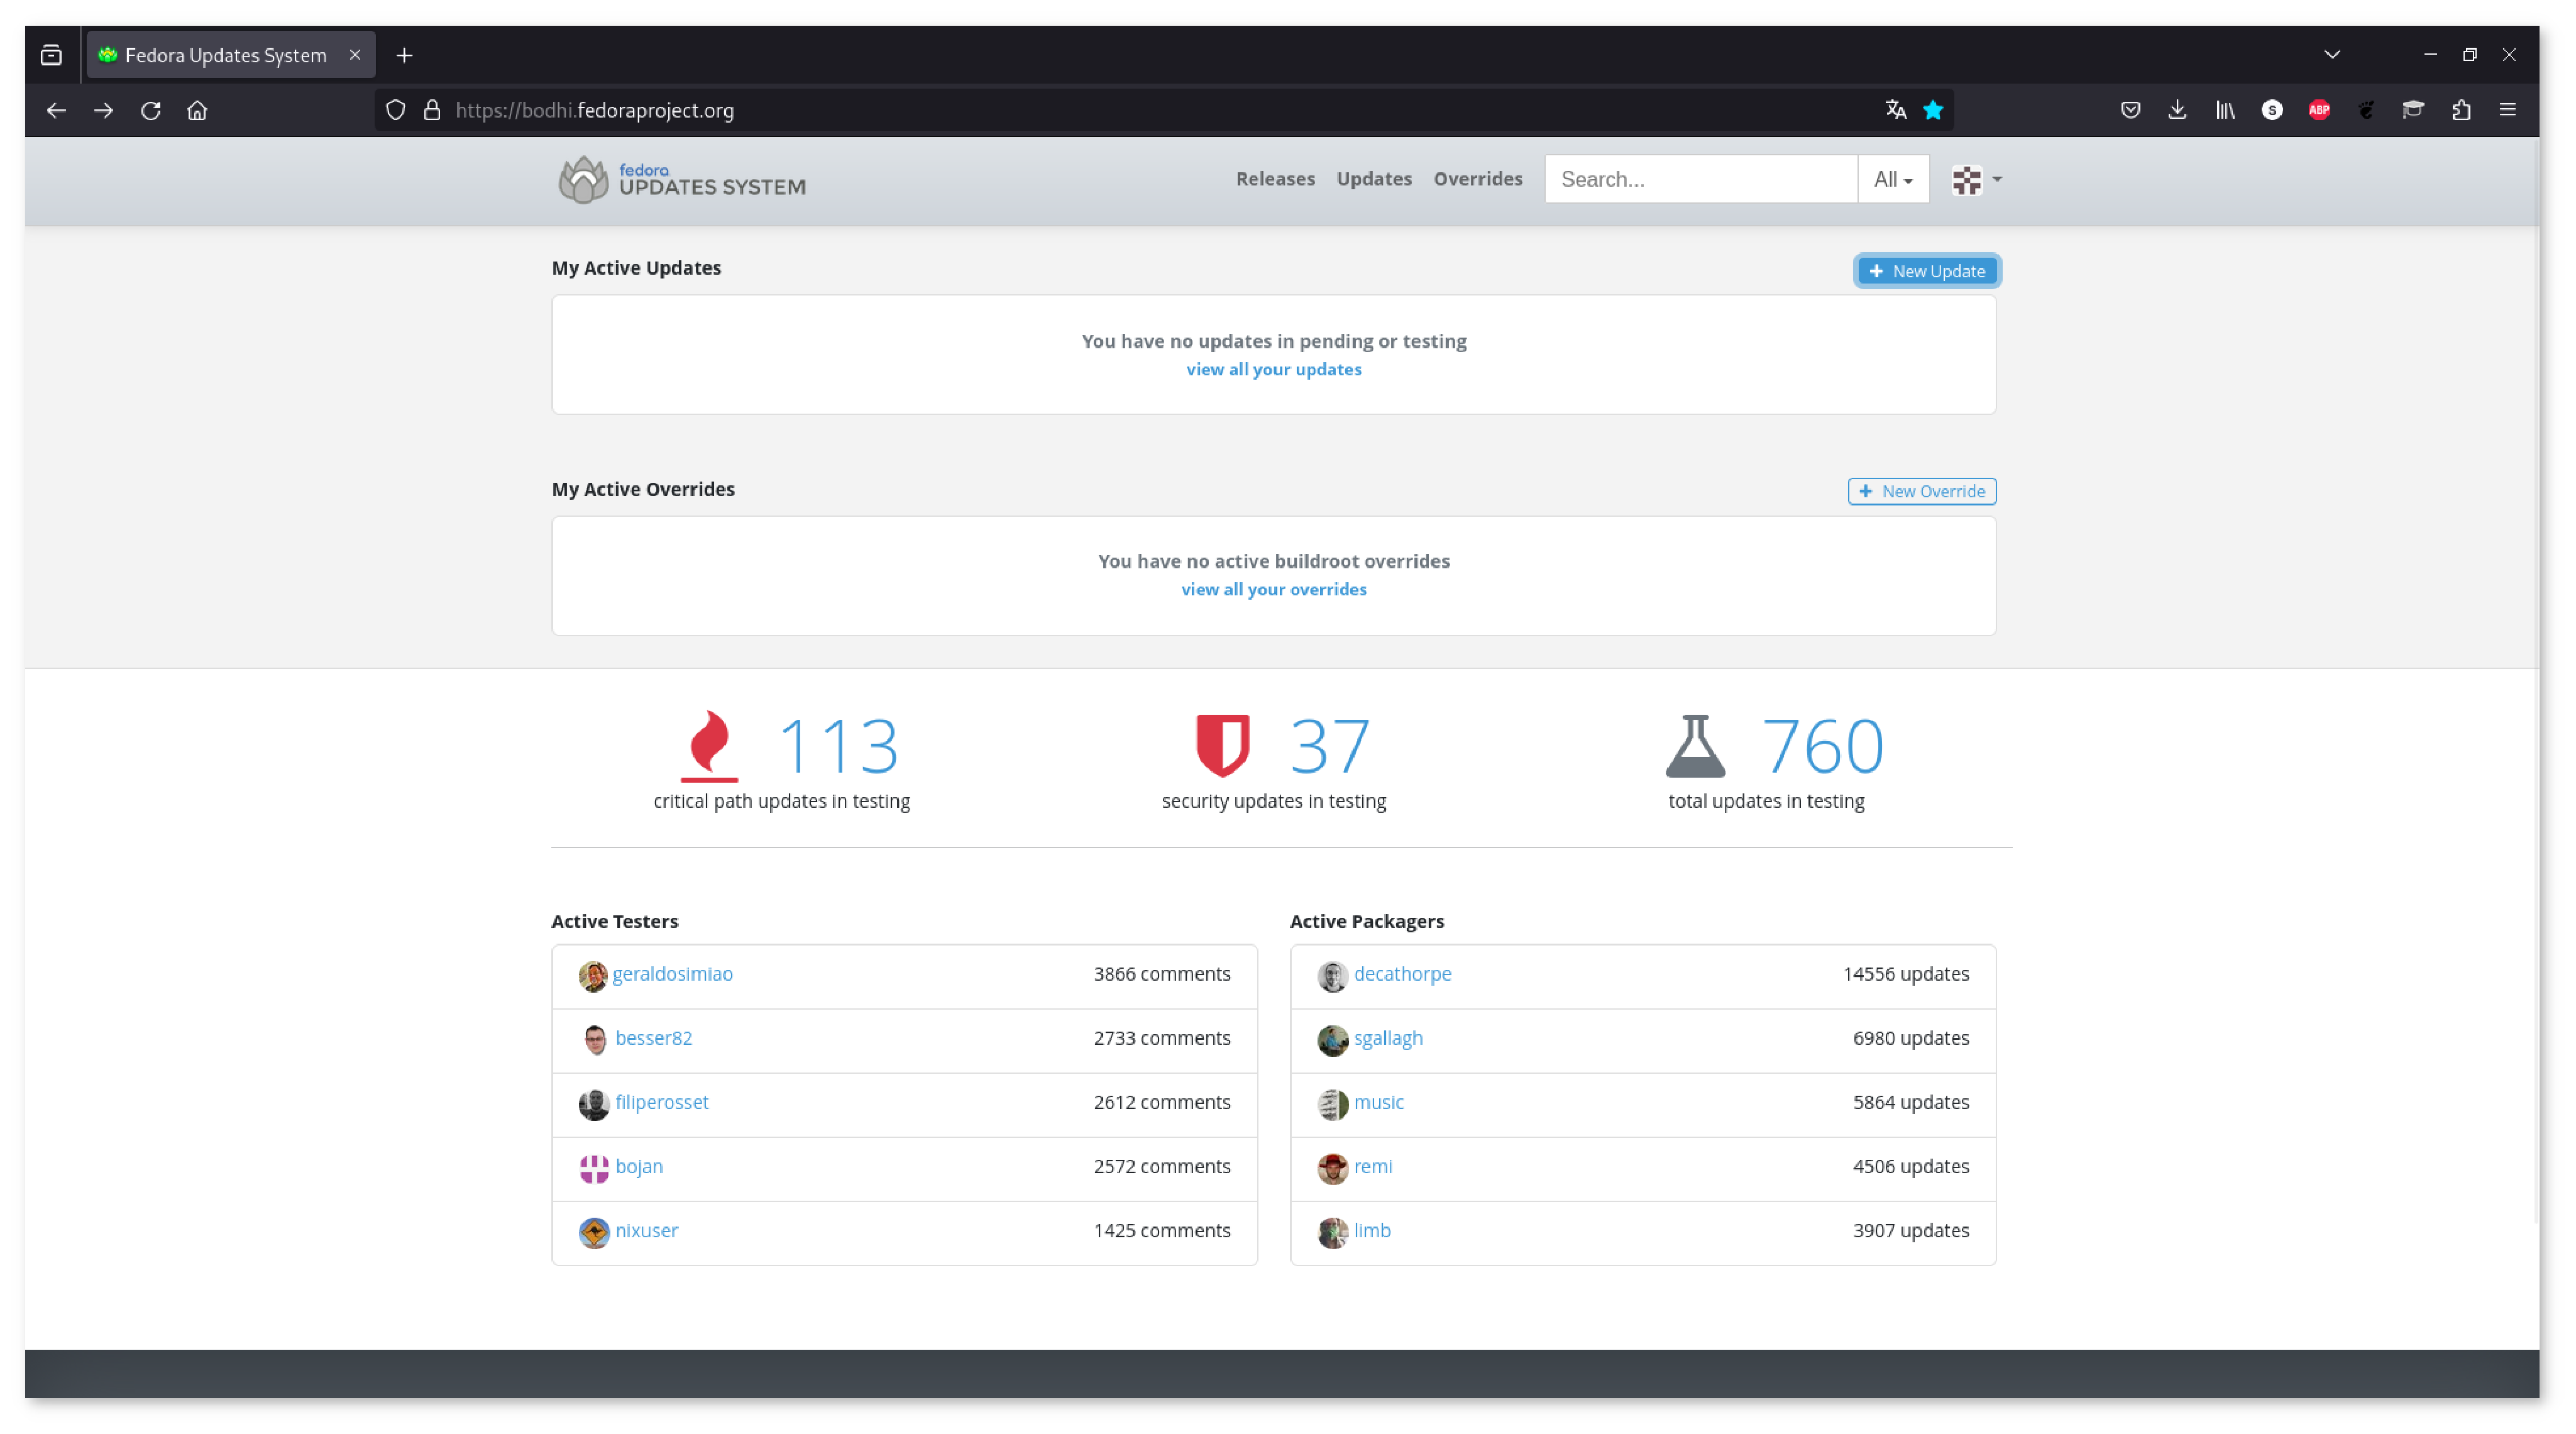
\includegraphics[width=0.75\textwidth,keepaspectratio=true,draft=\ddst]{img/rpms/bodhi/bodhi-0.eps}
\end{center}
To update the Fedora repositories with the new builds:
\begin{enumerate}
\item Login on Bodhi using your Fedora Account
\item Click on "\texttt{Updates}" 
\item Search for your package name, here "\texttt{program}" 
\item Need to create a new update to see what's next with more details
\end{enumerate}

\clearpage

\section{DEB}

\newcommand{\ddir}{"\bftt{debian}" directory}
\newcommand{\dpkg}{"\bftt{dpkg}" command}

The next pages will focus on building a DEB ("\texttt{.deb}") file suitable for distribution by \href{https://www.debian.org}{Debian} Linux. \\[0.25cm]
Maybe more importantly I will assume that you are working on Debian Linux, that would make
a lot of sense since we are talking about building Debian DEBs here. Some of the commands
I will use thereafter can only be found on Debian based Linux, therefore I would recommend to download
and install the latest Debian version either on your computer or in a virtual machine. \\[0.25cm]
To prepare a DEB file you need first to install the appropriate tools:
{\small{
\begin{script}
\uprompt{~} sudo apt install build-essential dh-make devscripts 
\uprompt{~} sudo apt install debhelper sbuild schroot debootstrap
\uprompt{~} sudo apt install debmake debmake-doc reportbug 
\uprompt{~} sudo apt install piuparts piuparts-master piuparts-slave
\end{script}
}}
\\[-0.25cm]
\noindent \bftt{dpkg} (for \bftt{D}ebian \bftt{p}ac\bftt{k}a\bftt{g}e) is the tool managing package distribution on Debian based Linux distributions. 
If I intend to provide tips and trick to help you prepare your DEB, I strongly recommend that you give a look to:
\begin{itemize}
\item \href{https://wiki.debian.org/Packaging/Intro?action=show\&redirect=IntroDebianPackaging}{Introduction to Debian Packaging}
\item \href{https://wiki.debian.org/HowToPackageForDebian}{How to package for Debian}
\item \href{https://www.debian.org/doc/debian-policy/}{Debian policy}
\item \href{https://www.debian.org/doc/manuals/packaging-tutorial/packaging-tutorial.fr.pdf}{Tutoriel: la construction de paquets Debian}
\item \href{https://wiki.debian.org/SimplePackagingTutorial}{Simple packaging tutorial}
\item \href{file://usr/share/doc/debmake-doc/}{debmake documentation}
\item \href{https://wiki.debian.org/PackagingWithGit/}{https://wiki.debian.org/PackagingWithGit/}
\end{itemize}
Indeed this guide is not meant to be a thorough review of DEB packaging, that is actually
much more complicated than for the simple desktop application used afterward to illustrate the process.

\newpage
\subsection{Prerequisites}
\label{dprereq}
We will briefly introduce hereafter the basics of Debian package construction. \\
Before starting few considerations are in order:
\begin{itemize}
\item It is required to setup properly some information and aliases.\\
To do that edit the "\texttt{\textasciitilde/.bashrc}" file and add the following lines:
\begin{scripti}
\comm{Debian packager identification}
\bad{export} \dctt{DEBEMAIL}\bad{=}\reg{\email}
\bad{export} \dctt{DEBFULLNAME}\bad{=}\reg{Your Name}

\comm{Improved lintian command for package verification}
\bad{alias} \dctt{lintian}\bad{=}\reg{lintian -EviIL +pedantic --color auto}
\end{scripti}
\item For Debian packaging to be successful the folder with the sources \red{\bf{\textsc{must}}} be of the form: 
\begin{scripti}name-version\end{scripti}
\\[-0.75cm]
With: 
\begin{itemize}
\item \texttt{name}: the package name, in example afterwards: "\texttt{program}"
\item \texttt{version}: the version number(s), in example afterwards: "\texttt{1.2.12}"
\end{itemize}
\vspace{-1cm}
\begin{scripti}
\uprompt{~} mkdir program-1.2.12
\uprompt{~} cd program-1.2.12
\end{scripti}
\\[-0.75cm]
\noindent And copy the sources in this directory. 
\end{itemize}
The process of preparing a Debian package for your program is called "Debianization", 
so let's go and Debianize away !

\newpage
\subsection{The \ddir}

The Debian package will be built using information in the \ddir\ that must be located with your sources:
{\footnotesize{
\begin{script}
\uprompt{~/program-1.2.12} ls -lh
-rw-r--r--.  1 user group  54K 24 mars  17:28 aclocal.m4
-rw-r--r--.  1 user group  481 24 mars  11:24 AUTHORS
drwxr-xr-x.  2 user group 4,0K 24 mars  17:28 \btt{autom4te.cache}
-rw-r--r--.  1 user group 2,8K 24 mars  11:24 ChangeLog
lrwxrwxrwx.  1 user group   32 24 mars  17:24 \gtt{compile}
lrwxrwxrwx.  1 user group   37 24 mars  17:24 \gtt{config.guess}
lrwxrwxrwx.  1 user group   35 24 mars  17:24 \gtt{config.sub}
-rwxr-xr-x.  1 user group 243K 24 mars  17:28 \gtt{configure}
drwxr-xr-x   5 user group 4,0K 19 sept. 17:20 \rtt{debian}
-rw-r--r--.  1 user group 3,6K 24 mars  11:24 configure.ac
-rw-r--r--.  1 user group  34K 24 mars  11:24 COPYING
drwxr-xr-x.  2 user group 4,0K 24 mars  11:24 \btt{data}
lrwxrwxrwx.  1 user group   32 24 mars  17:24 \gtt{depcomp}
-rw-r--r--.  1 user group  34K 24 mars  11:24 config.h.in
-rw-r--r--.  1 user group  16K 24 mars  11:24 INSTALL
lrwxrwxrwx.  1 user group   35 24 mars  17:24 \gtt{install-sh}
-rw-r--r--.  1 user group 4,0K 24 mars  17:03 Makefile.am
drwxr-xr-x.  2 user group 4,0K 24 mars  11:24 \btt{metadata}
lrwxrwxrwx.  1 user group   32 24 mars  17:24 \gtt{missing}
-rw-r--r--.  1 user group  247 24 mars  11:24 NEWS
drwxr-xr-x.  4 user group 4,0K 24 mars  11:24 \btt{pixmaps}
-rw-r--r--.  1 user group 4,8K 24 mars  11:24 README
drwxr-xr-x.  2 user group 4,0K 24 mars  11:24 \btt{src}
\end{script}
}}
\noindent You can generate a ready to use "\rtt{debian}" directory using:
{\footnotesize{
\begin{script}
\uprompt{~/program-1.2.12} \bftt{debmake}
\end{script}
}}
\\[-0.5cm]
\noindent If no \ddir\ is present then this command will create it, including sample files to work on. 
However this sample \ddir\ will contain some files likely unnecessary to build your first simple Debian package. \\[0.25cm]
I recommend to start working with the following files and directories:
{\footnotesize{
\begin{script}
\uprompt{~/program-1.2.12} ls -lh debian
-rw-r--r-- 1 user group  586 19 sept. 17:22 changelog
-rw-r--r-- 1 user group 3,2K 19 sept. 17:22 control
-rw-r--r-- 1 user group  39K 19 sept. 17:22 copyright
drwxr-xr-x 1 user group 4,0K 19 sept. 17:22 \btt{patches}
-rw-r--r-- 1 user group  137 19 sept. 17:22 program.install
-rw-r--r-- 1 user group   46 19 sept. 17:22 program-data.install
-rwxr-xr-x 1 user group  103 19 sept. 17:22 \gtt{rules}
drwxr-xr-x 2 user group 4,0K 19 sept. 17:22 \btt{source}
drwxr-xr-x 2 user group 4,0K 19 sept. 17:22 \btt{upstream}
-rw-r--r-- 1 user group  183 19 sept. 17:22 watch
\end{script}
}}
\\
\noindent Note that the files "\texttt{program.install}" and "\texttt{program-data.install}" are not created by the \bftt{debmake} command.  
%\begin{itemize}
%\item \bftt{patches}
%{\footnotesize{
%\begin{scripti}
%\uprompt{~/program-1.2.12} ls -lh debian/patches
%
%\end{scripti}
%}}
%\item \bftt{source}
%{\footnotesize{
%\begin{scripti}
%\uprompt{~/program-1.2.12} ls -lh debian/source
%
%\end{scripti}
%}}
%\item \bftt{upstream}
%{\footnotesize{
%\begin{scripti}
%\uprompt{~/program-1.2.12} ls -lh debian/upstream
%
%\end{scripti}
%}}
%\end{itemize}
\subsubsection{The "\texttt{changelog}" file}

The "\texttt{changelog}" file is to be updated for each new release of the program or the package, 
it describes briefly the changes in the new version:
\begin{script}
\uprompt{~/program-1.2.12} cat debian/changelog
program (1.2.12-2) unstable; urgency=medium

  * New package version

 -- Your Name <\email>  Tue, 19 Sep 2023 15:45:00 +0200

program (1.2.12-1) unstable; urgency=medium

  * Bug corrections and improvements.
  * See: \gitprog/releases/tag/v1.2.12

 -- Your Name <\email>  Mon, 17 Jul 2023 17:26:00 +0200
\end{script}

\subsubsection{The "\texttt{control}" file}

The "\texttt{control}" file contains build and runtime dependencies for your program. \\
To prepare this file requires to find the appropriate package name for each dependencies of your program: 
\begin{itemize}
\item For building the program: in the section "\texttt{Build-Depends}"
\item For running the program: in the section(s) "\texttt{Depends}" 
\end{itemize}
Dependencies are presented using coma separated lists, parenthesis can be used for specific requirement. \\
Note that the following example illustrates a "\texttt{control}" file with 2 "\texttt{Package:}" instructions, therefore 2 packages will be created:
\begin{itemize}
\item A package, architecture dependent, for the binary: "\texttt{Package: program}"
\item A package for all non-architecture dependent data: "\texttt{Package: program-data}" 
\end{itemize}
This is a standard way of doing things in the Debian world. \\
{\footnotesize{
\begin{script}
\uprompt{~/program-1.2.12} vi debian/control
\bad{Source:} program
\bad{Section:} science
\bad{Priority:} optional
\bad{Maintainer:} \var{Your Name <\email>}
\bad{Uploaders:} \var{Your Name <\email>}
\bad{Build-Depends:} debhelper-compat (= 13),
                  automake,
                  autoconf,
                  pkg-config,
                  gfortran,
                  libgfortran5,
                  libgtk-3-dev,
                  libxml2-dev,
                  libpango1.0-dev,
                  libglu1-mesa-dev,
                  libepoxy-dev,
                  libavutil-dev,
                  libavcodec-dev,
                  libavformat-dev,
                  libswscale-dev,
                  desktop-file-utils,
                  appstream-util
\bad{Standards-Version:} 4.6.2
\bad{Homepage:} \var{https://www.prog.com}
\bad{Vcs-Browser:} \var{\gitprog}
\bad{Vcs-Git:} \var{\gitprog.git}
\bad{Rules-Requires-Root:} no

\bad{Package:} program
\bad{Architecture:} any
	\bad{Depends:} program-data (= \var{\$\{source:Version\}}),
          \var{\$\{shlibs:Depends\}}, \var{\$\{misc:Depends\}},
          libgtk-3-0,
          libglu1-mesa,
          bash-completion
\bad{Description:} program is doing something
 Program is a tool box to analyze many things
 This package provides the binaries.

\bad{Package:} program-data
\bad{Architecture:} all
\bad{Multi-Arch:} foreign
\bad{Depends:} \var{\$\{misc:Depends\}}
\bad{Enhances:} program
\bad{Suggests:} program
\bad{Description:} program is doing something (data)
 Program is a tool box to analyze many things
 .
 This package contains data files for program.
\end{script}
}}\\[-0.5cm]
\noindent In the \bad{Build-Depends} section if you are CMake, or meson, replace \texttt{automake} and \texttt{autoconf} by \texttt{cmake} or \texttt{meson} respectively. 
\newpage
\noindent Few tips to help you prepare this file:
\begin{itemize}
\item The "\texttt{Section:}" keyword allows to select where the program will appear in the applications menu
\item The value for "\texttt{Standards-Version:}" changes with the Debian version:
\begin{itemize} 
\item For Debian 11: \texttt{4.5.1}
\item For Debian 12: \texttt{4.6.2}
\end{itemize}
\item The short description follows the instruction "\texttt{Description}" on the same line
\item The long description start on the next line: 
\begin{itemize}
\item Every line of the long description must start by a space character
\item Every blank line is specified using a space followed by a dot character: "\texttt{ .}"
\end{itemize}
\end{itemize}

\subsubsection{The "\texttt{copyright}" file}

The "\texttt{copyright}" file is likely the most complicated file to prepare for Debian packaging. \\
This file describes the licensing of every file in your package: 
\begin{itemize}
\item The software license for your program
\item The software license for every third-party library you ship together with the program
\item The software licence for every file in your source code with specific copyright attribution 
\end{itemize}
In each case license information must includes:
\begin{itemize}
\item The name of the software license
\item A short, if available, otherwise complete text description of the license:
\begin{itemize}
\item Every line of the license text must start by a space character
\item Every blank line in the license text is specified by a space followed by a dot: "\texttt{ .}"
\end{itemize}
\end{itemize}
The first instructions in the "\texttt{copyright}" file are providing contact information, afterwards the "\texttt{copyright}" file is organized as follow, 
with a section listing the files and the associated license:
\begin{script}
\bad{Files:}     file(s) name(s) 
\bad{Copyright:} year(s) copyright owner
\bad{License:}   License-Keyword
\end{script}
Follow later on by the associated license text information:
\begin{script}
\bad{License:} License-Keyword
 Text of the license
\end{script}
\noindent \texttt{License-keyword} information, should use the SPDX identifier: \href{https://spdx.org/licenses/}{https://spdx.org/licenses/} \\[0.5cm]
\noindent Example: 
{\footnotesize{
\begin{script}
\uprompt{~/program-1.2.12} vi debian/copyright
\bad{Format:} https://www.debian.org/doc/packaging-manuals/copyright-format/1.0/
\bad{Upstream-Name:} \var{program}
\bad{Upstream-Contact:} \var{\email}
                     \var{Your Name <\email>}
\bad{Source:} \var{\gitprog/}

\bad{Files:}      *
\bad{Copyright:} 2023-2024 Your Name
\bad{License:}   \bftt{AGPL-3.0-or-later}

\bad{Files:}      Makefile.in
             src/Makefile.in
\bad{Copyright:} 1994-2021 Free Software Foundation, Inc.
\bad{License:}   \bftt{FSFULLR}

\bad{Files:}      aclocal.m4
\bad{Copyright:} 1996-2020 Free Software Foundation, Inc.
             2004 Scott James Remnant <scott@netsplit.com>.
             2012-2015 Dan Nicholson <dbn.lists@gmail.com>
\bad{License:}   \bftt{FSFULLR} and \bftt{GPL-2.0-or-later}
\end{script}
}}
\noindent ... All other files with a license in your package must be listed as well ...
{\footnotesize{
\begin{script}
\bad{Files:}      metadata/com.program.www.appdata.xml
\bad{Copyright:} 2023-2024 Your Name
\bad{License:}   \bftt{FSFAP}

\bad{Files:}      debian/*
\bad{Copyright:} 2023-2024 your Name
\bad{License:}   \bftt{AGPL-3.0-or-later}
\end{script}
}}
\noindent ... Then all license texts are to be inserted after the file list: 
{\footnotesize{
\begin{script}
\bad{License:} \bftt{AGPL-3.0-or-later}
 Text of the AGPL v3.0 or later

\bad{License:} \bftt{FSFULLR}
 Text of the FSULLR

\bad{License:} \bftt{GPL-2.0-or-later}
 Text of the GPL v2.0 or later
\end{script}
}}
A complete example is provided in appendix~\ref{acopy}. 
\newpage
\noindent Note that some tools can be used to help you out in preparing the "\texttt{copyright}" file:
\begin{itemize}
\item \bftt{licensecheck} is command line tool to search licensed file(s) in your sources:
{\footnotesize{
\begin{scripti}
\uprompt{~/program-1.2.12} \bftt{licensecheck} \rtt{-r --copyright} \btt{.}
\end{scripti}
}}
\\[-1.5cm]
\item \bftt{scan-copyrights} helps you create a "\texttt{copyright}" file from scratch:
{\footnotesize{
\begin{scripti}
\uprompt{~/program-1.2.12} \bftt{scan-copyrights}
\end{scripti}
}}
\end{itemize}

\subsubsection{The "\texttt{patches}" directory}

This optional directory contains patch instructions required to build the Debian package, if any. \\
In that case, meaning if source patches are required then the "\texttt{patches}" directory should contain
\begin{itemize}
\item A raw text file named "\texttt{series}" containing the list of all patches to apply. 
\item As many "\texttt{.patch}" files as described in "\texttt{series}", example:
{\footnotesize{
\begin{scripti}
\uprompt{~/program-1.2.12} ls debian/patches
file-1.patch  file-2.patch  series
\uprompt{~/program-1.2.12}
\end{scripti}
}}
\\[-0.5cm]
\noindent With: \\[-0.5cm]
{\footnotesize{
\begin{scripti}
\uprompt{~/program-1.2.12} cat debian/patches/series
file-1.patch
file-2.patch
\uprompt{~/program-1.2.12}
\end{scripti}
}}
\\[-0.5cm]
\noindent And patch file, ex: "\texttt{file-1.patch}", should have the format: \\[-0.5cm] 
{\footnotesize{
\begin{scripti}
\uprompt{~/program-1.2.12} vi debian/patches/file-1.patch
Description: \bftt{this patch is doing this.}  
Author: \bftt{Your Name <\email>}
Forwarded: not-needed
Last-Update: 2023-09-19

\green{--- a/src/file.c
+++ b/src/file.c}
\bbtt{@@ -214,5 +214,5 @@}
   # The next lines to print compilers and flags:
-  printf ("FC    Compiler         : \%s\textbackslash{n}", FC);
\dctt{+  /*printf ("FC    Compiler         : \%s\textbackslash{n}", FC);}
   printf ("FC    Compiler flags   : \%s\textbackslash{n}", FCFLAGS);
   printf ("C     Compiler         : \%s\textbackslash{n}", CC);
-  printf ("C     Compiler flags   : \%s\textbackslash{n}", CFLAGS);
\dctt{+  printf ("C     Compiler flags   : \%s\textbackslash{n}", CFLAGS);*/}
\end{scripti}
}}
\\[-0.75cm] This patch will comment the lines that display compiler flags: when building the package path information is added to the compiler flags 
and you do no want that information to appear in the binary. 
\end{itemize}
To create a patch file use the "\texttt{diff}" command:
{\footnotesize{
\begin{scripti}
\uprompt{~/program-1.2.12} \bftt{diff} \rtt{-u} file.old file.new \bad{>} file.patch
\end{scripti}
}}

\subsubsection{The "\texttt{program.install}" file}

The "\texttt{program.install}" file lists the locations in the system directory tree where files are going to be installed. 
The content of this file depends on the installation process described using in your building system, for the examples listed 
in this manual: 
\begin{script}
\uprompt{~/program-1.2.12} cat debian/program.install
usr/bin
usr/share/applications
usr/share/doc
usr/share/man
usr/share/metainfo
usr/share/mime
usr/share/pixmaps
\end{script}
\noindent For the examples in this manual: \\[0.25cm]
\begin{tabular}{lp{0.25cm}lp{0.25cm}l}
\texttt{usr/bin} & & Executable & & \texttt{prog}\\
\texttt{usr/share/applications} & & Desktop entry & & \texttt{program.desktop} \\
\texttt{usr/share/doc} & & Documentation & & \texttt{README.md} \\
& & & & \texttt{AUTHORS} \\
& & & & \texttt{ChangeLog} \\
\texttt{usr/share/man} & & Manual pages & & \texttt{man1/program.1.gz} \\
\texttt{usr/share/metainfo} & & AppStream metadata & & \texttt{com.program.www.appdata.xml} \\
\texttt{usr/share/mime} & & File association(s) & & \texttt{package/program-mime.xml} \\
\texttt{usr/share/pixmaps} & & Icons and images & & \texttt{program.svg} \\
& & & & \texttt{program-project.svg} \\
& & & & \texttt{program-workspace.svg} \\
\end{tabular}
\noindent You can also have other "\texttt{.install}" file(s):
\begin{script}
\uprompt{~/program-1.2.12} cat debian/program-data.install
usr/share/program
\end{script}
The architecture non-dependent data to be installed with the program, if any.

\subsubsection{The "\texttt{rules}" file}

The \href{https://www.debian.org/doc/debian-policy/ch-source.html#main-building-script-debian-rules}{"\texttt{rules}"} file is an executable makefile 
that contains specific construction rules for your package, keep this file as simple as possible. 
Actually to package a simple application it is unlikely that you will need to modify this file at all. 
{\footnotesize{
\begin{script}
\uprompt{~/program-1.2.12} vi debian/rules
\blue{\#!/usr/bin/make -f}

\comm{Uncomment the next line to enable deb-helper verbose mode} 
\comm{export DH\_VERBOSE = 1}

\bad{export} DEB\_BUILD\_MAINT\_OPTIONS = hardening=+all

\var{\%:}
\qquad\qquad dh \var{\$@}
\end{script}
}}

\subsubsection{The "\texttt{source}" directory}

The \href{https://wiki.debian.org/debian/upstream}{"\texttt{upstream}"}  directory contains a single file: 
{\footnotesize{
\begin{script}
\uprompt{~/program-1.2.12} ls debian/sources
format
\uprompt{~/program-1.2.12} cat debian/sources/format
3.0 (quilt)
\uprompt{~/program-1.2.12}
\end{script}
}}

\subsubsection{The "\texttt{upstream}" directory}

The \href{https://wiki.debian.org/debian/upstream}{"\texttt{upstream}"} directory contains a file in YAML format describing the upstream project being packaged:
{\footnotesize{
\begin{script}
\uprompt{~/program-1.2.12} ls debian/upstream
metadata
\uprompt{~/program-1.2.12} cat debian/upstream/metadata
Bug-Database: \gitprog/issues
Bug-Submit: \gitprog/issues/new
Repository: \gitprog.git
Repository-Browse: \gitprog
Contact: \email
\uprompt{~/program-1.2.12}
\end{script}
}}

\subsubsection{The "\texttt{watch}" file}

\href{https://wiki.debian.org/debian/watch}{"\texttt{watch}"} file is used to check for newer versions of upstream software and to download it if necessary. 
For a GitHub project the syntax is as follow:
{\footnotesize{
\begin{script}
\uprompt{~/program-1.2.12} cat debian/watch
version=4

opts="filenamemangle=s\%(?:.*?)?v?(\textbackslash{d}[\textbackslash{d}.]*)\textbackslash{.}tar\textbackslash{.}gz\%program-\$1.tar.gz\%" \textbackslash
   \gitprog/tags \textbackslash
   (?:.*?/)?v?(\textbackslash{d}[\textbackslash{d}.]*)\textbackslash{.}tar\textbackslash{.}gz debian uupdate
\uprompt{~/program-1.2.12}
\end{script}
}}

\subsection{Building the "\texttt{.deb}" file(s)}

Few recommendations to build the "\texttt{.deb}" file(s): 
\begin{itemize}
\item The commands "\bftt{dh\_make}" and "\bftt{dpkg-buildpackage}" to be used to build the package are sensitive to already existing files in the upper directory, therefore before each build I recommend to clean the working directory:
{\footnotesize{
\begin{scripti}
\uprompt{~} rm -f *\_1.2.12\_*
\uprompt{~} ls
\btt{program-1.2.12}
\end{scripti}
}}
\item The commands to build the package should be run directly above the "\texttt{debian}" directory
{\footnotesize{
\begin{scripti}
\uprompt{~} cd program-1.2.12
\uprompt{~/program-1.2.12}
\end{scripti}
}}
\item The commands to build the package must be able to find a \texttt{README} file:
{\footnotesize{
\begin{scripti}
\uprompt{~/program-1.2.12} cp README.md README
\end{scripti}
}}
\end{itemize}
\newpage
\noindent Then to build the package: 
\begin{enumerate}
\item Use "\bftt{dh\_make}" to create the Debian origin tarball using the active source directory:
{\footnotesize{
\begin{scripti}
\uprompt{~/program-1.2.12} \bftt{dh\_make} \rtt{--createorig -s -y}
Maintainer Name     : Your Name
Email-Address       : \email
Date                : Thu, 02 Nov 2023 11:37:21 +0100
Package Name        : program
Version             : 1.2.12
License             : blank
Package Type        : single
You already have a debian/ subdirectory in the source tree.
dh\_make will not try to overwrite anything.
\uprompt{~} ls ../
\btt{program-1.2.12}  \rtt{program\_1.2.12.orig.tar.xz}
\end{scripti}
}}
\\[-0.75cm]
\noindent Note that this command must be performed on a clean source folder, without any object, or already compiled file(s), or any files created by the build system when preparing the software. \\ 
In the example of this manual such files could be:
\begin{itemize}
\item Compiled Fortran modules, if any "\texttt{.mod}"
\item Compiled object files "\texttt{*.o}" 
\item Autotools generated files
\end{itemize}
To avoid any issue simply remember to prepare each build using a clean source tarball.  
\item Use "\bftt{dpkg-buildpackage}" to create the package(s) using the Debian origin tarball:
{\footnotesize{
\begin{scripti}
\uprompt{~/program-1.2.12} \bftt{dpkg-buildpackage} \bad{>&} ../dpkg-build.log
\uprompt{~/program-1.2.12} ls -lh ../
total 7,0M
-rw-r--r-- 1 user group 1,1M  2 nov.  11:46 dpkg-build.log
drwxr-xr-x 7 user group 4,0K  2 nov.  11:46 \btt{program-1.2.12}
-rw-r--r-- 1 user group  16K  2 nov.  11:46 program\_1.2.12-2\_amd64.buildinfo
-rw-r--r-- 1 user group 2,2K  2 nov.  11:46 program\_1.2.12-2\_amd64.changes
-rw-r--r-- 1 user group 941K  2 nov.  11:46 \rtt{program\_1.2.12-2\_amd64.deb}
-rw-r--r-- 1 user group  14K  2 nov.  11:46 \rtt{program\_1.2.12-2.debian.tar.xz}
-rw-r--r-- 1 user group 1,3K  2 nov.  11:46 program\_1.2.12-2.dsc
-rw-r--r-- 1 user group 2,2M  2 nov.  11:45 \rtt{program\_1.2.12.orig.tar.xz}
-rw-r--r-- 1 user group 1,1M  2 nov.  11:46 \rtt{program-data\_1.2.12-2\_all.deb}
-rw-r--r-- 1 user group 1,7M  2 nov.  11:46 \rtt{program-dbgsym\_1.2.12-2\_amd64.deb}
\end{scripti}	
}}
\\[-0.5cm]
\noindent The "\bftt{dpkg-buildpackage}" builds the program and then prepare the Debian package using the result of this build. \\
Note that in the example above both results and potential errors of the commands are redirected in a log file in the top directory. \\
\end{enumerate}
After that, and if the build is successful, package(s) can then simply be installed using:
\begin{script}
\uprompt{~} \rtt{sudo} \bftt{apt} \btt{install} ./program\_1.2.12-2\_amd64.deb \textbackslash 
                                        ./program-data\_1.2.12-2\_all.deb
\end{script}
\\[-0.5cm]
\noindent It is also possible to list the content of the package using:
\begin{script}
\uprompt{~} \bftt{dpkg} \rtt{-c} ./program\_1.2.12-2\_amd64.deb
\end{script}

\subsection{Testing the "\texttt{.deb}" package and the associated files}
\label{debtesting}
After building the package, and before entering the process of having your package distributed by Debian, I strongly recommend to test it thoroughly. 

\subsubsection{lintian}
Use the "\bftt{lintian}" command to check the "\texttt{.changes}" file: 
\begin{script}
\uprompt{~} \bftt{lintian} program\_*changes 
\end{script}
\\[-0.75cm]
\noindent Note that the "\bftt{lintian}" command, that refers to the alias defined in section~\ref{dprereq}, 
is likely to produce a verbose output. \\  
If errors appear, and they likely will, some might be corrected easily while other will be more complicated to deal with. \\
In any case, all errors should be fixed in order to have the package approved as an official Debian package. 
If that is what you intent to do, then I suggest to have a list ready for the up-coming discussions with your Debian mentor during the packaging process. \\[0.25cm]
A complete local building and testing script is provided in appendix \ref{btdebs}

\subsubsection{piuparts}

You can also test the "\texttt{.deb}" files using the "\bftt{piuparts}" command:
\begin{script}
\uprompt{~} \rtt{sudo} \bftt{piuparts} ./program\_*amd64.deb 
\end{script}
\\[-0.75cm]
\noindent "\bftt{piuparts}" tests that Debian packages handle installation, upgrading, and removal correctly. 
It does this by creating a minimal Debian installation in a chroot, and installing, upgrading, and removing packages in that environment, and comparing the state of the directory tree before and after. "\bftt{piuparts}" reports any files that have been added, removed, or modified during this process. \\
Note that you need to be in the sudoers to use "\bftt{piuparts}".

\subsection{Submitting you DEB to Debian}

At this point I will consider that you already prepared you own version of the DEB package,
ideally following the guidelines provided in this manual. If not you should really take the time
to prepare a first, raw, version of your DEB. Doing so will at least tell the Debian
packagers, members of the Debian community in charge of packaging applications, that you are
willing to be part of the process, as you should. 
Ideally you should already have tested this package (see Sec.~\ref{debtesting}). \\
Also your package should meet the Debian standards, or \href{https://www.debian.org/social\_contract.html#guidelines}{Debian free software guidelines}, and requirements as listed in the \href{https://www.debian.org/doc/debian-policy/}{Debian policy manual}. \\
To submit your DEB package to the Debian community:
\begin{enumerate}
\item Create a \salsa\ account to host a version of your package.
\item Search for a suitable Debian packaging team at \href{https://wiki.debian.org/Teams}{https://wiki.debian.org/Teams}.
\item Post an ITP message on \href{http://www.debian.org/devel/wnpp/}{WNPP} Debian Official Work-Needing and Prospective Packages.
\item Create a message to introduce yourself to the Debian community and search for a mentor and sponsor to review your package.
\end{enumerate}

\subsubsection{Create a Salsa account}

\salsa\ is a collaborative development server for Debian based on the \href{https://gitlab.com}{GitLab} software. 
\salsa\ is supposed to provide the necessary tools for package maintainers, packaging teams and other Debian related individuals and groups for collaborative development (see [Fig.~\ref{salsa}]).
\begin{figure}[!h]
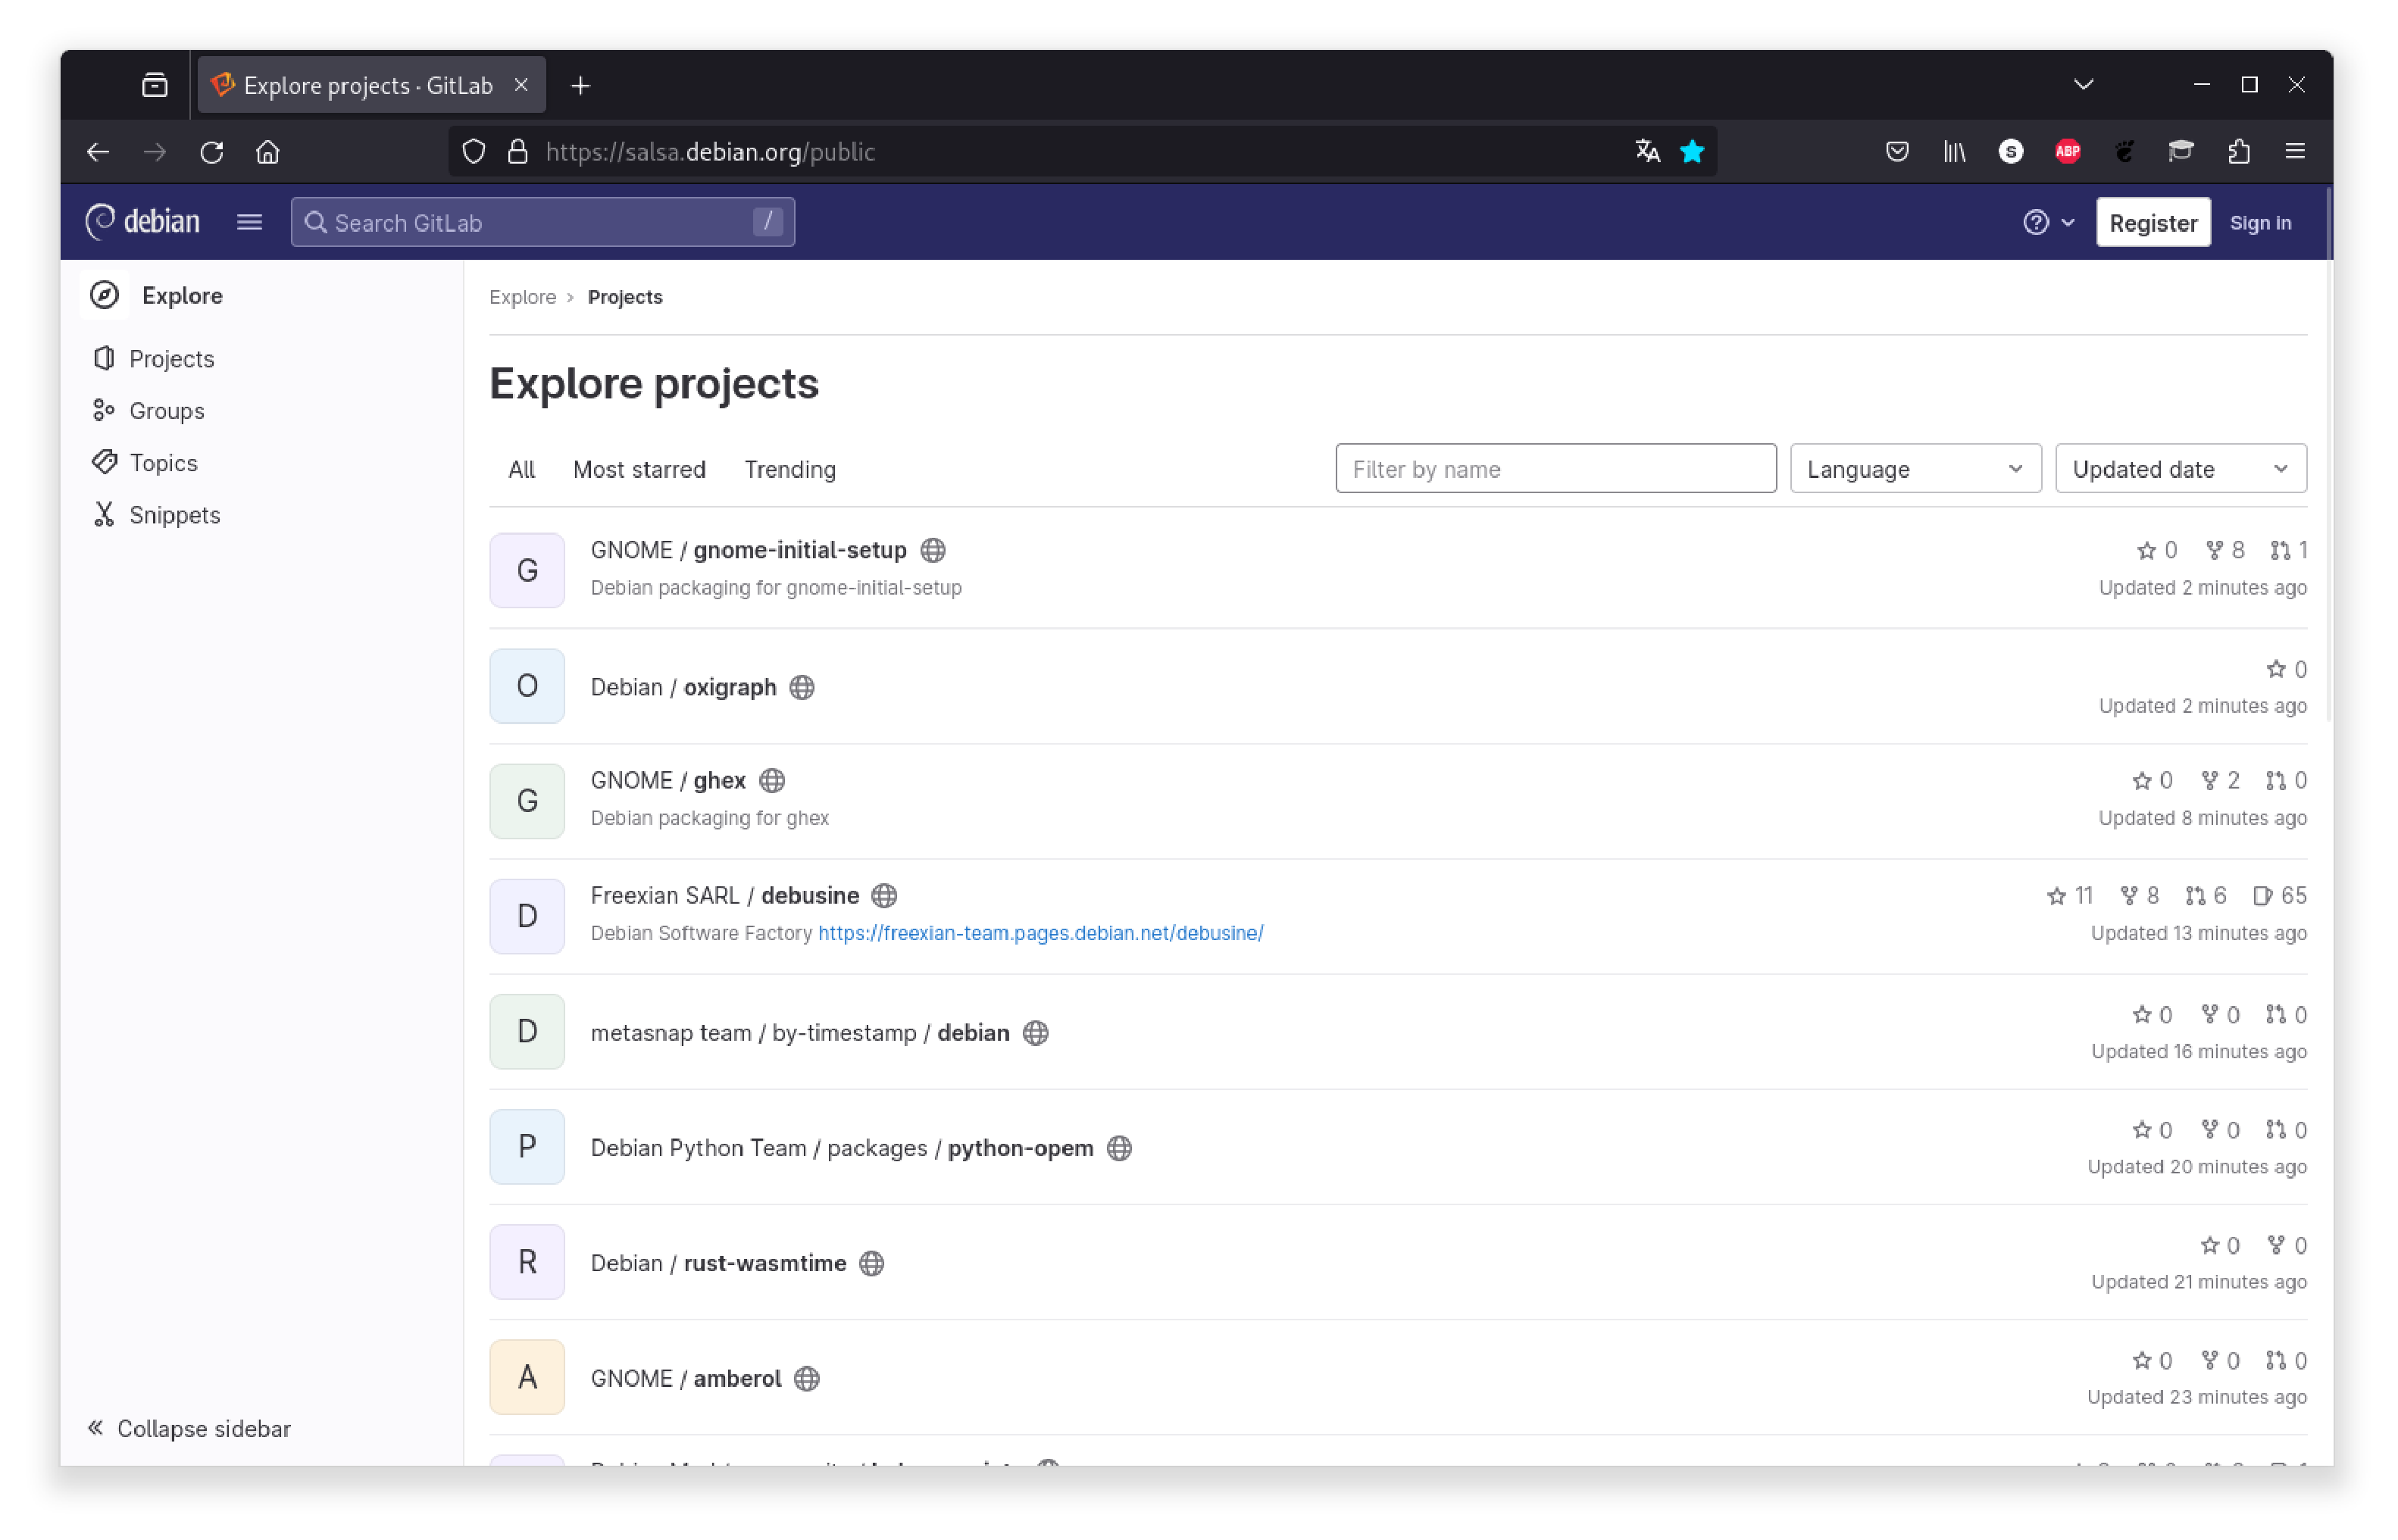
\includegraphics[width=1.0\textwidth,keepaspectratio=true,draft=\ddst]{img/deb/salsa}
\caption{The Debian \salsa\ web site}\label{salsa}
\end{figure}

\subsubsection{Search for suitable Debian packaging team}

In order to find a mentor and a sponsor to help you to get your package approved, search for suitable teams on \href{https://wiki.debian.org/Teams}{https://wiki.debian.org/Teams}. \\
In particular browse the parts dedicated to:
\begin{itemize}
\item Blends teams: \href{https://wiki.debian.org/Teams\#Blends\_teams}{https://wiki.debian.org/Teams\#Blends\_teams}
\item Packaging teams: \href{https://wiki.debian.org/Teams\#Packaging\_teams}{https://wiki.debian.org/Teams\#Packaging\_teams}
\end{itemize}
This is where you are likely to get in touch with people interested by your software. \\
For example to package "\href{https://atomes.ipcms.fr}{\bf{atomes}}" I got in touch with the \href{https://wiki.debian.org/Debichem}{Debichem} team. 

\newpage

\subsubsection{Post an ITP message that will appear on WNPP}

\href{http://www.debian.org/devel/wnpp/}{WNPP} Debian Official Work-Needing and Prospective Packages, is the official Debian website that holds, 
among other things, the list of the prospective packages for the Debian community: 
\begin{itemize}
\item Packages being worked on ({\bf{I}}ntent {\bf{T}}o {\bf{P}}ackage)
\item Requested packages ({\bf{R}}equest {\bf{F}}or {\bf{P}}ackaging)
\end{itemize}
By posting an ITP message on Debian's WNPP you are announcing that you intend to do the packaging yourself. 
If your package meets Debian standards, then you can look for a Mentor and Sponsor to review your package and upload it. \\[0.25cm]
To post the ITP message requires to use the command line and the \href{https://wiki.debian.org/reportbug}{"\texttt{reportbug}"} utility:
\begin{enumerate}
\item Prepare a complete text message that describe your package, including:
\begin{itemize}
\item Short description
\item Long description
\item Demonstration of the interest for the community
\item Request for sponsorship
\end{itemize}
A detailed example is provided in appendix \ref{bugreport}. 
\item Configure "\texttt{reportbug}":
\begin{enumerate}
\item Run "\texttt{reportbug --configure}" to create a "\texttt{\textasciitilde/.reportbugrc}" configuration file.
\item Follow the instructions and when asked: \\
"\texttt{Do you have a 'mail transport agent' (MTA) ... configured ?}" \\
choose \bftt{No}
\item Then enter the SMTP host for your mail server
\item For the user name enter your email address
\item For the question: \\
"\texttt{Does your SMTP host require TLS authentication ?}" \\
choose \bftt{Yes}
\end{enumerate}
You can edit the file "\texttt{\textasciitilde/.reportbugrc}" in particular to add your password:
{\footnotesize{
\begin{scriptii}
\uprompt{~} vi .reportbugrc
\comm{ reportbug preferences file}
\comm{ character encoding: UTF-8}
\comm{ Version of reportbug this preferences file was written by}
reportbug\_version \rtt{"7.10.3+deb11u1"}
\comm{ default operating mode: one of: novice, standard, advanced, expert}
mode novice
\comm{ default user interface}
ui text
\comm{ offline disables querying information over the network}
\comm{offline}
\comm{ name and email setting (if non-default)}
realname \rtt{"Your Name"}
email \rtt{"\email"}
\comm{ Send all outgoing mail via the following host}
smtphost \rtt{"www.webserver.eu"}
smtpuser \rtt{"\email"}
smtppasswd \rtt{"Your-Password-Here"}
\comm{ Require STARTTLS for the SMTP host connection}
smtptls
\comm{ If nothing else works, remove the \# at the beginning}
\comm{ of the following three lines:}
\comm{no-cc}
\comm{list-cc-me}
\comm{smtphost reportbug.debian.org}
\comm{ You can add other settings after this line.  See}
\comm{ /etc/reportbug.conf for a full listing of options.}
\end{scriptii}
}}
\item Use "\bftt{reportbug} \rtt{wnpp}" to send your ITP message:
{\footnotesize{
\begin{scripti}
\uprompt{~} \bftt{reportbug} \rtt{wnpp}
\end{scripti}
}}
\\[-0.75cm]
\noindent Then simply follow the prompt: 
\begin{enumerate}
\item This is an ITP
\item Enter the proposed package name: "\texttt{program}"
\item Enter the short description 
\item Press "\texttt{s}" to skip he bug message search
\item Complete and send the message, note that "\texttt{reportbug}" uses a \href{https://www.vim.org}{vi} interface:
\begin{itemize}
\item To insert text press \keystroke{i}, then input your text. \\
To navigate the document use the keyboard arrows \LArrow, \RArrow, \UArrow and \DArrow.
\item To save the message and to send it:
\begin{itemize}
\item Press \Esc
\item Press \keystroke{:}
\item Input: \\[-1cm]
\begin{scriptiii}
\texttt{x!}
\end{scriptiii}
\\[-1.5cm]
\item Press \Enter
\end{itemize}
\end{itemize}
Note that you can modify each line from the "\texttt{Subject}" first line to end of the message, 
including the package name and the short description if required.
\end{enumerate}
\end{enumerate}
When the message has been sent you will receive an email carbon copy of your message, as well as another message acknowledging your request and including a bug number as well as a link to follow the discussion on-line. \\
This message will have the following subject: 
\begin{script}
Bug#\rtt{???????}: Acknowledgment (\magenta{ITP:} \bftt{program} \magenta{--} \bftt{short description})
\end{script}
\\[-0.75cm]
\noindent where "\rtt{???????}" is the bug number associated with your ITP. \\
The link to follow the discussion on-line will be like:
\begin{script}
https://bugs.debian.org/cgi-bin/bugreport.cgi?bug=\rtt{???????}
\end{script}
\\[-0.75cm]
Now what's left is to introduce your self to the Debian packaging community. 

\subsubsection{Introduce yourself to the Debian community}

Simply send an email to the team you identify in the previous stage, to introduce your self, your work, and of course your program, also do not forget to mention the ITP bug number on WNPP. \\
Remember that Debian puts a lot of focus on quality, thus the better your package is prepared before submitting the ITP the easier it will be to find sponsorship. Sponsors might be hard to find and busy, helping them out to do the job is helping your package to be accepted more easily. \\
You can always get help from:
\begin{itemize}
\item Other members of a packaging team: \href{https://wiki.debian.org/Teams}{https://wiki.debian.org/Teams}
\item The Debian Mentors group (if your package does not fit in a team):
\begin{itemize}
\item \href{https://wiki.debian.org/DebianMentorsFaq}{https://wiki.debian.org/DebianMentorsFaq}
\item \href{http://mentors.debian.net/}{http://mentors.debian.net/}
\item The mentors mailing list: \href{mailto:debian-mentors@lists.debian.org}{debian-mentors@lists.debian.org}
\end{itemize}
\item Documentation: \href{http://mentors.debian.net/intro-maintainers}{http://mentors.debian.net/intro-maintainers}
\item Localized mailing list (in your own language) "debian-devel-\{language\}@lists.d.o":
\begin{itemize}
\item \href{mailto:debian-devel-french@lists.d.o}{debian-devel-french@lists.d.o}
\item \href{mailto:debian-devel-spanish@lists.d.o}{debian-devel-spanish@lists.d.o}
\end{itemize}
\end{itemize}

\subsubsection{After that: the next steps}

As for the RPM side, the next steps of the process are not up to you, or not entirely anyway.
As soon as both personal introduction and bug message have been sent, the community feedback
is required for your package to go further. 
Debian Mentors and Packager(s) will look into your bug message to test your package. 
The more your ensured that your package follows the official Debian packaging guidelines
the more easily your package will be accepted.
The most complicated part is likely to find a Mentor, an official Debian package maintainer
experienced enough to be allowed to register new package and their maintainer. This is done
via exchanges with the Debian packaging community, here are some advise:
\begin{itemize}
\item The process can take time: be patient !
\item Search for people that could be interested by your software in the community: remember
that a good introduction is the best starting point !
\item When you have someone to talk to, ask what to do to help: be part of the process all the
way through !
\end{itemize}

\subsection{Managing your official DEB package for Debian}

At this point I will assume that your DEB package has been approved by your mentor. \\
When done she or he, will create the official repository on \salsa. \\ 
Togheter you will have decided on the most suitable packaging team for your program. \\ 
Each teams has a group on \salsa, for example the Debichem team  
regroups chemistry related packages: \href{https://salsa.debian.org/debichem-team}{https://salsa.debian.org/debichem-team}. \\[0.25cm]
You can search for teams and the corresponding group on \salsa\ at: \\[0.25cm]
\href{https://wiki.debian.org/Teams\#Packaging\_teams}{https://wiki.debian.org/Teams\#Packaging\_teams} \\[0.25cm]
Then "Request Access" to the packaging team for your package. \\[0.25cm]
Your mentor will create a repository for your package in the selected packaging team, once the membership granted you will be able 
to upload data in your repository on \salsa\ at the address:
\begin{center}https://salsa.debian.org/PACKAGING-team/Program\end{center}
The official respository for your package on \salsa\ will contain 3 branches:
\begin{itemize}
\item "\texttt{upstream}": the sources of your program
\item "\texttt{pristine-tar}": the "\texttt{orig}" archive for your package, that contains both sources and the "\texttt{debian}" directory to build the DEB package. 
\item "\texttt{master}": the sources of your program and the "\texttt{debian}" directory to build the DEB package
\end{itemize}
Debian offers a tool to hanlde packaging using the \bftt{git} command:
\begin{script}
\uprompt{~} sudo apt install git-buildpackage
\end{script}\\[-0.5cm]
\noindent The Debian package "\texttt{git-buildpackage}" provides acces to the \bftt{gbp} command that you can use to maintain your package with Git:
\begin{itemize}
\item Upload the new sources on the \texttt{master}" branch using standard Git commands: 
\begin{scripti}
\uprompt{~/program-1.2.12} git checkout master
\uprompt{~/program-1.2.12} git add .
\uprompt{~/program-1.2.12} git commit -a
\end{scripti}
\\[-1.25cm]
\item Then use the "\bftt{gbp}" for \bftt{g}it \bftt{b}uild \bftt{p}ackage to build the package:
\begin{scripti}
\uprompt{~/program-1.2.12} \bftt{gbp} \rtt{buildpackage}
\end{scripti}
\\[-0.75cm] This will trigger the build of the source and binary packages from your Salsa repository.
\item When you have produced a release ready package, tag it using:
\begin{scripti}
\uprompt{~/program-1.2.12} \bftt{gbp} \rtt{buildpackage} \btt{--git-tag}
\end{scripti}
\\[-0.75cm]
\noindent This creates a tag, as illustrated in the chapter dedicated to hosting platforms (Sec.~\ref{gtags}), simply using Git, the tag is extracted from the file "\texttt{debian/changelog}" and will have the form: \texttt{debian/version}", where "\texttt{version}" is the last version number in the file "\texttt{debian/changelog}", in this example "\texttt{1.2.12}", 
\end{itemize}
For more information on \bftt{gbp}: \href{https://wiki.debian.org/PackagingWithGit}{https://wiki.debian.org/PackagingWithGit} \\[0.25cm]
At this point your package is almost ready to integrate the official Debian respositories, the remaining tasks are up to an official Debian developper. Contact your Debian mentor or the packaging team that accepted your software to let them know so that they can finish up the packaging process. 
\newpage

\section{Flatpak}

Flatpak is an application deployment framework for desktop applications. 

\subsection{Prerequesites}

Give a look to the following tutorials:
\begin{itemize}
\item \href{https://flatpak.org/setup}{https://flatpak.org/setup}
\item \href{https://docs.flatpak.org/en/latest/first-build.html}{https://docs.flatpak.org/en/latest/first-build.html}
\end{itemize}
To install Flatpak and the tools require to build your program use:
\begin{itemize}
\item Install Flatpak: 
\begin{itemize}
\item Fedora: 
{\footnotesize{
\begin{scriptii}
\fprompt{~} \bftt{sudo} \rtt{dnf} \btt{install} flatpak
\end{scriptii}
}}
\item Debian:
{\footnotesize{
\begin{scriptii}
\uprompt{~} \bftt{sudo} \rtt{apt} \btt{install} flatpak
\uprompt{~} \bftt{sudo} \rtt{apt} \btt{install} gnome-software-plugin-flatpak
\end{scriptii}
}}
\end{itemize}
\item Install the Flathub repository: 
{\scriptsize{
\begin{scripti}
\bftt{flatpak remote-add} \rtt{-{-}if-not-exists} \btt{flathub} https://dl.flathub.org/repo/flathub.flatpakrepo
\end{scripti}
}}
\item Install the suitable Flatpak runtime:
{\footnotesize{
\begin{scripti}
\bftt{flatpak} \rtt{install} \rtt{flathub} \btt{org.freedesktop.Platform//22.08}
\end{scripti}
}}
\item Install the corresponding Flatpak Software Development Kit 'SDK':
{\footnotesize{
\begin{scripti}
\bftt{flatpak} \rtt{install} \rtt{flathub} \btt{org.freedesktop.Sdk//22.08}
\end{scripti}
}}
\item Install the Flatpak builder:
{\footnotesize{
\begin{scripti}
\bftt{flatpak} \rtt{install} \rtt{flathub} \btt{org.flatpak.Builder}
\end{scripti}
}}
\end{itemize}

\subsection{To build the Flatpak}

\begin{enumerate}
\item Prepare the YAML file that describe your project: "\texttt{org.flatpak.prog.yml}"
\item Init a Git repository and install the shared modules repository (required to use glu)
\item Build the Flatpak
\end{enumerate}

\subsubsection{The file "\texttt{org.flatpak.prog.yml}"}

This file describes the contruction protocole to build the Flatpak for your project:
{\footnotesize{
\begin{script}
\var{app-id}: org.flatpak.prog
\var{runtime}: org.freedesktop.Platform
\var{runtime-version}: \magenta{'22.08'}
\var{sdk:} org.freedesktop.Sdk
\var{command:} prog
\var{modules:}
  - shared-modules/glu/glu-9.json
  - \var{name:} prog
    \var{buildsystem:} autotools
    \var{no-autogen:} \magenta{true}
    \var{sources:}
      - type: archive
        url: https://github.com/AUTHOR/RESPOSITORY/archive/refs/tags/v1.2.12.tar.gz
        sha256: "c9a540d0492f8c6b4d829b7cb8df5fc2fa5cf6374ee4e3c13f90865e9303d143"
\end{script}
}}
\\[-0.5cm]
\noindent This file points to a release in your \github\ or \gitlab\ repository. \\
The value following "\texttt{sha256}" is the corresponding SHA256 check sum obtained using: 
\begin{script}
\bftt{sha256sum} v1.2.12.tar.gz
\end{script} \\[-0.5cm]
\noindent
The builder will download the package from your repository, and control that it is a match. 

\subsubsection{Init a Git repository and install the shared modules repository}

{\footnotesize{
\begin{script}
\bftt{git} \rtt{init}
\bftt{git} \rtt{submodule} \btt{add} https://github.com/flathub/shared-modules.git
\end{script}
}}
\newpage

\subsubsection{Building the Flatpak}

{\footnotesize{
\begin{script}
\bftt{ls}
org.flatpak.prog.yml
\bftt{flatpak-builder} \rtt{prog} \btt{org.flatpak.prog.yml} \dgtt{-{-}force-clean}
\end{script}
}}

\subsection{Running the Flatpak}

If your Flatpak is not in the official repositories your need to install it manually:
{\scriptsize{
\begin{script}
\bftt{flatpak-builder} \dgtt{-{-}user} \dgtt{-{-}install} \dgtt{-{-}force-clean} \rtt{prog} \btt{org.flatpak.prog.yml}
\end{script}
}}
\\[-0.25cm]
\noindent Then to run the Flatpak use:
{\scriptsize{
\begin{script}
\bftt{flatpak-builder} \dgtt{-{-}socket=session-bus} \dgtt{-{-}nosocket=fallback-x11} \dgtt{-{-}socket=x11} \btt{org.flatpak.prog.yml}
\end{script}
}}





\appendix


\chapter{Build system files}

\clearpage

\section{The GNU Autotools files}

\subsection{The file: \bftt{configure.ac}}
\label{configall}

{\tiny{
\begin{script}
\confb{AC\_PREREQ}{\red{2.59}}

m4\_define(\bftt{major\_version}, \red{1})
m4\_define(\bftt{minor\_version}, \red{2})
m4\_define(\bftt{patch\_version}, \red{12})
m4\_define(\bftt{version}, \bftt{major\_version}\rtt{.}\bftt{minor\_version}\rtt{.}\bftt{patch\_version})
m4\_define(\bftt{bug\_email}, \red{\email})
m4\_define(\bftt{tar\_name}, \red{program})
m4\_define(\bftt{project\_url}, \red{https://www.program.com})

\confb{AC\_INIT}{\cstr{\bftt{prog}}, \cstr{\bftt{version}}, \cstr{\bftt{bug\_email}}, \cstr{\bftt{tar\_name}}, \cstr{\bftt{project\_url}}}
\confa{AM\_INIT\_AUTOMAKE}

\confb{AC\_DEFINE}{MAJOR\_VERSION, \bftt{major\_version}, \cstr{Program major version}}
\confb{AC\_SUBST}{MAJOR\_VERSION, \bftt{major\_version}}
\confb{AC\_DEFINE}{MINOR\_VERSION, \bftt{minor\_version}, \cstr{Program minor version}}
\confb{AC\_SUBST}{MINOR\_VERSION, \bftt{minor\_version}}
\confb{AC\_DEFINE}{PATCH\_VERSION, \bftt{patch\_version}, \cstr{Program patch version}}
\confb{AC\_SUBST}{PATCH\_VERSION, \bftt{patch\_version}}

\confb{AC\_CHECK\_PROG}{[\rtt{PKG\_CONFIG}], [pkg-config], [yes], [no])}
\confb{AC\_CHECK\_PROG}{[\rtt{UP\_MIME}], [update-mime-database], [yes], [no]}
\confb{AC\_CHECK\_PROG}{[\rtt{UP\_DESKTOP}], [update-desktop-database], [yes], [no]}
\confb{AC\_CHECK\_PROG}{[\rtt{UP\_APPSTREAM}], [appstream-util], [yes], [no]}   

\confb{AC\_DEFUN}{[AX\_CHECK\_COMPILER\_FLAGS],
\tabul [AC\_PREREQ(\red{2.59}) \dnl{for \_AC\_LANG\_PREFIX}
\tabul AC\_MSG\_CHECKING([whether \_AC\_LANG compiler accepts \$1])
\tabul \confb{AS\_LITERAL\_IF}{[\$1],
\tabul\tabul [AC\_CACHE\_VAL(AS\_TR\_SH(ax\_cv\_[]\_AC\_LANG\_ABBREV[]\_flags\_\$1), [
\tabul\tabul\tabul ax\_save\_FLAGS=\$[]\_AC\_LANG\_PREFIX[]FLAGS
\tabul\tabul\tabul \_AC\_LANG\_PREFIX[]FLAGS="\$1"
\tabul\tabul\tabul C\_COMPILE\_IFELSE([AC\_LANG\_PROGRAM()],
\tabul\tabul\tabul AS\_TR\_SH(ax\_cv\_[]\_AC\_LANG\_ABBREV[]\_flags\_\$1)=yes,
\tabul\tabul\tabul AS\_TR\_SH(ax\_cv\_[]\_AC\_LANG\_ABBREV[]\_flags\_\$1)=no)
\tabul\tabul \_AC\_LANG\_PREFIX[]FLAGS=\$ax\_save\_FLAGS])],
\tabul\tabul [ax\_save\_FLAGS=\${[]\_AC\_LANG\_PREFIX[]FLAGS}
\tabul\tabul \_AC\_LANG\_PREFIX[]FLAGS="\$1"
\tabul\tabul AC\_COMPILE\_IFELSE([AC\_LANG\_PROGRAM()],
\tabul\tabul\tabul eval AS\_TR\_SH(ax\_cv\_[]\_AC\_LANG\_ABBREV[]\_flags\_\$1)=yes,
\tabul\tabul\tabul eval AS\_TR\_SH(ax\_cv\_[]\_AC\_LANG\_ABBREV[]\_flags\_\$1)=no)
\tabul\tabul \_AC\_LANG\_PREFIX[]FLAGS=\$ax\_save\_FLAGS]}
\tabul eval ax\_check\_compiler\_flags=\${AS\_TR\_SH}(ax\_cv\_[]\_AC\_LANG\_ABBREV[]\_flags\_\$1)
\tabul AC\_MSG\_RESULT(\$ax\_check\_compiler\_flags)
\tabul if test "x\$ax\_check\_compiler\_flags" = xyes; then
\tabul\tabul m4\_default([\$2], :)
\tabul else
\tabul\tabul m4\_default([\$3], :)
\tabul fi
]}

\confa{AC\_PROG\_CC}
\confb{AX\_CHECK\_COMPILER\_FLAGS}{\cstr{\red{\${CFLAGS}}}}

\confa{AC\_FC\_WRAPPERS}
\confb{AC\_LANG\_PUSH}{\cstr{Fortran}}
\confb{AC\_PROG\_FC}{\cstr{xlf95 fort ifort ifc f95 g95 pgf95 lf95 xlf90 f90 pgf90 gfortran}, 
             \cstr{90}}
\confb{AC\_FC\_SRCEXT}{f90, FCFLAGS\_f90="\${FCFLAGS\_f90} \${FCFLAGS}",
                AC\_MSG\_ERROR(\cstr{Err. comp. .f90})}
\confb{AC\_FC\_SRCEXT}{F90, FCFLAGS\_F90="\${FCFLAGS\_F90} \${FCFLAGS}", 
                AC\_MSG\_ERROR(\cstr{Err. comp. .F90})}
\confb{AX\_CHECK\_COMPILER\_FLAGS}{\cstr{\red{\${FCFLAGS}}}}
\confa{AC\_FC\_LIBRARY\_LDFLAGS}
\confa{AC\_FC\_FREEFORM}
\confb{AC\_LANG\_POP}{\cstr{Fortran}}

\confb{PKG\_CHECK\_MODULES}{\rtt{GTK}, \cstr{\bftt{gtk+-3.0} >= 3.16}}
\confb{PKG\_CHECK\_MODULES}{\rtt{LIBXML2}, \cstr{\bftt{libxml-2.0} >= 2.4.0}}
\confb{PKG\_CHECK\_MODULES}{\rtt{FFMPEG}, \cstr{\bftt{libavcodec libavformat libavutil libswscale}}}
\confb{PKG\_CHECK\_MODULES}{\rtt{GLU}, \cstr{\bftt{glu}}}
\confb{PKG\_CHECK\_MODULES}{\rtt{EPOXY}, \cstr{\bftt{epoxy}}}

\confb{AC\_CONFIG\_FILES}{\cstr{
  \red{Makefile
  src/Makefile}
}}

\confa{AC\_OUTPUT}
\end{script}
}}
\vspace{-1.5cm}
\subsection{The file: \bftt{Makefile.am}}
\label{makeall}
{\tiny{
\begin{script}
\dgtt{prog\_datadir} = \var{\$(DESTDIR)\$(datadir)}
\dgtt{prog\_docdir} = \var{\$(DESTDIR)\$(docdir)}
\dgtt{prog\_mandir} = \var{\$(DESTDIR)\$(mandir)}
\dgtt{prog\_pkgdatadir} = \var{\$(DESTDIR)\$(pkgdatadir)}
\dgtt{prog\_desktopdir} = \var{\$(prog\_pkgdatadir)}/applications
\dgtt{prog\_metadir} = \var{\$(prog\_pkgdatadir)}/metainfo
\dgtt{SUBDIRS} = src
\dgtt{prog\_docdir} = \var{\$(docdir)}
\dgtt{prog\_doc\_DATA} = README.md AUTHORS ChangeLog
\dgtt{prog\_mandir} = \var{\$(mandir)}/man1/
\dgtt{prog\_man\_DATA} = program.1.gz
\rtt{install-data-local:}
\tabul if test -d \var{\$(srcdir)}/data; then \textbackslash
\tabul \tabul \var{\$(mkinstalldirs) \$(prog\_pkgdatadir)}/data; \textbackslash
\tabul \tabul for data in \var{\$(srcdir)}/data/*; do \textbackslash
\tabul \tabul \tabul if test -f \var{\$\$data}; then \textbackslash
\tabul \tabul \tabul \tabul \var{\$(INSTALL\_DATA) \${data} \$(prog\_pkgdatadir)}/data; \textbackslash
\tabul \tabul \tabul fi \textbackslash
\tabul \tabul done \textbackslash
\tabul fi
\tabul if test -d \var{\$(srcdir)}/pickups; then \textbackslash
\tabul \tabul \var{\$(mkinstalldirs) \$(prog\_pkgdatadir)}/pixmaps; \textbackslash
\tabul \tabul for pixmap in \var{\$(srcdir)}/pixmaps/*; do \textbackslash
\tabul \tabul \tabul if test -f \var{\$\${pixmap}}; then \textbackslash
\tabul \tabul \tabul \tabul \var{\$(INSTALL\_DATA) \$\${pixmap} \$(prog\_pkgdatadir)}/pixmaps; \textbackslash
\tabul \tabul \tabul else \textbackslash
\tabul \tabul \tabul \tabul \var{\$(mkinstalldirs) \$(prog\_pkgdatadir)/\$\${pixmap}}	; \textbackslash
\tabul \tabul \tabul \tabul for pixma in \var{\$\${pixmap}}/*; do \textbackslash
\tabul \tabul \tabul \tabul \tabul if test -f \var{\$\${pixma}}; then \textbackslash
\tabul \tabul \tabul \tabul \tabul \tabul \var{\$(INSTALL\_DATA) \$\${pixma} \$(prog\_pkgdatadir)/\$\${pixmap}}; \textbackslash
\tabul \tabul \tabul \tabul \tabul fi \textbackslash
\tabul \tabul \tabul \tabul done \textbackslash
\tabul \tabul \tabul fi \textbackslash
\tabul \tabul done \textbackslash
\tabul fi
\tabul if [ ! -d \var{\$(prog\_iconsdir)} ]; then \textbackslash
\tabul \tabul \var{\$(mkinstalldirs)} \var{\$(prog\_iconsdir)}; \textbackslash
\tabul fi
\tabul \var{\$(INSTALL\_DATA) \$(srcdir)}/metadata/icons/program.svg \var{\$(prog\_iconsdir)}
\tabul \var{\$(INSTALL\_DATA) \$(srcdir)}/metadata/icons/program-project.svg \var{\$(prog\_iconsdir)}
\tabul \var{\$(INSTALL\_DATA) \$(srcdir)}/metadata/icons/program-workspace.svg \var{\$(prog\_iconsdir)}
\tabul if [ ! -d \var{\$(prog\_mimedir)} ]; then \textbackslash
\tabul \tabul \var{\$(mkinstalldirs)} \var{\$(prog\_mimedir)}; \textbackslash
\tabul fi
\tabul \var{\$(INSTALL\_DATA) \$(srcdir)}/metadata/mime/program.xml \var{\$(prog\_mimedir)}
\tabul if [ ! -d \var{\$(prog\_metadir)} ]; then \textbackslash
\tabul \tabul mkdir -p \var{\$(prog\_metadir)}; \textbackslash
\tabul fi
\tabul \var{\$(INSTALL\_DATA) \$(srcdir)}/metadata/com.program.www.appdata.xml \var{\$(prog\_metadir)}
\tabul if [ ! -d \var{\$(prog\_desktopdir)} ]; then \textbackslash
\tabul \tabul mkdir -p \var{\$(prog\_desktopdir)}; \textbackslash
\tabul fi
\tabul appstream-util validate-relax --nonet \var{\$(prog\_metadir)}/com.program.www.appdata.xml
\tabul desktop-file-install --vendor="" \textbackslash
\tabul \tabul --dir=\var{\$(prog\_desktopdir)} -m 644 \textbackslash
\tabul \tabul \var{\$(prog\_desktopdir)}/program.desktop
\tabul touch --no-create \var{\$(prog\_iconsdir)}
\tabul if [ -u `which gtk-update-icon-cache` ]; then \textbackslash
\tabul \tabul gtk-update-icon-cache -q \var{\$(prog\_iconsdir)}; \textbackslash
\tabul fi
\tabul if [ -z "\var{\$(DESTDIR)}" ]; then \textbackslash
\tabul \tabul update-desktop-database \var{\$(prog\_desktopdir)} &> /dev/null || :; \textbackslash
\tabul \tabul update-mime-database \var{\$(prog\_datadir)}/mime &> /dev/null || :; \textbackslash
\tabul fi
\rtt{uninstall-local:}
\tabul -rm -rf \var{\$(prog\_pkgdatadir)}/data/*
\tabul -rmdir \var{\$(prog\_pkgdatadir)}/data
\tabul -rm -rf \var{\$(prog\_pkgdatadir)}/pixmaps/*
\tabul -rmdir \var{\$(prog\_pkgdatadir)}/pixmaps
\tabul -rm -rf \var{\$(prog\_pkgdatadir)}/pixmaps/*
\tabul -rmdir \var{\$(prog\_pkgdatadir)}
\tabul -rmdir \var{\$(prog\_docdir)}
\tabul -rm -rf \var{\$(prog\_iconsdir)}/program.svg
\tabul -rm -rf \var{\$(prog\_iconsdir)}/program-project.svg
\tabul -rm -rf \var{\$(prog\_iconsdir)}/program-workspace.svg
\tabul -rm -f \var{\$(prog\_desktopdir)}/program.desktop
\tabul -rm -f \var{\$(prog\_metadir)}/com.program.www.appdata.xml
\tabul touch --no-create \var{\$(prog\_iconsdir)}
\tabul if [ -u `which gtk-update-icon-cache` ]; then \textbackslash
\tabul \tabul gtk-update-icon-cache -q \var{\$(prog\_iconsdir)}; \textbackslash
\tabul fi
\tabul if [ -z "\var{\$(DESTDIR)}" ]; then \textbackslash
\tabul \tabul update-desktop-database \var{\$(prog\_desktopdir)} &> /dev/null || :; \textbackslash
\tabul \tabul update-mime-database \var{\$(prog\_datadir)}/mime &> /dev/null || :; \textbackslash
\tabul fi
\end{script}
}}

\subsection{The file: \bftt{src/Makefile.am}}
\label{makeall}

{\scriptsize{
\begin{script}
\bad{bin\_PROGRAMS} = prog

\dgtt{prog\_LDADD} = \var{\$(GTK\_LIBS) \$(LIBXML2\_LIBS) \$(PANGOFT2\_LIBS) \$(FFMPEG\_LIBS) \$(GLU\_LIBS) \$(EPOXY\_LIBS)}

\dgtt{LIB\_CFLAGS} = \var{\$(GTK\_CFLAGS) \$(LIBXML2\_CFLAGS) \$(PANGOFT2\_CFLAGS) \$(FFMPEG\_CFLAGS) \$(GLU\_CFLAGS) \$(EPOXY\_CFLAGS)}

\dgtt{OpenMP\_FLAGS} = -DOPENMP -fopenmp
\dgtt{AM\_LDFLAGS} = \var{\$(OpenMP\_FLAGS)}
\dgtt{AM\_CPPFLAGS} = \var{\$(OpenMP\_FLAGS)}
\dgtt{AM\_FFLAGS} = \var{\$(OpenMP\_FLAGS)}
\dgtt{AM\_CFLAGS} = -DGDK\_DISABLE\_DEPRECATED \var{\$(OpenMP\_CFLAGS) \$(LIB\_CFLAGS)}

\dgtt{prog\_fortran\_files} = file-1.f90 file-2.f90
\dgtt{prog\_fortran\_modules} = mod.f90

\dgtt{prog\_fortran} = \var{\$(prog\_fortran\_modules) \$(prog\_fortran\_files)}
\var{\$(patsubst \%.F90,\%.o,\$(prog\_fortran\_files)): \$(patsubst \%.F90,\%.o,\$(prog\_fortran\_modules))}

\dgtt{prog\_c} = main.c gui.c

\rtt{clean:}
\tabul -rm -f *.mod
\tabul -rm -f */*.o

\dgtt{prog\_SOURCES} = \var{\$(prog\_fortran)} \var{\$(prog\_c)}
\end{script}
}}


\newpage
\section{The CMake file(s)}

\subsection{The script: \bftt{post-install.sh}}
\label{poscript}

{\footnotesize{
\begin{script}
\bash

\comm{Retrieving the installation directory as first argument:}
\var{INSTALL_DIR}=\dvar{1}

\comm{Setting up variables}
\var{prog_metadir}=\dvar{\{INSTALL_DIR\}}/metainfo
\var{prog_desktopdir}=\dvar{\{INSTALL_DIR\}}/applications
\var{prog_iconsdir}=\dvar{\{INSTALL_DIR\}}/pixmaps

\comm{Updating metadata information}
\bftt{appstream-util} validate-relax --nonet \dvar{\{prog_metadir\}}/fr.ipcms.atomes.appdata.xml

\comm{Installing desktop file}
\bftt{desktop-file-install} --vendor=""  \textbackslash
                         --dir=\dvar{\{prog_desktopdir\}} \textbackslash
                          -m 644 \dvar{\{prog_desktopdir\}}/atomes.desktop

\comm{Updating icon file cache}
\bad{touch} --no-create \dvar{\{prog_iconsdir\}}
\bif -u 'which gtk-update-icon-cache' \then
  \bftt{gtk-update-icon-cache} -q \dvar{\{prog_iconsdir\}}
\bfi

\comm{Updating desktop database information}
\bftt{update-desktop-database} \dvar{\{prog_desktopdir\}} &> /dev/null \pipe\pipe :;

\comm{Updating MIME database}
\bftt{update-mime-database} \dvar{\{prog_datadir\}}/mime &> /dev/null \pipe\pipe :; 
\end{script}
}}

\newpage

\subsection{The file: \bftt{CMakeList.txt}}
\label{cmakelist}
\vspace{-0.75cm}
{\scriptsize{
\begin{script}
\comm{CMake minimum configuration}
\confa{cmake_minimum_required} (\bftt{VERSION} 3.10)

\comm{Project version and details}
\confb{project}{\gtt{prog} \bftt{VERSION} 1.2.12}
\confb{project}{\gtt{prog} \bftt{DESCRIPTION} \magenta{"A tool box"}}
\confb{project}{\gtt{prog} \bftt{HOMEPAGE_URL} \magenta{"https://www.program.com"}}
\confb{project}{\gtt{prog} \bftt{LANGUAGES} C Fortran}

\comm{Checking for pkg-config}
\confb{find_package}{PkgConfig \bftt{REQUIRED}}
\comm{Checking for gtk+3.0:}
\confb{pkg_check_modules}{\magenta{GTK3} \bftt{REQUIRED} IMPORTED_TARGET \dgtt{gtk3}}
\comm{Checking for libxml-2.0:}
\confb{pkg_check_modules}{\magenta{LIBXML2} \bftt{REQUIRED} IMPORTED_TARGET \dgtt{libxml-2.0}}
\comm{Checking for libavcodec, and other FFMPEG based libraries:}
\confb{pkg_check_modules}{\magenta{LIBAVUTIL} \bftt{REQUIRED} IMPORTED_TARGET \dgtt{libavutil}}
\confb{pkg_check_modules}{\magenta{LIBAVCODEC} \bftt{REQUIRED} IMPORTED_TARGET \dgtt{libavcodec}}
\confb{pkg_check_modules}{\magenta{LIBAVFORMAT} \bftt{REQUIRED} IMPORTED_TARGET \dgtt{libavformat}}
\confb{pkg_check_modules}{\magenta{LIBSWSCALE} \bftt{REQUIRED} IMPORTED_TARGET \dgtt{libswscale}}
\comm{Checking for epoxy:}
\confb{pkg_check_modules}{\magenta{EPOXY} \bftt{REQUIRED} IMPORTED_TARGET \dgtt{epoxy}}

\comm{Custom compiler flags}
\confb{set}{\confa{CMAKE_C_FLAGS} \magenta{"-O3 -fopenmp"}}
\confb{set}{\confa{CMAKE_Fortran_FLAGS} \magenta{"-O3 -fopenmp"}}
\comm{Compiler variables}
\confb{add_compile_definitions}{OPENMP}
\confb{add_compile_definitions}{PACKAGE_LOGO=\magenta{"pixmaps/logo.png"}}

\comm{Sources}
\confb{file}{GLOB \bftt{C_SRC} RELATIVE \varc{CMAKE_SOURCE_DIR} \magenta{"src/*.c"}}
\confb{file}{GLOB \bftt{F_SRC} RELATIVE \varc{CMAKE_SOURCE_DIR} \magenta{"src/*.f90"}}
\comm{Build rules}
\confb{add_executable}{\gtt{prog} \varc{C_SRC} \varc{F_SRC}}

\comm{Header files include directories}
\confb{target_include_directories}{\gtt{prog} \bftt{PUBLIC} src}

\comm{Link with dependencies}
\confb{target_link_libraries}{\gtt{prog} \bftt{PUBLIC} PkgConfig::\magenta{GTK3}}
\confb{target_link_libraries}{\gtt{prog} \bftt{PUBLIC} PkgConfig::\magenta{LIBXML2}}
\confb{target_link_libraries}{\gtt{prog} \bftt{PUBLIC} PkgConfig::\magenta{LIBAVUTIL}}
\confb{target_link_libraries}{\gtt{prog} \bftt{PUBLIC} PkgConfig::\magenta{LIBAVCODEC}}
\confb{target_link_libraries}{\gtt{prog} \bftt{PUBLIC} PkgConfig::\magenta{LIBAVFORMAT}}
\confb{target_link_libraries}{\gtt{prog} \bftt{PUBLIC} PkgConfig::\magenta{LIBSWSCALE}}
\confb{target_link_libraries}{\gtt{prog} \bftt{PUBLIC} PkgConfig::\magenta{EPOXY}}

\comm{First import the GNU installation directory variables}
\confb{include}{\bftt{GNUInstallDirs}}
\comm{To install the main binary file:}
\confb{install}{\bftt{PROGRAMS} prog \bftt{DESTINATION} \varc{CMAKE_INSTALL_BINDIR}}
\comm{To install a directory, including all its content, recursively:}
\confb{install}{\bftt{DIRECTORY} data \bftt{DESTINATION} \varc{CMAKE_INSTALL_DATADIR}/prog \bftt{PATTERN} \magenta{"data/*"}}
\confb{install}{\bftt{DIRECTORY} pixmaps \bftt{DESTINATION} \varc{CMAKE_INSTALL_DATADIR}/prog \bftt{PATTERN}  \magenta{"pixmaps/*"}}
\confb{install}{\bftt{DIRECTORY} metadata/icons \bftt{DESTINATION} \varc{CMAKE_INSTALL_DATADIR}/pixmaps 
\bftt{                               PATTERN} \magenta{"metadata/icons/*.svg"}}
\comm{To install specific files:}
\confb{install}{\bftt{FILES} metadata/com.program.www.appdata.xml \bftt{DESTINATION} \varc{CMAKE_INSTALL_DATADIR}/metainfo}
\confb{install}{\bftt{FILES} metadata/program-mime.xml \bftt{DESTINATION} \varc{CMAKE_INSTALL_DATADIR}/mime/packages}
\comm{Creating a variable that contains the installation directory:}
\confb{set}{\bftt{INSTALL_DIR} "\varc{CMAKE_INSTALL_PREFIX}/\varc{CMAKE_INSTALL_DATADIR}"}
\comm{Runnng the post installation script:}
\confb{install}{\bftt{CODE} \magenta{"}\confb{execute_process}{\bftt{COMMAND} \magenta{./post-install.sh} \varc{INSTALL_DIR}}\magenta{"}}
\end{script}
}}




\chapter{The packaging files}

\clearpage

\section{"\bftt{.spec}" file for RPM packaging}
\label{spec}
\vspace{-1cm}
{\scriptsize{
\begin{script}
\bad{Name:}      prog
\bftt{\%global} \var{upname} Program
\bad{Version:}   1.2.12
\bad{Release:}   3\var{\%\{?dist\}}
\bad{Summary:}   An nice program
\bad{License:}   AGPL-3.0-or-later
\bad{Source0:}   \gitauth/\%\{upname\}/archive/refs/tags/v\var{\%\{version\}}.tar.gz
\comm{Source1:   ./v\%\%\{version\}.tar.gz.asc}
\comm{Source2:   \%\%\{name\}.gpg}
\bad{URL:}        https://www.\var{\%\{name\}}.com/

\bad{BuildRequires:} make
\bad{BuildRequires:} automake
\bad{BuildRequires:} autoconf
\bad{BuildRequires:} pkgconf-pkg-config
\bad{BuildRequires:} gcc
\bad{BuildRequires:} gcc-gfortran
\bad{BuildRequires:} libgfortran
\bad{BuildRequires:} pkgconfig(gtk+-3.0)
\bad{BuildRequires:} pkgconfig(libxml-2.0)
\bad{BuildRequires:} pkgconfig(glu)
\bad{BuildRequires:} pkgconfig(epoxy)
\bad{BuildRequires:} pkgconfig(libavutil)
\bad{BuildRequires:} pkgconfig(libavcodec)
\bad{BuildRequires:} pkgconfig(libavformat)
\bad{BuildRequires:} pkgconfig(libswscale)
\bad{BuildRequires:} desktop-file-utils
\bad{BuildRequires:} libappstream-glib
\comm{BuildRequires: gnupg2}
\bad{Requires:} gtk3
\bad{Requires:} mesa-libGLU

\dgtt{\%prep}
\comm{\%\%\{gpgverify\} --keyring='\%\%\{SOURCE2\}' --signature='\%\%\{SOURCE1\}' --data='\%\%\{SOURCE0\}'}
\bftt{\%autosetup} -n \var{\%\{upname\}}-\var{\%\{version\}}

\dgtt{\%build}
\bftt{\%configure}
\bftt{\%make\_build}

\dgtt{\%install}
\bftt{\%make\_install}

\dgtt{\%check}
desktop-file-validate \var{\%\{buildroot\}}/\var{\%\{\_datadir\}}/applications/\var{\%\{name\}}.desktop
appstream-util validate-relax --nonet \var{\%\{buildroot\}}\var{\%\{\_metainfodir\}}/com.\var{\%\{name\}}.www.appdata.xml

\dgtt{\%files}
\bftt{\%license} COPYING
\var{\%\{\_bindir\}}/\var{\%\{name\}}
\var{\%\{\_datadir\}}/\var{\%\{name\}}
\var{\%\{\_datadir\}}/doc/\var{\%\{name\}}
\var{\%\{\_mandir\}}/man1/\var{\%\{name\}}.1*
\var{\%\{\_datadir\}}/applications/\var{\%\{name\}}.desktop
\var{\%\{\_metainfodir\}}/com.\var{\%\{name\}}.www.appdata.xml
\var{\%\{\_datadir\}}/mime/packages/\var{\%\{name\}}.xml
\var{\%\{\_datadir\}}/pixmaps/\var{\%\{name\}}.svg
\var{\%\{\_datadir\}}/pixmaps/\var{\%\{name\}}-program.svg
\var{\%\{\_datadir\}}/pixmaps/\var{\%\{name\}}-workspace.svg

\dgtt{\%changelog}
* Thu Mar 30 2023 Your Name <\email> - \gtt{1.2.12}-\rtt{3}
- Revised package: what you did here.
\end{script}
}}

\section{"\texttt{debian}" directory for Debian packaging}

%\subsection{The "\texttt{changelog}" file}

%\subsection{The "\texttt{control}" file}

\subsection{The "\texttt{copyright}" file}
\label{acopy}
{\notsotiny{
\begin{script}
\bad{Format:} https://www.debian.org/doc/packaging-manuals/copyright-format/1.0/
\bad{Upstream-Name:} \var{program}
\bad{Upstream-Contact:} \var{your.email@host.eu}
		  \var{Your Name <your.email@host.eu>}
\bad{Source:} \var{\gitprog}

\bad{Files:}      *
\bad{Copyright:} 2023-2024 Your Name
\bad{License:}{\bftt{   AGPL-3.0-or-later}}

\bad{Files:}      Makefile.in
             src/Makefile.in
\bad{Copyright:} 1994-2021 Free Software Foundation, Inc.
\bad{License:}{\bftt{   FSFULLR}}

\bad{Files:}      aclocal.m4
\bad{Copyright:} 1996-2020 Free Software Foundation, Inc.
             2004 Scott James Remnant <scott@netsplit.com>.
             2012-2015 Dan Nicholson <dbn.lists@gmail.com>
\bad{License:}{\bftt{   FSFULLR and GPL-2.0-or-later}}

\bad{Files:}      compile
             depcomp
             missing
\bad{Copyright:} 1996-2020 Free Software Foundation, Inc.
\bad{License:}{\bftt{   GPL-2.0-or-later with Autoconf-data exception}}

\bad{Files:}      config.guess
             config.sub
\bad{Copyright:} 1992-2018 Free Software Foundation, Inc.
\bad{License:}{\bftt{   GPL-3.0-or-later}}

\bad{Files:}      configure
             autom4te.cache/*
\bad{Copyright:} 1992-2021 Free Software Foundation, Inc.
\bad{License:}{\bftt{   FSFUL}}

\bad{Files:}      install-sh
\bad{Copyright:} 1994 X Consortium
\bad{License:}{\bftt{   Expat-X}}
\bad{Comment:}    FSF changes to this file are in the public domain.

\bad{Files:}      INSTALL
\bad{Copyright:} 1994-1996, 1999-2002, 2004-2016 Free Software Foundation, Inc.
\bad{License:}{\bftt{   FSFULLR}}

\bad{Files:}      metadata/com.program.www.appdata.xml
\bad{Copyright:} 2023-2024 Your Name
\bad{License:}{\bftt{   FSFAP}}

\bad{Files:}      debian/*
\bad{Copyright:} 2023-2024 your Name
\bad{License:}{\bftt{   AGPL-3.0-or-later}}
\end{script}

\begin{script}

\bad{License:}{\bftt{ AGPL-3.0-or-later}}
                     GNU AFFERO GENERAL PUBLIC LICENSE
                        Version 3, 19 November 2007
 .
  Copyright (C) 2007 Free Software Foundation, Inc. <https://fsf.org/>
  Everyone is permitted to copy and distribute verbatim copies
  of this license document, but changing it is not allowed.
 .
                             Preamble
 .
  The GNU Affero General Public License is a free, copyleft license for
  software and other kinds of works, specifically designed to ensure
  cooperation with the community in the case of network server software.
 .
  The licenses for most software and other practical works are designed
  to take away your freedom to share and change the works.  By contrast,
  our General Public Licenses are intended to guarantee your freedom to
  share and change all versions of a program--to make sure it remains free
  software for all its users.
 .
   When we speak of free software, we are referring to freedom, not
  price.  Our General Public Licenses are designed to make sure that you
  have the freedom to distribute copies of free software (and charge for
  them if you wish), that you receive source code or can get it if you
  want it, that you can change the software or use pieces of it in new
  free programs, and that you know you can do these things.
 .
   Developers that use our General Public Licenses protect your rights
  with two steps: (1) assert copyright on the software, and (2) offer
  you this License which gives you legal permission to copy, distribute
  and/or modify the software.
 .
   A secondary benefit of defending all users' freedom is that
  improvements made in alternate versions of the program, if they
  receive widespread use, become available for other developers to
  incorporate.  Many developers of free software are heartened and
  encouraged by the resulting cooperation.  However, in the case of
  software used on network servers, this result may fail to come about.
  The GNU General Public License permits making a modified version and
  letting the public access it on a server without ever releasing its
  source code to the public.
 .
   The GNU Affero General Public License is designed specifically to
  ensure that, in such cases, the modified source code becomes available
  to the community.  It requires the operator of a network server to
  provide the source code of the modified version running there to the
  users of that server.  Therefore, public use of a modified version, on
  a publicly accessible server, gives the public access to the source
  code of the modified version.
 .
   An older license, called the Affero General Public License and
  published by Affero, was designed to accomplish similar goals.  This is
  a different license, not a version of the Affero GPL, but Affero has
  released a new version of the Affero GPL which permits relicensing under
  this license.
 .
   The precise terms and conditions for copying, distribution and
  modification follow.
\end{script}

\begin{script}
 .
                        TERMS AND CONDITIONS
 .
   0. Definitions.
 .
   "This License" refers to version 3 of the GNU Affero General Public License.
 .
   "Copyright" also means copyright-like laws that apply to other kinds of
  works, such as semiconductor masks.
 .
  "The Program" refers to any copyrightable work licensed under this
 License.  Each licensee is addressed as "you".  "Licensees" and
 "recipients" may be individuals or organizations.
 .
   To "modify" a work means to copy from or adapt all or part of the work
 in a fashion requiring copyright permission, other than the making of an
 exact copy.  The resulting work is called a "modified version" of the
 earlier work or a work "based on" the earlier work.
 .
   A "covered work" means either the unmodified Program or a work based
 on the Program.
 .
   To "propagate" a work means to do anything with it that, without
 permission, would make you directly or secondarily liable for
 infringement under applicable copyright law, except executing it on a
 computer or modifying a private copy.  Propagation includes copying,
 distribution (with or without modification), making available to the
 public, and in some countries other activities as well.
 .
   To "convey" a work means any kind of propagation that enables other
 parties to make or receive copies.  Mere interaction with a user through
 a computer network, with no transfer of a copy, is not conveying.
 .
   An interactive user interface displays "Appropriate Legal Notices"
 to the extent that it includes a convenient and prominently visible
 feature that (1) displays an appropriate copyright notice, and (2)
 tells the user that there is no warranty for the work (except to the
 extent that warranties are provided), that licensees may convey the
 work under this License, and how to view a copy of this License.  If
 the interface presents a list of user commands or options, such as a
 menu, a prominent item in the list meets this criterion.
 .
   1. Source Code.
 .
   The "source code" for a work means the preferred form of the work
 for making modifications to it.  "Object code" means any non-source
 form of a work.
 .
   A "Standard Interface" means an interface that either is an official
 standard defined by a recognized standards body, or, in the case of
 interfaces specified for a particular programming language, one that
 is widely used among developers working in that language.
 .
   The "System Libraries" of an executable work include anything, other
 than the work as a whole, that (a) is included in the normal form of
 packaging a Major Component, but which is not part of that Major
 Component, and (b) serves only to enable use of the work with that
 Major Component, or to implement a Standard Interface for which an
 implementation is available to the public in source code form.  A
 "Major Component", in this context, means a major essential component
 (kernel, window system, and so on) of the specific operating system
 (if any) on which the executable work runs, or a compiler used to
 produce the work, or an object code interpreter used to run it.
 .
\end{script}

\begin{script}
   The "Corresponding Source" for a work in object code form means all
 the source code needed to generate, install, and (for an executable
 work) run the object code and to modify the work, including scripts to
 control those activities.  However, it does not include the work's
 System Libraries, or general-purpose tools or generally available free
 programs which are used unmodified in performing those activities but
 which are not part of the work.  For example, Corresponding Source
 includes interface definition files associated with source files for
 the work, and the source code for shared libraries and dynamically
 linked subprograms that the work is specifically designed to require,
 such as by intimate data communication or control flow between those
 subprograms and other parts of the work.
 .
   The Corresponding Source need not include anything that users
 can regenerate automatically from other parts of the Corresponding
 Source.
 .
   The Corresponding Source for a work in source code form is that
 same work.
 .
   2. Basic Permissions.
 .
   All rights granted under this License are granted for the term of
 copyright on the Program, and are irrevocable provided the stated
 conditions are met.  This License explicitly affirms your unlimited
 permission to run the unmodified Program.  The output from running a
 covered work is covered by this License only if the output, given its
 content, constitutes a covered work.  This License acknowledges your
 rights of fair use or other equivalent, as provided by copyright law.
 .
   You may make, run and propagate covered works that you do not
 convey, without conditions so long as your license otherwise remains
 in force.  You may convey covered works to others for the sole purpose
 of having them make modifications exclusively for you, or provide you
 with facilities for running those works, provided that you comply with
 the terms of this License in conveying all material for which you do
 not control copyright.  Those thus making or running the covered works
 for you must do so exclusively on your behalf, under your direction
 and control, on terms that prohibit them from making any copies of
 your copyrighted material outside their relationship with you.
 .
   Conveying under any other circumstances is permitted solely under
 the conditions stated below.  Sublicensing is not allowed; section 10
 makes it unnecessary.
 .
   3. Protecting Users' Legal Rights From Anti-Circumvention Law.
 .
   No covered work shall be deemed part of an effective technological
 measure under any applicable law fulfilling obligations under article
 11 of the WIPO copyright treaty adopted on 20 December 1996, or
 similar laws prohibiting or restricting circumvention of such
 measures.
 .
   When you convey a covered work, you waive any legal power to forbid
 circumvention of technological measures to the extent such circumvention
 is effected by exercising rights under this License with respect to
 the covered work, and you disclaim any intention to limit operation or
 modification of the work as a means of enforcing, against the work's
 users, your or third parties' legal rights to forbid circumvention of
 technological measures.
\end{script}

\begin{script}
 .
   4. Conveying Verbatim Copies.
 .
   You may convey verbatim copies of the Program's source code as you
 receive it, in any medium, provided that you conspicuously and
 appropriately publish on each copy an appropriate copyright notice;
 keep intact all notices stating that this License and any
 non-permissive terms added in accord with section 7 apply to the code;
 keep intact all notices of the absence of any warranty; and give all
 recipients a copy of this License along with the Program.
 .
   You may charge any price or no price for each copy that you convey,
 and you may offer support or warranty protection for a fee.
 .
   5. Conveying Modified Source Versions.
 .
   You may convey a work based on the Program, or the modifications to
 produce it from the Program, in the form of source code under the
 terms of section 4, provided that you also meet all of these conditions:
 .
     a) The work must carry prominent notices stating that you modified
     it, and giving a relevant date.
 .
     b) The work must carry prominent notices stating that it is
     released under this License and any conditions added under section
     7.  This requirement modifies the requirement in section 4 to
     "keep intact all notices".
 .
     c) You must license the entire work, as a whole, under this
     License to anyone who comes into possession of a copy.  This
     License will therefore apply, along with any applicable section 7
     additional terms, to the whole of the work, and all its parts,
     regardless of how they are packaged.  This License gives no
     permission to license the work in any other way, but it does not
     invalidate such permission if you have separately received it.
 .
     d) If the work has interactive user interfaces, each must display
     Appropriate Legal Notices; however, if the Program has interactive
     interfaces that do not display Appropriate Legal Notices, your
     work need not make them do so.
 .
   A compilation of a covered work with other separate and independent
 works, which are not by their nature extensions of the covered work,
 and which are not combined with it such as to form a larger program,
 in or on a volume of a storage or distribution medium, is called an
 "aggregate" if the compilation and its resulting copyright are not
 used to limit the access or legal rights of the compilation's users
 beyond what the individual works permit.  Inclusion of a covered work
 in an aggregate does not cause this License to apply to the other
 parts of the aggregate.
 .
   6. Conveying Non-Source Forms.
 .
   You may convey a covered work in object code form under the terms
 of sections 4 and 5, provided that you also convey the
 machine-readable Corresponding Source under the terms of this License,
 in one of these ways:
 .
     a) Convey the object code in, or embodied in, a physical product
     (including a physical distribution medium), accompanied by the
     Corresponding Source fixed on a durable physical medium
     customarily used for software interchange.
\end{script}

\begin{script}
 .
     b) Convey the object code in, or embodied in, a physical product
     (including a physical distribution medium), accompanied by a
     written offer, valid for at least three years and valid for as
     long as you offer spare parts or customer support for that product
     model, to give anyone who possesses the object code either (1) a
     copy of the Corresponding Source for all the software in the
     product that is covered by this License, on a durable physical
     medium customarily used for software interchange, for a price no
     more than your reasonable cost of physically performing this
     conveying of source, or (2) access to copy the
     Corresponding Source from a network server at no charge.
 .
     c) Convey individual copies of the object code with a copy of the
     written offer to provide the Corresponding Source.  This
     alternative is allowed only occasionally and noncommercially, and
     only if you received the object code with such an offer, in accord
     with subsection 6b.
 .
     d) Convey the object code by offering access from a designated
     place (gratis or for a charge), and offer equivalent access to the
     Corresponding Source in the same way through the same place at no
     further charge.  You need not require recipients to copy the
     Corresponding Source along with the object code.  If the place to
     copy the object code is a network server, the Corresponding Source
     may be on a different server (operated by you or a third party)
     that supports equivalent copying facilities, provided you maintain
     clear directions next to the object code saying where to find the
     Corresponding Source.  Regardless of what server hosts the
     Corresponding Source, you remain obligated to ensure that it is
     available for as long as needed to satisfy these requirements.
 .
     e) Convey the object code using peer-to-peer transmission, provided
     you inform other peers where the object code and Corresponding
     Source of the work are being offered to the general public at no
     charge under subsection 6d.
 .
   A separable portion of the object code, whose source code is excluded
 from the Corresponding Source as a System Library, need not be
 included in conveying the object code work.
 .
   A "User Product" is either (1) a "consumer product", which means any
 tangible personal property which is normally used for personal, family,
 or household purposes, or (2) anything designed or sold for incorporation
 into a dwelling.  In determining whether a product is a consumer product,
 doubtful cases shall be resolved in favor of coverage.  For a particular
 product received by a particular user, "normally used" refers to a
 typical or common use of that class of product, regardless of the status
 of the particular user or of the way in which the particular user
 actually uses, or expects or is expected to use, the product.  A product
 is a consumer product regardless of whether the product has substantial
 commercial, industrial or non-consumer uses, unless such uses represent
 the only significant mode of use of the product.
 .
   "Installation Information" for a User Product means any methods,
 procedures, authorization keys, or other information required to install
 and execute modified versions of a covered work in that User Product from
 a modified version of its Corresponding Source.  The information must
 suffice to ensure that the continued functioning of the modified object
 code is in no case prevented or interfered with solely because
 modification has been made.
 .
\end{script}
\begin{script}
   If you convey an object code work under this section in, or with, or
 specifically for use in, a User Product, and the conveying occurs as
 part of a transaction in which the right of possession and use of the
 User Product is transferred to the recipient in perpetuity or for a
 fixed term (regardless of how the transaction is characterized), the
 Corresponding Source conveyed under this section must be accompanied
 by the Installation Information.  But this requirement does not apply
 if neither you nor any third party retains the ability to install
 modified object code on the User Product (for example, the work has
 been installed in ROM).
 .
   The requirement to provide Installation Information does not include a
 requirement to continue to provide support service, warranty, or updates
 for a work that has been modified or installed by the recipient, or for
 the User Product in which it has been modified or installed.  Access to a
 network may be denied when the modification itself materially and
 adversely affects the operation of the network or violates the rules and
 protocols for communication across the network.
 .
   Corresponding Source conveyed, and Installation Information provided,
 in accord with this section must be in a format that is publicly
 documented (and with an implementation available to the public in
 source code form), and must require no special password or key for
 unpacking, reading or copying.
 .
   7. Additional Terms.
 .
   "Additional permissions" are terms that supplement the terms of this
 License by making exceptions from one or more of its conditions.
 Additional permissions that are applicable to the entire Program shall
 be treated as though they were included in this License, to the extent
 that they are valid under applicable law.  If additional permissions
 apply only to part of the Program, that part may be used separately
 under those permissions, but the entire Program remains governed by
 this License without regard to the additional permissions.
 .
   When you convey a copy of a covered work, you may at your option
 remove any additional permissions from that copy, or from any part of
 it.  (Additional permissions may be written to require their own
 removal in certain cases when you modify the work.)  You may place
 additional permissions on material, added by you to a covered work,
 for which you have or can give appropriate copyright permission.
 .
   Notwithstanding any other provision of this License, for material you
 add to a covered work, you may (if authorized by the copyright holders of
 that material) supplement the terms of this License with terms:
 .
     a) Disclaiming warranty or limiting liability differently from the
     terms of sections 15 and 16 of this License; or
 .
     b) Requiring preservation of specified reasonable legal notices or
     author attributions in that material or in the Appropriate Legal
     Notices displayed by works containing it; or
 .
     c) Prohibiting misrepresentation of the origin of that material, or
     requiring that modified versions of such material be marked in
     reasonable ways as different from the original version; or
 .
     d) Limiting the use for publicity purposes of names of licensors or
     authors of the material; or
 .
     e) Declining to grant rights under trademark law for use of some
     trade names, trademarks, or service marks; or
 .
\end{script}
\begin{script}
     f) Requiring indemnification of licensors and authors of that
     material by anyone who conveys the material (or modified versions of
     it) with contractual assumptions of liability to the recipient, for
     any liability that these contractual assumptions directly impose on
     those licensors and authors.
 .
   All other non-permissive additional terms are considered "further
 restrictions" within the meaning of section 10.  If the Program as you
 received it, or any part of it, contains a notice stating that it is
 governed by this License along with a term that is a further
 restriction, you may remove that term.  If a license document contains
 a further restriction but permits relicensing or conveying under this
 License, you may add to a covered work material governed by the terms
 of that license document, provided that the further restriction does
 not survive such relicensing or conveying.
 .
   If you add terms to a covered work in accord with this section, you
 must place, in the relevant source files, a statement of the
 additional terms that apply to those files, or a notice indicating
 where to find the applicable terms.
 .
   Additional terms, permissive or non-permissive, may be stated in the
 form of a separately written license, or stated as exceptions;
 the above requirements apply either way.
 .
   8. Termination.
 .
   You may not propagate or modify a covered work except as expressly
 provided under this License.  Any attempt otherwise to propagate or
 modify it is void, and will automatically terminate your rights under
 this License (including any patent licenses granted under the third
 paragraph of section 11).
 .
   However, if you cease all violation of this License, then your
 license from a particular copyright holder is reinstated (a)
 provisionally, unless and until the copyright holder explicitly and
 finally terminates your license, and (b) permanently, if the copyright
 holder fails to notify you of the violation by some reasonable means
 prior to 60 days after the cessation.
 .
   Moreover, your license from a particular copyright holder is
 reinstated permanently if the copyright holder notifies you of the
 violation by some reasonable means, this is the first time you have
 received notice of violation of this License (for any work) from that
 copyright holder, and you cure the violation prior to 30 days after
 your receipt of the notice.
 .
   Termination of your rights under this section does not terminate the
 licenses of parties who have received copies or rights from you under
 this License.  If your rights have been terminated and not permanently
 reinstated, you do not qualify to receive new licenses for the same
 material under section 10.
 .
   9. Acceptance Not Required for Having Copies.
 .
   You are not required to accept this License in order to receive or
 run a copy of the Program.  Ancillary propagation of a covered work
 occurring solely as a consequence of using peer-to-peer transmission
 to receive a copy likewise does not require acceptance.  However,
 nothing other than this License grants you permission to propagate or
 modify any covered work.  These actions infringe copyright if you do
 not accept this License.  Therefore, by modifying or propagating a
 covered work, you indicate your acceptance of this License to do so.
 .
\end{script}
\begin{script}
   10. Automatic Licensing of Downstream Recipients.
 .
   Each time you convey a covered work, the recipient automatically
 receives a license from the original licensors, to run, modify and
 propagate that work, subject to this License.  You are not responsible
 for enforcing compliance by third parties with this License.
 .
   An "entity transaction" is a transaction transferring control of an
 organization, or substantially all assets of one, or subdividing an
 organization, or merging organizations.  If propagation of a covered
 work results from an entity transaction, each party to that
 transaction who receives a copy of the work also receives whatever
 licenses to the work the party's predecessor in interest had or could
 give under the previous paragraph, plus a right to possession of the
 Corresponding Source of the work from the predecessor in interest, if
 the predecessor has it or can get it with reasonable efforts.
 .
   You may not impose any further restrictions on the exercise of the
 rights granted or affirmed under this License.  For example, you may
 not impose a license fee, royalty, or other charge for exercise of
 rights granted under this License, and you may not initiate litigation
 (including a cross-claim or counterclaim in a lawsuit) alleging that
 any patent claim is infringed by making, using, selling, offering for
 sale, or importing the Program or any portion of it.
 .
   11. Patents.
 .
   A "contributor" is a copyright holder who authorizes use under this
 License of the Program or a work on which the Program is based.  The
 work thus licensed is called the contributor's "contributor version".
 .
   A contributor's "essential patent claims" are all patent claims
 owned or controlled by the contributor, whether already acquired or
 hereafter acquired, that would be infringed by some manner, permitted
 by this License, of making, using, or selling its contributor version,
 but do not include claims that would be infringed only as a
 consequence of further modification of the contributor version.  For
 purposes of this definition, "control" includes the right to grant
 patent sublicenses in a manner consistent with the requirements of
 this License.
 .
   Each contributor grants you a non-exclusive, worldwide, royalty-free
 patent license under the contributor's essential patent claims, to
 make, use, sell, offer for sale, import and otherwise run, modify and
 propagate the contents of its contributor version.
 .
   In the following three paragraphs, a "patent license" is any express
 agreement or commitment, however denominated, not to enforce a patent
 (such as an express permission to practice a patent or covenant not to
 sue for patent infringement).  To "grant" such a patent license to a
 party means to make such an agreement or commitment not to enforce a
 patent against the party.
 .
\end{script}
\begin{script}
   If you convey a covered work, knowingly relying on a patent license,
 and the Corresponding Source of the work is not available for anyone
 to copy, free of charge and under the terms of this License, through a
 publicly available network server or other readily accessible means,
 then you must either (1) cause the Corresponding Source to be so
 available, or (2) arrange to deprive yourself of the benefit of the
 patent license for this particular work, or (3) arrange, in a manner
 consistent with the requirements of this License, to extend the patent
 license to downstream recipients.  "Knowingly relying" means you have
 actual knowledge that, but for the patent license, your conveying the
 covered work in a country, or your recipient's use of the covered work
 in a country, would infringe one or more identifiable patents in that
 country that you have reason to believe are valid.
 .
   If, pursuant to or in connection with a single transaction or
 arrangement, you convey, or propagate by procuring conveyance of, a
 covered work, and grant a patent license to some of the parties
 receiving the covered work authorizing them to use, propagate, modify
 or convey a specific copy of the covered work, then the patent license
 you grant is automatically extended to all recipients of the covered
 work and works based on it.
 .
   A patent license is "discriminatory" if it does not include within
 the scope of its coverage, prohibits the exercise of, or is
 conditioned on the non-exercise of one or more of the rights that are
 specifically granted under this License.  You may not convey a covered
 work if you are a party to an arrangement with a third party that is
 in the business of distributing software, under which you make payment
 to the third party based on the extent of your activity of conveying
 the work, and under which the third party grants, to any of the
 parties who would receive the covered work from you, a discriminatory
 patent license (a) in connection with copies of the covered work
 conveyed by you (or copies made from those copies), or (b) primarily
 for and in connection with specific products or compilations that
 contain the covered work, unless you entered into that arrangement,
 or that patent license was granted, prior to 28 March 2007.
 .
   Nothing in this License shall be construed as excluding or limiting
 any implied license or other defenses to infringement that may
 otherwise be available to you under applicable patent law.
 .
   12. No Surrender of Others' Freedom.
 .
   If conditions are imposed on you (whether by court order, agreement or
 otherwise) that contradict the conditions of this License, they do not
 excuse you from the conditions of this License.  If you cannot convey a
 covered work so as to satisfy simultaneously your obligations under this
 License and any other pertinent obligations, then as a consequence you may
 not convey it at all.  For example, if you agree to terms that obligate you
 to collect a royalty for further conveying from those to whom you convey
 the Program, the only way you could satisfy both those terms and this
 License would be to refrain entirely from conveying the Program.
 .
   13. Remote Network Interaction; Use with the GNU General Public License.
 .
   Notwithstanding any other provision of this License, if you modify the
 Program, your modified version must prominently offer all users
 interacting with it remotely through a computer network (if your version
 supports such interaction) an opportunity to receive the Corresponding
 Source of your version by providing access to the Corresponding Source
 from a network server at no charge, through some standard or customary
 means of facilitating copying of software.  This Corresponding Source
 shall include the Corresponding Source for any work covered by version 3
 of the GNU General Public License that is incorporated pursuant to the
 following paragraph.
\end{script}
\begin{script}
 .
   Notwithstanding any other provision of this License, you have
 permission to link or combine any covered work with a work licensed
 under version 3 of the GNU General Public License into a single
 combined work, and to convey the resulting work.  The terms of this
 License will continue to apply to the part which is the covered work,
 but the work with which it is combined will remain governed by version
 3 of the GNU General Public License.
 .
   14. Revised Versions of this License.
 .
   The Free Software Foundation may publish revised and/or new versions of
 the GNU Affero General Public License from time to time.  Such new versions
 will be similar in spirit to the present version, but may differ in detail to
 address new problems or concerns.
 .
   Each version is given a distinguishing version number.  If the
 Program specifies that a certain numbered version of the GNU Affero General
 Public License "or any later version" applies to it, you have the
 option of following the terms and conditions either of that numbered
 version or of any later version published by the Free Software
 Foundation.  If the Program does not specify a version number of the
 GNU Affero General Public License, you may choose any version ever published
 by the Free Software Foundation.
 .
   If the Program specifies that a proxy can decide which future
 versions of the GNU Affero General Public License can be used, that proxy's
 public statement of acceptance of a version permanently authorizes you
 to choose that version for the Program.
 .
   Later license versions may give you additional or different
 permissions.  However, no additional obligations are imposed on any
 author or copyright holder as a result of your choosing to follow a
 later version.
 .
   15. Disclaimer of Warranty.
 .
   THERE IS NO WARRANTY FOR THE PROGRAM, TO THE EXTENT PERMITTED BY
 APPLICABLE LAW.  EXCEPT WHEN OTHERWISE STATED IN WRITING THE COPYRIGHT
 HOLDERS AND/OR OTHER PARTIES PROVIDE THE PROGRAM "AS IS" WITHOUT WARRANTY
 OF ANY KIND, EITHER EXPRESSED OR IMPLIED, INCLUDING, BUT NOT LIMITED TO,
 THE IMPLIED WARRANTIES OF MERCHANTABILITY AND FITNESS FOR A PARTICULAR
 PURPOSE.  THE ENTIRE RISK AS TO THE QUALITY AND PERFORMANCE OF THE PROGRAM
 IS WITH YOU.  SHOULD THE PROGRAM PROVE DEFECTIVE, YOU ASSUME THE COST OF
 ALL NECESSARY SERVICING, REPAIR OR CORRECTION.
 .
   16. Limitation of Liability.
 .
   IN NO EVENT UNLESS REQUIRED BY APPLICABLE LAW OR AGREED TO IN WRITING
 WILL ANY COPYRIGHT HOLDER, OR ANY OTHER PARTY WHO MODIFIES AND/OR CONVEYS
 THE PROGRAM AS PERMITTED ABOVE, BE LIABLE TO YOU FOR DAMAGES, INCLUDING ANY
 GENERAL, SPECIAL, INCIDENTAL OR CONSEQUENTIAL DAMAGES ARISING OUT OF THE
 USE OR INABILITY TO USE THE PROGRAM (INCLUDING BUT NOT LIMITED TO LOSS OF
 DATA OR DATA BEING RENDERED INACCURATE OR LOSSES SUSTAINED BY YOU OR THIRD
 PARTIES OR A FAILURE OF THE PROGRAM TO OPERATE WITH ANY OTHER PROGRAMS),
 EVEN IF SUCH HOLDER OR OTHER PARTY HAS BEEN ADVISED OF THE POSSIBILITY OF
 SUCH DAMAGES.
 .
   17. Interpretation of Sections 15 and 16.
 .
   If the disclaimer of warranty and limitation of liability provided
 above cannot be given local legal effect according to their terms,
 reviewing courts shall apply local law that most closely approximates
 an absolute waiver of all civil liability in connection with the
 Program, unless a warranty or assumption of liability accompanies a
 copy of the Program in return for a fee.
\end{script}
\begin{script}
 .
                      END OF TERMS AND CONDITIONS

\bad{License:}{\bftt{ FSFUL}}
 Copyright (C) 1992-1996, 1998-2012 Free Software Foundation, Inc.
 .
 This file is free software; the Free Software Foundation
 gives unlimited permission to copy, distribute and modify it.

\bad{License:}{\bftt{ FSFULLR}}
 Copyright 1996-2006 Free Software Foundation, Inc.
 .
 This file is free software; the Free Software Foundation gives
 unlimited permission to copy and/or distribute it, with or without
 modifications, as long as this notice is preserved.

\bad{License:}{\bftt{ GPL-2.0-or-later}}
 This program is free software; you can redistribute it and/or modify
 it under the terms of the GNU General Public License as published by
 the Free Software Foundation; either version 2, or (at your option)
 any later version.
 .
 This program is distributed in the hope that it will be useful,
 but WITHOUT ANY WARRANTY; without even the implied warranty of
 MERCHANTABILITY or FITNESS FOR A PARTICULAR PURPOSE.  See the
 GNU General Public License for more details.
 .
 You should have received a copy of the GNU General Public License
 along with this program; if not, write to the Free Software
 Foundation, Inc., 51 Franklin Street, Fifth Floor, Boston, MA
 02110-1301, USA.
 .
 On Debian systems, the complete text of version 2 of the GNU General
 Public License can be found in '/usr/share/common-licenses/GPL-2'.
 /usr/share/common-licenses/GPL-2

\bad{License:}{\bftt{ GPL-3.0-or-later}}
 This program is free software; you can redistribute it and/or modify
 it under the terms of the GNU General Public License as published by
 the Free Software Foundation; either version 3, or (at your option)
 any later version.
 .
 This program is distributed in the hope that it will be useful,
 but WITHOUT ANY WARRANTY; without even the implied warranty of
 MERCHANTABILITY or FITNESS FOR A PARTICULAR PURPOSE.  See the
 GNU General Public License for more details.
 .
 You should have received a copy of the GNU General Public License
 along with this program; if not, write to the Free Software
 Foundation, Inc., 51 Franklin Street, Fifth Floor, Boston, MA
 02110-1301, USA.
 .
 On Debian systems, the complete text of version 3 of the GNU General
 Public License can be found in '/usr/share/common-licenses/GPL-3'.
 /usr/share/common-licenses/GPL-3

\end{script}
\begin{script}
\bad{License:}{\bftt{ Expat-X}}
 Permission is hereby granted, free of charge, to any person obtaining
 a copy of this software and associated documentation files (the
 "Software"), to deal in the Software without restriction, including
 without limitation the rights to use, copy, modify, merge, publish,
 distribute, sublicense, and/or sell copies of the Software, and to
 permit persons to whom the Software is furnished to do so, subject to
 the following conditions:
 .
 The above copyright notice and this permission notice shall be included
 in all copies or substantial portions of the Software.
 .
 THE SOFTWARE IS PROVIDED "AS IS", WITHOUT WARRANTY OF ANY KIND, EXPRESS
 OR IMPLIED, INCLUDING BUT NOT LIMITED TO THE WARRANTIES OF
 MERCHANTABILITY, FITNESS FOR A PARTICULAR PURPOSE AND NONINFRINGEMENT.
 IN NO EVENT SHALL THE X CONSORTIUM BE LIABLE FOR ANY CLAIM, DAMAGES OR
 OTHER LIABILITY, WHETHER IN AN ACTION OF CONTRACT, TORT OR OTHERWISE,
 ARISING FROM, OUT OF OR IN CONNECTION WITH THE SOFTWARE OR THE USE OR
 OTHER DEALINGS IN THE SOFTWARE.
 .
 Except as contained in this notice, the name of the X Consortium shall
 not be used in advertising or otherwise to promote the sale, use or
 other dealings in this Software without prior written authorization
 from the X Consortium.
 
\bad{License:}{\bftt{ FSFAP}}
 Copying and distribution of this file, with or without modification, 
 are permitted in any medium without royalty provided the copyright 
 notice and this notice are preserved. 
 This file is offered as-is, without any warranty.
 
\bad{License:}{\bftt{ GPL-2.0-or-later with Autoconf-data exception}}
 This program is free software; you can redistribute it and/or modify
 it under the terms of the GNU General Public License as published by
 the Free Software Foundation; either version 2, or (at your option)
 any later version.
 .
 This program is distributed in the hope that it will be useful,
 but WITHOUT ANY WARRANTY; without even the implied warranty of
 MERCHANTABILITY or FITNESS FOR A PARTICULAR PURPOSE.  See the
 GNU General Public License for more details.
 .
 You should have received a copy of the GNU General Public License
 along with this program; if not, write to the Free Software
 Foundation, Inc., 51 Franklin Street, Fifth Floor, Boston, MA
 02110-1301, USA.
 .
 As a special exception to the GNU General Public License, if you
 distribute this file as part of a program that contains a
 configuration script generated by Autoconf, you may include it under
 the same distribution terms that you use for the rest of that program.
 .
 On Debian systems, the complete text of version 2 of the GNU General
 Public License can be found in '/usr/share/common-licenses/GPL-2'.
\end{script}
\newpage

}}

\subsection{Example script to build and test locally your Debian package}
\label{btdebs}

{\tiny{
\begin{script}
\bash

\func{autoclean}
  \brm \violet{-f} aclocal.m4
  \brm \violet{-rf} auto4te.cache
  \brm \violet{-f} configure~
  aclocal
  autoconf
  automake \violet{--add-missing}
  \brm \violet{-f} configure~
\efunc

\var{VERSION}=\say{1.2.12}

\comm{Ensure that the top directory is clean}
\brm \violet{-f} \bap*\_\bap\dvar{VERSION}\bap*\bap
\bif \violet{-d} program-\dvar{VERSION} \then
  \brm \violet{-rf} program-\dvar{VERSION}
\bfi

\var{DOWN}\bad{=}\magenta{1}
\bif \dvar{DOWN} \beq \magenta{1} \then
  \comm{Retrieving the sources of the program from the official repository}
  \bad{wget} \gitprog/archive/refs/tags/v\dvar{VERSION}.tar.gz
  \bad{tar} \violet{-zxf} v\dvar{VERSION}.tar.gz
  \mv Program-\dvar{VERSION} program-\dvar{VERSION}
  \brm v\dvar{VERSION}.tar.gz
\bfi

\var{BUILD}\bad{=}\magenta{1}
\bif \dvar{BUILD} \beq \magenta{1} \then
  \cd program-\dvar{VERSION}
  \comm{If the 'debian' directory is not shipped with the official tarball}
  \comm{Uncomment and adapt the next line to add the 'debian' directory in the sources directory}
  \comm{cp -r ../debian-package-data debian}

  \comm{Ensure that there is a README file}
  \bcp README.md README

  \comm{To ensure that the version of the autotools files are suitable for this system}
  autoclean
  \comm{Debian packager identification}
  \bad{export} \dctt{DEBEMAIL}\bad{=}\say{\email}
  \bad{export} \dctt{DEBFULLNAME}\bad{=}\say{Your Name}
  \comm{Improved lintian command for package verification}
  \bad{alias} \dctt{lintian}\bad{=}\reg{lintian -EviIL +pedantic --color auto}
  \comm{Creating the Debian origin tarball}
  \bftt{dh\_make} \violet{--createorig -s -y}
  \comm{Building the Debian package}
  \bftt{dpkg-buildpackage}
  \cd ..
\bfi

\var{TEST}\bad{=}\magenta{1}
\bif \dvar{TEST} \beq \magenta{1} \then
  \comm{Linitian on 'program.changes'}
  \lint ./program\_*changes \bad{>&} results.lintian
  \cd program-\dvar{VERSION}
  \comm{Licensecheck to check for license}
  \bftt{licensecheck} \violet{--recursive --copyright} \btt{.} \bad{>&} ../license.check
  \comm{Scan-copyrights to create a copyrights file from scratch using licensecheck}
  \bftt{scan-copyrights} \bad{>&} ../scan.copy
  \cd ..
\bfi
 
\var{PIUPARTS}\bad{=}\magenta{0}
\bif \dvar{PIUPARTS} \beq \magenta{1} \then
  \echo \say{Piuparts on program.deb} \bad{>} results.piuparts
  \echo \say{ } \bad{>>} results.piuparts
  \piup ./program\_\dvar{VERSION}*.deb \bad{&>>} results.piuparts
  \echo \say{ } \bad{>>} results.piuparts
  \echo \say{Piuparts on program-data.deb} \bad{>>} results.piuparts
  \echo \say{ } \bad{>>} results.piuparts
  \piup ./program-data*.deb \bad{&>>} results.piuparts
\bfi
\end{script}

}}

\subsection{Example of ITP bug report message}
\label{bugreport}

{\footnotesize{
\begin{script}
\magenta{Subject: ITP: }\bftt{program} \magenta{--} \bftt{short description}
\bad{Package: wnpp}
\bad{X-Debbugs-Cc:} \magenta{debian-devel@lists.debian.org}
\bad{Owner: }\bftt{Your Name \magenta{<\email>}}
\bad{Severity: wishlist}

* Package name    : \bftt{program}
  Version         : \bftt{1.2.12}
  Upstream Author : \bftt{Your Name \magenta{<\email>}}
* URL             : \red{https://www.program.com/}
* License         : AfferoGPLv3+
  Programming Lang: C, Fortran90, GLSL
  Description     : \bftt{short description}

"program" is a cross-platform software doing many things, 
and I will elaborate about the most significant achievements now ...

Among the many reasons I could think of, to help you understand why you
should consider "program" seriously, I will pick 3: 

1) This is the first reason ...

2) This is the second reason ...

3) This is the third reason ...

For the time being "program" is being maintained by ..

Sources are hosted on Github and Salsa:

"program" sources:          \gitprog
"program" sources on Salsa: https://salsa.debian.org/author/program

Finally I am looking for a sponsor. 
Indeed as this is my first Debian package, I am looking for all the help I can get. 
I am willing to spend time to learn how to do things properly 
to get "program" approved by the Debian community and ultimately packaged. 
If the proper way to do that is inside a packaging team then after checking 
the packaging teams at \href{https://wiki.debian.org/Teams}{https://wiki.debian.org/Teams} 
I think the "Debian *** Team" is likely to be the most appropriate place to start.

Best regards.

Your Name
\end{script}
}}

\section{Metadata for Linux intergation}

\subsection{Custom MIME file(s) setup}
\label{mime}

This file is required to define file association(s) and uses the \texttt{XML} file format:
{\scriptsize{
\begin{script}
\dbtt{<?xml}? \abtt{version=}\red{"1.0"} \abtt{encoding=}\red{"UTF-8"}\dbtt{?>}
\dbtt{<mime-info} \abtt{xmlns=}\red{"http://www.freedesktop.org/standards/shared-mime-info"}\dbtt{>}
  \dbtt{<mime-type} \abtt{type=}\red{"application/x-ppf"}\dbtt{>}
    \dbtt{<comment>}Program Project file\dbtt{</comment>}
    \dbtt{<glob} \abtt{pattern=}\red{"*.ppf"}\dbtt{/>}
    \dbtt{<generic-icon} \abtt{name=}\red{"program-project"}\dbtt{/>}
    \dbtt{<sub-class-of} \abtt{type=}\red{"text/plain"}\dbtt{/>}
  \dbtt{</mime-type>}
  \dbtt{<mime-type} \abtt{type=}\red{"application/x-pwf"}\dbtt{>}
    \dbtt{<comment>}Program Workspace file\dbtt{</comment>}
    \dbtt{<glob} \abtt{pattern=}\red{"*.pwf"}\dbtt{/>}
    \dbtt{<generic-icon} \abtt{name=}\red{"program-workspace"}\dbtt{/>}
    \dbtt{<sub-class-of} \abtt{type=}\red{"application/octet-stream"}\dbtt{/>}
  \dbtt{</mime-type>}
\dbtt{</mime-info>}
\end{script}
}}
\\
\noindent Each file association is defined between the \dbtt{<mime-type>}  ... \dbtt{</mime-type>} tags:
{\scriptsize{
\begin{script}
...
  \dbtt{<mime-type} \abtt{type=}\red{"application/x-ppf"}\dbtt{>}
    \dbtt{<comment>}Program Project file\dbtt{</comment>}
    \dbtt{<glob} \abtt{pattern=}\red{"*.ppf"}\dbtt{/>}
    \dbtt{<generic-icon} \abtt{name=}\red{"program-project"}\dbtt{/>}
    \dbtt{<sub-class-of} \abtt{type=}\red{"text/plain"}\dbtt{/>}
  \dbtt{</mime-type>}
... 
\end{script}
}}
\noindent Where the tags are used as follow:
\begin{itemize}
\item \dbtt{<comment>}: to describe the file format.
\item \dbtt{<glob}: to define the file extension.
\item \dbtt{<generic-icon}: to define the icon name, without extension (svg, png). \\
In the example providing that the file "\texttt{program-project.svg}" exists and is located in "\texttt{/usr/share/pixmaps}", 
then it is enough for the system to find it and associate it with the file format.
\item \dbtt{<sub-class-of}: to help the system recognize the format:
\begin{itemize}
\item \red{\texttt{"text/plain"}} for text formats.
\item \red{\texttt{"application/octet-stream"}} for binary formats.
\end{itemize}
\end{itemize}
\noindent To get information about the format of \texttt{this\_file}: 
\vspace{-0.25cm}
\begin{script}
\fprompt{~} \bftt{gio} \rtt{info} this\_file
\end{script}

\subsection{Desktop entry for desktop application}
\label{desktop}

The following is an example of the content of a installed "\bftt{*.desktop}" file. 
{\scriptsize{
\begin{script}
\dgtt{[Desktop Entry]}
\dctt{Version}=\violet{1.0}
\dctt{Name}=Program
\dctt{GenericName}=Program
\dctt{Comment}=For more information: https://www.program.com/
\dctt{Comment}\aqua{[fr]}=Pour plus d'information: https://www.program.com/
\dctt{Comment}\aqua{[es]}=Para más información: https://www.program.com/
\dctt{Keywords}=chemistry;physics;
\dctt{Keywords}\aqua{[fr]}=chimie;physique;
\dctt{Keywords}\aqua{[es]}=química;física;
\dctt{Exec}=program \violet{\%F}
\comm{Providing that the file "program.svg" exists and is located in "/usr/share/pixmaps"}
\comm{Then it is enough for the system to find it and associate it using:}
\dctt{Icon}=propram
\dctt{Terminal}=\violet{false}
\dctt{Type}=Application
\dctt{MimeType}=application/x-ppf;application/x-pwf;
\dctt{StartupNotify}=\violet{true}
\dctt{Categories}=Education;Science;Chemistry;Physics;
\end{script}
}}
\\
\noindent For \dctt{MimeType} the keywords must match the values defined in the MIME association file by the \dbtt{<mime-type }\abtt{type=}\red{"keyword"}\dbtt{>}
 opening tags, see [Sec.~\ref{mime}].

\clearpage
\subsection{AppStream metadata for desktop application}
\label{appstream}
\vspace{-0.5cm}
{\notsotiny{
\begin{script}
\dbtt{<?xml}? \abtt{version=}\red{"1.0"} \abtt{encoding=}\red{"UTF-8"}\dbtt{?>}
<!-- This is a commented line for a XML file -->
<!-- Copyright 2023 Your Name -->
<!-- The type of desktop object described -->
\dbtt{<component} \abtt{type=}\red{"desktop-application"}\dbtt{>}

  \dbtt{<id>}com.program.www\dbtt{</id>}
  \dbtt{<name>}Program\dbtt{</name>}
  \dbtt{<summary>}An interesting program\dbtt{</summary>}
  <!-- The license of your program --> 
  \dbtt{<project\_license>}AGPL-3.0-or-later\dbtt{</project\_license>}
  \dbtt{<metadata\_license>}FSFAP\dbtt{</metadata\_license>}
  
  \dbtt{<description>}
    \dbtt{<p>}Program: an utility to do many things !\dbtt{</p>}
  \dbtt{</description>}
  <!-- The desktop file that describes launch information --> 
  \dbtt{<launchable} \abtt{type=}\red{"desktop-id"}\dbtt{>}program.desktop\dbtt{</launchable>}

  <!-- Up to 3 screenshot(s), used in the Linux app store to illustrate your program -->
  \dbtt{<screenshots}
    \dbtt{<screenshot>}
      <!-- The video cannot be the default screenshot -->
      <!-- Container: mkv, Video codecs allowed: av1 or vp9, Audio codec allowed: opus -->
      \dbtt{<caption>}A nice video to illustrate the features of the program\dbtt{</caption>}
      \dbtt{<video} \abtt{container=}\red{"webm"} \abtt{codec=}\red{"vp9"} \abtt{width=}\red{"1920"} \abtt{height=}\red{"1080"}\dbtt{>}https://www.program.com/my-video.webm\dbtt{</video>}
    \dbtt{</screenshot}
    \dbtt{<screenshot} \abtt{type=}\red{"default"}\dbtt{>}
      \dbtt{<caption>}Overview of the program\dbtt{</caption>}
      \dbtt{<image} \abtt{type=}\red{"source"} \abtt{width=}\red{"1600"} \abtt{height=}\red{"900"}\dbtt{>}https://www.program.com/program-overview.png\dbtt{</image>}
    \dbtt{</screenshot}
    \dbtt{<screenshot>}
      \dbtt{<caption>}A detail of the program\dbtt{</caption>}
      \dbtt{<image} \abtt{type=}\red{"source"} \abtt{width=}\red{"1600"} \abtt{height=}\red{"900"}\dbtt{>}https://www.program.com/program-detail.png\dbtt{</image>}
    \dbtt{</screenshot}
    \dbtt{<screenshot>}
      \dbtt{<caption>}Another detail of the program\dbtt{</caption>}
      \dbtt{<image} \abtt{type=}\red{"source"} \abtt{width=}\red{"1600"} \abtt{height=}\red{"900"}\dbtt{>}https://www.program.com/program-other-detail.png\dbtt{</image>}
    \dbtt{</screenshot}
  \dbtt{</screenshots}
  
  \dbtt{<url} \abtt{type=}\red{"homepage"}\dbtt{>}https://www.program.com/\dbtt{</url>}
  \dbtt{<url} \abtt{type=}\red{"bugtracker"}\dbtt{>}\gitprog/issues/new/choose\dbtt{</url>}
  \dbtt{<developer\_name>}Mr. Your Name\dbtt{</developer\_name>}
  \dbtt{<update\_contact>}\metamail\dbtt{</update\_contact>}
  
  \dbtt{<provides>}
    \dbtt{<binary>}program\dbtt{</binary>}
  \dbtt{</provides>}
 
  \dbtt{<keywords>}
    \dbtt{<keyword>}chemistry\dbtt{</keyword>}
    \dbtt{<keyword>}physics\dbtt{</keyword>}
    \dbtt{<keyword} \abtt{xml:lang=}\red{"fr"}\dbtt{>}chimie\dbtt{</keyword>}
    \dbtt{<keyword} \abtt{xml:lang=}\red{"fr"}\dbtt{>}physique\dbtt{</keyword>}
    \dbtt{<keyword} \abtt{xml:lang=}\red{"es"}\dbtt{>}química\dbtt{</keyword>}
    \dbtt{<keyword} \abtt{xml:lang=}\red{"es"}\dbtt{>}física\dbtt{</keyword>}
  \dbtt{</keywords>}

  \dbtt{<content\_rating type}=\red{"oars-1.1}" \dbtt{/>}
  
  \dbtt{<releases>}
    \dbtt{<release} \abtt{version=}\red{"1.2.12"} \abtt{date=}\red{"2023-03-29"}\dbtt{>}
      \dbtt{<description>}
        \dbtt{<p>}Release of version 1.2.12:\dbtt{</p>}
        \dbtt{<p>}- Bug corrections, for details see: \dbtt{<url>}\gitprog/releases/tag/v1.2.12\dbtt{</url>}\dbtt{</p>}
        \dbtt{<p>}- Improvements, for details see: \dbtt{<url>}\gitprog/releases/tag/v1.2.12\dbtt{</url>}\dbtt{</p>}
      \dbtt{</description>}
    \dbtt{</release>}	  
    \dbtt{<release} \abtt{version=}\red{"1.2.11"} \abtt{date=}\red{"2023-02-06"}\dbtt{>}
      \dbtt{<description>}
        \dbtt{<p>}Release of version 1.2.11:\dbtt{</p>}
        \dbtt{<p>}- Bug corrections, for details see: \dbtt{<url>}\gitprog/releases/tag/v1.2.11\dbtt{</url>}\dbtt{</p>}
      \dbtt{</description>}
    \dbtt{</release>}
  \dbtt{</releases>}
  
\dbtt{</component>}
\end{script}
}}


\normalem

%%%%%%%%%%%%%%%%%%%%%%%%%%%%%% Biblio %%%%%%%%%%%%%%%%%%%%%%%%%%%%%%
\bibliographystyle{these}
\bibliography{full-biblio}

% Colophon
\colophon{This document has been prepared using the Linux operating system and free softwares:
\begin{tabular}{lc}
The text editor & "\href{https://www.vim.org/}{gVim}" \\
The vector graphics editor & \href{https://inkscape.org/}{Inkscape} \\
The GNU image manipulation program & "\href{https://www.gimp.org/}{GIMP}" \\
And the document preparation system & "\href{https://www.latex-project.org/}{\LaTeXe}".
\end{tabular}}

\end{document}
